\section{Introduction}
\iftoggle{toclinks}{\gototoc}{} % Turn it on/off in packages.tex, command in macros.tex
\iftoggle{cboxes}{	   				  % Turn it on/off in packages.tex
	\begin{boxeditems}
		\item Verify Tjeerd comments in the data.
	\end{boxeditems}}{}

Central banks in advanced economies influence financial markets through their interest rate policies, forward guidance and asset purchases. 
It is not yet clear, however, whether monetary policy in emerging markets also has more than one dimension; they would otherwise have less room to operate relative to their counterparts in advanced economies. 
On the one hand, committing to a future policy seems unnecessary when the policy rate is unconstrained by the zero lower bound, as is generally the case for emerging markets. On the other hand, an inflation targeting regime and well-anchored inflation expectations allow them to pursue more forward-looking policies so as to reduce policy uncertainty. %raise the signal-to-noise ratio


\iftoggle{fulldraft}{	% Turn it on/off in packages.tex

This paper analyzes the price and quantity effects of monetary policy statements in an emerging market economy. 
The underlying question behind it is whether monetary policy in Mexico, a small open economy with a credible inflation targeting regime \parencite{DePooter_etal:2014,Beauregard_etal:2021}, is conducted exclusively through adjustments in the level of the policy rate. 
To address this question, I first construct a new dataset of intraday changes in swap rates around regular monetary policy announcements from 2011 to 2021,\footnote{The swaps reference an interbank interest rate that closely follows the policy rate.} and use it to identify monetary policy surprises following the methodology proposed by \textcite{GSS:2005a}.\footnote{Their methodology identifies surprises directly from asset prices, it does not involve textual analysis.} 
I then characterize how asset prices and portfolio flows respond to those surprises. 
The effects on portfolio flows help to better understand the transmission mechanisms of monetary policy. 

The main finding is that Banxico, the Mexican central bank, conducts its monetary policy communicating two types of information via statements. 
The first type relates to changes in the policy rate, and the second type captures guidance about its future path. 
They are henceforth referred to as target and path surprises, respectively.\footnote{The path surprises of emerging market central banks could also be considered as communication surprises or as a subtle form of forward guidance. \textcite{Kuttner:2018} notes that although there is no consensus in the literature of what constitutes forward guidance, the likely trajectory of the policy rate communicated near the zero lower bound is more explicit than under a conventional regime.} 
The fact that path surprises are not only available but actually used by Banxico suggests that central banks in emerging markets indeed have the ability to manage expectations about future policy via statements, %(as long as path surprises are credible)
even if the zero lower bound is not binding.\footnote{Central banks in advanced economies also communicated information about future policy before the global financial crisis, when the zero lower bound was not binding \parencite{GSS:2005a}.} 
The multidimensionality of monetary policy \parencite{GSS:2005a,Altavillaetal:2019,Swanson:2021} is thus not exclusive to advanced economies.\footnote{The evidence for Mexico does not support a third factor, which could be associated with asset purchases \parencite{Swanson:2021}. Several emerging market central banks indeed implemented asset purchases following the Covid pandemic akin to the ones in advanced economies after the global financial crisis \parencite{RebucciHartleyJimenez:2021}. Banxico made two such extraordinary announcements in 2020, but they are excluded from the sample since it only comprises regular meetings.}  

Target and path surprises from Banxico influence both asset prices and portfolio flows. 
I use intraday changes for the exchange rate and bond yields to quantify the effects on asset prices, and 
a unique dataset of daily holdings of Mexican government bonds collected by Banxico and disaggregated by type of investor to assess the effects on portfolio flows. 
The analysis uses an event study methodology and local projections to quantify the contemporaneous effects and the persistence of target and path surprises. Event studies with high-frequency data overcome endogeneity concerns by isolating the surprise component of monetary policy decisions \parencite{NakamuraSteinsson:2018JEP}. 

The exchange rate only reacts to target surprises contemporaneously. 
A tightening in the policy rate appreciates the currency, in line with standard open economy models. 
The lack of response to path surprises seems puzzling since rational and forward-looking investors would be expected to respond to them, as is the case for the currencies of advanced economies \parencite{Rosa:2011JBF, FerrariKearnsSchrimpf:2021}. 
However, this result is explained by the relatively small variation of path surprises. 
Future research could explore whether this is characteristic of the Mexican peso given that, for instance, other emerging market currencies respond to U.S. path surprises \parencite{HausmanWongswan:2011}.\footnote{In this regard, Banxico's foreign exchange interventions to provide liquidity and to promote orderly market conditions may play a role in muting the response of the currency to path surprises.} 

The response of bond yields to target and path surprises is significant and persistent. A tightening flattens the yield curve, but medium- and long-term yields react more to path than to target surprises, consistent with the evidence for the U.S. when its policy rate was not constrained by the zero lower bound \parencite{GSS:2005a}. 
Banxico's path surprises thus improve the implementation of monetary policy in Mexico to the extent that medium- and long-term yields influence the spending decisions of households and firms. %communicating information about the future path of the policy rate tightens the link between short- and long-term interest rates.
Importantly, both types of surprises have a larger influence on the yield curve in Mexico than U.S. surprises have on the U.S. yield curve. This result reflects two non-mutually-exclusive channels according to the expectations hypothesis.\footnote{ Since prices are flexible in the long run, long-term expected real interest rates would not be affected.} 
First, it is likely that long-term inflation expectations in Mexico are \textit{less} firmly anchored than in the U.S. \parencite{AndreasenChristensenRiddell:2021,Beauregard_etal:2021}. 
Second, monetary policy surprises in Mexico may have a larger effect on the term premium, which could be explained by the presence of reach-for-yield investors \parencite{HansonStein:2015}; that is, when the target rate decreases, investors in need of higher returns switch to long-term bonds lowering their yields. Section \ref{sec:flows} shows that Mexican banks exhibit a reach-for-yield behavior. %Future research could provide more evidence on both channels. 

Domestic and foreign investors are key in the transmission of target and path surprises. 
Most investors increase their bond holdings in response to a monetary tightening,\footnote{Banxico accommodates an excess demand for bonds.} restricting liquidity in the economy. 
Domestic investors rebalance their bond portfolios based on their business model, while foreign investors are key in the transmission of path surprises; thus, incoming portfolio flows respond to the monetary policy of the host country, not only to that of the home country, as shown in the existing literature.  
%Investors rebalance their bond portfolios in response to target and path surprises. The bond holdings of domestic and foreign investors change gradually, in line with the results using bond yields and with the slow-moving capital explanation for the delayed response of bond yields to monetary policy in advanced economies \parencite{BrooksKatzLustig:2019}. Domestic investors rebalance their portfolios depending on their business model, while foreign investors play an important role in the transmission of path surprises. Incoming portfolio flows thus respond to the monetary policy of the host country, not only to that of the home country, as shown in the existing literature. 

The multidimensionality of monetary policy in emerging markets has important policy implications. 
Above all, it enhances the conduct of monetary policy in emerging markets. 
Their central banks, for instance, could deal with situations like periods of high inflation and the spillover effects of monetary policy in advanced economies better than previously thought by communicating information about future policy.\footnote{The spillovers tend to be larger on long-term yields \parencite{Obstfeld:2015,KearnsSchrimpfXia:2022}. Also, portfolio inflows can weaken the link between short- and long-term interest rates \parencite{ItoTran:2022}.} 
%The multidimensionality of monetary policy in emerging markets has important policy implications. Their central banks, for instance, could deal with situations like periods of high inflation and the spillover effects of monetary policy in advanced economies better than previously thought by communicating information about future policy.\footnote{The spillovers tend to be larger on long-term yields \parencite{Obstfeld:2015,KearnsSchrimpfXia:2022}. Also, portfolio inflows can weaken the link between short- and long-term interest rates \parencite{ItoTran:2022}.} 

This paper contributes to the literature in three respects. 
First, it assesses the role of path surprises in an emerging economy using intraday data to identify them. The multidimensionality of monetary policy has hitherto concentrated on advanced economies,\footnote{ \textcite{Blinderetal:2008} review the literature on the influence of central bank communications on financial markets but mainly for advanced economies. Some evidence exists for emerging markets; \textcite{SuAhmadWood:2019} use content analysis to classify communications but the approach is prone to subjectivity.} and intraday data is rarely used for emerging markets. 
Second, the effects of target and path surprises are not only analyzed on asset prices but on daily portfolio flows to better understand the transmission mechanisms of monetary policy. The literature for advanced economies generally considers only the effects on prices (not quantities), whereas for emerging markets, it mostly focuses on target (not path) surprises \parencite{Kohlscheen:2014,Solis:FX}. 
Third, this paper takes the perspective of the host country to analyze the effects of its monetary policy on incoming portfolio flows. Traditionally, the literature on monetary policy spillovers takes the perspective of the home country.\footnote{The literature based on the traditional approach documents significant flows into financial assets in emerging markets after the global financial crisis \parencite{FratzscherLoDucaStraub:2018}. \textcite{HausmanWongswan:2011} document that stock prices respond more to U.S. target surprises, that exchange rates and long-term yields respond more to U.S. path surprises, and that short-term yields respond to both types of surprises. \textcite{BowmanLondonoSapriza:2015} and \textcite{Fischer:2020} show that the effect of U.S. monetary policy surprises is particularly relevant for local currency sovereign yields.} 
%UMP in AEs result in increased flows into AE assets and out of EM assets.
%- Stock prices: 25bp target cut, up 1\%; 25bp path cut, up 25bp. 
%- FX respond mainly to the path surprise (25bp path cut, dollar down 50bp).
%- Short-term interest rates respond to both the target and path surprises
%- Long-term interest rates respond only to the path surprise (25bp target cut, down 5 and 3 bp; 25bp path cut, down 5 and 8 bp). 
%U.S. MPS have the highest explanatory power for foreign long-term interest rates (linked to the global business cycle) and the least for foreign short-term interest rates (country-specific factors).

The rest of the paper is structured as follows. 
Section \ref{sec:mpsidentification} describes how monetary policy surprises are identified. 
Section \ref{sec:statements} shows that Banxico uses two types of monetary policy surprises. Sections \ref{sec:assets} and \ref{sec:flows} respectively characterize the response of asset prices and portfolio flows to both types of surprises. The last section concludes.

%Contributions: characteristics shared with AEs and unique to EMs: multidimensionality of MP is not limited to AEs vs more influence on the yield curve

%Identification of Monetary Policy Shocks
%Importantly for the identification of monetary policy surprises, there is an active swap market in Mexico linked to an interbank interest rate that closely follows the policy rate.
%Swap rates are a means to extract a market-based measure of financial markets' expectations of the policy rate.
%The analysis considers the effects on the exchange rate, the yield curve as well as equity and bond inflows and outflows.

}{}	% Closes \iftoggle{fulldraft}


\section{Identification of Monetary Policy Surprises} \label{sec:mpsidentification}
\iftoggle{toclinks}{\gototoc}{} % Turn it on/off in packages.tex, command in macros.tex

This section summarizes institutional details relevant to the measurement of the monetary policy surprises, and describes the asset prices used in the analysis. 

The Bank of Mexico, also known as Banxico, became an independent central bank in 1994 and adopted an inflation targeting regime in 2001. 
The official inflation target is 3\% with a range of \(\pm\) 1\%. 
A Governing Board comprising the governor and four deputy governors makes the monetary policy decisions.  
In 2008, Banxico adopted the overnight interbank interest rate as its monetary policy instrument; previously, it conducted monetary policy by setting a quantitative target for reserves (\textit{el corto}) and by expressing monetary conditions in basis points. 
\textcite{Solis:FX} discusses more institutional details and provides the dates and times of Banxico's announcements.

\iftoggle{fulldraft}{					% Turn it on/off in packages.tex

This paper uses swap rates to measure surprises in monetary policy decisions. 
The swaps market in Mexico references the 28-day interbank interest rate (\tiie), an interbank interest rate denominated in local currency that serves as a benchmark for banking loans in the country and that closely follows the policy rate.\footnote{The average difference between the \tiie{} and the policy rate is around 30 basis points. Since this spread exhibits small variations, it essentially cancels out when computing changes in swap rates.} 
Banxico reports the \tiie{} once a day based on quotes submitted by commercial banks. 
The 3-month swap of the \tiie{} is the main local derivative. 
\textcite{Solis:FX} uses this swap to capture surprises in the policy rate. 
This paper extends his analysis by considering a broader sense of monetary policy surprises. 
The adoption of inflation targeting and well-anchored inflation expectations arguably allowed Banxico to pursue more forward-looking policies. 

I consider swaps with maturities up to one year. 
Like other central banks, Banxico communicates information about its monetary policy outlook via statements. 
This information might influence market expectations about future policy actions. 
Unlike in several countries after the global financial crisis and the Covid-19 pandemic, the policy rate in Mexico has so far not been constrained by the zero lower bound. As a consequence, Banxico's monetary policy statements include information about future policy actions within a year out at most, it does not need to commit to a predetermined policy path for longer periods. 
Relatedly, using maturities up to one year is consistent with the approach of \textcite{GSS:2005a} for the U.S. before the global financial crisis.\footnote{ \textcite{Swanson:2021} argues for including maturities of more than one year out if the policy rate is constrained by the zero lower bound and the central bank uses unconventional monetary policy tools.} 

Asset price changes are calculated on intraday windows containing regular monetary policy announcements. 
The monetary policy surprises use intraday differences from 10 minutes before to 20 minutes after each announcement for swaps with maturities of 3, 6, 9 and 12 months.\footnote{When no information is available at any of those times, the next available quote is used to compute the changes. In extreme cases, in which there are no quotes in wider windows for a day, the open and close quotes are used to compute the differences. Those cases only happen on a few days for some swaps.} 
To measure the effects of the surprises, intraday differences over the same windows are also calculated for the Mexican peso (MXN) per U.S. dollar (USD) exchange rate and for yields of fixed-rate bonds issued by the Mexican government with maturities of  2, 5, 10 and 30 years.\footnote{ The Mexican government issued 10- 20- and 30-year fixed-rate local-currency bonds for the first time in 2001, 2003 and 2006, respectively, following the implementation of a debt management strategy to develop its debt market that started in 2000 \parencite{JeanneauTovar:2008,Banxico:2014}.} 
For yields, the change is calculated directly using quotes before and after the announcements; for the exchange rate, 100 times log differences are used to approximate the percentage change (or return) over the window.\footnote{ All the results discussed below using tight 30-minute windows remain using wider 50-minute windows, starting 20 minutes before and ending 30 minutes after each monetary policy announcement.} 

All the asset price information comes from Bloomberg. 
The data to calculate the intraday differences for the swap rates and the exchange rate are available since 2011, and since 2013 for bond yields other than the 5-year yield for which the sample starts in December 2014. The dataset covers up to the \lastobs{} announcement. 
Between January 2011 and \lastobs, there have been 87 regularly-scheduled monetary policy announcements. 
Four unscheduled announcements, two of them in response to the Covid-19 pandemic, are excluded because the mechanism driving asset prices in those dates is potentially different from the one driving them on conventional announcements.\footnote{See \textcite{Solis:FX} for details about the extraordinary meetings.} 

% Starting date using MPSWC-MPSW1A: Jan 2011. Starting date using MPSW2B-MPSW10K: Oct 2009. But need MPSWC-MPSW1A for interpretation.
% MPSWC-MPSW10K, MXNBGN, MEXBOL, MXEF: no data for 3/14/08 at 11:00. No effect when analysis starts in 2011.
% MPSWI, MXN Curncy: no data 4/15/11 at 10:00 (also not data for the other swaps). In these situations, open and close swap prices were used.
% MEXFSE, MXMX, MXMX0FN, BBVA-KSU: no data 2/17/16 at 12:17. However, that date is omitted from the analysis.
% Pattern: on days with a true MP shock (6sep2013, 6jun2014, 17feb2016), MPSWC-MPSWI longer than usual to react. The rest of the swaps (longer maturities) react within the usual window. For this reason, need to correct entries for 10:20 and 10:30 on 6sep2013 for MPWC-MPSWI and for 14:50 for MPSWI, otherwise daily and intraday changes clearly differ on whether there was a path surprise on those dates. Based on survey data and analysts' reactions after the announcement it is clear that it was a completely unexpected cut. That is, they were target not path surprises.

}{}	% Closes \iftoggle{fulldraft}


\section{Monetary Policy Dimensions} \label{sec:statements}
\iftoggle{toclinks}{\gototoc}{} % Turn it on/off in packages.tex, command in macros.tex
\iftoggle{cboxes}{	   				  % Turn it on/off in packages.tex
	\begin{boxeditems}
		\item Insert: Central banks can influence market expectations about the future path of the policy rate mainly via monetary policy statements. Other mechanisms include speeches and press conferences of members of the policy rate-setting committee.
	\end{boxeditems}}{}

This section shows that two factors in monetary policy announcements move asset prices in Mexico. The first factor is associated with surprises about the current policy rate and the other factor, with surprises about its future path communicated via policy statements. Subsequent sections analyze how asset prices and portfolio flows respond to these factors.

\iftoggle{fulldraft}{					% Turn it on/off in packages.tex

\subsection{Assessing the Number of Factors}
As in \textcite{GSS:2005a}, the number of factors influencing asset prices is assessed using the matrix rank test developed by \textcite{CraggDonald:1997}. % needed to capture the responses of asset prices.
Let \(\assets\) be a \(\dimsassets\) matrix of asset price changes around monetary policy announcements with \(\dimobs\) observations and \(\dimassets\) asset prices, and with a factor structure given by:
\begin{equation} \label{eq:nPCA}
	\eqPCA ,
\end{equation}		%(\ref{eq:nPCA})
\noindent in which \(\factors\) is a \(\dimsfactors\) matrix with 
%\(\dimobs\) observations and 
\(\dimfactors\) unobserved factors, \(\loadings\) is a \(\dimsloadings\) matrix of factor loadings and \(\errorfac\) is white noise.
For a given number of variables \(n\), the Cragg--Donald test assesses the null hypothesis that \(\dimnull\) factors (\(\dimnull < \dimassets\)) %can 
explain most of the variability observed in the data. The test minimizes the distance between the covariance matrix of the observed data and that obtained from all the possible models with \(k_{0}\) factors. The test is a Wald statistic with an asymptotic \(\chi^2\) distribution and \( \left( \dimassets - \dimnull \right) \left( \dimassets - \dimnull + 1 \right) /2 - \dimassets \) degrees of freedom. Inference based on it %the test 
requires that \( \left( \dimassets - \dimnull \right) \left( \dimassets - \dimnull + 1 \right) /2 > \dimassets \).\footnote{ See \textcite{CraggDonald:1997} and the appendix in \textcite{GSS:2005a} for further details.}

The test is performed for the exchange rate and bond yields to assess the number of factors they react to, and for swaps with maturities up to one year to give a structural interpretation to the estimated factors. 
To satisfy the inference requirement of the test, \( \dimnull \) can be at most 2 for the exchange rate and the yields (since \( \dimassets = 5 \)) and 1 for the swaps (since \( \dimassets = 4 \)). 
To check robustness to the frequency of the data and to the sample period, the test is also performed using daily changes in asset prices around the announcements. 
Daily changes for all asset prices are calculated since 2004, except for the 30-year yield for which the data start in October 2006.\footnote{The sample with daily data can start in 2004 even though Banxico adopted its policy rate in 2008 because the swaps reference the \tiie{} not the policy rate. \label{fn:sampledy}} 

Table \ref{tab:ranktests} shows that two factors characterize the responses of asset prices to monetary policy in Mexico. The null hypothesis of no factors is strongly rejected in all cases, so asset prices in Mexico respond at least to one factor; \textcite{Solis:FX} indeed shows that they respond to unanticipated changes in the current policy rate. The most interesting null hypotheses therefore involve one and two factors, \(\dimnull = 1, 2\). 
For the exchange rate and bond yields, the null hypothesis of one factor is rejected, but the null of two factors cannot be rejected even at the 10\% significance level. 
Similarly, with swaps the null of one factor is rejected at the 5\% significance level, regardless of the data frequency or the sample period. 
Consequently, two factors drive the response of asset prices to monetary policy announcements. 
%a result that does not depend on the frequency of the data nor the sample period. 
The multidimensionality of monetary policy \parencite{GSS:2005a, Altavillaetal:2019,Swanson:2021} is thus not exclusive to advanced economies. 

%\begin{center}
%	[Insert Table \ref{tab:ranktests} here.]
%\end{center}
\documentclass[a4paper,10pt]{article}
\usepackage[labelsep=period,labelfont=bf]{caption}
\usepackage{multirow}
\usepackage{booktabs}
\usepackage{threeparttable}
\usepackage{longtable}
\usepackage{pdflscape}
\usepackage{afterpage}
\begin{document}
\afterpage{
\begin{normalsize}
\begin{landscape}
\begin{table}
\centering
\begin{threeparttable}
\caption{Tests of the Number of Factors in Monetary Policy Announcements}
\label{tab:ranktests}
\begin{tabular}{lcccccc}
\toprule
 & Frequency & \(H_{0}: k = k_{0}\) & Wald Statistic & Degrees of Freedom & \(p\)-value & Observations \\
\midrule
  &  & 0 & 29.56 & 10 & 0.001 & 56 \\
 & Intraday & 1 & 10.07 & 5 & 0.073 & 56 \\
Exchange Rate &  & 2 &  1.14 & 1 & 0.285 & 56 \\
\cmidrule(lr){2-7}
\& Yield Curve &  & 0 & 40.20 & 10 & 0.000 & 135 \\
 & Daily & 1 & 18.93 & 5 & 0.002 & 135 \\
 &  & 2 &  0.00 & 1 & 0.978 & 135 \\
\cmidrule(lr){1-7}
\multirow{4}[5]{*}{Swaps} & \multirow{2}{*}{Intraday} & 0 & 28.30 & 6 & 0.000 & 87 \\
 &  & 1 &  7.21 & 2 & 0.027 & 87 \\
\cmidrule(lr){2-7}
 & \multirow{2}{*}{Daily} & 0 & 33.06 & 6 & 0.000 & 190 \\
 &  & 1 &  9.35 & 2 & 0.009 & 190 \\
\bottomrule
\end{tabular}
\begin{tablenotes}[para,flushleft]
\footnotesize \textit{Notes:} This table reports the results from the Cragg--Donald test. \(H_{0}\) is the null hypothesis of \(k = k_{0}\) factors against the alternative of \(k > k_{0}\) factors, where \(k_{0} = 0, 1, 2\). The sample includes all regular monetary policy announcements up to \lastobs, the starting date varies based on data availability: for the exchange rate and the yield curve with intraday data, it is December 2014 (due to the 5-year yield) and with daily data is October 2006 (due to the 30-year yield); for swaps with intraday data, it is January 2011 and with daily data is January 2004. The yield curve includes 2- 5- 10- and 30-year bonds. Swaps have maturities of 3, 6, 9 and 12 months.
\end{tablenotes}
\end{threeparttable}
\end{table}
\end{landscape}
\end{normalsize}
}
\end{document}
		% \ref{tab:ranktests}

Importantly, two factors in Banxico's monetary policy is not a recent phenomenon. 
Regardless of whether the test is performed for the exchange rate and bond yields or for swaps, it shows that asset prices have responded to two factors in monetary policy even before Banxico adopted its policy rate in 2008, since daily data go back to 2004. 

In sum, asset prices in Mexico react to information provided by Banxico other than adjustments in the current policy rate. 
The next section explains how to estimate both factors, while section \ref{sec:interpretation} relies on the evidence from swaps to interpret them. %, and uses statements to support their interpretation. 

}{}	% Closes \iftoggle{fulldraft}


\iftoggle{fulldraft}{					% Turn it on/off in packages.tex
\subsection{Estimating the Factors} \label{sec:factors}
The factors \(\factors\), as well as their loadings \(\loadings\), in equation (\ref{eq:nPCA}) are estimated by applying principal components to the matrix of asset price changes \(\assets\). The two factors implied by the Cragg--Donald test will be the first two principal components of \(\assets\). These factors are orthogonal to each other and are linear combinations of the variables included in \(\assets\), but they do not have a practical interpretation. Section \ref{sec:interpretation} addresses this issue to understand their effects on asset prices and portfolio flows.

The two factors, \( \factors_{1}\) and \( \factors_{2}\), are estimated from \(\assets\), when it is comprised of swaps for interpretation purposes. 
They are then normalized to have unit standard deviation and rotated to give them a structural interpretation.

Let \(\rmatrix\) be a \( 2 \times 2 \) rotation matrix for \(\factors\) such that
\begin{equation} \label{eq:nRotation}
	\eqRotation ,
\end{equation}		%(\ref{eq:nRotation})
\noindent in which \(\rotated\) denotes the rotated factors, \(\rtdone\) and \(\rtdtwo\). 
Four restrictions are imposed on \(\rmatrix\) to uniquely identify it and being able to interpret the factors. 
The first three restrictions require the rotated factors to be orthogonal to each other and to have unit variance. 
The final restriction is set so that only \(\rtdone\) mirrors the changes in the 3-month swap, what \textcite{Solis:FX} calls the policy rate surprises; the loading of the changes on \( \rtdtwo \) is thus zero.\footnote{ The loadings on \( \rtdone \) and \( \rtdtwo \) for all four swaps can be expressed in terms of the parameters in \( \rmatrix \) and the factor loadings \( \loadings \). To see this, substitute \( \factors \) from equation (\ref{eq:nRotation}) into (\ref{eq:nPCA}). The last restriction, however, only uses the two loadings in \(\loadings\) for the 3-month swap. See the appendix in \textcite{GSS:2005a}.}

To further ease the interpretation and to be able to compare the magnitudes of the factors, they are rescaled so that \(\rtdone\) moves one-to-one with changes in the 3-month swap rate and \(\rtdtwo\) affects the 12-month swap rate in the same magnitude as \(\rtdone\) does. 
The base for rescaling is 2013, when intraday data for bond yields become available.\footnote{ The rescaling does not affect the starting date of the factors.} 
Table \ref{tab:factors3m1y} in the appendix verifies that changes in the 3-month swap move one-to-one with \(\rtdone\), whereas \(\rtdtwo\) has considerable explanatory power for changes in the 12-month swap. 

Figure \ref{fig:factorslines} displays the estimated factors changing %is not very sensitive to %the sample size, 
the sample period and the data frequency. 
The figure compares the time series of \(\rtdone\) (top panel) and \(\rtdtwo\) (bottom panel) obtained with intraday and daily data since 2011 as well as with daily data since 2004. %\footnote{See footnote \ref{fn:sampledy}.} 
\(\rtdone\) is less sensitive to changes in the sample period and the data frequency. 
For instance, the \(\rtdone\) factors correlate among themselves around \(0.97\), whereas the \(\rtdtwo\) factors about \(0.73\). 
Also, the standard deviation of \(\rtdtwo\) obtained with daily data doubles relative to when it is obtained with intraday data (4.83 vs. 2.16 basis points), whereas it is similar for \(\rtdone\) (7.84 vs. 7.67 basis points), yet the standard deviation of \(\rtdtwo\) is smaller than \(\rtdone\), regardless of the data frequency. 
Intuitively, it is unlikely for the policy rate to reach the zero lower bound in Mexico, so the need of Banxico to rely on path surprises has been low (hence the smaller variation).
%The intuition of this result is discussed in section \ref{sec:onimpactfx}.

The figure confirms that two factors in Banxico's monetary policy is not a recent phenomenon, in line with table \ref{tab:ranktests}. 
Even though daily data yields longer time series, the core of the analysis relies on the factors identified with intraday data because there are gains in precision during the estimation and in terms of explanatory power. % plus the effects on the exchange rate can only be detected with intraday data \parencite{Solis:FX}. <- ID data only for FX.

%\begin{center}
%	[Insert Figure \ref{fig:factorslines} here.]
%\end{center}
\documentclass{article}
\usepackage{graphicx}
\usepackage[margin=1in]{geometry}
\usepackage[outdir=./]{epstopdf}  					% Avoids errors when input figures
\usepackage[labelsep=period,labelfont=bf]{caption}
%\usepackage{subcaption}

\begin{document}
	\begin{figure}[t]
		\caption{Monetary Policy Surprises in Mexico: Intraday vs. Daily Data} \label{fig:factorslines}
		\begin{center}								% center the minipage on the line
			\begin{minipage}{0.9\linewidth}
				\vspace{-0.4cm}
				\begin{center}							% center the figure inside the minipage
					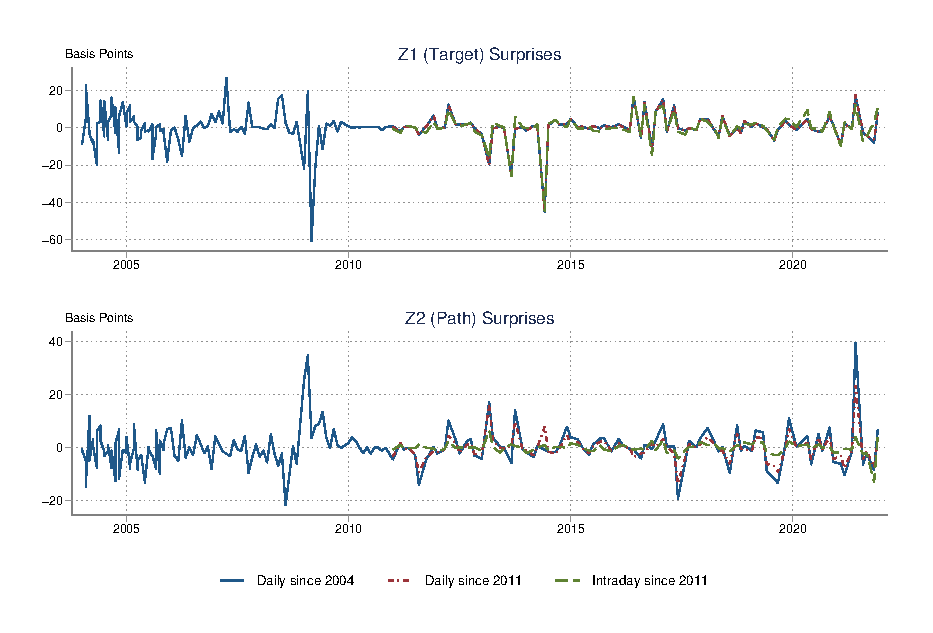
\includegraphics[width=1\textwidth,height=.4\textheight]{../Figures/factorslines.eps} \\
				\end{center}
				\vspace{-0.4cm}
				\fignotes{This figure compares the evolution of the \( \rtdone \) (target) and \( \rtdtwo \) (path) surprises obtained with daily data since 2004 (solid line) and 2011 (dash-dotted line), and with intraday data since 2011 (dashed line). The sample includes all regular monetary policy announcements up to \lastobs{}.}
			\end{minipage}
		\end{center}
	\end{figure}
\end{document}
% trim = {<left> <lower> <right> <upper>}
	% \ref{fig:factorslines}


\subsection{Interpreting the Factors} \label{sec:interpretation}
\iftoggle{toclinks}{\gototoc}{} % Turn it on/off in packages.tex, command in macros.tex
The factors \(\rtdone\) and \(\rtdtwo\) are henceforth referred to as the target and path factors or surprises. 
By definition, \(\rtdone\) moves one-to-one with surprises in the 3-month swap. \textcite{Solis:FX} shows that asset prices in Mexico respond to those surprises. 
Accordingly, \(\rtdone\) can be related to surprises in the \textit{current} policy rate, as it adequately captures the monetary stance in the short run. 
On the other hand, \(\rtdtwo\) is aligned with surprises in the 12-month swap that are unrelated to changes in the 3-month swap, so the second factor in principle might just capture a link to long-term yields.\footnote{ By construction, \(\rtdone\) is essentially the same as the policy rate surprises in \textcite{Solis:FX}, the correlation coefficient between the two measures is \(0.997\). Meanwhile, the correlation between \(\rtdtwo\) and the residual of a regression of the change in the 12-month swap on the change in the 3-month swap is \(0.85\).} %even though the 3-month swap might encompass more than one policy meeting ahead 
However, figure \ref{fig:factorspoints} and table \ref{tab:statements} support its association with surprises about the \textit{future} path of the policy rate.\footnote{\textcite{GSS:2005a} show that the first and second factors in the U.S. also relate to changes in the policy rate and about its future path communicated via statements, respectively.} 
In general, path surprises from emerging market central banks could be considered as communication surprises or as a subtle form of forward guidance.\footnote{Table \ref{tab:ranktests} does not support a third factor, which could be associated with asset purchases \parencite{Swanson:2021}. Several emerging market central banks indeed implemented asset purchases following the Covid pandemic akin to the ones in advanced economies after the global financial crisis \parencite{RebucciHartleyJimenez:2021}. Banxico made two such extraordinary announcements in March and April 2020, but they are excluded from the sample since it only comprises regular meetings.} 

Figure \ref{fig:factorspoints} compares the estimated target and path surprises for relevant dates over the sample period. 
While the analysis in sections \ref{sec:assets} and \ref{sec:flows} uses target and path surprises obtained using intraday data for efficiency in the estimation, the factors plotted in figure \ref{fig:factorspoints} are obtained using daily data (solid line in figure \ref{fig:factorslines}) in order to explore longer series (since 2004) in the interpretation of path surprises in section \ref{sec:pathsurprises}. 
In the figure, target surprises are in the horizontal axis, and path surprises are in the vertical axis; the units are basis points.\footnote{Target and path surprises are orthogonal to each other by construction, so no correlation is to be expected between the dots in the figure.}  
A positive value in any of the two surprises represents a tightening in Banxico's monetary stance, and a negative value represents an easing. 

Banxico has used all four possible combinations of target and path surprises. 
The first quadrant shows announcements in which there was a tightening in target as well as in path surprises, whereas both surprises eased in the third quadrant. 
In the second and fourth quadrants, there was a tightening in one surprise and an easing in the other. 

%\begin{center}
%	[Insert Figure \ref{fig:factorspoints} here.]
%\end{center}
\documentclass{article}
\usepackage{graphicx}
\usepackage[margin=1in]{geometry}
\usepackage[outdir=./]{epstopdf}  					% Avoids errors when input figures
\usepackage[labelsep=period,labelfont=bf]{caption}
%\usepackage{afterpage}
%\usepackage{subcaption}

\begin{document}
%	\afterpage{
	\begin{figure}[t]
		\caption{Monetary Policy Dimensions} \label{fig:factorspoints}
		\begin{center}								% center the minipage on the line
			\begin{minipage}{0.9\linewidth}
				\begin{center}							% center the figure inside the minipage
%					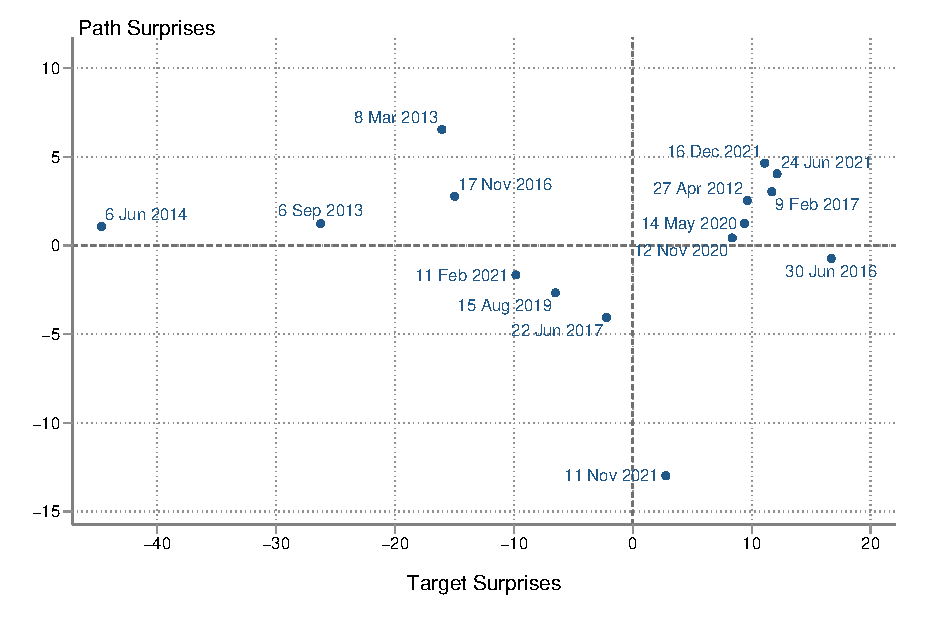
\includegraphics[width=1\textwidth,height=.4\textheight]{../Figures/factorspointstg.eps} \\
%					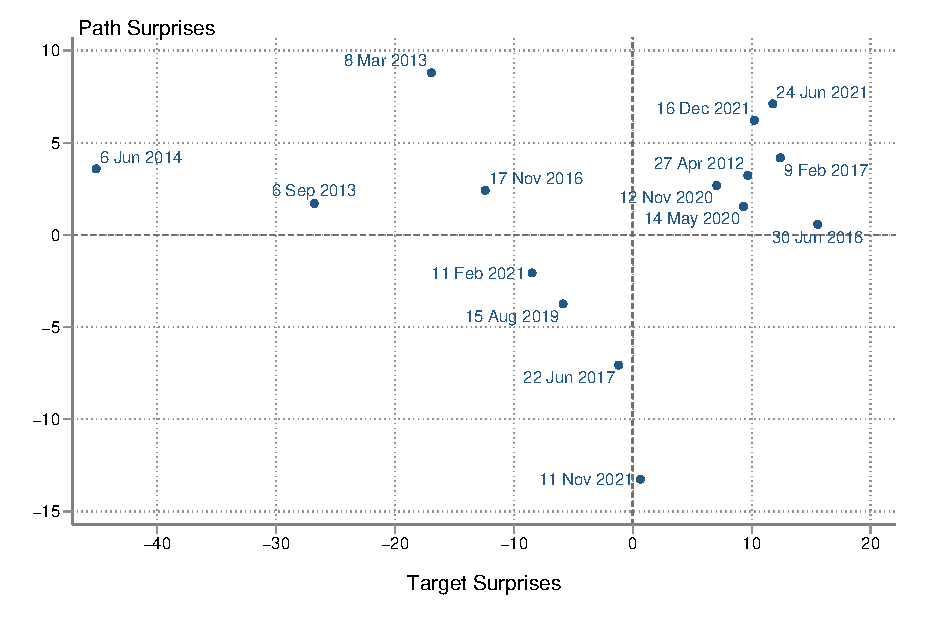
\includegraphics[width=1\textwidth,height=.4\textheight]{../Figures/factorspointswd.eps} \\
%					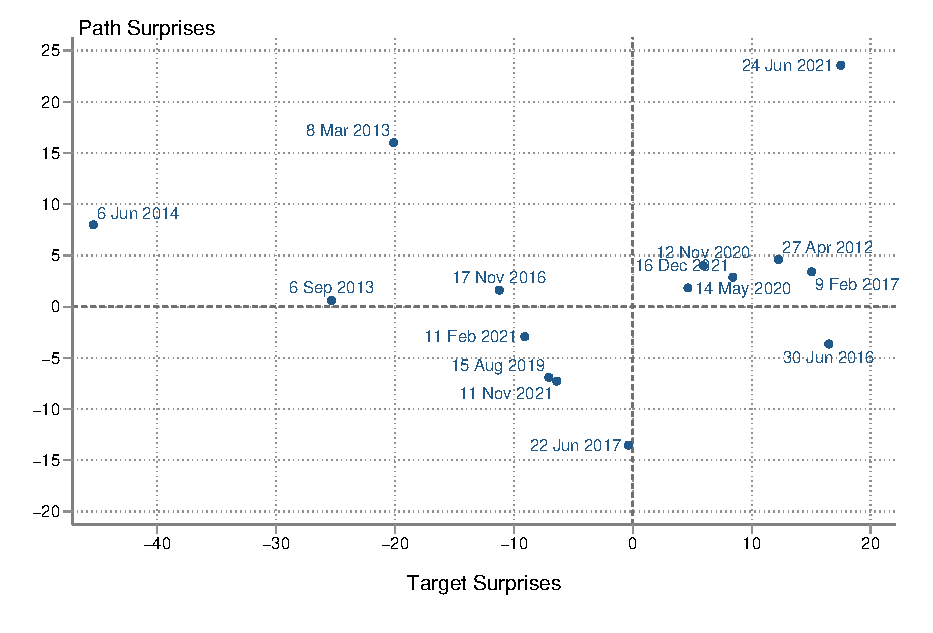
\includegraphics[width=1\textwidth,height=.4\textheight]{../Figures/factorspointsdy.eps} \\
					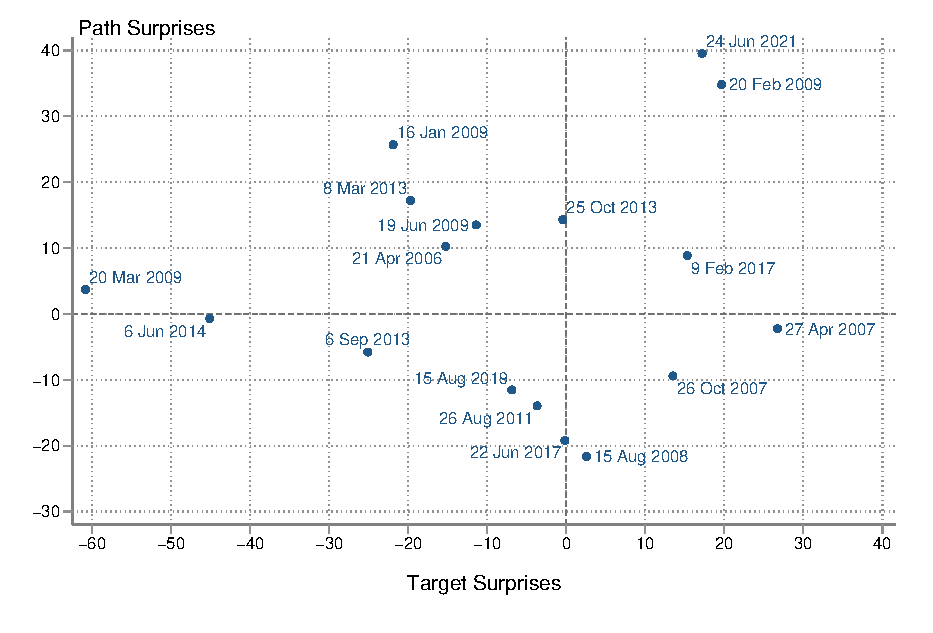
\includegraphics[width=1\textwidth,height=.4\textheight]{../Figures/factorspoints04.eps} \\
				\end{center}
				\vspace{-0.4cm}
				\fignotes{This figure plots the largest estimated target and path surprises (expressed in basis points) obtained from daily data, as explained in the main text. The sample includes all regular monetary policy announcements from January 2004 to \lastobs.} 
			\end{minipage}
		\end{center}
	\end{figure}
%	}
\end{document}
% trim = {<left> <lower> <right> <upper>}
	% \ref{fig:factorspoints}


\subsubsection{Statements and Path Surprises} \label{sec:pathsurprises}
Central bank statements convey information intended to influence expectations about future monetary policy decisions and to reduce policy uncertainty. 

Table \ref{tab:statements} shows that Banxico communicates information about the future path of the policy rate via statements. 
It summarizes the statements on announcement days in which, according to figure \ref{fig:factorspoints}, they communicated relevant information beyond the current policy rate. 
Notice that all the excerpts reported in the table contain clear references to the monetary stance in the future, and that several of them explicitly reference the future path of the policy rate.\footnote{Namely, the statements for June 2009, March and October 2013, February and June 2017.} 
The column labeled `Path' indicates whether figure \ref{fig:factorspoints} associates the respective statement with a tighter (\(+\)) or looser (\(-\)) monetary stance going forward.\footnote{Plotting the surprises obtained with daily (instead of intraday) data in figure \ref{fig:factorspoints} allows to assess the link between path surprises and statements over a longer period. Notice that half of the announcements in table \ref{tab:statements} are pre-2011, before the start of the sample period with intraday data.} 
Importantly, the excerpts and the signs are in line with each other, which is remarkable given that no textual analysis is involved in the identification of the surprises. 
%In particular, the statements accompanying the announcements on October 2007, August 2008 and 2011, and June 2017 suggested looser financial conditions ahead, while the statements for the rest of the announcements signaled a tighter monetary stance going forward. 

%\begin{center}
%	[Insert Table \ref{tab:statements} here.]
%\end{center}
\documentclass[a4paper,10pt]{article}
\usepackage[labelsep=period,labelfont=bf]{caption}
\usepackage{multirow}
\usepackage{booktabs}
\usepackage{longtable}
\usepackage{pdflscape}
\usepackage{afterpage}

\begin{document}
\afterpage{
\begin{normalsize}
\begin{landscape}
\begin{table}
\centering
\caption{Summary of Statements in Selected Dates}
\label{tab:statements}
\begin{tabular}{p{2.3cm} c p{17.5cm}}
\toprule
 Date & Path & Description \\
\midrule
21-Apr-2006 & \(+\) & Statement announces an easing of monetary conditions but notes that `for the foreseeable future there is no space available for further easing.' \\
26-Oct-2007 & \(-\) & Statement indicates that the risk that the sharp decline in the U.S. real estate market weakens the U.S. economy (affecting economic activity in Mexico) has increased. \\
15-Aug-2008 & \(-\) & Statement highlights that global inflationary pressures continue to rise but an improvement is foreseen in the medium term due to the prospects for lower global growth. Downside risks to the local economy have increased. \\
16-Jan-2009 & \(+\) & Statement notes `a higher than expected upward trend in inflation in the last quarter' and that `instability in financial markets continues to be a risk factor for the inflationary trend.' \\
20-Feb-2009 & \(+\) & Statement indicates that `the strong financial turmoil represents a risk to the expected inflation path, even considering the greater contraction in demand and the reduction in commodities prices.' \\
19-Jun-2009 & \(+\) & Statement indicates that `the Board considers that its easing cycle is close to an end.' \\
26-Aug-2011 & \(-\) & Statement notes that the current monetary policy stance is considered adequate but if it turns in an unnecessary tightening, the Board will reflect on the need to adjust it. \\
08-Mar-2013 & \(+\) & Statement makes clear that the 50 basis point reduction in the policy rate `does not represent the beginning of an easing cycle.' \\
25-Oct-2013 & \(+\) & Statement highlights that `no further cuts in the policy rate are appropriate in the foreseeable future.' \\
09-Feb-2017 & \(+\) & Statement highlights the effects of the tightenings in 2016 and `the ones required in 2017' to counteract inflationary pressures. \\
22-Jun-2017 & \(-\) & Statement drops reference to do `the necessary tightenings ahead' from the previous statement. \\
24-Jun-2021 & \(+\) & Statement highlights additional shocks to those expected in headline and core inflation, and notes that their expected paths in the following quarters are higher than previously estimated. \\
\bottomrule
\end{tabular}
\end{table}
\end{landscape}
\end{normalsize}
}
\end{document}
		% \ref{tab:statements}
%. browse date actual mxonbr expctsvymd expctsvyav target path 

%The announcements on April 2006, June 2009, March and October 2013, %January 2015 
%and February and June 2017 are noteworthy because of their explicit reference to the future path of the policy rate.

The tightening cycle that started in mid-2016 due to rising inflation risks exemplifies the link between path surprises and the information contained in statements. 
The 2016 U.S. presidential election generated uncertainty about the bilateral relation of the two countries. Between early-November 2016 and mid-January 2017, the peso depreciated by more than 14\%. 
In addition, the Mexican government raised the minimum wage and ended gasoline subsidies in early-2017. By mid-2017, inflation had risen for 10 consecutive months. %ln(21.89)-ln(19.1) = 13.63\% from Nov 1 to Jan 19.
In that context, Banxico raised its policy rate by 50 basis points on June and September 2016, more than the market expected according to surveys, followed by six more consecutive tightenings (three of 50 and three of 25 basis points). %\footnote{ The beginning of the tightening cycle might be dated as of November 2016 according to table \ref{tab:statements}.} 
In the statement for the last hike on June 22, 2017, Banxico dropped the reference to do `the necessary tightenings ahead' from the previous statement and indicated that it expected inflation to peak in the near future. The hike was mostly anticipated by the market (i.e., a null target surprise), but the wording of the statement suggested the end of the tightening cycle, essentially delivering a `pure' path easing surprise (see figure \ref{fig:factorspoints}).

Statements can also be associated with null path surprises. 
Contrary to survey expectations of no change in the policy rate, on June 6, 2014, Banxico cut the rate by 50 basis points, but in the statement indicated that `no further reductions in the policy rate are expected in the foreseeable future.' Therefore, the policy rate was cut unexpectedly, but the statement portrayed the decision as a one-off cut, essentially delivering a `pure' target surprise (see figure \ref{fig:factorspoints}). % Similar to September 6, 2013, Banxico announced a 25-basis-point cut in the policy rate but indicated that with `the lower policy rate, the monetary stance is in line with inflation converging to the target.'

In sum, target surprises capture unanticipated changes in the policy rate, while path surprises relate to news about its future path communicated via statements. 

%Since Banxico is an inflation targeter, the balance of risks for inflation plays a key role in managing the expectations about the future path of monetary policy. Factors affecting inflation therefore receive a lot of attention. One of those factors is the exchange rate. Banxico closely monitors the exchange rate since depreciations of the currency are usually associated with rising inflation.\footnote{ Notwithstanding, the pass-through of the exchange rate to inflation has been generally low in Mexico.} Local supply shocks also represent upward risks to inflation.\footnote{ Examples include increases in the minimum wage in 2017 and 2019, and a reform that ended gasoline subsidies.} Along with others, these risks play an important role in central bank communications.
% Low pass-through highlighted in 20jan2012 statement. The rise in the minimum wage happened in January 2017.

%Notice two things. First, tightening path surprises have been more common than easing path surprises over the sample period. Second, notice that the magnitude of the path surprises is lower than that of target surprises. The largest path surprises in Mexico are also lower compared to the largest path surprises for the U.S. reported by \textcite{GSS:2005a}, see their table 4. 
%Two potential reasons might explain this.
%First, international developments play a relevant role in the monetary policy considerations of small open economies, and Mexico is no exception. In this sense, it is harder to commit to a future path of the policy rate for extended periods of time when there is high uncertainty abroad.
%Second, and most importantly, the possibility of reaching the zero lower bound has not been an issue in Mexico, and so the need of Banxico to rely on path surprises has been low.

}{}	% Closes \iftoggle{fulldraft}


\section{The Effects of Monetary Policy on Asset Prices} \label{sec:assets}
\iftoggle{toclinks}{\gototoc}{} % Turn it on/off in packages.tex, command in macros.tex
The previous section shows that target and path surprises capture the responses of asset prices to monetary policy decisions.
This section quantifies the response of the exchange rate and the yield curve to those surprises. 
The next section deals with portfolio flows.

\iftoggle{fulldraft}{					% Turn it on/off in packages.tex
	
\subsection{Contemporaneous Effects}
The following event-study regression measures the on-impact effects of the two types of monetary policy surprises on the exchange rate and the yield curve:
\begin{equation} \label{eq:nTwoFacP}
	\eqTwoFacP ,
\end{equation}	%(\ref{eq:nTwoFacP})
\noindent in which \(\depvar\) is the intraday change in asset prices around monetary policy announcements, as described in section \ref{sec:mpsidentification}. 
\(\rtdonereg\) and \(\rtdtworeg\) are the two types of surprises %described in section \ref{sec:interpretation} 
obtained using intraday data.\footnote{As already mentioned, even though the surprises can also be obtained from daily data over a larger sample size, the analysis uses the surprises obtained with intraday data because there are gains in precision during the estimation and in terms of explanatory power.} 
All the variables are expressed in basis points. 
Finally, the error term \(\errorreg\) captures variations in the dependent variables unrelated to the two surprises. 

Table \ref{tab:fctrsfxyc} reports the results of the estimation. The first column for each dependent variable shows the coefficient estimates when the regression only includes target surprises as the independent variable, while the second column adds path surprises as a regressor. 
Focusing on the first column, a target tightening surprise appreciates the currency and flattens the yield curve. 
As expected, the estimated coefficients for the target surprises are consistent with the ones reported by \textcite[][Table 2]{Solis:FX} for the policy rate surprises.\footnote{\textcite{Solis:FX} defines the policy rate surprises as the intraday changes in the 3-month swap. Remember that the target factor is rescaled so that it moves one-to-one with the changes in the 3-month swap.} 

%\begin{center}
%	[Insert Table \ref{tab:fctrsfxyc} here.]
%\end{center}
\documentclass[a4paper,12pt]{article}
\usepackage[labelsep=period,labelfont=bf]{caption}
\usepackage{multirow}
\usepackage{booktabs}
\usepackage{threeparttable}
\usepackage{pdflscape}
\usepackage{tabularx}
\usepackage{afterpage}
\usepackage[margin=1in]{geometry}
%% Personalized Macros
% Table of Contents, Tables, Subcaptions, Track Changes, Footnotes

%---------------------------------------------------------------
% Table of Contents
%---------------------------------------------------------------

% Link to ToC from section
\newcommand{\gototoc}{\vspace{-2cm} \null\hfill [\hyperlink{toc}{Go2ToC}] \newline}

% Link back to section from ToC
\newcommand{\maketoc}{
	\hypertarget{toc}{}
	\newpage
	\tableofcontents
	\vspace{2.5\bigskipamount} }

% Box with bullets for tasks to do in a section
\newenvironment{boxeditems}
	{\begin{tabular}{|p{\linewidth}|}
	\hline
	\begin{itemize}
	}
	{
	\end{itemize}
	\\ \hline
	\end{tabular} \\
	}

%---------------------------------------------------------------
% Tables
%---------------------------------------------------------------

% Estout Commands following Jörg Weber
\newcommand{\sym}[1]{\rlap{#1}}

\let\estinput=\input	% define new input command to flatten the document

\newcommand{\estauto}[2]{
	\newcolumntype{C}{>{\centering\arraybackslash}X}
	\vspace{.75ex}{
%		\begin{tabularx}{1.4\textwidth}{l*{#2}C}
		\begin{tabularx}{0.95\linewidth}{l*{#2}C}
			\toprule
			\estinput{#1}
			\\ \bottomrule
			\addlinespace[.75ex]
		\end{tabularx}
	}
}

% Allow line breaks with \\ in specialcells
\newcommand{\specialcell}[2][c]{\begin{tabular}[#1]{@{}c@{}}#2\end{tabular}}

%---------------------------------------------------------------
% Subcaptions
%---------------------------------------------------------------

% Notes after figures following Jörg Weber
\newcommand{\figtext}[1]{
	\vspace{-1ex}
	\captionsetup{justification=justified,font=footnotesize}
	\caption*{#1}
%	\captionsetup{justification=raggedright,singlelinecheck=false,font=footnotesize}
%	\caption*{\hspace{6pt}\hangindent=1.5em #1}
}

\newcommand{\fignote}[1]{\figtext{\emph{Note:~}~#1}}
\newcommand{\fignotes}[1]{\figtext{\emph{Notes:~}~#1}}

% Notes after tables
\newcommand{\tabnote}[1]{
	\begin{tablenotes}[para,flushleft]
		\footnotesize \emph{Notes:~}~#1
	\end{tablenotes}
}

%---------------------------------------------------------------
% Track Changes
%---------------------------------------------------------------

% Highlight changes in revised version with color
\newcommand{\textchange}[1]{\iftoggle{revised}{\textcolor{blue}{#1}}{#1}}

%---------------------------------------------------------------
% Footnotes
%---------------------------------------------------------------

%% Change the look of foonote indicators
%\makeatletter
%\let \@makefntextorig \@makefntext
%\newcommand{\@makefntextcustom}[1]{%
%	\thefootnote.\enskip #1%
%}
%\renewcommand{\@makefntext}[1]{\@makefntextcustom{#1}}
%\makeatother
%
%% Change the look of endnote indicators
%\renewcommand{\makeenmark}{\hbox{$^{\theenmark}$}}
%\makeatletter
%\def\enoteformat{%
%	\rightskip\z@ \leftskip\z@ \parindent=1.8em
%	\leavevmode{\setbox\z@=\lastbox}\llap{\theenmark.\enskip}%
%}
%\makeatother			   % Personalized commands
%% Personalized Macros
% Variable Definitions, Equations

%---------------------------------------------------------------
% Variable Definitions
%---------------------------------------------------------------
\providecommand{\tiie}{TIIE28D}
\providecommand{\lastobs}{December 2021}
\providecommand{\lastobsfx}{November 2021}
\providecommand{\lastobsflwbdm}{December 2021}
\providecommand{\lastobsflwtic}{August 2021}
\providecommand{\idxt}{t}
\providecommand{\idxh}{h}
\providecommand{\idxi}{i}
\providecommand{\idxsfwd}{\idxt+\idxh}
\providecommand{\idxslag}{\idxt-1}
\providecommand{\yld}{y}
\providecommand{\ctrls}{z}
\providecommand{\hld}{H}
\providecommand{\depvar}{\Delta \yld_{\idxt}}
\providecommand{\mps}{\Delta x_{\idxt}}
\providecommand{\depvarclean}{\depvar^{*}}
\providecommand{\mpsclean}{\mps^{*}}
\providecommand{\paramB}{\beta}
\providecommand{\intrcpt}{\paramB_{0}}
\providecommand{\slopetrgt}{\paramB_{1}}
\providecommand{\slopepath}{\paramB_{2}}
\providecommand{\assets}{X}
\providecommand{\factors}{F}
\providecommand{\loadings}{\Lambda}
\providecommand{\rotated}{Z}
\providecommand{\rmatrix}{U}
\providecommand{\rtdone}{\rotated_{1}}
\providecommand{\rtdtwo}{\rotated_{2}}
\providecommand{\rtdonereg}{Target_{\idxt}}
\providecommand{\rtdtworeg}{Path_{\idxt}}
\providecommand{\lagidx}{j}
\providecommand{\lagorder}{p}
\providecommand{\lagparam}{\gamma}   %\alpha
\providecommand{\lagoper}{L}
\providecommand{\depvarflw}{\Delta \hld_{\idxt}}
\providecommand{\flows}{w_{\idxt}}
\providecommand{\flowslag}{w_{\idxt - \lagidx}}
\providecommand{\lagsum}{\sum_{\lagidx = 1}^{\lagorder} \lagparam_{\lagidx} \flowslag}
\providecommand{\lagsumh}{\sum_{\lagidx = 1}^{\lagorder} \lagparam^{\lagidx}_\idxh \flowslag}
\providecommand{\dimobs}{T}
\providecommand{\dimassets}{n}
\providecommand{\dimfactors}{k}
\providecommand{\dimnull}{\dimfactors_{0}}
\providecommand{\dimsassets}{\dimobs \times \dimassets}
\providecommand{\dimsfactors}{\dimobs \times \dimfactors}
\providecommand{\dimsloadings}{\dimfactors \times \dimassets}
\providecommand{\errorreg}{\varepsilon_{\idxt}}
\providecommand{\errorfac}{\zeta}
\providecommand{\errorflows}{\nu_{\idxt}}
\providecommand{\Rsqrt}{R^{2}}

\providecommand{\dpv}{y}
\providecommand{\idv}{x}
\providecommand{\omv}{\omega}
\providecommand{\dpvstar}{\dpv^{*}}
\providecommand{\idvstar}{\idv^{*}}
\providecommand{\jobs}{Jobs}
\providecommand{\errortrue}{\varepsilon}
\providecommand{\errormix}{\tau}
\providecommand{\melhs}{\nu}
\providecommand{\merhs}{u}
\providecommand{\mean}{\mu}
\providecommand{\covar}{\sigma}
\providecommand{\corr}{\rho}
\providecommand{\var}{\covar^{2}}
\providecommand{\meanE}{\mean_{\errortrue}}
\providecommand{\meanU}{\mean_{\merhs}}
\providecommand{\meanV}{\mean_{\melhs}}
\providecommand{\varE}{\var_{\errortrue}}
\providecommand{\varU}{\var_{\merhs}}
\providecommand{\varV}{\var_{\melhs}}
\providecommand{\varX}{\var_{\idv}}
\providecommand{\varXstar}{\var_{\idvstar}}
\providecommand{\covarEX}{\covar_{\errortrue \idvstar}}
\providecommand{\covarUE}{\covar_{\merhs \errortrue}}
\providecommand{\covarVE}{\covar_{\melhs \errortrue}}
\providecommand{\covarUX}{\covar_{\merhs \idvstar}}
\providecommand{\covarUY}{\covar_{\merhs \dpvstar}}
\providecommand{\covarVX}{\covar_{\melhs \idvstar}}
\providecommand{\covarVY}{\covar_{\melhs \dpvstar}}
\providecommand{\covarUV}{\covar_{\merhs \melhs}}
\providecommand{\covarWXe}{\covar_{\omv \idv}}
\providecommand{\covarVXe}{\covar_{\melhs \idv}}
\providecommand{\corrUV}{\corr_{\merhs \melhs}}
\providecommand{\corrUX}{\corr_{\merhs \idvstar}}
\providecommand{\corrUY}{\corr_{\merhs \dpvstar}}
\providecommand{\corrVX}{\corr_{\melhs \idvstar}}
\providecommand{\corrVY}{\corr_{\melhs \dpvstar}}
\providecommand{\paramG}{\gamma}
\providecommand{\estimB}{\hat{\paramB}}
\providecommand{\paramSE}{\varE}
\providecommand{\estimSE}{\hat{\paramSE}}
\providecommand{\paramAVB}{s}
\providecommand{\estimAVB}{\hat{\paramAVB}}
\providecommand{\attnfactor}{\lambda}
\providecommand{\plim}{\mathrm{plim}}

\providecommand{\reg}{\delta}
\providecommand{\regVonX}{\reg_{\melhs \idv}}
\providecommand{\regWonX}{\reg_{\omv \idv}}
\providecommand{\regWonXstar}{\reg_{\omv \idvstar}}

%---------------------------------------------------------------
% Equations
%---------------------------------------------------------------
\newcommand{\eqOneFac}{\depvar = \intrcpt + \slopetrgt \mps + \errorreg}
\newcommand{\eqOneFacOV}{\depvar = \intrcpt + \slopetrgt PRS_{\idxt} + \paramB_{2} \Delta VIX_{\idxt} + \paramB_{3} \Delta USY_{\idxt} + \paramB_{4} WTI_{\idxt} + \paramB_{5} \jobs_{\idxt} + \errorreg}
\newcommand{\eqTwoFacP}{\depvar = \intrcpt + \slopetrgt \rtdonereg + \slopepath \rtdtworeg + \errorreg}
\newcommand{\eqTwoFacF}{\depvarflw = \intrcpt + \slopetrgt \rtdonereg + \slopepath \rtdtworeg + \errorreg}
\newcommand{\eqPCA}{\assets = \factors \loadings + \errorfac}
\newcommand{\eqRotation}{\rotated = \factors \, \rmatrix}
\newcommand{\eqFlows}{\flows = \intrcpt + \slopetrgt \rtdonereg + \slopepath \rtdtworeg + \lagsum + \eta^{'} \ctrls_{\idxslag} + \errorflows}
%\newcommand{\eqLagPoly}{\lagsum = 1 - \lagparam_{1} \lagoper - \lagparam_{2} \lagoper^{2} - \ldots - \lagparam_{\lagorder} \lagoper^{\lagorder}}
\newcommand{\eqAsym}{\yld_{\idxt} = \intrcpt + \paramB_{1} \rtdonereg \mathds{1} \left(\rtdonereg > 0 \right) + \paramB_{2} \rtdonereg \mathds{1} \left(\rtdonereg < 0 \right) \\ + \paramB_{3} \rtdtworeg \mathds{1} \left(\rtdtworeg > 0 \right) + \paramB_{4} \rtdtworeg \mathds{1} \left(\rtdtworeg < 0 \right) + \errorreg}

\newcommand{\eqDGP}{\dpvstar &= \paramB \idvstar + \errortrue}
\newcommand{\eqDGPme}{\dpv = \paramB \idv + \errormix = \paramB \idv + \eqErrormix}
\newcommand{\eqDGPov}{\dpvstar = \paramB \idvstar + \paramG \omv +  \errortrue}
\newcommand{\eqMEdpv}{\dpv &= \dpvstar + \melhs}
\newcommand{\eqMEidv}{\idv &= \idvstar + \merhs}
\newcommand{\eqAtten}{\attnfactor = \frac{\varXstar}{\varXstar + \varU}}
\newcommand{\eqAttenInLine}{\attnfactor = \varXstar / \left(\varXstar + \varU\right) }
\newcommand{\eqErrormix}{\errortrue - \paramB \merhs + \melhs}

\newcommand{\eqPlimBstd}{\plim \left( \estimB \right) = \frac{cov(\idv, \dpvstar)}{var(\idv)} = \frac{cov(\idvstar + \merhs, \paramB \idvstar + \errortrue)}{var(\idvstar + \merhs)} = \paramB \frac{\varXstar}{\varXstar + \varU} = \paramB \attnfactor}
\newcommand{\eqPlimBstdshort}{\plim (\estimB) = \paramB \attnfactor}

%\newcommand{\eqPlimSstd}{\plim \left( \estimAVB \right) = \plim \left( \frac{\estimSE}{\hat{\varX}} \right) = \frac{\varE + (1-\attnfactor)^{2} \paramB^{2} \varXstar + \attnfactor^{2} \paramB^{2} \varU}{\varXstar + \varU} = \attnfactor \paramAVB + \attnfactor(1 - \attnfactor) \paramB^{2}}
\newcommand{\eqPlimSstd}{\plim \left( \estimAVB \right) = \attnfactor \paramAVB + \attnfactor(1 - \attnfactor) \paramB^{2}}

\newcommand{\eqPlimBnew}{\plim \left( \estimB \right) 
	= \frac{cov(\idv, \dpv)}{var(\idv)} 
	= \frac{cov(\idvstar + \merhs, \paramB \idvstar + \paramG \omv + \errortrue)}{var(\idvstar + \merhs)} 
	= \frac{\paramB \varXstar + \paramG \covarWXe}{\varXstar + \varU}  }

\newcommand{\eqPlimBbias}{\plim \left( \estimB \right)
	= \paramB \frac{\varXstar}{\varX} + \paramG \frac{\covarWXe}{\varX}
	= \paramB \attnfactor + \paramG \regWonX}

\providecommand{\errordepvar}{e_{y}}
\providecommand{\errormps}{e_{x}}
\newcommand{\eqMEdepvar}{\depvar &= \depvarclean + \errordepvar}
\newcommand{\eqMEmps}{\mps &= \mpsclean + \errormps}

\newcommand{\eqLPrhs}{\alpha_{\idxh} + \beta^{1}_{\idxh} \; \rtdonereg +  \beta^{2}_{\idxh} \; \rtdtworeg + \eta^{'}_{\idxh} \ctrls_{\idxslag}  + u_{\idxsfwd}}

\newcommand{\eqLPprices}{\yld_{\idxsfwd} - \yld_{\idxslag} = \eqLPrhs} 

\newcommand{\eqLPflows}{\hld_{\idxsfwd} - \hld_{\idxslag} = \eqLPrhs} 
% \gamma_{\idxh} \Delta \yld_{\idxslag} 
%\alpha_{\idxh} + \beta^{1}_{\idxh} \; \rtdonereg +  \beta^{2}_{\idxh} \; \rtdtworeg + \lagsumh + \eta_{\idxh} \ctrls_{\idxslag}  + u_{\idxsfwd}

\newcommand{\eqLP}{\yld_{\idxsfwd} - \yld_{\idxslag} = \alpha_{\idxh} + \gamma_{\idxh} \mps + u_{\idxsfwd}} 			    % Personalized commands
%\pagestyle{empty}

\begin{document}
	\afterpage{
	\begin{normalsize}
		\begin{landscape}
			\begin{table}
				\begin{center}
					\caption{Response of Asset Prices to Target and Path Surprises} \label{tab:fctrsfxyc} %: Intraday Data
					\begin{threeparttable}
						\estauto{../Tables/f_fctrsfxyc.tex}{10}
						\tabnote{The first column for each dependent variable shows the coefficient estimates in regressions of intraday yield changes or exchange rate (FX) returns on target surprises; the second column adds path surprises as a regressor. Target and path surprises are obtained from intraday data, as explained in the main text. Intraday changes are calculated starting 10 minutes before to 20 minutes after a monetary policy announcement. The sample includes all regular monetary policy announcements starting on January 2011 for the exchange rate, on January 2013 for 2- 10- and 30-year yields, and on December 2014 for 5-year yields; the sample ends on \lastobs{} in all cases. Figures are expressed in basis points. Heteroskedasticity-robust standard errors are shown in parentheses. *, **, *** asterisks respectively indicate significance at the 10\%, 5\% and 1\% level.}
					\end{threeparttable}
				\end{center}
			\end{table}
		\end{landscape}
	\end{normalsize}
	}
\end{document}		% Intraday changes on intraday surprises

%\documentclass[a4paper,12pt]{article}
\usepackage[labelsep=period,labelfont=bf]{caption}
\usepackage{multirow}
\usepackage{booktabs}
\usepackage{threeparttable}
\usepackage{pdflscape}
\usepackage{tabularx}
\usepackage[margin=1in]{geometry}
%% Personalized Macros
% Table of Contents, Tables, Subcaptions, Track Changes, Footnotes

%---------------------------------------------------------------
% Table of Contents
%---------------------------------------------------------------

% Link to ToC from section
\newcommand{\gototoc}{\vspace{-2cm} \null\hfill [\hyperlink{toc}{Go2ToC}] \newline}

% Link back to section from ToC
\newcommand{\maketoc}{
	\hypertarget{toc}{}
	\newpage
	\tableofcontents
	\vspace{2.5\bigskipamount} }

% Box with bullets for tasks to do in a section
\newenvironment{boxeditems}
	{\begin{tabular}{|p{\linewidth}|}
	\hline
	\begin{itemize}
	}
	{
	\end{itemize}
	\\ \hline
	\end{tabular} \\
	}

%---------------------------------------------------------------
% Tables
%---------------------------------------------------------------

% Estout Commands following Jörg Weber
\newcommand{\sym}[1]{\rlap{#1}}

\let\estinput=\input	% define new input command to flatten the document

\newcommand{\estauto}[2]{
	\newcolumntype{C}{>{\centering\arraybackslash}X}
	\vspace{.75ex}{
%		\begin{tabularx}{1.4\textwidth}{l*{#2}C}
		\begin{tabularx}{0.95\linewidth}{l*{#2}C}
			\toprule
			\estinput{#1}
			\\ \bottomrule
			\addlinespace[.75ex]
		\end{tabularx}
	}
}

% Allow line breaks with \\ in specialcells
\newcommand{\specialcell}[2][c]{\begin{tabular}[#1]{@{}c@{}}#2\end{tabular}}

%---------------------------------------------------------------
% Subcaptions
%---------------------------------------------------------------

% Notes after figures following Jörg Weber
\newcommand{\figtext}[1]{
	\vspace{-1ex}
	\captionsetup{justification=justified,font=footnotesize}
	\caption*{#1}
%	\captionsetup{justification=raggedright,singlelinecheck=false,font=footnotesize}
%	\caption*{\hspace{6pt}\hangindent=1.5em #1}
}

\newcommand{\fignote}[1]{\figtext{\emph{Note:~}~#1}}
\newcommand{\fignotes}[1]{\figtext{\emph{Notes:~}~#1}}

% Notes after tables
\newcommand{\tabnote}[1]{
	\begin{tablenotes}[para,flushleft]
		\footnotesize \emph{Notes:~}~#1
	\end{tablenotes}
}

%---------------------------------------------------------------
% Track Changes
%---------------------------------------------------------------

% Highlight changes in revised version with color
\newcommand{\textchange}[1]{\iftoggle{revised}{\textcolor{blue}{#1}}{#1}}

%---------------------------------------------------------------
% Footnotes
%---------------------------------------------------------------

%% Change the look of foonote indicators
%\makeatletter
%\let \@makefntextorig \@makefntext
%\newcommand{\@makefntextcustom}[1]{%
%	\thefootnote.\enskip #1%
%}
%\renewcommand{\@makefntext}[1]{\@makefntextcustom{#1}}
%\makeatother
%
%% Change the look of endnote indicators
%\renewcommand{\makeenmark}{\hbox{$^{\theenmark}$}}
%\makeatletter
%\def\enoteformat{%
%	\rightskip\z@ \leftskip\z@ \parindent=1.8em
%	\leavevmode{\setbox\z@=\lastbox}\llap{\theenmark.\enskip}%
%}
%\makeatother			   % Personalized commands
%% Personalized Macros
% Variable Definitions, Equations

%---------------------------------------------------------------
% Variable Definitions
%---------------------------------------------------------------
\providecommand{\tiie}{TIIE28D}
\providecommand{\lastobs}{December 2021}
\providecommand{\lastobsfx}{November 2021}
\providecommand{\lastobsflwbdm}{December 2021}
\providecommand{\lastobsflwtic}{August 2021}
\providecommand{\idxt}{t}
\providecommand{\idxh}{h}
\providecommand{\idxi}{i}
\providecommand{\idxsfwd}{\idxt+\idxh}
\providecommand{\idxslag}{\idxt-1}
\providecommand{\yld}{y}
\providecommand{\ctrls}{z}
\providecommand{\hld}{H}
\providecommand{\depvar}{\Delta \yld_{\idxt}}
\providecommand{\mps}{\Delta x_{\idxt}}
\providecommand{\depvarclean}{\depvar^{*}}
\providecommand{\mpsclean}{\mps^{*}}
\providecommand{\paramB}{\beta}
\providecommand{\intrcpt}{\paramB_{0}}
\providecommand{\slopetrgt}{\paramB_{1}}
\providecommand{\slopepath}{\paramB_{2}}
\providecommand{\assets}{X}
\providecommand{\factors}{F}
\providecommand{\loadings}{\Lambda}
\providecommand{\rotated}{Z}
\providecommand{\rmatrix}{U}
\providecommand{\rtdone}{\rotated_{1}}
\providecommand{\rtdtwo}{\rotated_{2}}
\providecommand{\rtdonereg}{Target_{\idxt}}
\providecommand{\rtdtworeg}{Path_{\idxt}}
\providecommand{\lagidx}{j}
\providecommand{\lagorder}{p}
\providecommand{\lagparam}{\gamma}   %\alpha
\providecommand{\lagoper}{L}
\providecommand{\depvarflw}{\Delta \hld_{\idxt}}
\providecommand{\flows}{w_{\idxt}}
\providecommand{\flowslag}{w_{\idxt - \lagidx}}
\providecommand{\lagsum}{\sum_{\lagidx = 1}^{\lagorder} \lagparam_{\lagidx} \flowslag}
\providecommand{\lagsumh}{\sum_{\lagidx = 1}^{\lagorder} \lagparam^{\lagidx}_\idxh \flowslag}
\providecommand{\dimobs}{T}
\providecommand{\dimassets}{n}
\providecommand{\dimfactors}{k}
\providecommand{\dimnull}{\dimfactors_{0}}
\providecommand{\dimsassets}{\dimobs \times \dimassets}
\providecommand{\dimsfactors}{\dimobs \times \dimfactors}
\providecommand{\dimsloadings}{\dimfactors \times \dimassets}
\providecommand{\errorreg}{\varepsilon_{\idxt}}
\providecommand{\errorfac}{\zeta}
\providecommand{\errorflows}{\nu_{\idxt}}
\providecommand{\Rsqrt}{R^{2}}

\providecommand{\dpv}{y}
\providecommand{\idv}{x}
\providecommand{\omv}{\omega}
\providecommand{\dpvstar}{\dpv^{*}}
\providecommand{\idvstar}{\idv^{*}}
\providecommand{\jobs}{Jobs}
\providecommand{\errortrue}{\varepsilon}
\providecommand{\errormix}{\tau}
\providecommand{\melhs}{\nu}
\providecommand{\merhs}{u}
\providecommand{\mean}{\mu}
\providecommand{\covar}{\sigma}
\providecommand{\corr}{\rho}
\providecommand{\var}{\covar^{2}}
\providecommand{\meanE}{\mean_{\errortrue}}
\providecommand{\meanU}{\mean_{\merhs}}
\providecommand{\meanV}{\mean_{\melhs}}
\providecommand{\varE}{\var_{\errortrue}}
\providecommand{\varU}{\var_{\merhs}}
\providecommand{\varV}{\var_{\melhs}}
\providecommand{\varX}{\var_{\idv}}
\providecommand{\varXstar}{\var_{\idvstar}}
\providecommand{\covarEX}{\covar_{\errortrue \idvstar}}
\providecommand{\covarUE}{\covar_{\merhs \errortrue}}
\providecommand{\covarVE}{\covar_{\melhs \errortrue}}
\providecommand{\covarUX}{\covar_{\merhs \idvstar}}
\providecommand{\covarUY}{\covar_{\merhs \dpvstar}}
\providecommand{\covarVX}{\covar_{\melhs \idvstar}}
\providecommand{\covarVY}{\covar_{\melhs \dpvstar}}
\providecommand{\covarUV}{\covar_{\merhs \melhs}}
\providecommand{\covarWXe}{\covar_{\omv \idv}}
\providecommand{\covarVXe}{\covar_{\melhs \idv}}
\providecommand{\corrUV}{\corr_{\merhs \melhs}}
\providecommand{\corrUX}{\corr_{\merhs \idvstar}}
\providecommand{\corrUY}{\corr_{\merhs \dpvstar}}
\providecommand{\corrVX}{\corr_{\melhs \idvstar}}
\providecommand{\corrVY}{\corr_{\melhs \dpvstar}}
\providecommand{\paramG}{\gamma}
\providecommand{\estimB}{\hat{\paramB}}
\providecommand{\paramSE}{\varE}
\providecommand{\estimSE}{\hat{\paramSE}}
\providecommand{\paramAVB}{s}
\providecommand{\estimAVB}{\hat{\paramAVB}}
\providecommand{\attnfactor}{\lambda}
\providecommand{\plim}{\mathrm{plim}}

\providecommand{\reg}{\delta}
\providecommand{\regVonX}{\reg_{\melhs \idv}}
\providecommand{\regWonX}{\reg_{\omv \idv}}
\providecommand{\regWonXstar}{\reg_{\omv \idvstar}}

%---------------------------------------------------------------
% Equations
%---------------------------------------------------------------
\newcommand{\eqOneFac}{\depvar = \intrcpt + \slopetrgt \mps + \errorreg}
\newcommand{\eqOneFacOV}{\depvar = \intrcpt + \slopetrgt PRS_{\idxt} + \paramB_{2} \Delta VIX_{\idxt} + \paramB_{3} \Delta USY_{\idxt} + \paramB_{4} WTI_{\idxt} + \paramB_{5} \jobs_{\idxt} + \errorreg}
\newcommand{\eqTwoFacP}{\depvar = \intrcpt + \slopetrgt \rtdonereg + \slopepath \rtdtworeg + \errorreg}
\newcommand{\eqTwoFacF}{\depvarflw = \intrcpt + \slopetrgt \rtdonereg + \slopepath \rtdtworeg + \errorreg}
\newcommand{\eqPCA}{\assets = \factors \loadings + \errorfac}
\newcommand{\eqRotation}{\rotated = \factors \, \rmatrix}
\newcommand{\eqFlows}{\flows = \intrcpt + \slopetrgt \rtdonereg + \slopepath \rtdtworeg + \lagsum + \eta^{'} \ctrls_{\idxslag} + \errorflows}
%\newcommand{\eqLagPoly}{\lagsum = 1 - \lagparam_{1} \lagoper - \lagparam_{2} \lagoper^{2} - \ldots - \lagparam_{\lagorder} \lagoper^{\lagorder}}
\newcommand{\eqAsym}{\yld_{\idxt} = \intrcpt + \paramB_{1} \rtdonereg \mathds{1} \left(\rtdonereg > 0 \right) + \paramB_{2} \rtdonereg \mathds{1} \left(\rtdonereg < 0 \right) \\ + \paramB_{3} \rtdtworeg \mathds{1} \left(\rtdtworeg > 0 \right) + \paramB_{4} \rtdtworeg \mathds{1} \left(\rtdtworeg < 0 \right) + \errorreg}

\newcommand{\eqDGP}{\dpvstar &= \paramB \idvstar + \errortrue}
\newcommand{\eqDGPme}{\dpv = \paramB \idv + \errormix = \paramB \idv + \eqErrormix}
\newcommand{\eqDGPov}{\dpvstar = \paramB \idvstar + \paramG \omv +  \errortrue}
\newcommand{\eqMEdpv}{\dpv &= \dpvstar + \melhs}
\newcommand{\eqMEidv}{\idv &= \idvstar + \merhs}
\newcommand{\eqAtten}{\attnfactor = \frac{\varXstar}{\varXstar + \varU}}
\newcommand{\eqAttenInLine}{\attnfactor = \varXstar / \left(\varXstar + \varU\right) }
\newcommand{\eqErrormix}{\errortrue - \paramB \merhs + \melhs}

\newcommand{\eqPlimBstd}{\plim \left( \estimB \right) = \frac{cov(\idv, \dpvstar)}{var(\idv)} = \frac{cov(\idvstar + \merhs, \paramB \idvstar + \errortrue)}{var(\idvstar + \merhs)} = \paramB \frac{\varXstar}{\varXstar + \varU} = \paramB \attnfactor}
\newcommand{\eqPlimBstdshort}{\plim (\estimB) = \paramB \attnfactor}

%\newcommand{\eqPlimSstd}{\plim \left( \estimAVB \right) = \plim \left( \frac{\estimSE}{\hat{\varX}} \right) = \frac{\varE + (1-\attnfactor)^{2} \paramB^{2} \varXstar + \attnfactor^{2} \paramB^{2} \varU}{\varXstar + \varU} = \attnfactor \paramAVB + \attnfactor(1 - \attnfactor) \paramB^{2}}
\newcommand{\eqPlimSstd}{\plim \left( \estimAVB \right) = \attnfactor \paramAVB + \attnfactor(1 - \attnfactor) \paramB^{2}}

\newcommand{\eqPlimBnew}{\plim \left( \estimB \right) 
	= \frac{cov(\idv, \dpv)}{var(\idv)} 
	= \frac{cov(\idvstar + \merhs, \paramB \idvstar + \paramG \omv + \errortrue)}{var(\idvstar + \merhs)} 
	= \frac{\paramB \varXstar + \paramG \covarWXe}{\varXstar + \varU}  }

\newcommand{\eqPlimBbias}{\plim \left( \estimB \right)
	= \paramB \frac{\varXstar}{\varX} + \paramG \frac{\covarWXe}{\varX}
	= \paramB \attnfactor + \paramG \regWonX}

\providecommand{\errordepvar}{e_{y}}
\providecommand{\errormps}{e_{x}}
\newcommand{\eqMEdepvar}{\depvar &= \depvarclean + \errordepvar}
\newcommand{\eqMEmps}{\mps &= \mpsclean + \errormps}

\newcommand{\eqLPrhs}{\alpha_{\idxh} + \beta^{1}_{\idxh} \; \rtdonereg +  \beta^{2}_{\idxh} \; \rtdtworeg + \eta^{'}_{\idxh} \ctrls_{\idxslag}  + u_{\idxsfwd}}

\newcommand{\eqLPprices}{\yld_{\idxsfwd} - \yld_{\idxslag} = \eqLPrhs} 

\newcommand{\eqLPflows}{\hld_{\idxsfwd} - \hld_{\idxslag} = \eqLPrhs} 
% \gamma_{\idxh} \Delta \yld_{\idxslag} 
%\alpha_{\idxh} + \beta^{1}_{\idxh} \; \rtdonereg +  \beta^{2}_{\idxh} \; \rtdtworeg + \lagsumh + \eta_{\idxh} \ctrls_{\idxslag}  + u_{\idxsfwd}

\newcommand{\eqLP}{\yld_{\idxsfwd} - \yld_{\idxslag} = \alpha_{\idxh} + \gamma_{\idxh} \mps + u_{\idxsfwd}} 			    % Personalized commands
%\pagestyle{empty}

\begin{document}
	\begin{normalsize}
		\begin{landscape}
			\begin{table}
				\begin{center}
					\caption{Response of Asset Prices to Daily Target and Path Surprises} \label{tab:fctrsdyfxyc}
					\begin{threeparttable}
						\estauto{../Tables/f_fctrsdyfxyc.tex}{10}
						\tabnote{The first column for each dependent variable shows the coefficient estimates in regressions of \textit{intraday} yield changes or exchange rate (FX) returns on target surprises; the second column adds path surprises as a regressor. Target and path surprises are obtained from \textit{daily} data. Intraday changes are calculated starting 10 minutes before to 20 minutes after a monetary policy announcement. The sample includes all regular monetary policy announcements starting on January 2011 for the exchange rate, on January 2013 for 2- 10- and 30-year yields, and on December 2014 for 5-year yields; the sample ends on \lastobs{} in all cases. Figures are expressed in basis points. Heteroskedasticity-robust standard errors are shown in parentheses. *, **, *** asterisks respectively indicate significance at the 10\%, 5\% and 1\% level.}
					\end{threeparttable}
				\end{center}
			\end{table}
		\end{landscape}
	\end{normalsize}
\end{document} % Intraday changes on daily surprises
%\documentclass[a4paper,12pt]{article}
\usepackage[labelsep=period,labelfont=bf]{caption}
\usepackage{multirow}
\usepackage{booktabs}
\usepackage{threeparttable}
\usepackage{pdflscape}
\usepackage{tabularx}
\usepackage[margin=1in]{geometry}
%% Personalized Macros
% Table of Contents, Tables, Subcaptions, Track Changes, Footnotes

%---------------------------------------------------------------
% Table of Contents
%---------------------------------------------------------------

% Link to ToC from section
\newcommand{\gototoc}{\vspace{-2cm} \null\hfill [\hyperlink{toc}{Go2ToC}] \newline}

% Link back to section from ToC
\newcommand{\maketoc}{
	\hypertarget{toc}{}
	\newpage
	\tableofcontents
	\vspace{2.5\bigskipamount} }

% Box with bullets for tasks to do in a section
\newenvironment{boxeditems}
	{\begin{tabular}{|p{\linewidth}|}
	\hline
	\begin{itemize}
	}
	{
	\end{itemize}
	\\ \hline
	\end{tabular} \\
	}

%---------------------------------------------------------------
% Tables
%---------------------------------------------------------------

% Estout Commands following Jörg Weber
\newcommand{\sym}[1]{\rlap{#1}}

\let\estinput=\input	% define new input command to flatten the document

\newcommand{\estauto}[2]{
	\newcolumntype{C}{>{\centering\arraybackslash}X}
	\vspace{.75ex}{
%		\begin{tabularx}{1.4\textwidth}{l*{#2}C}
		\begin{tabularx}{0.95\linewidth}{l*{#2}C}
			\toprule
			\estinput{#1}
			\\ \bottomrule
			\addlinespace[.75ex]
		\end{tabularx}
	}
}

% Allow line breaks with \\ in specialcells
\newcommand{\specialcell}[2][c]{\begin{tabular}[#1]{@{}c@{}}#2\end{tabular}}

%---------------------------------------------------------------
% Subcaptions
%---------------------------------------------------------------

% Notes after figures following Jörg Weber
\newcommand{\figtext}[1]{
	\vspace{-1ex}
	\captionsetup{justification=justified,font=footnotesize}
	\caption*{#1}
%	\captionsetup{justification=raggedright,singlelinecheck=false,font=footnotesize}
%	\caption*{\hspace{6pt}\hangindent=1.5em #1}
}

\newcommand{\fignote}[1]{\figtext{\emph{Note:~}~#1}}
\newcommand{\fignotes}[1]{\figtext{\emph{Notes:~}~#1}}

% Notes after tables
\newcommand{\tabnote}[1]{
	\begin{tablenotes}[para,flushleft]
		\footnotesize \emph{Notes:~}~#1
	\end{tablenotes}
}

%---------------------------------------------------------------
% Track Changes
%---------------------------------------------------------------

% Highlight changes in revised version with color
\newcommand{\textchange}[1]{\iftoggle{revised}{\textcolor{blue}{#1}}{#1}}

%---------------------------------------------------------------
% Footnotes
%---------------------------------------------------------------

%% Change the look of foonote indicators
%\makeatletter
%\let \@makefntextorig \@makefntext
%\newcommand{\@makefntextcustom}[1]{%
%	\thefootnote.\enskip #1%
%}
%\renewcommand{\@makefntext}[1]{\@makefntextcustom{#1}}
%\makeatother
%
%% Change the look of endnote indicators
%\renewcommand{\makeenmark}{\hbox{$^{\theenmark}$}}
%\makeatletter
%\def\enoteformat{%
%	\rightskip\z@ \leftskip\z@ \parindent=1.8em
%	\leavevmode{\setbox\z@=\lastbox}\llap{\theenmark.\enskip}%
%}
%\makeatother			   % Personalized commands
%% Personalized Macros
% Variable Definitions, Equations

%---------------------------------------------------------------
% Variable Definitions
%---------------------------------------------------------------
\providecommand{\tiie}{TIIE28D}
\providecommand{\lastobs}{December 2021}
\providecommand{\lastobsfx}{November 2021}
\providecommand{\lastobsflwbdm}{December 2021}
\providecommand{\lastobsflwtic}{August 2021}
\providecommand{\idxt}{t}
\providecommand{\idxh}{h}
\providecommand{\idxi}{i}
\providecommand{\idxsfwd}{\idxt+\idxh}
\providecommand{\idxslag}{\idxt-1}
\providecommand{\yld}{y}
\providecommand{\ctrls}{z}
\providecommand{\hld}{H}
\providecommand{\depvar}{\Delta \yld_{\idxt}}
\providecommand{\mps}{\Delta x_{\idxt}}
\providecommand{\depvarclean}{\depvar^{*}}
\providecommand{\mpsclean}{\mps^{*}}
\providecommand{\paramB}{\beta}
\providecommand{\intrcpt}{\paramB_{0}}
\providecommand{\slopetrgt}{\paramB_{1}}
\providecommand{\slopepath}{\paramB_{2}}
\providecommand{\assets}{X}
\providecommand{\factors}{F}
\providecommand{\loadings}{\Lambda}
\providecommand{\rotated}{Z}
\providecommand{\rmatrix}{U}
\providecommand{\rtdone}{\rotated_{1}}
\providecommand{\rtdtwo}{\rotated_{2}}
\providecommand{\rtdonereg}{Target_{\idxt}}
\providecommand{\rtdtworeg}{Path_{\idxt}}
\providecommand{\lagidx}{j}
\providecommand{\lagorder}{p}
\providecommand{\lagparam}{\gamma}   %\alpha
\providecommand{\lagoper}{L}
\providecommand{\depvarflw}{\Delta \hld_{\idxt}}
\providecommand{\flows}{w_{\idxt}}
\providecommand{\flowslag}{w_{\idxt - \lagidx}}
\providecommand{\lagsum}{\sum_{\lagidx = 1}^{\lagorder} \lagparam_{\lagidx} \flowslag}
\providecommand{\lagsumh}{\sum_{\lagidx = 1}^{\lagorder} \lagparam^{\lagidx}_\idxh \flowslag}
\providecommand{\dimobs}{T}
\providecommand{\dimassets}{n}
\providecommand{\dimfactors}{k}
\providecommand{\dimnull}{\dimfactors_{0}}
\providecommand{\dimsassets}{\dimobs \times \dimassets}
\providecommand{\dimsfactors}{\dimobs \times \dimfactors}
\providecommand{\dimsloadings}{\dimfactors \times \dimassets}
\providecommand{\errorreg}{\varepsilon_{\idxt}}
\providecommand{\errorfac}{\zeta}
\providecommand{\errorflows}{\nu_{\idxt}}
\providecommand{\Rsqrt}{R^{2}}

\providecommand{\dpv}{y}
\providecommand{\idv}{x}
\providecommand{\omv}{\omega}
\providecommand{\dpvstar}{\dpv^{*}}
\providecommand{\idvstar}{\idv^{*}}
\providecommand{\jobs}{Jobs}
\providecommand{\errortrue}{\varepsilon}
\providecommand{\errormix}{\tau}
\providecommand{\melhs}{\nu}
\providecommand{\merhs}{u}
\providecommand{\mean}{\mu}
\providecommand{\covar}{\sigma}
\providecommand{\corr}{\rho}
\providecommand{\var}{\covar^{2}}
\providecommand{\meanE}{\mean_{\errortrue}}
\providecommand{\meanU}{\mean_{\merhs}}
\providecommand{\meanV}{\mean_{\melhs}}
\providecommand{\varE}{\var_{\errortrue}}
\providecommand{\varU}{\var_{\merhs}}
\providecommand{\varV}{\var_{\melhs}}
\providecommand{\varX}{\var_{\idv}}
\providecommand{\varXstar}{\var_{\idvstar}}
\providecommand{\covarEX}{\covar_{\errortrue \idvstar}}
\providecommand{\covarUE}{\covar_{\merhs \errortrue}}
\providecommand{\covarVE}{\covar_{\melhs \errortrue}}
\providecommand{\covarUX}{\covar_{\merhs \idvstar}}
\providecommand{\covarUY}{\covar_{\merhs \dpvstar}}
\providecommand{\covarVX}{\covar_{\melhs \idvstar}}
\providecommand{\covarVY}{\covar_{\melhs \dpvstar}}
\providecommand{\covarUV}{\covar_{\merhs \melhs}}
\providecommand{\covarWXe}{\covar_{\omv \idv}}
\providecommand{\covarVXe}{\covar_{\melhs \idv}}
\providecommand{\corrUV}{\corr_{\merhs \melhs}}
\providecommand{\corrUX}{\corr_{\merhs \idvstar}}
\providecommand{\corrUY}{\corr_{\merhs \dpvstar}}
\providecommand{\corrVX}{\corr_{\melhs \idvstar}}
\providecommand{\corrVY}{\corr_{\melhs \dpvstar}}
\providecommand{\paramG}{\gamma}
\providecommand{\estimB}{\hat{\paramB}}
\providecommand{\paramSE}{\varE}
\providecommand{\estimSE}{\hat{\paramSE}}
\providecommand{\paramAVB}{s}
\providecommand{\estimAVB}{\hat{\paramAVB}}
\providecommand{\attnfactor}{\lambda}
\providecommand{\plim}{\mathrm{plim}}

\providecommand{\reg}{\delta}
\providecommand{\regVonX}{\reg_{\melhs \idv}}
\providecommand{\regWonX}{\reg_{\omv \idv}}
\providecommand{\regWonXstar}{\reg_{\omv \idvstar}}

%---------------------------------------------------------------
% Equations
%---------------------------------------------------------------
\newcommand{\eqOneFac}{\depvar = \intrcpt + \slopetrgt \mps + \errorreg}
\newcommand{\eqOneFacOV}{\depvar = \intrcpt + \slopetrgt PRS_{\idxt} + \paramB_{2} \Delta VIX_{\idxt} + \paramB_{3} \Delta USY_{\idxt} + \paramB_{4} WTI_{\idxt} + \paramB_{5} \jobs_{\idxt} + \errorreg}
\newcommand{\eqTwoFacP}{\depvar = \intrcpt + \slopetrgt \rtdonereg + \slopepath \rtdtworeg + \errorreg}
\newcommand{\eqTwoFacF}{\depvarflw = \intrcpt + \slopetrgt \rtdonereg + \slopepath \rtdtworeg + \errorreg}
\newcommand{\eqPCA}{\assets = \factors \loadings + \errorfac}
\newcommand{\eqRotation}{\rotated = \factors \, \rmatrix}
\newcommand{\eqFlows}{\flows = \intrcpt + \slopetrgt \rtdonereg + \slopepath \rtdtworeg + \lagsum + \eta^{'} \ctrls_{\idxslag} + \errorflows}
%\newcommand{\eqLagPoly}{\lagsum = 1 - \lagparam_{1} \lagoper - \lagparam_{2} \lagoper^{2} - \ldots - \lagparam_{\lagorder} \lagoper^{\lagorder}}
\newcommand{\eqAsym}{\yld_{\idxt} = \intrcpt + \paramB_{1} \rtdonereg \mathds{1} \left(\rtdonereg > 0 \right) + \paramB_{2} \rtdonereg \mathds{1} \left(\rtdonereg < 0 \right) \\ + \paramB_{3} \rtdtworeg \mathds{1} \left(\rtdtworeg > 0 \right) + \paramB_{4} \rtdtworeg \mathds{1} \left(\rtdtworeg < 0 \right) + \errorreg}

\newcommand{\eqDGP}{\dpvstar &= \paramB \idvstar + \errortrue}
\newcommand{\eqDGPme}{\dpv = \paramB \idv + \errormix = \paramB \idv + \eqErrormix}
\newcommand{\eqDGPov}{\dpvstar = \paramB \idvstar + \paramG \omv +  \errortrue}
\newcommand{\eqMEdpv}{\dpv &= \dpvstar + \melhs}
\newcommand{\eqMEidv}{\idv &= \idvstar + \merhs}
\newcommand{\eqAtten}{\attnfactor = \frac{\varXstar}{\varXstar + \varU}}
\newcommand{\eqAttenInLine}{\attnfactor = \varXstar / \left(\varXstar + \varU\right) }
\newcommand{\eqErrormix}{\errortrue - \paramB \merhs + \melhs}

\newcommand{\eqPlimBstd}{\plim \left( \estimB \right) = \frac{cov(\idv, \dpvstar)}{var(\idv)} = \frac{cov(\idvstar + \merhs, \paramB \idvstar + \errortrue)}{var(\idvstar + \merhs)} = \paramB \frac{\varXstar}{\varXstar + \varU} = \paramB \attnfactor}
\newcommand{\eqPlimBstdshort}{\plim (\estimB) = \paramB \attnfactor}

%\newcommand{\eqPlimSstd}{\plim \left( \estimAVB \right) = \plim \left( \frac{\estimSE}{\hat{\varX}} \right) = \frac{\varE + (1-\attnfactor)^{2} \paramB^{2} \varXstar + \attnfactor^{2} \paramB^{2} \varU}{\varXstar + \varU} = \attnfactor \paramAVB + \attnfactor(1 - \attnfactor) \paramB^{2}}
\newcommand{\eqPlimSstd}{\plim \left( \estimAVB \right) = \attnfactor \paramAVB + \attnfactor(1 - \attnfactor) \paramB^{2}}

\newcommand{\eqPlimBnew}{\plim \left( \estimB \right) 
	= \frac{cov(\idv, \dpv)}{var(\idv)} 
	= \frac{cov(\idvstar + \merhs, \paramB \idvstar + \paramG \omv + \errortrue)}{var(\idvstar + \merhs)} 
	= \frac{\paramB \varXstar + \paramG \covarWXe}{\varXstar + \varU}  }

\newcommand{\eqPlimBbias}{\plim \left( \estimB \right)
	= \paramB \frac{\varXstar}{\varX} + \paramG \frac{\covarWXe}{\varX}
	= \paramB \attnfactor + \paramG \regWonX}

\providecommand{\errordepvar}{e_{y}}
\providecommand{\errormps}{e_{x}}
\newcommand{\eqMEdepvar}{\depvar &= \depvarclean + \errordepvar}
\newcommand{\eqMEmps}{\mps &= \mpsclean + \errormps}

\newcommand{\eqLPrhs}{\alpha_{\idxh} + \beta^{1}_{\idxh} \; \rtdonereg +  \beta^{2}_{\idxh} \; \rtdtworeg + \eta^{'}_{\idxh} \ctrls_{\idxslag}  + u_{\idxsfwd}}

\newcommand{\eqLPprices}{\yld_{\idxsfwd} - \yld_{\idxslag} = \eqLPrhs} 

\newcommand{\eqLPflows}{\hld_{\idxsfwd} - \hld_{\idxslag} = \eqLPrhs} 
% \gamma_{\idxh} \Delta \yld_{\idxslag} 
%\alpha_{\idxh} + \beta^{1}_{\idxh} \; \rtdonereg +  \beta^{2}_{\idxh} \; \rtdtworeg + \lagsumh + \eta_{\idxh} \ctrls_{\idxslag}  + u_{\idxsfwd}

\newcommand{\eqLP}{\yld_{\idxsfwd} - \yld_{\idxslag} = \alpha_{\idxh} + \gamma_{\idxh} \mps + u_{\idxsfwd}} 			    % Personalized commands
%\pagestyle{empty}

\begin{document}
	\begin{normalsize}
		\begin{landscape}
			\begin{table}
				\begin{center}
					\caption{Response of Asset Prices to Target and Path Surprises: Daily Data} \label{tab:fctrsfxycdy}
					\begin{threeparttable}
						\estauto{../Tables/f_fctrsfxycdy.tex}{10}
						\tabnote{The first column for each dependent variable shows the coefficient estimates in regressions of daily yield changes or exchange rate returns (FX) on target surprises; the second column adds path surprises as a regressor. Daily changes are calculated around monetary policy announcements. The target and path surprises are also obtained from daily data. The sample includes all regular monetary policy announcements starting on January 2011 for the exchange rate, on January 2013 for 2- 10- and 30-year yields, and on December 2014 for 5-year yields; the sample ends on \lastobs{} in all cases. Figures expressed in basis points. All regressions include a constant. Robust standard errors are shown in parentheses. *, **, *** asterisks respectively indicate significance at the 10\%, 5\% and 1\% level.} %The controls are described in the main text. 
					\end{threeparttable}
				\end{center}
			\end{table}
		\end{landscape}
	\end{normalsize}
\end{document} % Daily changes on daily surprises
%\documentclass[a4paper,12pt]{article}
\usepackage[labelsep=period,labelfont=bf]{caption}
\usepackage{multirow}
\usepackage{booktabs}
\usepackage{threeparttable}
\usepackage{pdflscape}
\usepackage{tabularx}
\usepackage[margin=1in]{geometry}
%% Personalized Macros
% Table of Contents, Tables, Subcaptions, Track Changes, Footnotes

%---------------------------------------------------------------
% Table of Contents
%---------------------------------------------------------------

% Link to ToC from section
\newcommand{\gototoc}{\vspace{-2cm} \null\hfill [\hyperlink{toc}{Go2ToC}] \newline}

% Link back to section from ToC
\newcommand{\maketoc}{
	\hypertarget{toc}{}
	\newpage
	\tableofcontents
	\vspace{2.5\bigskipamount} }

% Box with bullets for tasks to do in a section
\newenvironment{boxeditems}
	{\begin{tabular}{|p{\linewidth}|}
	\hline
	\begin{itemize}
	}
	{
	\end{itemize}
	\\ \hline
	\end{tabular} \\
	}

%---------------------------------------------------------------
% Tables
%---------------------------------------------------------------

% Estout Commands following Jörg Weber
\newcommand{\sym}[1]{\rlap{#1}}

\let\estinput=\input	% define new input command to flatten the document

\newcommand{\estauto}[2]{
	\newcolumntype{C}{>{\centering\arraybackslash}X}
	\vspace{.75ex}{
%		\begin{tabularx}{1.4\textwidth}{l*{#2}C}
		\begin{tabularx}{0.95\linewidth}{l*{#2}C}
			\toprule
			\estinput{#1}
			\\ \bottomrule
			\addlinespace[.75ex]
		\end{tabularx}
	}
}

% Allow line breaks with \\ in specialcells
\newcommand{\specialcell}[2][c]{\begin{tabular}[#1]{@{}c@{}}#2\end{tabular}}

%---------------------------------------------------------------
% Subcaptions
%---------------------------------------------------------------

% Notes after figures following Jörg Weber
\newcommand{\figtext}[1]{
	\vspace{-1ex}
	\captionsetup{justification=justified,font=footnotesize}
	\caption*{#1}
%	\captionsetup{justification=raggedright,singlelinecheck=false,font=footnotesize}
%	\caption*{\hspace{6pt}\hangindent=1.5em #1}
}

\newcommand{\fignote}[1]{\figtext{\emph{Note:~}~#1}}
\newcommand{\fignotes}[1]{\figtext{\emph{Notes:~}~#1}}

% Notes after tables
\newcommand{\tabnote}[1]{
	\begin{tablenotes}[para,flushleft]
		\footnotesize \emph{Notes:~}~#1
	\end{tablenotes}
}

%---------------------------------------------------------------
% Track Changes
%---------------------------------------------------------------

% Highlight changes in revised version with color
\newcommand{\textchange}[1]{\iftoggle{revised}{\textcolor{blue}{#1}}{#1}}

%---------------------------------------------------------------
% Footnotes
%---------------------------------------------------------------

%% Change the look of foonote indicators
%\makeatletter
%\let \@makefntextorig \@makefntext
%\newcommand{\@makefntextcustom}[1]{%
%	\thefootnote.\enskip #1%
%}
%\renewcommand{\@makefntext}[1]{\@makefntextcustom{#1}}
%\makeatother
%
%% Change the look of endnote indicators
%\renewcommand{\makeenmark}{\hbox{$^{\theenmark}$}}
%\makeatletter
%\def\enoteformat{%
%	\rightskip\z@ \leftskip\z@ \parindent=1.8em
%	\leavevmode{\setbox\z@=\lastbox}\llap{\theenmark.\enskip}%
%}
%\makeatother			   % Personalized commands
%% Personalized Macros
% Variable Definitions, Equations

%---------------------------------------------------------------
% Variable Definitions
%---------------------------------------------------------------
\providecommand{\tiie}{TIIE28D}
\providecommand{\lastobs}{December 2021}
\providecommand{\lastobsfx}{November 2021}
\providecommand{\lastobsflwbdm}{December 2021}
\providecommand{\lastobsflwtic}{August 2021}
\providecommand{\idxt}{t}
\providecommand{\idxh}{h}
\providecommand{\idxi}{i}
\providecommand{\idxsfwd}{\idxt+\idxh}
\providecommand{\idxslag}{\idxt-1}
\providecommand{\yld}{y}
\providecommand{\ctrls}{z}
\providecommand{\hld}{H}
\providecommand{\depvar}{\Delta \yld_{\idxt}}
\providecommand{\mps}{\Delta x_{\idxt}}
\providecommand{\depvarclean}{\depvar^{*}}
\providecommand{\mpsclean}{\mps^{*}}
\providecommand{\paramB}{\beta}
\providecommand{\intrcpt}{\paramB_{0}}
\providecommand{\slopetrgt}{\paramB_{1}}
\providecommand{\slopepath}{\paramB_{2}}
\providecommand{\assets}{X}
\providecommand{\factors}{F}
\providecommand{\loadings}{\Lambda}
\providecommand{\rotated}{Z}
\providecommand{\rmatrix}{U}
\providecommand{\rtdone}{\rotated_{1}}
\providecommand{\rtdtwo}{\rotated_{2}}
\providecommand{\rtdonereg}{Target_{\idxt}}
\providecommand{\rtdtworeg}{Path_{\idxt}}
\providecommand{\lagidx}{j}
\providecommand{\lagorder}{p}
\providecommand{\lagparam}{\gamma}   %\alpha
\providecommand{\lagoper}{L}
\providecommand{\depvarflw}{\Delta \hld_{\idxt}}
\providecommand{\flows}{w_{\idxt}}
\providecommand{\flowslag}{w_{\idxt - \lagidx}}
\providecommand{\lagsum}{\sum_{\lagidx = 1}^{\lagorder} \lagparam_{\lagidx} \flowslag}
\providecommand{\lagsumh}{\sum_{\lagidx = 1}^{\lagorder} \lagparam^{\lagidx}_\idxh \flowslag}
\providecommand{\dimobs}{T}
\providecommand{\dimassets}{n}
\providecommand{\dimfactors}{k}
\providecommand{\dimnull}{\dimfactors_{0}}
\providecommand{\dimsassets}{\dimobs \times \dimassets}
\providecommand{\dimsfactors}{\dimobs \times \dimfactors}
\providecommand{\dimsloadings}{\dimfactors \times \dimassets}
\providecommand{\errorreg}{\varepsilon_{\idxt}}
\providecommand{\errorfac}{\zeta}
\providecommand{\errorflows}{\nu_{\idxt}}
\providecommand{\Rsqrt}{R^{2}}

\providecommand{\dpv}{y}
\providecommand{\idv}{x}
\providecommand{\omv}{\omega}
\providecommand{\dpvstar}{\dpv^{*}}
\providecommand{\idvstar}{\idv^{*}}
\providecommand{\jobs}{Jobs}
\providecommand{\errortrue}{\varepsilon}
\providecommand{\errormix}{\tau}
\providecommand{\melhs}{\nu}
\providecommand{\merhs}{u}
\providecommand{\mean}{\mu}
\providecommand{\covar}{\sigma}
\providecommand{\corr}{\rho}
\providecommand{\var}{\covar^{2}}
\providecommand{\meanE}{\mean_{\errortrue}}
\providecommand{\meanU}{\mean_{\merhs}}
\providecommand{\meanV}{\mean_{\melhs}}
\providecommand{\varE}{\var_{\errortrue}}
\providecommand{\varU}{\var_{\merhs}}
\providecommand{\varV}{\var_{\melhs}}
\providecommand{\varX}{\var_{\idv}}
\providecommand{\varXstar}{\var_{\idvstar}}
\providecommand{\covarEX}{\covar_{\errortrue \idvstar}}
\providecommand{\covarUE}{\covar_{\merhs \errortrue}}
\providecommand{\covarVE}{\covar_{\melhs \errortrue}}
\providecommand{\covarUX}{\covar_{\merhs \idvstar}}
\providecommand{\covarUY}{\covar_{\merhs \dpvstar}}
\providecommand{\covarVX}{\covar_{\melhs \idvstar}}
\providecommand{\covarVY}{\covar_{\melhs \dpvstar}}
\providecommand{\covarUV}{\covar_{\merhs \melhs}}
\providecommand{\covarWXe}{\covar_{\omv \idv}}
\providecommand{\covarVXe}{\covar_{\melhs \idv}}
\providecommand{\corrUV}{\corr_{\merhs \melhs}}
\providecommand{\corrUX}{\corr_{\merhs \idvstar}}
\providecommand{\corrUY}{\corr_{\merhs \dpvstar}}
\providecommand{\corrVX}{\corr_{\melhs \idvstar}}
\providecommand{\corrVY}{\corr_{\melhs \dpvstar}}
\providecommand{\paramG}{\gamma}
\providecommand{\estimB}{\hat{\paramB}}
\providecommand{\paramSE}{\varE}
\providecommand{\estimSE}{\hat{\paramSE}}
\providecommand{\paramAVB}{s}
\providecommand{\estimAVB}{\hat{\paramAVB}}
\providecommand{\attnfactor}{\lambda}
\providecommand{\plim}{\mathrm{plim}}

\providecommand{\reg}{\delta}
\providecommand{\regVonX}{\reg_{\melhs \idv}}
\providecommand{\regWonX}{\reg_{\omv \idv}}
\providecommand{\regWonXstar}{\reg_{\omv \idvstar}}

%---------------------------------------------------------------
% Equations
%---------------------------------------------------------------
\newcommand{\eqOneFac}{\depvar = \intrcpt + \slopetrgt \mps + \errorreg}
\newcommand{\eqOneFacOV}{\depvar = \intrcpt + \slopetrgt PRS_{\idxt} + \paramB_{2} \Delta VIX_{\idxt} + \paramB_{3} \Delta USY_{\idxt} + \paramB_{4} WTI_{\idxt} + \paramB_{5} \jobs_{\idxt} + \errorreg}
\newcommand{\eqTwoFacP}{\depvar = \intrcpt + \slopetrgt \rtdonereg + \slopepath \rtdtworeg + \errorreg}
\newcommand{\eqTwoFacF}{\depvarflw = \intrcpt + \slopetrgt \rtdonereg + \slopepath \rtdtworeg + \errorreg}
\newcommand{\eqPCA}{\assets = \factors \loadings + \errorfac}
\newcommand{\eqRotation}{\rotated = \factors \, \rmatrix}
\newcommand{\eqFlows}{\flows = \intrcpt + \slopetrgt \rtdonereg + \slopepath \rtdtworeg + \lagsum + \eta^{'} \ctrls_{\idxslag} + \errorflows}
%\newcommand{\eqLagPoly}{\lagsum = 1 - \lagparam_{1} \lagoper - \lagparam_{2} \lagoper^{2} - \ldots - \lagparam_{\lagorder} \lagoper^{\lagorder}}
\newcommand{\eqAsym}{\yld_{\idxt} = \intrcpt + \paramB_{1} \rtdonereg \mathds{1} \left(\rtdonereg > 0 \right) + \paramB_{2} \rtdonereg \mathds{1} \left(\rtdonereg < 0 \right) \\ + \paramB_{3} \rtdtworeg \mathds{1} \left(\rtdtworeg > 0 \right) + \paramB_{4} \rtdtworeg \mathds{1} \left(\rtdtworeg < 0 \right) + \errorreg}

\newcommand{\eqDGP}{\dpvstar &= \paramB \idvstar + \errortrue}
\newcommand{\eqDGPme}{\dpv = \paramB \idv + \errormix = \paramB \idv + \eqErrormix}
\newcommand{\eqDGPov}{\dpvstar = \paramB \idvstar + \paramG \omv +  \errortrue}
\newcommand{\eqMEdpv}{\dpv &= \dpvstar + \melhs}
\newcommand{\eqMEidv}{\idv &= \idvstar + \merhs}
\newcommand{\eqAtten}{\attnfactor = \frac{\varXstar}{\varXstar + \varU}}
\newcommand{\eqAttenInLine}{\attnfactor = \varXstar / \left(\varXstar + \varU\right) }
\newcommand{\eqErrormix}{\errortrue - \paramB \merhs + \melhs}

\newcommand{\eqPlimBstd}{\plim \left( \estimB \right) = \frac{cov(\idv, \dpvstar)}{var(\idv)} = \frac{cov(\idvstar + \merhs, \paramB \idvstar + \errortrue)}{var(\idvstar + \merhs)} = \paramB \frac{\varXstar}{\varXstar + \varU} = \paramB \attnfactor}
\newcommand{\eqPlimBstdshort}{\plim (\estimB) = \paramB \attnfactor}

%\newcommand{\eqPlimSstd}{\plim \left( \estimAVB \right) = \plim \left( \frac{\estimSE}{\hat{\varX}} \right) = \frac{\varE + (1-\attnfactor)^{2} \paramB^{2} \varXstar + \attnfactor^{2} \paramB^{2} \varU}{\varXstar + \varU} = \attnfactor \paramAVB + \attnfactor(1 - \attnfactor) \paramB^{2}}
\newcommand{\eqPlimSstd}{\plim \left( \estimAVB \right) = \attnfactor \paramAVB + \attnfactor(1 - \attnfactor) \paramB^{2}}

\newcommand{\eqPlimBnew}{\plim \left( \estimB \right) 
	= \frac{cov(\idv, \dpv)}{var(\idv)} 
	= \frac{cov(\idvstar + \merhs, \paramB \idvstar + \paramG \omv + \errortrue)}{var(\idvstar + \merhs)} 
	= \frac{\paramB \varXstar + \paramG \covarWXe}{\varXstar + \varU}  }

\newcommand{\eqPlimBbias}{\plim \left( \estimB \right)
	= \paramB \frac{\varXstar}{\varX} + \paramG \frac{\covarWXe}{\varX}
	= \paramB \attnfactor + \paramG \regWonX}

\providecommand{\errordepvar}{e_{y}}
\providecommand{\errormps}{e_{x}}
\newcommand{\eqMEdepvar}{\depvar &= \depvarclean + \errordepvar}
\newcommand{\eqMEmps}{\mps &= \mpsclean + \errormps}

\newcommand{\eqLPrhs}{\alpha_{\idxh} + \beta^{1}_{\idxh} \; \rtdonereg +  \beta^{2}_{\idxh} \; \rtdtworeg + \eta^{'}_{\idxh} \ctrls_{\idxslag}  + u_{\idxsfwd}}

\newcommand{\eqLPprices}{\yld_{\idxsfwd} - \yld_{\idxslag} = \eqLPrhs} 

\newcommand{\eqLPflows}{\hld_{\idxsfwd} - \hld_{\idxslag} = \eqLPrhs} 
% \gamma_{\idxh} \Delta \yld_{\idxslag} 
%\alpha_{\idxh} + \beta^{1}_{\idxh} \; \rtdonereg +  \beta^{2}_{\idxh} \; \rtdtworeg + \lagsumh + \eta_{\idxh} \ctrls_{\idxslag}  + u_{\idxsfwd}

\newcommand{\eqLP}{\yld_{\idxsfwd} - \yld_{\idxslag} = \alpha_{\idxh} + \gamma_{\idxh} \mps + u_{\idxsfwd}} 			    % Personalized commands
%\pagestyle{empty}

\begin{document}
	\begin{normalsize}
		\begin{landscape}
			\begin{table}
				\begin{center}
					\caption{Response of Asset Prices to the Target and Path Factors: Daily Data since 2004} \label{tab:fctrsfxyc04}
					\begin{threeparttable}
						\estauto{../Tables/f_fctrsfxyc04.tex}{10}
						\tabnote{The first column for each dependent variable shows the coefficient estimates in regressions of intraday yield changes or exchange rate returns (FX) on the target factor; the second column adds the path factor as a regressor. The target and path factors are obtained from intraday data, as explained in the main text. Intraday changes are calculated starting 10 minutes before to 20 minutes after a monetary policy announcement. The sample for the exchange rate is all regular monetary policy announcements from January 2011 to December 2019; for 2- 10- and 30-year yields, from January 2013 to December 2019; and for 5-year yields, from December 2014 to December 2019. Figures expressed in basis points. All regressions include a constant and controls. The controls are described in the main text. Robust standard errors are shown in parentheses. *, **, *** asterisks respectively indicate significance at the 10\%, 5\% and 1\% level.}
					\end{threeparttable}
				\end{center}
			\end{table}
		\end{landscape}
	\end{normalsize}
\end{document}
%\documentclass[a4paper,12pt]{article}
\usepackage[labelsep=period,labelfont=bf]{caption}
\usepackage{multirow}
\usepackage{booktabs}
\usepackage{threeparttable}
\usepackage{pdflscape}
\usepackage{tabularx}
\usepackage[margin=1in]{geometry}
%% Personalized Macros
% Table of Contents, Tables, Subcaptions, Track Changes, Footnotes

%---------------------------------------------------------------
% Table of Contents
%---------------------------------------------------------------

% Link to ToC from section
\newcommand{\gototoc}{\vspace{-2cm} \null\hfill [\hyperlink{toc}{Go2ToC}] \newline}

% Link back to section from ToC
\newcommand{\maketoc}{
	\hypertarget{toc}{}
	\newpage
	\tableofcontents
	\vspace{2.5\bigskipamount} }

% Box with bullets for tasks to do in a section
\newenvironment{boxeditems}
	{\begin{tabular}{|p{\linewidth}|}
	\hline
	\begin{itemize}
	}
	{
	\end{itemize}
	\\ \hline
	\end{tabular} \\
	}

%---------------------------------------------------------------
% Tables
%---------------------------------------------------------------

% Estout Commands following Jörg Weber
\newcommand{\sym}[1]{\rlap{#1}}

\let\estinput=\input	% define new input command to flatten the document

\newcommand{\estauto}[2]{
	\newcolumntype{C}{>{\centering\arraybackslash}X}
	\vspace{.75ex}{
%		\begin{tabularx}{1.4\textwidth}{l*{#2}C}
		\begin{tabularx}{0.95\linewidth}{l*{#2}C}
			\toprule
			\estinput{#1}
			\\ \bottomrule
			\addlinespace[.75ex]
		\end{tabularx}
	}
}

% Allow line breaks with \\ in specialcells
\newcommand{\specialcell}[2][c]{\begin{tabular}[#1]{@{}c@{}}#2\end{tabular}}

%---------------------------------------------------------------
% Subcaptions
%---------------------------------------------------------------

% Notes after figures following Jörg Weber
\newcommand{\figtext}[1]{
	\vspace{-1ex}
	\captionsetup{justification=justified,font=footnotesize}
	\caption*{#1}
%	\captionsetup{justification=raggedright,singlelinecheck=false,font=footnotesize}
%	\caption*{\hspace{6pt}\hangindent=1.5em #1}
}

\newcommand{\fignote}[1]{\figtext{\emph{Note:~}~#1}}
\newcommand{\fignotes}[1]{\figtext{\emph{Notes:~}~#1}}

% Notes after tables
\newcommand{\tabnote}[1]{
	\begin{tablenotes}[para,flushleft]
		\footnotesize \emph{Notes:~}~#1
	\end{tablenotes}
}

%---------------------------------------------------------------
% Track Changes
%---------------------------------------------------------------

% Highlight changes in revised version with color
\newcommand{\textchange}[1]{\iftoggle{revised}{\textcolor{blue}{#1}}{#1}}

%---------------------------------------------------------------
% Footnotes
%---------------------------------------------------------------

%% Change the look of foonote indicators
%\makeatletter
%\let \@makefntextorig \@makefntext
%\newcommand{\@makefntextcustom}[1]{%
%	\thefootnote.\enskip #1%
%}
%\renewcommand{\@makefntext}[1]{\@makefntextcustom{#1}}
%\makeatother
%
%% Change the look of endnote indicators
%\renewcommand{\makeenmark}{\hbox{$^{\theenmark}$}}
%\makeatletter
%\def\enoteformat{%
%	\rightskip\z@ \leftskip\z@ \parindent=1.8em
%	\leavevmode{\setbox\z@=\lastbox}\llap{\theenmark.\enskip}%
%}
%\makeatother			   % Personalized commands
%% Personalized Macros
% Variable Definitions, Equations

%---------------------------------------------------------------
% Variable Definitions
%---------------------------------------------------------------
\providecommand{\tiie}{TIIE28D}
\providecommand{\lastobs}{December 2021}
\providecommand{\lastobsfx}{November 2021}
\providecommand{\lastobsflwbdm}{December 2021}
\providecommand{\lastobsflwtic}{August 2021}
\providecommand{\idxt}{t}
\providecommand{\idxh}{h}
\providecommand{\idxi}{i}
\providecommand{\idxsfwd}{\idxt+\idxh}
\providecommand{\idxslag}{\idxt-1}
\providecommand{\yld}{y}
\providecommand{\ctrls}{z}
\providecommand{\hld}{H}
\providecommand{\depvar}{\Delta \yld_{\idxt}}
\providecommand{\mps}{\Delta x_{\idxt}}
\providecommand{\depvarclean}{\depvar^{*}}
\providecommand{\mpsclean}{\mps^{*}}
\providecommand{\paramB}{\beta}
\providecommand{\intrcpt}{\paramB_{0}}
\providecommand{\slopetrgt}{\paramB_{1}}
\providecommand{\slopepath}{\paramB_{2}}
\providecommand{\assets}{X}
\providecommand{\factors}{F}
\providecommand{\loadings}{\Lambda}
\providecommand{\rotated}{Z}
\providecommand{\rmatrix}{U}
\providecommand{\rtdone}{\rotated_{1}}
\providecommand{\rtdtwo}{\rotated_{2}}
\providecommand{\rtdonereg}{Target_{\idxt}}
\providecommand{\rtdtworeg}{Path_{\idxt}}
\providecommand{\lagidx}{j}
\providecommand{\lagorder}{p}
\providecommand{\lagparam}{\gamma}   %\alpha
\providecommand{\lagoper}{L}
\providecommand{\depvarflw}{\Delta \hld_{\idxt}}
\providecommand{\flows}{w_{\idxt}}
\providecommand{\flowslag}{w_{\idxt - \lagidx}}
\providecommand{\lagsum}{\sum_{\lagidx = 1}^{\lagorder} \lagparam_{\lagidx} \flowslag}
\providecommand{\lagsumh}{\sum_{\lagidx = 1}^{\lagorder} \lagparam^{\lagidx}_\idxh \flowslag}
\providecommand{\dimobs}{T}
\providecommand{\dimassets}{n}
\providecommand{\dimfactors}{k}
\providecommand{\dimnull}{\dimfactors_{0}}
\providecommand{\dimsassets}{\dimobs \times \dimassets}
\providecommand{\dimsfactors}{\dimobs \times \dimfactors}
\providecommand{\dimsloadings}{\dimfactors \times \dimassets}
\providecommand{\errorreg}{\varepsilon_{\idxt}}
\providecommand{\errorfac}{\zeta}
\providecommand{\errorflows}{\nu_{\idxt}}
\providecommand{\Rsqrt}{R^{2}}

\providecommand{\dpv}{y}
\providecommand{\idv}{x}
\providecommand{\omv}{\omega}
\providecommand{\dpvstar}{\dpv^{*}}
\providecommand{\idvstar}{\idv^{*}}
\providecommand{\jobs}{Jobs}
\providecommand{\errortrue}{\varepsilon}
\providecommand{\errormix}{\tau}
\providecommand{\melhs}{\nu}
\providecommand{\merhs}{u}
\providecommand{\mean}{\mu}
\providecommand{\covar}{\sigma}
\providecommand{\corr}{\rho}
\providecommand{\var}{\covar^{2}}
\providecommand{\meanE}{\mean_{\errortrue}}
\providecommand{\meanU}{\mean_{\merhs}}
\providecommand{\meanV}{\mean_{\melhs}}
\providecommand{\varE}{\var_{\errortrue}}
\providecommand{\varU}{\var_{\merhs}}
\providecommand{\varV}{\var_{\melhs}}
\providecommand{\varX}{\var_{\idv}}
\providecommand{\varXstar}{\var_{\idvstar}}
\providecommand{\covarEX}{\covar_{\errortrue \idvstar}}
\providecommand{\covarUE}{\covar_{\merhs \errortrue}}
\providecommand{\covarVE}{\covar_{\melhs \errortrue}}
\providecommand{\covarUX}{\covar_{\merhs \idvstar}}
\providecommand{\covarUY}{\covar_{\merhs \dpvstar}}
\providecommand{\covarVX}{\covar_{\melhs \idvstar}}
\providecommand{\covarVY}{\covar_{\melhs \dpvstar}}
\providecommand{\covarUV}{\covar_{\merhs \melhs}}
\providecommand{\covarWXe}{\covar_{\omv \idv}}
\providecommand{\covarVXe}{\covar_{\melhs \idv}}
\providecommand{\corrUV}{\corr_{\merhs \melhs}}
\providecommand{\corrUX}{\corr_{\merhs \idvstar}}
\providecommand{\corrUY}{\corr_{\merhs \dpvstar}}
\providecommand{\corrVX}{\corr_{\melhs \idvstar}}
\providecommand{\corrVY}{\corr_{\melhs \dpvstar}}
\providecommand{\paramG}{\gamma}
\providecommand{\estimB}{\hat{\paramB}}
\providecommand{\paramSE}{\varE}
\providecommand{\estimSE}{\hat{\paramSE}}
\providecommand{\paramAVB}{s}
\providecommand{\estimAVB}{\hat{\paramAVB}}
\providecommand{\attnfactor}{\lambda}
\providecommand{\plim}{\mathrm{plim}}

\providecommand{\reg}{\delta}
\providecommand{\regVonX}{\reg_{\melhs \idv}}
\providecommand{\regWonX}{\reg_{\omv \idv}}
\providecommand{\regWonXstar}{\reg_{\omv \idvstar}}

%---------------------------------------------------------------
% Equations
%---------------------------------------------------------------
\newcommand{\eqOneFac}{\depvar = \intrcpt + \slopetrgt \mps + \errorreg}
\newcommand{\eqOneFacOV}{\depvar = \intrcpt + \slopetrgt PRS_{\idxt} + \paramB_{2} \Delta VIX_{\idxt} + \paramB_{3} \Delta USY_{\idxt} + \paramB_{4} WTI_{\idxt} + \paramB_{5} \jobs_{\idxt} + \errorreg}
\newcommand{\eqTwoFacP}{\depvar = \intrcpt + \slopetrgt \rtdonereg + \slopepath \rtdtworeg + \errorreg}
\newcommand{\eqTwoFacF}{\depvarflw = \intrcpt + \slopetrgt \rtdonereg + \slopepath \rtdtworeg + \errorreg}
\newcommand{\eqPCA}{\assets = \factors \loadings + \errorfac}
\newcommand{\eqRotation}{\rotated = \factors \, \rmatrix}
\newcommand{\eqFlows}{\flows = \intrcpt + \slopetrgt \rtdonereg + \slopepath \rtdtworeg + \lagsum + \eta^{'} \ctrls_{\idxslag} + \errorflows}
%\newcommand{\eqLagPoly}{\lagsum = 1 - \lagparam_{1} \lagoper - \lagparam_{2} \lagoper^{2} - \ldots - \lagparam_{\lagorder} \lagoper^{\lagorder}}
\newcommand{\eqAsym}{\yld_{\idxt} = \intrcpt + \paramB_{1} \rtdonereg \mathds{1} \left(\rtdonereg > 0 \right) + \paramB_{2} \rtdonereg \mathds{1} \left(\rtdonereg < 0 \right) \\ + \paramB_{3} \rtdtworeg \mathds{1} \left(\rtdtworeg > 0 \right) + \paramB_{4} \rtdtworeg \mathds{1} \left(\rtdtworeg < 0 \right) + \errorreg}

\newcommand{\eqDGP}{\dpvstar &= \paramB \idvstar + \errortrue}
\newcommand{\eqDGPme}{\dpv = \paramB \idv + \errormix = \paramB \idv + \eqErrormix}
\newcommand{\eqDGPov}{\dpvstar = \paramB \idvstar + \paramG \omv +  \errortrue}
\newcommand{\eqMEdpv}{\dpv &= \dpvstar + \melhs}
\newcommand{\eqMEidv}{\idv &= \idvstar + \merhs}
\newcommand{\eqAtten}{\attnfactor = \frac{\varXstar}{\varXstar + \varU}}
\newcommand{\eqAttenInLine}{\attnfactor = \varXstar / \left(\varXstar + \varU\right) }
\newcommand{\eqErrormix}{\errortrue - \paramB \merhs + \melhs}

\newcommand{\eqPlimBstd}{\plim \left( \estimB \right) = \frac{cov(\idv, \dpvstar)}{var(\idv)} = \frac{cov(\idvstar + \merhs, \paramB \idvstar + \errortrue)}{var(\idvstar + \merhs)} = \paramB \frac{\varXstar}{\varXstar + \varU} = \paramB \attnfactor}
\newcommand{\eqPlimBstdshort}{\plim (\estimB) = \paramB \attnfactor}

%\newcommand{\eqPlimSstd}{\plim \left( \estimAVB \right) = \plim \left( \frac{\estimSE}{\hat{\varX}} \right) = \frac{\varE + (1-\attnfactor)^{2} \paramB^{2} \varXstar + \attnfactor^{2} \paramB^{2} \varU}{\varXstar + \varU} = \attnfactor \paramAVB + \attnfactor(1 - \attnfactor) \paramB^{2}}
\newcommand{\eqPlimSstd}{\plim \left( \estimAVB \right) = \attnfactor \paramAVB + \attnfactor(1 - \attnfactor) \paramB^{2}}

\newcommand{\eqPlimBnew}{\plim \left( \estimB \right) 
	= \frac{cov(\idv, \dpv)}{var(\idv)} 
	= \frac{cov(\idvstar + \merhs, \paramB \idvstar + \paramG \omv + \errortrue)}{var(\idvstar + \merhs)} 
	= \frac{\paramB \varXstar + \paramG \covarWXe}{\varXstar + \varU}  }

\newcommand{\eqPlimBbias}{\plim \left( \estimB \right)
	= \paramB \frac{\varXstar}{\varX} + \paramG \frac{\covarWXe}{\varX}
	= \paramB \attnfactor + \paramG \regWonX}

\providecommand{\errordepvar}{e_{y}}
\providecommand{\errormps}{e_{x}}
\newcommand{\eqMEdepvar}{\depvar &= \depvarclean + \errordepvar}
\newcommand{\eqMEmps}{\mps &= \mpsclean + \errormps}

\newcommand{\eqLPrhs}{\alpha_{\idxh} + \beta^{1}_{\idxh} \; \rtdonereg +  \beta^{2}_{\idxh} \; \rtdtworeg + \eta^{'}_{\idxh} \ctrls_{\idxslag}  + u_{\idxsfwd}}

\newcommand{\eqLPprices}{\yld_{\idxsfwd} - \yld_{\idxslag} = \eqLPrhs} 

\newcommand{\eqLPflows}{\hld_{\idxsfwd} - \hld_{\idxslag} = \eqLPrhs} 
% \gamma_{\idxh} \Delta \yld_{\idxslag} 
%\alpha_{\idxh} + \beta^{1}_{\idxh} \; \rtdonereg +  \beta^{2}_{\idxh} \; \rtdtworeg + \lagsumh + \eta_{\idxh} \ctrls_{\idxslag}  + u_{\idxsfwd}

\newcommand{\eqLP}{\yld_{\idxsfwd} - \yld_{\idxslag} = \alpha_{\idxh} + \gamma_{\idxh} \mps + u_{\idxsfwd}} 			    % Personalized commands
%\pagestyle{empty}

\begin{document}
	\begin{normalsize}
		\begin{landscape}
			\begin{table}
				\begin{center}
					\caption{Response of Asset Prices to the Target and Path Factors: Daily Data since 2004 (Pre-GFC)} \label{tab:fctrsfxyc04pre}
					\begin{threeparttable}
						\estauto{../Tables/f_fctrsfxyc04pre.tex}{10}
						\tabnote{The first column for each dependent variable shows the coefficient estimates in regressions of intraday yield changes or exchange rate returns (FX) on the target factor; the second column adds the path factor as a regressor. The target and path factors are obtained from intraday data, as explained in the main text. Intraday changes are calculated starting 10 minutes before to 20 minutes after a monetary policy announcement. The sample for the exchange rate is all regular monetary policy announcements from January 2011 to December 2019; for 2- 10- and 30-year yields, from January 2013 to December 2019; and for 5-year yields, from December 2014 to December 2019. Figures expressed in basis points. All regressions include a constant and controls. The controls are described in the main text. Robust standard errors are shown in parentheses. *, **, *** asterisks respectively indicate significance at the 10\%, 5\% and 1\% level.}
					\end{threeparttable}
				\end{center}
			\end{table}
		\end{landscape}
	\end{normalsize}
\end{document}
%\documentclass[a4paper,12pt]{article}
\usepackage[labelsep=period,labelfont=bf]{caption}
\usepackage{multirow}
\usepackage{booktabs}
\usepackage{threeparttable}
\usepackage{pdflscape}
\usepackage{tabularx}
\usepackage[margin=1in]{geometry}
%% Personalized Macros
% Table of Contents, Tables, Subcaptions, Track Changes, Footnotes

%---------------------------------------------------------------
% Table of Contents
%---------------------------------------------------------------

% Link to ToC from section
\newcommand{\gototoc}{\vspace{-2cm} \null\hfill [\hyperlink{toc}{Go2ToC}] \newline}

% Link back to section from ToC
\newcommand{\maketoc}{
	\hypertarget{toc}{}
	\newpage
	\tableofcontents
	\vspace{2.5\bigskipamount} }

% Box with bullets for tasks to do in a section
\newenvironment{boxeditems}
	{\begin{tabular}{|p{\linewidth}|}
	\hline
	\begin{itemize}
	}
	{
	\end{itemize}
	\\ \hline
	\end{tabular} \\
	}

%---------------------------------------------------------------
% Tables
%---------------------------------------------------------------

% Estout Commands following Jörg Weber
\newcommand{\sym}[1]{\rlap{#1}}

\let\estinput=\input	% define new input command to flatten the document

\newcommand{\estauto}[2]{
	\newcolumntype{C}{>{\centering\arraybackslash}X}
	\vspace{.75ex}{
%		\begin{tabularx}{1.4\textwidth}{l*{#2}C}
		\begin{tabularx}{0.95\linewidth}{l*{#2}C}
			\toprule
			\estinput{#1}
			\\ \bottomrule
			\addlinespace[.75ex]
		\end{tabularx}
	}
}

% Allow line breaks with \\ in specialcells
\newcommand{\specialcell}[2][c]{\begin{tabular}[#1]{@{}c@{}}#2\end{tabular}}

%---------------------------------------------------------------
% Subcaptions
%---------------------------------------------------------------

% Notes after figures following Jörg Weber
\newcommand{\figtext}[1]{
	\vspace{-1ex}
	\captionsetup{justification=justified,font=footnotesize}
	\caption*{#1}
%	\captionsetup{justification=raggedright,singlelinecheck=false,font=footnotesize}
%	\caption*{\hspace{6pt}\hangindent=1.5em #1}
}

\newcommand{\fignote}[1]{\figtext{\emph{Note:~}~#1}}
\newcommand{\fignotes}[1]{\figtext{\emph{Notes:~}~#1}}

% Notes after tables
\newcommand{\tabnote}[1]{
	\begin{tablenotes}[para,flushleft]
		\footnotesize \emph{Notes:~}~#1
	\end{tablenotes}
}

%---------------------------------------------------------------
% Track Changes
%---------------------------------------------------------------

% Highlight changes in revised version with color
\newcommand{\textchange}[1]{\iftoggle{revised}{\textcolor{blue}{#1}}{#1}}

%---------------------------------------------------------------
% Footnotes
%---------------------------------------------------------------

%% Change the look of foonote indicators
%\makeatletter
%\let \@makefntextorig \@makefntext
%\newcommand{\@makefntextcustom}[1]{%
%	\thefootnote.\enskip #1%
%}
%\renewcommand{\@makefntext}[1]{\@makefntextcustom{#1}}
%\makeatother
%
%% Change the look of endnote indicators
%\renewcommand{\makeenmark}{\hbox{$^{\theenmark}$}}
%\makeatletter
%\def\enoteformat{%
%	\rightskip\z@ \leftskip\z@ \parindent=1.8em
%	\leavevmode{\setbox\z@=\lastbox}\llap{\theenmark.\enskip}%
%}
%\makeatother			   % Personalized commands
%% Personalized Macros
% Variable Definitions, Equations

%---------------------------------------------------------------
% Variable Definitions
%---------------------------------------------------------------
\providecommand{\tiie}{TIIE28D}
\providecommand{\lastobs}{December 2021}
\providecommand{\lastobsfx}{November 2021}
\providecommand{\lastobsflwbdm}{December 2021}
\providecommand{\lastobsflwtic}{August 2021}
\providecommand{\idxt}{t}
\providecommand{\idxh}{h}
\providecommand{\idxi}{i}
\providecommand{\idxsfwd}{\idxt+\idxh}
\providecommand{\idxslag}{\idxt-1}
\providecommand{\yld}{y}
\providecommand{\ctrls}{z}
\providecommand{\hld}{H}
\providecommand{\depvar}{\Delta \yld_{\idxt}}
\providecommand{\mps}{\Delta x_{\idxt}}
\providecommand{\depvarclean}{\depvar^{*}}
\providecommand{\mpsclean}{\mps^{*}}
\providecommand{\paramB}{\beta}
\providecommand{\intrcpt}{\paramB_{0}}
\providecommand{\slopetrgt}{\paramB_{1}}
\providecommand{\slopepath}{\paramB_{2}}
\providecommand{\assets}{X}
\providecommand{\factors}{F}
\providecommand{\loadings}{\Lambda}
\providecommand{\rotated}{Z}
\providecommand{\rmatrix}{U}
\providecommand{\rtdone}{\rotated_{1}}
\providecommand{\rtdtwo}{\rotated_{2}}
\providecommand{\rtdonereg}{Target_{\idxt}}
\providecommand{\rtdtworeg}{Path_{\idxt}}
\providecommand{\lagidx}{j}
\providecommand{\lagorder}{p}
\providecommand{\lagparam}{\gamma}   %\alpha
\providecommand{\lagoper}{L}
\providecommand{\depvarflw}{\Delta \hld_{\idxt}}
\providecommand{\flows}{w_{\idxt}}
\providecommand{\flowslag}{w_{\idxt - \lagidx}}
\providecommand{\lagsum}{\sum_{\lagidx = 1}^{\lagorder} \lagparam_{\lagidx} \flowslag}
\providecommand{\lagsumh}{\sum_{\lagidx = 1}^{\lagorder} \lagparam^{\lagidx}_\idxh \flowslag}
\providecommand{\dimobs}{T}
\providecommand{\dimassets}{n}
\providecommand{\dimfactors}{k}
\providecommand{\dimnull}{\dimfactors_{0}}
\providecommand{\dimsassets}{\dimobs \times \dimassets}
\providecommand{\dimsfactors}{\dimobs \times \dimfactors}
\providecommand{\dimsloadings}{\dimfactors \times \dimassets}
\providecommand{\errorreg}{\varepsilon_{\idxt}}
\providecommand{\errorfac}{\zeta}
\providecommand{\errorflows}{\nu_{\idxt}}
\providecommand{\Rsqrt}{R^{2}}

\providecommand{\dpv}{y}
\providecommand{\idv}{x}
\providecommand{\omv}{\omega}
\providecommand{\dpvstar}{\dpv^{*}}
\providecommand{\idvstar}{\idv^{*}}
\providecommand{\jobs}{Jobs}
\providecommand{\errortrue}{\varepsilon}
\providecommand{\errormix}{\tau}
\providecommand{\melhs}{\nu}
\providecommand{\merhs}{u}
\providecommand{\mean}{\mu}
\providecommand{\covar}{\sigma}
\providecommand{\corr}{\rho}
\providecommand{\var}{\covar^{2}}
\providecommand{\meanE}{\mean_{\errortrue}}
\providecommand{\meanU}{\mean_{\merhs}}
\providecommand{\meanV}{\mean_{\melhs}}
\providecommand{\varE}{\var_{\errortrue}}
\providecommand{\varU}{\var_{\merhs}}
\providecommand{\varV}{\var_{\melhs}}
\providecommand{\varX}{\var_{\idv}}
\providecommand{\varXstar}{\var_{\idvstar}}
\providecommand{\covarEX}{\covar_{\errortrue \idvstar}}
\providecommand{\covarUE}{\covar_{\merhs \errortrue}}
\providecommand{\covarVE}{\covar_{\melhs \errortrue}}
\providecommand{\covarUX}{\covar_{\merhs \idvstar}}
\providecommand{\covarUY}{\covar_{\merhs \dpvstar}}
\providecommand{\covarVX}{\covar_{\melhs \idvstar}}
\providecommand{\covarVY}{\covar_{\melhs \dpvstar}}
\providecommand{\covarUV}{\covar_{\merhs \melhs}}
\providecommand{\covarWXe}{\covar_{\omv \idv}}
\providecommand{\covarVXe}{\covar_{\melhs \idv}}
\providecommand{\corrUV}{\corr_{\merhs \melhs}}
\providecommand{\corrUX}{\corr_{\merhs \idvstar}}
\providecommand{\corrUY}{\corr_{\merhs \dpvstar}}
\providecommand{\corrVX}{\corr_{\melhs \idvstar}}
\providecommand{\corrVY}{\corr_{\melhs \dpvstar}}
\providecommand{\paramG}{\gamma}
\providecommand{\estimB}{\hat{\paramB}}
\providecommand{\paramSE}{\varE}
\providecommand{\estimSE}{\hat{\paramSE}}
\providecommand{\paramAVB}{s}
\providecommand{\estimAVB}{\hat{\paramAVB}}
\providecommand{\attnfactor}{\lambda}
\providecommand{\plim}{\mathrm{plim}}

\providecommand{\reg}{\delta}
\providecommand{\regVonX}{\reg_{\melhs \idv}}
\providecommand{\regWonX}{\reg_{\omv \idv}}
\providecommand{\regWonXstar}{\reg_{\omv \idvstar}}

%---------------------------------------------------------------
% Equations
%---------------------------------------------------------------
\newcommand{\eqOneFac}{\depvar = \intrcpt + \slopetrgt \mps + \errorreg}
\newcommand{\eqOneFacOV}{\depvar = \intrcpt + \slopetrgt PRS_{\idxt} + \paramB_{2} \Delta VIX_{\idxt} + \paramB_{3} \Delta USY_{\idxt} + \paramB_{4} WTI_{\idxt} + \paramB_{5} \jobs_{\idxt} + \errorreg}
\newcommand{\eqTwoFacP}{\depvar = \intrcpt + \slopetrgt \rtdonereg + \slopepath \rtdtworeg + \errorreg}
\newcommand{\eqTwoFacF}{\depvarflw = \intrcpt + \slopetrgt \rtdonereg + \slopepath \rtdtworeg + \errorreg}
\newcommand{\eqPCA}{\assets = \factors \loadings + \errorfac}
\newcommand{\eqRotation}{\rotated = \factors \, \rmatrix}
\newcommand{\eqFlows}{\flows = \intrcpt + \slopetrgt \rtdonereg + \slopepath \rtdtworeg + \lagsum + \eta^{'} \ctrls_{\idxslag} + \errorflows}
%\newcommand{\eqLagPoly}{\lagsum = 1 - \lagparam_{1} \lagoper - \lagparam_{2} \lagoper^{2} - \ldots - \lagparam_{\lagorder} \lagoper^{\lagorder}}
\newcommand{\eqAsym}{\yld_{\idxt} = \intrcpt + \paramB_{1} \rtdonereg \mathds{1} \left(\rtdonereg > 0 \right) + \paramB_{2} \rtdonereg \mathds{1} \left(\rtdonereg < 0 \right) \\ + \paramB_{3} \rtdtworeg \mathds{1} \left(\rtdtworeg > 0 \right) + \paramB_{4} \rtdtworeg \mathds{1} \left(\rtdtworeg < 0 \right) + \errorreg}

\newcommand{\eqDGP}{\dpvstar &= \paramB \idvstar + \errortrue}
\newcommand{\eqDGPme}{\dpv = \paramB \idv + \errormix = \paramB \idv + \eqErrormix}
\newcommand{\eqDGPov}{\dpvstar = \paramB \idvstar + \paramG \omv +  \errortrue}
\newcommand{\eqMEdpv}{\dpv &= \dpvstar + \melhs}
\newcommand{\eqMEidv}{\idv &= \idvstar + \merhs}
\newcommand{\eqAtten}{\attnfactor = \frac{\varXstar}{\varXstar + \varU}}
\newcommand{\eqAttenInLine}{\attnfactor = \varXstar / \left(\varXstar + \varU\right) }
\newcommand{\eqErrormix}{\errortrue - \paramB \merhs + \melhs}

\newcommand{\eqPlimBstd}{\plim \left( \estimB \right) = \frac{cov(\idv, \dpvstar)}{var(\idv)} = \frac{cov(\idvstar + \merhs, \paramB \idvstar + \errortrue)}{var(\idvstar + \merhs)} = \paramB \frac{\varXstar}{\varXstar + \varU} = \paramB \attnfactor}
\newcommand{\eqPlimBstdshort}{\plim (\estimB) = \paramB \attnfactor}

%\newcommand{\eqPlimSstd}{\plim \left( \estimAVB \right) = \plim \left( \frac{\estimSE}{\hat{\varX}} \right) = \frac{\varE + (1-\attnfactor)^{2} \paramB^{2} \varXstar + \attnfactor^{2} \paramB^{2} \varU}{\varXstar + \varU} = \attnfactor \paramAVB + \attnfactor(1 - \attnfactor) \paramB^{2}}
\newcommand{\eqPlimSstd}{\plim \left( \estimAVB \right) = \attnfactor \paramAVB + \attnfactor(1 - \attnfactor) \paramB^{2}}

\newcommand{\eqPlimBnew}{\plim \left( \estimB \right) 
	= \frac{cov(\idv, \dpv)}{var(\idv)} 
	= \frac{cov(\idvstar + \merhs, \paramB \idvstar + \paramG \omv + \errortrue)}{var(\idvstar + \merhs)} 
	= \frac{\paramB \varXstar + \paramG \covarWXe}{\varXstar + \varU}  }

\newcommand{\eqPlimBbias}{\plim \left( \estimB \right)
	= \paramB \frac{\varXstar}{\varX} + \paramG \frac{\covarWXe}{\varX}
	= \paramB \attnfactor + \paramG \regWonX}

\providecommand{\errordepvar}{e_{y}}
\providecommand{\errormps}{e_{x}}
\newcommand{\eqMEdepvar}{\depvar &= \depvarclean + \errordepvar}
\newcommand{\eqMEmps}{\mps &= \mpsclean + \errormps}

\newcommand{\eqLPrhs}{\alpha_{\idxh} + \beta^{1}_{\idxh} \; \rtdonereg +  \beta^{2}_{\idxh} \; \rtdtworeg + \eta^{'}_{\idxh} \ctrls_{\idxslag}  + u_{\idxsfwd}}

\newcommand{\eqLPprices}{\yld_{\idxsfwd} - \yld_{\idxslag} = \eqLPrhs} 

\newcommand{\eqLPflows}{\hld_{\idxsfwd} - \hld_{\idxslag} = \eqLPrhs} 
% \gamma_{\idxh} \Delta \yld_{\idxslag} 
%\alpha_{\idxh} + \beta^{1}_{\idxh} \; \rtdonereg +  \beta^{2}_{\idxh} \; \rtdtworeg + \lagsumh + \eta_{\idxh} \ctrls_{\idxslag}  + u_{\idxsfwd}

\newcommand{\eqLP}{\yld_{\idxsfwd} - \yld_{\idxslag} = \alpha_{\idxh} + \gamma_{\idxh} \mps + u_{\idxsfwd}} 			    % Personalized commands
%\pagestyle{empty}

\begin{document}
	\begin{normalsize}
		\begin{landscape}
			\begin{table}
				\begin{center}
					\caption{Response of Asset Prices to the Target and Path Factors: Daily Data since 2004 (Post-GFC)} \label{tab:fctrsfxyc04post}
					\begin{threeparttable}
						\estauto{../Tables/f_fctrsfxyc04post.tex}{10}
						\tabnote{The first column for each dependent variable shows the coefficient estimates in regressions of intraday yield changes or exchange rate returns (FX) on the target factor; the second column adds the path factor as a regressor. The target and path factors are obtained from intraday data, as explained in the main text. Intraday changes are calculated starting 10 minutes before to 20 minutes after a monetary policy announcement. The sample for the exchange rate is all regular monetary policy announcements from January 2011 to December 2019; for 2- 10- and 30-year yields, from January 2013 to December 2019; and for 5-year yields, from December 2014 to December 2019. Figures expressed in basis points. All regressions include a constant and controls. The controls are described in the main text. Robust standard errors are shown in parentheses. *, **, *** asterisks respectively indicate significance at the 10\%, 5\% and 1\% level.}
					\end{threeparttable}
				\end{center}
			\end{table}
		\end{landscape}
	\end{normalsize}
\end{document}

\subsubsection{Response of the Exchange Rate} \label{sec:onimpactfx}
The Mexican peso appreciates when Banxico increases the policy rate. A 25-basis-point target tightening surprise leads, on average, to an appreciation of the currency of more than 55 basis points. As a reference, the currencies of advanced economies also responded around two times the magnitude of a policy rate surprise before the global financial crisis \parencite{Rosa:2011JBF}, when monetary policy was not constrained by the zero lower bound.\footnote{After the global financial crisis, the currencies of advanced economies responded up to five times the magnitude of a policy rate surprise \parencite{FerrariKearnsSchrimpf:2021}.}

Notice that the exchange rate responds to target but not to path surprises. 
This result seems puzzling since rational and forward-looking investors would be expected to respond to changes in the future path of the policy rate. 
In fact, the currencies of advanced economies respond to path surprises \parencite{Rosa:2011JBF, FerrariKearnsSchrimpf:2021}, and emerging market currencies other than the Mexican peso respond to U.S. path surprises \parencite{HausmanWongswan:2011}. 
%The lack of response to path surprises seems characteristic of the Mexican peso, however. 

The relatively small variation of path surprises explains the lack of response of the peso to them. 
In line with this, table \ref{tab:fctrsdyfxyc} in the appendix shows that the currency responds to path surprises obtained using daily data. 
This suggests that investors in the foreign exchange market take time to process the information in statements. 
Notwithstanding, although the standard deviation of path surprises more than doubles when using daily relative to intraday data, it is smaller than for target surprises, regardless of the data frequency (see section \ref{sec:factors}). 
Intuitively, it is unlikely for the policy rate to reach the zero lower bound in Mexico, so the need of Banxico to rely on path surprises has been low.
%Notwithstanding, the effect of daily path surprises is only significant at the 10\% significance level. 

Future research can explore whether the lack of response to path surprises is characteristic of the Mexican peso. 
\textcite{HausmanWongswan:2011} find that other emerging market currencies respond to U.S. path surprises, and the response is stronger in countries with a more flexible exchange rate regime. 
Although the peso operates under such a regime, Banxico occasionally intervenes in the market to provide liquidity and promote orderly conditions so, even though they are rules-based,\footnote{ For instance, Banxico intervenes after a 2\% intraday depreciation \parencite{GVZerecero:2013}.} 
the interventions might unintendedly be muting the response of the currency to path surprises. 

%A final explanation involves an information channel. Accordingly, if path surprises have opposite effects on the currency, the effects can offset among themselves. For instance, a path tightening surprise would appreciate the currency due to a higher policy rate in the future but could, at the same time, depreciate it if the surprise signals higher future inflation. \textcite{GSS:2005a} provide a similar explanation for the lack of reaction of the stock market to path surprises.

%An alternative explanation involves the relatively small magnitude of path surprises in Mexico (compared to both target surprises in Mexico and to path surprises in the U.S.). Participants in the forex market might assess path surprises in Mexico against path surprises in the U.S. and thus, since the former are relatively lower, they do not alter market expectations about the future value of the currency. If so, more variability in the path factor in Mexico would help to identify an effect, if any.

%One last alternative might be disagreement about the horizon of path surprises among participants in the forex market, giving rise to a mixed response of the currency to the path factor.
%A subtle point of the uncovered interest rate parity discussed in section \ref{sec:policyrate} is that the immediate appreciation of the currency due to an increase in the interest rate generates an expected depreciation over time to offset the higher interest rate.

%Finally, the variability explained by the path factor is now 37, 43 and 58\% for the 5- 10- and 30-year yields, respectively.
%For the exchange rate, the results with daily data for the target and path factors relate to the exchange rate puzzle. 
%In particular, the effect of the target factor on the exchange rate identified with intraday data is lost. 

%\begin{center}
%	[Insert Table \ref{tab:factorsdy} here.]
%\end{center}
%\documentclass{article}
\usepackage{booktabs}
\usepackage{tabularx}
\usepackage[margin=1in]{geometry}
\usepackage{threeparttable}
\usepackage{pdflscape}
\begin{document}

\begin{landscape}
\begin{table}[tbp] \centering
\newcolumntype{C}{>{\centering\arraybackslash}X}
\begin{threeparttable}
\caption{The Response of Asset Prices to the Target and Path Factors: Daily Data}
\label{tab:factorsdy}
{\normalsize
\begin{tabularx}{\linewidth}{lCCCCCCCCCC}

\toprule
&\multicolumn{2}{c}{FX}&\multicolumn{2}{c}{2Y-Yield}&\multicolumn{2}{c}{5Y-Yield}&\multicolumn{2}{c}{10Y-Yield}&\multicolumn{2}{c}{30Y-Yield} \tabularnewline \cmidrule(lr){2-3}\cmidrule(lr){4-5}\cmidrule(lr){6-7}\cmidrule(lr){8-9}\cmidrule(lr){10-11} \tabularnewline
%\midrule \addlinespace[\belowrulesep]
Target Factor&0.08&0.08&0.47***&0.47***&0.49***&0.49***&0.44***&0.44***&0.39***&0.37*** \tabularnewline
&(0.51)&(0.51)&(0.08)&(0.07)&(0.09)&(0.08)&(0.08)&(0.05)&(0.09)&(0.06) \tabularnewline
Path Factor&&0.06&&0.45***&&0.51***&&0.57***&&0.61*** \tabularnewline
&&(0.58)&&(0.06)&&(0.07)&&(0.08)&&(0.10) \tabularnewline
\midrule Observations&155&155&155&155&155&155&155&155&120&120 \tabularnewline
R-squared&0.00&0.00&0.42&0.63&0.35&0.55&0.25&0.49&0.22&0.53 \tabularnewline
\bottomrule \addlinespace[0cm]

\end{tabularx}
\begin{tablenotes}[para,flushleft]
\footnotesize \textit{Notes:} The first column for each dependent variable shows the coefficient estimates in regressions of daily yield changes or returns (FX) on the target factor, the second column adds the path factor as a regressor. The target and path factors are obtained from daily data, as explained in the main text. Daily changes around monetary policy announcements. The sample is all regular monetary policy announcements from January 2004 to December 2019. All variables are expressed in basis points. All regressions include a constant. Robust standard errors are shown in parentheses. *, **, *** asterisks respectively indicate significance at the 10\%, 5\% and 1\% level.
\end{tablenotes}
}
\end{threeparttable}
\end{table}
\end{landscape}
\end{document}
		% \ref{tab:factorsdy}
%\documentclass{article}
\usepackage{booktabs}
\usepackage{tabularx}
\usepackage[margin=1in]{geometry}
\usepackage{threeparttable}
\usepackage{pdflscape}
\begin{document}

\begin{landscape}
\begin{table}[tbp] \centering
\newcolumntype{C}{>{\centering\arraybackslash}X}
\begin{threeparttable}
\caption{The Response of Asset Prices to the Target and Path Factors: Daily Data}
\label{tab:factorsdy}
{\normalsize
\begin{tabularx}{\linewidth}{lCCCCCCCCCC}

\toprule
&\multicolumn{2}{c}{FX}&\multicolumn{2}{c}{2Y-Yield}&\multicolumn{2}{c}{5Y-Yield}&\multicolumn{2}{c}{10Y-Yield}&\multicolumn{2}{c}{30Y-Yield} \tabularnewline \cmidrule(lr){2-3}\cmidrule(lr){4-5}\cmidrule(lr){6-7}\cmidrule(lr){8-9}\cmidrule(lr){10-11} \tabularnewline
%\midrule \addlinespace[\belowrulesep]
Target Factor&-0.16&-0.16&0.66***&0.66***&0.70***&0.70***&0.55***&0.55***&0.34**&0.34** \tabularnewline
&(1.32)&(1.33)&(0.08)&(0.06)&(0.12)&(0.12)&(0.12)&(0.12)&(0.15)&(0.15) \tabularnewline
Path Factor&&-0.25&&0.91***&&0.96***&&0.88***&&0.71*** \tabularnewline
&&(1.87)&&(0.09)&&(0.14)&&(0.15)&&(0.18) \tabularnewline
\midrule Observations&72&72&72&72&72&72&72&72&72&72 \tabularnewline
R-squared&0.00&0.00&0.50&0.80&0.45&0.71&0.35&0.61&0.16&0.38 \tabularnewline
\bottomrule \addlinespace[0cm]

\end{tabularx}
\begin{tablenotes}[para,flushleft]
\footnotesize \textit{Notes:} The first column for each dependent variable shows the coefficient estimates in regressions of daily yield changes or returns (FX) on the target factor, the second column adds the path factor as a regressor. The target and path factors are obtained from daily data, as explained in the main text. Daily changes around monetary policy announcements. The sample is all regular monetary policy announcements from January 2011 to December 2019. All variables are expressed in basis points. All regressions include a constant. Robust standard errors are shown in parentheses. *, **, *** asterisks respectively indicate significance at the 10\%, 5\% and 1\% level.
\end{tablenotes}
}
\end{threeparttable}
\end{table}
\end{landscape}
\end{document}
		% \ref{tab:factorsdy}
%2004 -> 2Y: (63-42)/63 ~ 33.3%; 5Y: (55-35)/55 = 36%; 10Y: (49-25)/49 ~ 49%; 30Y: (53-22)/53 ~ 58%
%2011 -> 2Y: (80-50)/80 ~ 37.5%; 5Y: (71-45)/71 = 37%; 10Y: (61-35)/61 ~ 43%; 30Y: (38-16)/38 ~ 58%


\subsubsection{Response of the Yield Curve} \label{sec:onimpactyc}
Unlike the exchange rate, the yield curve responds to both target and path surprises. 
In particular, a tightening of either surprise flattens the yield curve. 
But the effect of path surprises on the yield curve is especially strong. 
Table \ref{tab:fctrsfxyc} shows that %indeed 
medium- and long-term yields respond more to path than to target surprises,\footnote{Also, comparing the \(R^{2}\) statistic of the regressions with one and two factors indicates that path surprises explain more than 60, 25 and 40\% of the variability in 5- 10- and 30-year yields, respectively.} consistent with the evidence for the U.S. when its policy rate was not constrained by the zero lower bound \parencite{GSS:2005a}. 
Intuitively, information about the future path of the policy rate has relatively more weight on the middle to long end of the curve. 
In this sense, path surprises improve the implementation of monetary policy in Mexico, to the extent that medium- and long-term yields influence the spending decisions of households and firms.
%.64/.39-1 = 0.641				.69/.55-1 = 0.2545				.53/.37-1 = 0.4324

Moreover, Banxico exerts a strong influence on the yield curve. 
In terms of magnitude, both types of surprises have a larger influence on the yield curve in Mexico than U.S. surprises (constructed by \textcite{GSS:2005a}) have on the U.S. On average, a 25-basis-point target tightening surprise in Mexico vs the U.S. raises the 2- 5- and 10-year yields by 17 vs 12, 11 vs 7, 11 vs 3 basis points, respectively; while a 10-basis-point path tightening surprise raises them by 10 vs 4, 10 vs 4, 8 vs 3 basis points. 
%target	MEX: .68  / 17, .43 / 10.75, .44 / 11; US: .482 / 12.05, .276 / 6.9, .128 / 3.2
%path MEX: .95 / 9.5, 1.0 / 10, .78 / 7.8; US: .411 / 4.11, .369 / 3.69, .283 / 2.83
This result reflects two non-mutually-exclusive channels according to the expectations hypothesis.\footnote{Since prices are flexible in the long run, long-term expected real interest rates would not be affected.} 
First, it is likely that long-term inflation expectations in Mexico are \textit{less} firmly anchored than in the U.S. \parencites[cf.][fig. 12]{AndreasenChristensenRiddell:2021}[][fig. 10]{Beauregard_etal:2021}. 
Second, monetary policy surprises in Mexico may have a larger effect on the term premium,, which could be explained by the presence of reach-for-yield investors \parencite{HansonStein:2015}; that is, when the target rate decreases, investors in need of higher returns switch to long-term bonds lowering their yields. 
Section \ref{sec:flowsdypersist} shows that Mexican banks exhibit such behavior. Future research can provide more evidence on both channels.

\subsection{Persistence} \label{sec:persistenceyc}
Monetary policymakers are not only interested in the initial reaction to the surprises but on how persistent they are. 
While event studies capture the response to the surprises on the day of an announcement, their persistence over subsequent days is assessed using local projections. 
\textcite{Jorda:2005} proposes using local projections instead of vector autoregressions to generate impulse responses that are robust to misspecification. 

This exercise is only done for the yield curve because it involves daily frequencies. 
Daily returns of emerging market currencies do not react to policy rate surprises \parencite{Kohlscheen:2014}, the response can only be detected using intraday data \parencite{Solis:FX}. 
Unreported results confirm that the \textit{daily} exchange rate returns do not respond to target nor path surprises in the days following Banxico's monetary policy announcements.

I run the following local projections for the daily changes in the yields:
\begin{equation} \label{eq:nLPprices}
	\eqLPprices,
\end{equation}	% \ref{eq:nLPprices}
\noindent in which \(\idxh\) indicates the horizon in days with \(\idxh = 0, 1, \ldots, 30\). 
\(\rtdonereg\) and \(\rtdtworeg\) are equal to the target and path surprises (obtained with intraday data) on announcement days and zero otherwise. 
By construction, the factors are uncorrelated, but they are included simultaneously to increase efficiency. 
The parameters of interest are \(\beta^{1}_{\idxh}\) and \(\beta^{2}_{\idxh}\) because they measure the average response of the yields to the surprises at horizon \(\idxh\). 
Finally, \(\ctrls_{\idxslag}\) is a vector of lagged variables to control for potential drivers of the yields one day before an announcement. 
Since the factors are indeed surprises, there is no need to control for other variables; in fact, all the results are essentially the same when no controls are included.\footnote{ The results reported from event studies do not include the controls given the relatively small number of observations but when they are included (unreported), some effects are even stronger.} 
However, they are considered here for comparison with the analysis using portfolio flows in section \ref{sec:flows} for which it might be more reasonable to include controls. 
%The confidence bands are obtained from robust standard errors.

The controls comprise the exchange rate, 
the daily return on the MSCI Mexico stock market index as a measure of local financial conditions, 
the 10-year U.S. Treasury yield from the Federal Reserve’s H.15 dataset to account for global financial conditions, 
the Cboe's volatility index (VIX) as a measure of risk aversion and economic uncertainty, 
the J.P. Morgan Emerging Market Bond Index (EMBI) to capture developments in emerging market sovereign bonds, 
the West Texas Intermediate (WTI) crude oil price as it can influence bond issuance since Mexico is an oil exporter country, 
the 5-year credit default swap (CDS) for Mexico to account for sovereign default risk, 
the TED spread as an indicator of credit risk in the global financial sector and 
its local version calculated as the difference between the one-month interbank rate (TIIE28D) and the one-month Mexican Treasury bill rate. 
These controls are similar to the ones considered by \textcite{CFS:2021} in their study of the liquidity premium in the Mexican bond market.
%usdmxn h15t10y vix embi wti tedsprd ticesprd cds5y d.logmxmx

Figure \ref{fig:LPYC} shows the persistence of bond yields to target (top row) and path (bottom row) surprises. 
All responses are assessed relative to a one basis point tightening of the respective surprise. 
The contemporaneous effect (when \(\idxh = 0\)) on the yields is indicated with an arrow next to the vertical axis. 

%\begin{center}
%	[Insert Figure \ref{fig:LPYC} here.]
%\end{center}
\documentclass{article}
\usepackage[margin=1in]{geometry}
\usepackage{graphicx}
\usepackage[outdir=./]{epstopdf}  					% Avoids errors when input figures
\usepackage[labelsep=period,labelfont=bf]{caption}
\usepackage{subcaption}
\usepackage{pdflscape}
\usepackage{afterpage}
%% Personalized Macros
% Table of Contents, Tables, Subcaptions, Track Changes, Footnotes

%---------------------------------------------------------------
% Table of Contents
%---------------------------------------------------------------

% Link to ToC from section
\newcommand{\gototoc}{\vspace{-2cm} \null\hfill [\hyperlink{toc}{Go2ToC}] \newline}

% Link back to section from ToC
\newcommand{\maketoc}{
	\hypertarget{toc}{}
	\newpage
	\tableofcontents
	\vspace{2.5\bigskipamount} }

% Box with bullets for tasks to do in a section
\newenvironment{boxeditems}
	{\begin{tabular}{|p{\linewidth}|}
	\hline
	\begin{itemize}
	}
	{
	\end{itemize}
	\\ \hline
	\end{tabular} \\
	}

%---------------------------------------------------------------
% Tables
%---------------------------------------------------------------

% Estout Commands following Jörg Weber
\newcommand{\sym}[1]{\rlap{#1}}

\let\estinput=\input	% define new input command to flatten the document

\newcommand{\estauto}[2]{
	\newcolumntype{C}{>{\centering\arraybackslash}X}
	\vspace{.75ex}{
%		\begin{tabularx}{1.4\textwidth}{l*{#2}C}
		\begin{tabularx}{0.95\linewidth}{l*{#2}C}
			\toprule
			\estinput{#1}
			\\ \bottomrule
			\addlinespace[.75ex]
		\end{tabularx}
	}
}

% Allow line breaks with \\ in specialcells
\newcommand{\specialcell}[2][c]{\begin{tabular}[#1]{@{}c@{}}#2\end{tabular}}

%---------------------------------------------------------------
% Subcaptions
%---------------------------------------------------------------

% Notes after figures following Jörg Weber
\newcommand{\figtext}[1]{
	\vspace{-1ex}
	\captionsetup{justification=justified,font=footnotesize}
	\caption*{#1}
%	\captionsetup{justification=raggedright,singlelinecheck=false,font=footnotesize}
%	\caption*{\hspace{6pt}\hangindent=1.5em #1}
}

\newcommand{\fignote}[1]{\figtext{\emph{Note:~}~#1}}
\newcommand{\fignotes}[1]{\figtext{\emph{Notes:~}~#1}}

% Notes after tables
\newcommand{\tabnote}[1]{
	\begin{tablenotes}[para,flushleft]
		\footnotesize \emph{Notes:~}~#1
	\end{tablenotes}
}

%---------------------------------------------------------------
% Track Changes
%---------------------------------------------------------------

% Highlight changes in revised version with color
\newcommand{\textchange}[1]{\iftoggle{revised}{\textcolor{blue}{#1}}{#1}}

%---------------------------------------------------------------
% Footnotes
%---------------------------------------------------------------

%% Change the look of foonote indicators
%\makeatletter
%\let \@makefntextorig \@makefntext
%\newcommand{\@makefntextcustom}[1]{%
%	\thefootnote.\enskip #1%
%}
%\renewcommand{\@makefntext}[1]{\@makefntextcustom{#1}}
%\makeatother
%
%% Change the look of endnote indicators
%\renewcommand{\makeenmark}{\hbox{$^{\theenmark}$}}
%\makeatletter
%\def\enoteformat{%
%	\rightskip\z@ \leftskip\z@ \parindent=1.8em
%	\leavevmode{\setbox\z@=\lastbox}\llap{\theenmark.\enskip}%
%}
%\makeatother			   % Personalized commands
%% Personalized Macros
% Variable Definitions, Equations

%---------------------------------------------------------------
% Variable Definitions
%---------------------------------------------------------------
\providecommand{\tiie}{TIIE28D}
\providecommand{\lastobs}{December 2021}
\providecommand{\lastobsfx}{November 2021}
\providecommand{\lastobsflwbdm}{December 2021}
\providecommand{\lastobsflwtic}{August 2021}
\providecommand{\idxt}{t}
\providecommand{\idxh}{h}
\providecommand{\idxi}{i}
\providecommand{\idxsfwd}{\idxt+\idxh}
\providecommand{\idxslag}{\idxt-1}
\providecommand{\yld}{y}
\providecommand{\ctrls}{z}
\providecommand{\hld}{H}
\providecommand{\depvar}{\Delta \yld_{\idxt}}
\providecommand{\mps}{\Delta x_{\idxt}}
\providecommand{\depvarclean}{\depvar^{*}}
\providecommand{\mpsclean}{\mps^{*}}
\providecommand{\paramB}{\beta}
\providecommand{\intrcpt}{\paramB_{0}}
\providecommand{\slopetrgt}{\paramB_{1}}
\providecommand{\slopepath}{\paramB_{2}}
\providecommand{\assets}{X}
\providecommand{\factors}{F}
\providecommand{\loadings}{\Lambda}
\providecommand{\rotated}{Z}
\providecommand{\rmatrix}{U}
\providecommand{\rtdone}{\rotated_{1}}
\providecommand{\rtdtwo}{\rotated_{2}}
\providecommand{\rtdonereg}{Target_{\idxt}}
\providecommand{\rtdtworeg}{Path_{\idxt}}
\providecommand{\lagidx}{j}
\providecommand{\lagorder}{p}
\providecommand{\lagparam}{\gamma}   %\alpha
\providecommand{\lagoper}{L}
\providecommand{\depvarflw}{\Delta \hld_{\idxt}}
\providecommand{\flows}{w_{\idxt}}
\providecommand{\flowslag}{w_{\idxt - \lagidx}}
\providecommand{\lagsum}{\sum_{\lagidx = 1}^{\lagorder} \lagparam_{\lagidx} \flowslag}
\providecommand{\lagsumh}{\sum_{\lagidx = 1}^{\lagorder} \lagparam^{\lagidx}_\idxh \flowslag}
\providecommand{\dimobs}{T}
\providecommand{\dimassets}{n}
\providecommand{\dimfactors}{k}
\providecommand{\dimnull}{\dimfactors_{0}}
\providecommand{\dimsassets}{\dimobs \times \dimassets}
\providecommand{\dimsfactors}{\dimobs \times \dimfactors}
\providecommand{\dimsloadings}{\dimfactors \times \dimassets}
\providecommand{\errorreg}{\varepsilon_{\idxt}}
\providecommand{\errorfac}{\zeta}
\providecommand{\errorflows}{\nu_{\idxt}}
\providecommand{\Rsqrt}{R^{2}}

\providecommand{\dpv}{y}
\providecommand{\idv}{x}
\providecommand{\omv}{\omega}
\providecommand{\dpvstar}{\dpv^{*}}
\providecommand{\idvstar}{\idv^{*}}
\providecommand{\jobs}{Jobs}
\providecommand{\errortrue}{\varepsilon}
\providecommand{\errormix}{\tau}
\providecommand{\melhs}{\nu}
\providecommand{\merhs}{u}
\providecommand{\mean}{\mu}
\providecommand{\covar}{\sigma}
\providecommand{\corr}{\rho}
\providecommand{\var}{\covar^{2}}
\providecommand{\meanE}{\mean_{\errortrue}}
\providecommand{\meanU}{\mean_{\merhs}}
\providecommand{\meanV}{\mean_{\melhs}}
\providecommand{\varE}{\var_{\errortrue}}
\providecommand{\varU}{\var_{\merhs}}
\providecommand{\varV}{\var_{\melhs}}
\providecommand{\varX}{\var_{\idv}}
\providecommand{\varXstar}{\var_{\idvstar}}
\providecommand{\covarEX}{\covar_{\errortrue \idvstar}}
\providecommand{\covarUE}{\covar_{\merhs \errortrue}}
\providecommand{\covarVE}{\covar_{\melhs \errortrue}}
\providecommand{\covarUX}{\covar_{\merhs \idvstar}}
\providecommand{\covarUY}{\covar_{\merhs \dpvstar}}
\providecommand{\covarVX}{\covar_{\melhs \idvstar}}
\providecommand{\covarVY}{\covar_{\melhs \dpvstar}}
\providecommand{\covarUV}{\covar_{\merhs \melhs}}
\providecommand{\covarWXe}{\covar_{\omv \idv}}
\providecommand{\covarVXe}{\covar_{\melhs \idv}}
\providecommand{\corrUV}{\corr_{\merhs \melhs}}
\providecommand{\corrUX}{\corr_{\merhs \idvstar}}
\providecommand{\corrUY}{\corr_{\merhs \dpvstar}}
\providecommand{\corrVX}{\corr_{\melhs \idvstar}}
\providecommand{\corrVY}{\corr_{\melhs \dpvstar}}
\providecommand{\paramG}{\gamma}
\providecommand{\estimB}{\hat{\paramB}}
\providecommand{\paramSE}{\varE}
\providecommand{\estimSE}{\hat{\paramSE}}
\providecommand{\paramAVB}{s}
\providecommand{\estimAVB}{\hat{\paramAVB}}
\providecommand{\attnfactor}{\lambda}
\providecommand{\plim}{\mathrm{plim}}

\providecommand{\reg}{\delta}
\providecommand{\regVonX}{\reg_{\melhs \idv}}
\providecommand{\regWonX}{\reg_{\omv \idv}}
\providecommand{\regWonXstar}{\reg_{\omv \idvstar}}

%---------------------------------------------------------------
% Equations
%---------------------------------------------------------------
\newcommand{\eqOneFac}{\depvar = \intrcpt + \slopetrgt \mps + \errorreg}
\newcommand{\eqOneFacOV}{\depvar = \intrcpt + \slopetrgt PRS_{\idxt} + \paramB_{2} \Delta VIX_{\idxt} + \paramB_{3} \Delta USY_{\idxt} + \paramB_{4} WTI_{\idxt} + \paramB_{5} \jobs_{\idxt} + \errorreg}
\newcommand{\eqTwoFacP}{\depvar = \intrcpt + \slopetrgt \rtdonereg + \slopepath \rtdtworeg + \errorreg}
\newcommand{\eqTwoFacF}{\depvarflw = \intrcpt + \slopetrgt \rtdonereg + \slopepath \rtdtworeg + \errorreg}
\newcommand{\eqPCA}{\assets = \factors \loadings + \errorfac}
\newcommand{\eqRotation}{\rotated = \factors \, \rmatrix}
\newcommand{\eqFlows}{\flows = \intrcpt + \slopetrgt \rtdonereg + \slopepath \rtdtworeg + \lagsum + \eta^{'} \ctrls_{\idxslag} + \errorflows}
%\newcommand{\eqLagPoly}{\lagsum = 1 - \lagparam_{1} \lagoper - \lagparam_{2} \lagoper^{2} - \ldots - \lagparam_{\lagorder} \lagoper^{\lagorder}}
\newcommand{\eqAsym}{\yld_{\idxt} = \intrcpt + \paramB_{1} \rtdonereg \mathds{1} \left(\rtdonereg > 0 \right) + \paramB_{2} \rtdonereg \mathds{1} \left(\rtdonereg < 0 \right) \\ + \paramB_{3} \rtdtworeg \mathds{1} \left(\rtdtworeg > 0 \right) + \paramB_{4} \rtdtworeg \mathds{1} \left(\rtdtworeg < 0 \right) + \errorreg}

\newcommand{\eqDGP}{\dpvstar &= \paramB \idvstar + \errortrue}
\newcommand{\eqDGPme}{\dpv = \paramB \idv + \errormix = \paramB \idv + \eqErrormix}
\newcommand{\eqDGPov}{\dpvstar = \paramB \idvstar + \paramG \omv +  \errortrue}
\newcommand{\eqMEdpv}{\dpv &= \dpvstar + \melhs}
\newcommand{\eqMEidv}{\idv &= \idvstar + \merhs}
\newcommand{\eqAtten}{\attnfactor = \frac{\varXstar}{\varXstar + \varU}}
\newcommand{\eqAttenInLine}{\attnfactor = \varXstar / \left(\varXstar + \varU\right) }
\newcommand{\eqErrormix}{\errortrue - \paramB \merhs + \melhs}

\newcommand{\eqPlimBstd}{\plim \left( \estimB \right) = \frac{cov(\idv, \dpvstar)}{var(\idv)} = \frac{cov(\idvstar + \merhs, \paramB \idvstar + \errortrue)}{var(\idvstar + \merhs)} = \paramB \frac{\varXstar}{\varXstar + \varU} = \paramB \attnfactor}
\newcommand{\eqPlimBstdshort}{\plim (\estimB) = \paramB \attnfactor}

%\newcommand{\eqPlimSstd}{\plim \left( \estimAVB \right) = \plim \left( \frac{\estimSE}{\hat{\varX}} \right) = \frac{\varE + (1-\attnfactor)^{2} \paramB^{2} \varXstar + \attnfactor^{2} \paramB^{2} \varU}{\varXstar + \varU} = \attnfactor \paramAVB + \attnfactor(1 - \attnfactor) \paramB^{2}}
\newcommand{\eqPlimSstd}{\plim \left( \estimAVB \right) = \attnfactor \paramAVB + \attnfactor(1 - \attnfactor) \paramB^{2}}

\newcommand{\eqPlimBnew}{\plim \left( \estimB \right) 
	= \frac{cov(\idv, \dpv)}{var(\idv)} 
	= \frac{cov(\idvstar + \merhs, \paramB \idvstar + \paramG \omv + \errortrue)}{var(\idvstar + \merhs)} 
	= \frac{\paramB \varXstar + \paramG \covarWXe}{\varXstar + \varU}  }

\newcommand{\eqPlimBbias}{\plim \left( \estimB \right)
	= \paramB \frac{\varXstar}{\varX} + \paramG \frac{\covarWXe}{\varX}
	= \paramB \attnfactor + \paramG \regWonX}

\providecommand{\errordepvar}{e_{y}}
\providecommand{\errormps}{e_{x}}
\newcommand{\eqMEdepvar}{\depvar &= \depvarclean + \errordepvar}
\newcommand{\eqMEmps}{\mps &= \mpsclean + \errormps}

\newcommand{\eqLPrhs}{\alpha_{\idxh} + \beta^{1}_{\idxh} \; \rtdonereg +  \beta^{2}_{\idxh} \; \rtdtworeg + \eta^{'}_{\idxh} \ctrls_{\idxslag}  + u_{\idxsfwd}}

\newcommand{\eqLPprices}{\yld_{\idxsfwd} - \yld_{\idxslag} = \eqLPrhs} 

\newcommand{\eqLPflows}{\hld_{\idxsfwd} - \hld_{\idxslag} = \eqLPrhs} 
% \gamma_{\idxh} \Delta \yld_{\idxslag} 
%\alpha_{\idxh} + \beta^{1}_{\idxh} \; \rtdonereg +  \beta^{2}_{\idxh} \; \rtdtworeg + \lagsumh + \eta_{\idxh} \ctrls_{\idxslag}  + u_{\idxsfwd}

\newcommand{\eqLP}{\yld_{\idxsfwd} - \yld_{\idxslag} = \alpha_{\idxh} + \gamma_{\idxh} \mps + u_{\idxsfwd}} 			    % Personalized commands
%\pagestyle{empty}

\begin{document}
	\afterpage{
	\begin{landscape}
	\begin{figure}[tbph]
		\caption{Response of the Yield Curve to Target and Path Surprises} \label{fig:LPYC}
		\begin{center}
			\begin{minipage}{\linewidth}
				\begin{center}
					\begin{subfigure}[t]{\linewidth}
						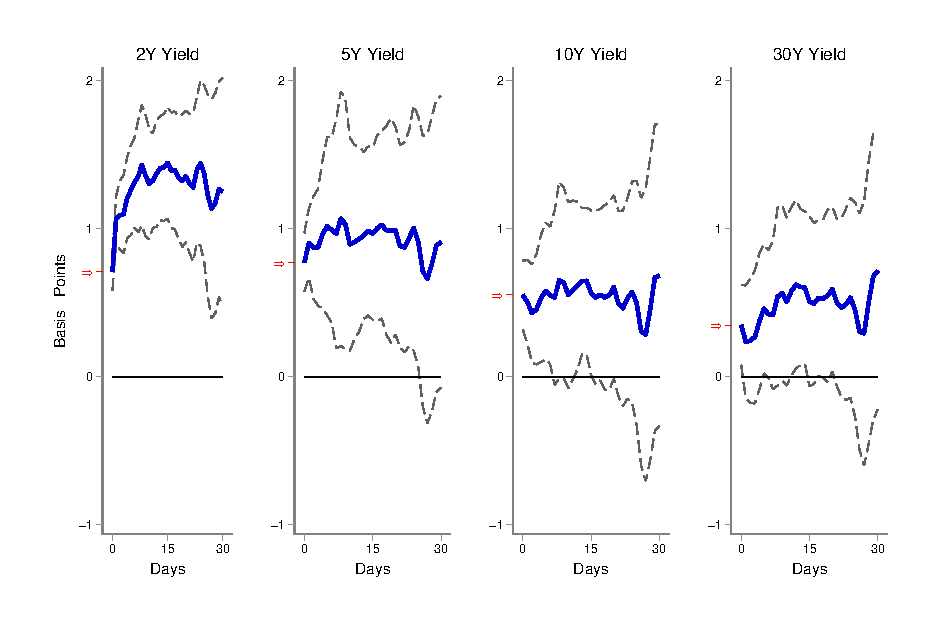
\includegraphics[trim={0.3cm 0.23cm 0.3cm 0.23cm},clip,height=0.33\textheight,width=\linewidth]{../Figures/LPs/Target/Target11YC.eps} \\
%						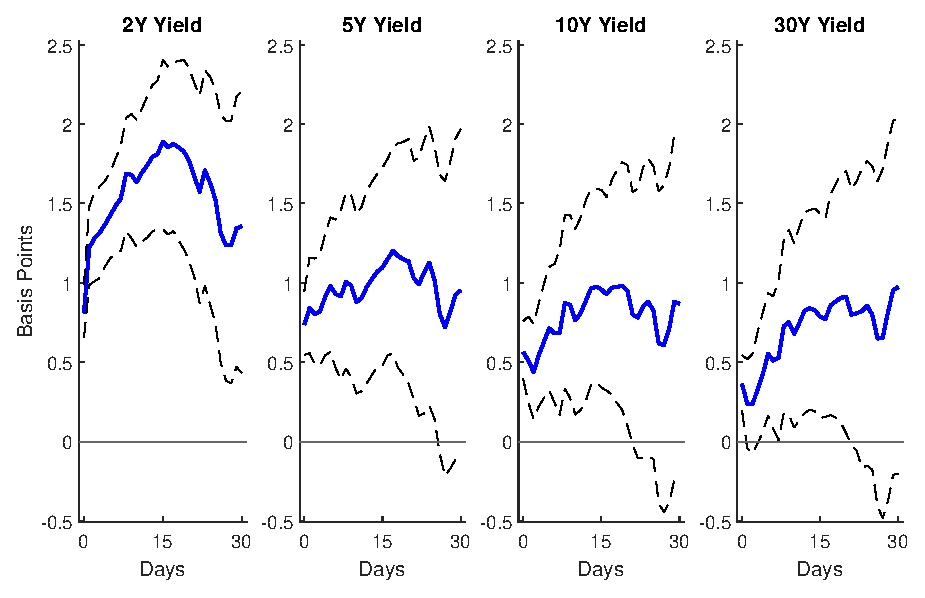
\includegraphics[trim={0.3cm 0.23cm 0.3cm 0.23cm},clip,height=0.33\textheight,width=\linewidth]{../Target/Target11YC} \\
						\vspace{-0.35cm}
						\caption{Target Surprises} \label{subfig:Target11YC}
						\vspace{0.4cm}
					\end{subfigure}
				
					\vspace{0.1cm}
					
					\begin{subfigure}[t]{\linewidth}
						\includegraphics[trim={0.3cm 0.23cm 0.3cm 0.23cm},clip,height=0.33\textheight,width=\linewidth]{../Figures/LPs/Path/Path11YC.eps} \\
%						\includegraphics[trim={0.3cm 0.23cm 0.3cm 0.23cm},clip,height=0.33\textheight,width=\linewidth]{../Path/Path11YC} \\
						\vspace{-0.35cm}
						\caption{Path Surprises} \label{subfig:Path11YC}
					\end{subfigure}
					\vspace{-0.45cm}
				\end{center}
				\fignotes{This figure plots the coefficient estimates and 95\% confidence intervals for 1 basis point target and path tightening surprises for yield changes from close of day \(t - 1\) to day \(t + \idxh\), where \(t\) is a day with a monetary policy announcement and \(\idxh = 0, 1, \ldots, 30\). An arrow in the vertical axis indicates the contemporaneous effect (when \(\idxh = 0\)). The surprises are equal to the target and path surprises (obtained with intraday data) on announcement days and zero otherwise. The sample includes all regular monetary policy announcements from January 2011 to \lastobs. The 95\% confidence bands are based on robust standard errors.}
			\end{minipage}
		\end{center}
	\end{figure}
	\end{landscape}
	}
\end{document}
% trim = {<left> <lower> <right> <upper>}

Monetary policy has a persistent effect on the yield curve. The effect of the surprises last days after an announcement. 
This post-announcement drift has been identified in advanced economies and attributed to slow-moving capital \parencite{BrooksKatzLustig:2019}. 
Big players like pension funds and foreign investors might take time to respond to the surprises. 
Section \ref{sec:flowsdypersist} provides evidence supporting this interpretation for Mexico. 

Three patterns characterize the effects of target and path surprises. 
First, the effect of path surprises at all maturities increases a few days later. Intuitively, financial markets take time to digest the implications of path surprises \parencite{GSS:2005a}. 
Second, yields respond stronger to path than to target surprises in the days following an announcement, but the effects of target surprises are more persistent. Although the need of Banxico to rely on path surprises has been low (see section \ref{sec:onimpactfx}), they have a strong impact on yields when used. 
Lastly, the persistence of the effects decreases with the maturity of the bond. Traditionally, central banks exert more control over the short end of the yield curve with conventional monetary policies. 

Overall, target and path surprises have a persistent impact on the yield curve. 

}{}	% Closes \iftoggle{fulldraft}


\section{The Effects of Monetary Policy on Portfolio Flows} \label{sec:flows}
\iftoggle{toclinks}{\gototoc}{} % Turn it on/off in packages.tex, command in macros.tex
This section shows that target and path surprises also influence portfolio flows. 
The analysis helps to understand the mechanisms behind the transmission of monetary policy. 
In particular, foreign investors play an important role in the  transmission of path surprises. 

\iftoggle{fulldraft}{					% Turn it on/off in packages.tex

\subsection{Daily Data on Portfolio Flows} \label{sec:flowsdaily}
Banxico collects daily data on the value of holdings of different types of Mexican government securities, including Treasury bills (cetes), fixed-rate bonds (bonos), floating-rate bonds (bondes) and inflation-protected bonds (udibonos). %and bonds issued by the deposit insurer (bpas). 
I focus on the bonos because they play a prominent role in the Mexican bond market \parencite{Banxico:2014}. 

The holdings data are unique because Banxico collect them daily. 
In fact, analyzing the effects of monetary policy on portfolio flows is challenging because of the frequency of the data. Cross-border capital flows (including portfolio flows, foreign direct investment, and banking flows) are reported quarterly, although some sources report portfolio flows monthly or even weekly. 
This section exploits the availability of daily data on bonos holdings to analyze how portfolio flows respond to target and path surprises. 

Banxico reports the bonos holdings of domestic and foreign investors. 
For reference, figure \ref{fig:frgnvsdmstc} compares the level of bonos and cetes holdings by residence from January 2011 to \lastobsflwbdm. 
Foreign investors were once the main players in the bonos market, they increased their holdings substantially since the bonos were included in the Citigroup's World Government Bond Index in 2010 and up to 2020,\footnote{This trend increased the liquidity premium in the bonos market \parencite{CFS:2021}.} when they reduced their exposure in response to the Covid-19 pandemic. 
Between late 2012 and early 2015, foreigners were also the main holders of cetes but rising hedging costs made short-term carry trade less attractive, which partly explains the decline since then. 

%\begin{center}
%	[Insert Figure \ref{fig:frgnvsdmstc} here.]
%\end{center}
\documentclass{article}
\usepackage{graphicx}
\usepackage[margin=1in]{geometry}
\usepackage[outdir=./]{epstopdf}  					% Avoids errors when input figures
\usepackage[labelsep=period,labelfont=bf]{caption}
%\usepackage{subcaption}
%% Personalized Macros
% Table of Contents, Tables, Subcaptions, Track Changes, Footnotes

%---------------------------------------------------------------
% Table of Contents
%---------------------------------------------------------------

% Link to ToC from section
\newcommand{\gototoc}{\vspace{-2cm} \null\hfill [\hyperlink{toc}{Go2ToC}] \newline}

% Link back to section from ToC
\newcommand{\maketoc}{
	\hypertarget{toc}{}
	\newpage
	\tableofcontents
	\vspace{2.5\bigskipamount} }

% Box with bullets for tasks to do in a section
\newenvironment{boxeditems}
	{\begin{tabular}{|p{\linewidth}|}
	\hline
	\begin{itemize}
	}
	{
	\end{itemize}
	\\ \hline
	\end{tabular} \\
	}

%---------------------------------------------------------------
% Tables
%---------------------------------------------------------------

% Estout Commands following Jörg Weber
\newcommand{\sym}[1]{\rlap{#1}}

\let\estinput=\input	% define new input command to flatten the document

\newcommand{\estauto}[2]{
	\newcolumntype{C}{>{\centering\arraybackslash}X}
	\vspace{.75ex}{
%		\begin{tabularx}{1.4\textwidth}{l*{#2}C}
		\begin{tabularx}{0.95\linewidth}{l*{#2}C}
			\toprule
			\estinput{#1}
			\\ \bottomrule
			\addlinespace[.75ex]
		\end{tabularx}
	}
}

% Allow line breaks with \\ in specialcells
\newcommand{\specialcell}[2][c]{\begin{tabular}[#1]{@{}c@{}}#2\end{tabular}}

%---------------------------------------------------------------
% Subcaptions
%---------------------------------------------------------------

% Notes after figures following Jörg Weber
\newcommand{\figtext}[1]{
	\vspace{-1ex}
	\captionsetup{justification=justified,font=footnotesize}
	\caption*{#1}
%	\captionsetup{justification=raggedright,singlelinecheck=false,font=footnotesize}
%	\caption*{\hspace{6pt}\hangindent=1.5em #1}
}

\newcommand{\fignote}[1]{\figtext{\emph{Note:~}~#1}}
\newcommand{\fignotes}[1]{\figtext{\emph{Notes:~}~#1}}

% Notes after tables
\newcommand{\tabnote}[1]{
	\begin{tablenotes}[para,flushleft]
		\footnotesize \emph{Notes:~}~#1
	\end{tablenotes}
}

%---------------------------------------------------------------
% Track Changes
%---------------------------------------------------------------

% Highlight changes in revised version with color
\newcommand{\textchange}[1]{\iftoggle{revised}{\textcolor{blue}{#1}}{#1}}

%---------------------------------------------------------------
% Footnotes
%---------------------------------------------------------------

%% Change the look of foonote indicators
%\makeatletter
%\let \@makefntextorig \@makefntext
%\newcommand{\@makefntextcustom}[1]{%
%	\thefootnote.\enskip #1%
%}
%\renewcommand{\@makefntext}[1]{\@makefntextcustom{#1}}
%\makeatother
%
%% Change the look of endnote indicators
%\renewcommand{\makeenmark}{\hbox{$^{\theenmark}$}}
%\makeatletter
%\def\enoteformat{%
%	\rightskip\z@ \leftskip\z@ \parindent=1.8em
%	\leavevmode{\setbox\z@=\lastbox}\llap{\theenmark.\enskip}%
%}
%\makeatother			% Personalized commands
%% Personalized Macros
% Variable Definitions, Equations

%---------------------------------------------------------------
% Variable Definitions
%---------------------------------------------------------------
\providecommand{\tiie}{TIIE28D}
\providecommand{\lastobs}{December 2021}
\providecommand{\lastobsfx}{November 2021}
\providecommand{\lastobsflwbdm}{December 2021}
\providecommand{\lastobsflwtic}{August 2021}
\providecommand{\idxt}{t}
\providecommand{\idxh}{h}
\providecommand{\idxi}{i}
\providecommand{\idxsfwd}{\idxt+\idxh}
\providecommand{\idxslag}{\idxt-1}
\providecommand{\yld}{y}
\providecommand{\ctrls}{z}
\providecommand{\hld}{H}
\providecommand{\depvar}{\Delta \yld_{\idxt}}
\providecommand{\mps}{\Delta x_{\idxt}}
\providecommand{\depvarclean}{\depvar^{*}}
\providecommand{\mpsclean}{\mps^{*}}
\providecommand{\paramB}{\beta}
\providecommand{\intrcpt}{\paramB_{0}}
\providecommand{\slopetrgt}{\paramB_{1}}
\providecommand{\slopepath}{\paramB_{2}}
\providecommand{\assets}{X}
\providecommand{\factors}{F}
\providecommand{\loadings}{\Lambda}
\providecommand{\rotated}{Z}
\providecommand{\rmatrix}{U}
\providecommand{\rtdone}{\rotated_{1}}
\providecommand{\rtdtwo}{\rotated_{2}}
\providecommand{\rtdonereg}{Target_{\idxt}}
\providecommand{\rtdtworeg}{Path_{\idxt}}
\providecommand{\lagidx}{j}
\providecommand{\lagorder}{p}
\providecommand{\lagparam}{\gamma}   %\alpha
\providecommand{\lagoper}{L}
\providecommand{\depvarflw}{\Delta \hld_{\idxt}}
\providecommand{\flows}{w_{\idxt}}
\providecommand{\flowslag}{w_{\idxt - \lagidx}}
\providecommand{\lagsum}{\sum_{\lagidx = 1}^{\lagorder} \lagparam_{\lagidx} \flowslag}
\providecommand{\lagsumh}{\sum_{\lagidx = 1}^{\lagorder} \lagparam^{\lagidx}_\idxh \flowslag}
\providecommand{\dimobs}{T}
\providecommand{\dimassets}{n}
\providecommand{\dimfactors}{k}
\providecommand{\dimnull}{\dimfactors_{0}}
\providecommand{\dimsassets}{\dimobs \times \dimassets}
\providecommand{\dimsfactors}{\dimobs \times \dimfactors}
\providecommand{\dimsloadings}{\dimfactors \times \dimassets}
\providecommand{\errorreg}{\varepsilon_{\idxt}}
\providecommand{\errorfac}{\zeta}
\providecommand{\errorflows}{\nu_{\idxt}}
\providecommand{\Rsqrt}{R^{2}}

\providecommand{\dpv}{y}
\providecommand{\idv}{x}
\providecommand{\omv}{\omega}
\providecommand{\dpvstar}{\dpv^{*}}
\providecommand{\idvstar}{\idv^{*}}
\providecommand{\jobs}{Jobs}
\providecommand{\errortrue}{\varepsilon}
\providecommand{\errormix}{\tau}
\providecommand{\melhs}{\nu}
\providecommand{\merhs}{u}
\providecommand{\mean}{\mu}
\providecommand{\covar}{\sigma}
\providecommand{\corr}{\rho}
\providecommand{\var}{\covar^{2}}
\providecommand{\meanE}{\mean_{\errortrue}}
\providecommand{\meanU}{\mean_{\merhs}}
\providecommand{\meanV}{\mean_{\melhs}}
\providecommand{\varE}{\var_{\errortrue}}
\providecommand{\varU}{\var_{\merhs}}
\providecommand{\varV}{\var_{\melhs}}
\providecommand{\varX}{\var_{\idv}}
\providecommand{\varXstar}{\var_{\idvstar}}
\providecommand{\covarEX}{\covar_{\errortrue \idvstar}}
\providecommand{\covarUE}{\covar_{\merhs \errortrue}}
\providecommand{\covarVE}{\covar_{\melhs \errortrue}}
\providecommand{\covarUX}{\covar_{\merhs \idvstar}}
\providecommand{\covarUY}{\covar_{\merhs \dpvstar}}
\providecommand{\covarVX}{\covar_{\melhs \idvstar}}
\providecommand{\covarVY}{\covar_{\melhs \dpvstar}}
\providecommand{\covarUV}{\covar_{\merhs \melhs}}
\providecommand{\covarWXe}{\covar_{\omv \idv}}
\providecommand{\covarVXe}{\covar_{\melhs \idv}}
\providecommand{\corrUV}{\corr_{\merhs \melhs}}
\providecommand{\corrUX}{\corr_{\merhs \idvstar}}
\providecommand{\corrUY}{\corr_{\merhs \dpvstar}}
\providecommand{\corrVX}{\corr_{\melhs \idvstar}}
\providecommand{\corrVY}{\corr_{\melhs \dpvstar}}
\providecommand{\paramG}{\gamma}
\providecommand{\estimB}{\hat{\paramB}}
\providecommand{\paramSE}{\varE}
\providecommand{\estimSE}{\hat{\paramSE}}
\providecommand{\paramAVB}{s}
\providecommand{\estimAVB}{\hat{\paramAVB}}
\providecommand{\attnfactor}{\lambda}
\providecommand{\plim}{\mathrm{plim}}

\providecommand{\reg}{\delta}
\providecommand{\regVonX}{\reg_{\melhs \idv}}
\providecommand{\regWonX}{\reg_{\omv \idv}}
\providecommand{\regWonXstar}{\reg_{\omv \idvstar}}

%---------------------------------------------------------------
% Equations
%---------------------------------------------------------------
\newcommand{\eqOneFac}{\depvar = \intrcpt + \slopetrgt \mps + \errorreg}
\newcommand{\eqOneFacOV}{\depvar = \intrcpt + \slopetrgt PRS_{\idxt} + \paramB_{2} \Delta VIX_{\idxt} + \paramB_{3} \Delta USY_{\idxt} + \paramB_{4} WTI_{\idxt} + \paramB_{5} \jobs_{\idxt} + \errorreg}
\newcommand{\eqTwoFacP}{\depvar = \intrcpt + \slopetrgt \rtdonereg + \slopepath \rtdtworeg + \errorreg}
\newcommand{\eqTwoFacF}{\depvarflw = \intrcpt + \slopetrgt \rtdonereg + \slopepath \rtdtworeg + \errorreg}
\newcommand{\eqPCA}{\assets = \factors \loadings + \errorfac}
\newcommand{\eqRotation}{\rotated = \factors \, \rmatrix}
\newcommand{\eqFlows}{\flows = \intrcpt + \slopetrgt \rtdonereg + \slopepath \rtdtworeg + \lagsum + \eta^{'} \ctrls_{\idxslag} + \errorflows}
%\newcommand{\eqLagPoly}{\lagsum = 1 - \lagparam_{1} \lagoper - \lagparam_{2} \lagoper^{2} - \ldots - \lagparam_{\lagorder} \lagoper^{\lagorder}}
\newcommand{\eqAsym}{\yld_{\idxt} = \intrcpt + \paramB_{1} \rtdonereg \mathds{1} \left(\rtdonereg > 0 \right) + \paramB_{2} \rtdonereg \mathds{1} \left(\rtdonereg < 0 \right) \\ + \paramB_{3} \rtdtworeg \mathds{1} \left(\rtdtworeg > 0 \right) + \paramB_{4} \rtdtworeg \mathds{1} \left(\rtdtworeg < 0 \right) + \errorreg}

\newcommand{\eqDGP}{\dpvstar &= \paramB \idvstar + \errortrue}
\newcommand{\eqDGPme}{\dpv = \paramB \idv + \errormix = \paramB \idv + \eqErrormix}
\newcommand{\eqDGPov}{\dpvstar = \paramB \idvstar + \paramG \omv +  \errortrue}
\newcommand{\eqMEdpv}{\dpv &= \dpvstar + \melhs}
\newcommand{\eqMEidv}{\idv &= \idvstar + \merhs}
\newcommand{\eqAtten}{\attnfactor = \frac{\varXstar}{\varXstar + \varU}}
\newcommand{\eqAttenInLine}{\attnfactor = \varXstar / \left(\varXstar + \varU\right) }
\newcommand{\eqErrormix}{\errortrue - \paramB \merhs + \melhs}

\newcommand{\eqPlimBstd}{\plim \left( \estimB \right) = \frac{cov(\idv, \dpvstar)}{var(\idv)} = \frac{cov(\idvstar + \merhs, \paramB \idvstar + \errortrue)}{var(\idvstar + \merhs)} = \paramB \frac{\varXstar}{\varXstar + \varU} = \paramB \attnfactor}
\newcommand{\eqPlimBstdshort}{\plim (\estimB) = \paramB \attnfactor}

%\newcommand{\eqPlimSstd}{\plim \left( \estimAVB \right) = \plim \left( \frac{\estimSE}{\hat{\varX}} \right) = \frac{\varE + (1-\attnfactor)^{2} \paramB^{2} \varXstar + \attnfactor^{2} \paramB^{2} \varU}{\varXstar + \varU} = \attnfactor \paramAVB + \attnfactor(1 - \attnfactor) \paramB^{2}}
\newcommand{\eqPlimSstd}{\plim \left( \estimAVB \right) = \attnfactor \paramAVB + \attnfactor(1 - \attnfactor) \paramB^{2}}

\newcommand{\eqPlimBnew}{\plim \left( \estimB \right) 
	= \frac{cov(\idv, \dpv)}{var(\idv)} 
	= \frac{cov(\idvstar + \merhs, \paramB \idvstar + \paramG \omv + \errortrue)}{var(\idvstar + \merhs)} 
	= \frac{\paramB \varXstar + \paramG \covarWXe}{\varXstar + \varU}  }

\newcommand{\eqPlimBbias}{\plim \left( \estimB \right)
	= \paramB \frac{\varXstar}{\varX} + \paramG \frac{\covarWXe}{\varX}
	= \paramB \attnfactor + \paramG \regWonX}

\providecommand{\errordepvar}{e_{y}}
\providecommand{\errormps}{e_{x}}
\newcommand{\eqMEdepvar}{\depvar &= \depvarclean + \errordepvar}
\newcommand{\eqMEmps}{\mps &= \mpsclean + \errormps}

\newcommand{\eqLPrhs}{\alpha_{\idxh} + \beta^{1}_{\idxh} \; \rtdonereg +  \beta^{2}_{\idxh} \; \rtdtworeg + \eta^{'}_{\idxh} \ctrls_{\idxslag}  + u_{\idxsfwd}}

\newcommand{\eqLPprices}{\yld_{\idxsfwd} - \yld_{\idxslag} = \eqLPrhs} 

\newcommand{\eqLPflows}{\hld_{\idxsfwd} - \hld_{\idxslag} = \eqLPrhs} 
% \gamma_{\idxh} \Delta \yld_{\idxslag} 
%\alpha_{\idxh} + \beta^{1}_{\idxh} \; \rtdonereg +  \beta^{2}_{\idxh} \; \rtdtworeg + \lagsumh + \eta_{\idxh} \ctrls_{\idxslag}  + u_{\idxsfwd}

\newcommand{\eqLP}{\yld_{\idxsfwd} - \yld_{\idxslag} = \alpha_{\idxh} + \gamma_{\idxh} \mps + u_{\idxsfwd}} 			    % Personalized commands

\begin{document}
	\begin{figure}[!htb]
		\caption{Holdings of Cetes and Bonos by Nationality} \label{fig:frgnvsdmstc}
		\begin{center}								% center the minipage on the line
			\begin{minipage}{0.9\linewidth}
%				\vspace{-0.4cm}
				\begin{center}							% center the figure inside the minipage
					\includegraphics[width=1\textwidth,height=.3\textheight]{../Figures/Flows/frgnvsdmstc} \\
%					\includegraphics[width=1\textwidth,height=.3\textheight]{frgnvsdmstc} \\
				\end{center}
%				\vspace{-0.4cm}
				\fignotes{This figure shows the net holdings of Mexican Treasury bills (cetes) and fixed-rate sovereign bonds (bonos) by investor nationality from January 2011 to \lastobsflwbdm.}
			\end{minipage}
		\end{center}
	\end{figure}
\end{document}
% trim = {<left> <lower> <right> <upper>}

Banxico categorizes domestic investors into banks, mutual funds, pension funds, insurers and non-financial investors (firms and households). 
Figure \ref{fig:bndgroups} displays the level of bonos holdings by domestic residents. 
Pension funds are key players in the bonos market, but recently non-financial investors and banks started accumulating a larger share of bonos. 
On the other hand, insurers and mutual funds maintain the smallest share of the market. 
In Mexico, insurers usually hold bonos to maturity, and most of the mutual funds are shot-term debt funds with highly liquid investments.

%\begin{center}
%	[Insert Figure \ref{fig:bndgroups} here.]
%\end{center}
\documentclass{article}
\usepackage{graphicx}
\usepackage[margin=1in]{geometry}
\usepackage[outdir=./]{epstopdf}  					% Avoids errors when input figures
\usepackage[labelsep=period,labelfont=bf]{caption}
%\usepackage{subcaption}
%% Personalized Macros
% Table of Contents, Tables, Subcaptions, Track Changes, Footnotes

%---------------------------------------------------------------
% Table of Contents
%---------------------------------------------------------------

% Link to ToC from section
\newcommand{\gototoc}{\vspace{-2cm} \null\hfill [\hyperlink{toc}{Go2ToC}] \newline}

% Link back to section from ToC
\newcommand{\maketoc}{
	\hypertarget{toc}{}
	\newpage
	\tableofcontents
	\vspace{2.5\bigskipamount} }

% Box with bullets for tasks to do in a section
\newenvironment{boxeditems}
	{\begin{tabular}{|p{\linewidth}|}
	\hline
	\begin{itemize}
	}
	{
	\end{itemize}
	\\ \hline
	\end{tabular} \\
	}

%---------------------------------------------------------------
% Tables
%---------------------------------------------------------------

% Estout Commands following Jörg Weber
\newcommand{\sym}[1]{\rlap{#1}}

\let\estinput=\input	% define new input command to flatten the document

\newcommand{\estauto}[2]{
	\newcolumntype{C}{>{\centering\arraybackslash}X}
	\vspace{.75ex}{
%		\begin{tabularx}{1.4\textwidth}{l*{#2}C}
		\begin{tabularx}{0.95\linewidth}{l*{#2}C}
			\toprule
			\estinput{#1}
			\\ \bottomrule
			\addlinespace[.75ex]
		\end{tabularx}
	}
}

% Allow line breaks with \\ in specialcells
\newcommand{\specialcell}[2][c]{\begin{tabular}[#1]{@{}c@{}}#2\end{tabular}}

%---------------------------------------------------------------
% Subcaptions
%---------------------------------------------------------------

% Notes after figures following Jörg Weber
\newcommand{\figtext}[1]{
	\vspace{-1ex}
	\captionsetup{justification=justified,font=footnotesize}
	\caption*{#1}
%	\captionsetup{justification=raggedright,singlelinecheck=false,font=footnotesize}
%	\caption*{\hspace{6pt}\hangindent=1.5em #1}
}

\newcommand{\fignote}[1]{\figtext{\emph{Note:~}~#1}}
\newcommand{\fignotes}[1]{\figtext{\emph{Notes:~}~#1}}

% Notes after tables
\newcommand{\tabnote}[1]{
	\begin{tablenotes}[para,flushleft]
		\footnotesize \emph{Notes:~}~#1
	\end{tablenotes}
}

%---------------------------------------------------------------
% Track Changes
%---------------------------------------------------------------

% Highlight changes in revised version with color
\newcommand{\textchange}[1]{\iftoggle{revised}{\textcolor{blue}{#1}}{#1}}

%---------------------------------------------------------------
% Footnotes
%---------------------------------------------------------------

%% Change the look of foonote indicators
%\makeatletter
%\let \@makefntextorig \@makefntext
%\newcommand{\@makefntextcustom}[1]{%
%	\thefootnote.\enskip #1%
%}
%\renewcommand{\@makefntext}[1]{\@makefntextcustom{#1}}
%\makeatother
%
%% Change the look of endnote indicators
%\renewcommand{\makeenmark}{\hbox{$^{\theenmark}$}}
%\makeatletter
%\def\enoteformat{%
%	\rightskip\z@ \leftskip\z@ \parindent=1.8em
%	\leavevmode{\setbox\z@=\lastbox}\llap{\theenmark.\enskip}%
%}
%\makeatother			% Personalized commands
%% Personalized Macros
% Variable Definitions, Equations

%---------------------------------------------------------------
% Variable Definitions
%---------------------------------------------------------------
\providecommand{\tiie}{TIIE28D}
\providecommand{\lastobs}{December 2021}
\providecommand{\lastobsfx}{November 2021}
\providecommand{\lastobsflwbdm}{December 2021}
\providecommand{\lastobsflwtic}{August 2021}
\providecommand{\idxt}{t}
\providecommand{\idxh}{h}
\providecommand{\idxi}{i}
\providecommand{\idxsfwd}{\idxt+\idxh}
\providecommand{\idxslag}{\idxt-1}
\providecommand{\yld}{y}
\providecommand{\ctrls}{z}
\providecommand{\hld}{H}
\providecommand{\depvar}{\Delta \yld_{\idxt}}
\providecommand{\mps}{\Delta x_{\idxt}}
\providecommand{\depvarclean}{\depvar^{*}}
\providecommand{\mpsclean}{\mps^{*}}
\providecommand{\paramB}{\beta}
\providecommand{\intrcpt}{\paramB_{0}}
\providecommand{\slopetrgt}{\paramB_{1}}
\providecommand{\slopepath}{\paramB_{2}}
\providecommand{\assets}{X}
\providecommand{\factors}{F}
\providecommand{\loadings}{\Lambda}
\providecommand{\rotated}{Z}
\providecommand{\rmatrix}{U}
\providecommand{\rtdone}{\rotated_{1}}
\providecommand{\rtdtwo}{\rotated_{2}}
\providecommand{\rtdonereg}{Target_{\idxt}}
\providecommand{\rtdtworeg}{Path_{\idxt}}
\providecommand{\lagidx}{j}
\providecommand{\lagorder}{p}
\providecommand{\lagparam}{\gamma}   %\alpha
\providecommand{\lagoper}{L}
\providecommand{\depvarflw}{\Delta \hld_{\idxt}}
\providecommand{\flows}{w_{\idxt}}
\providecommand{\flowslag}{w_{\idxt - \lagidx}}
\providecommand{\lagsum}{\sum_{\lagidx = 1}^{\lagorder} \lagparam_{\lagidx} \flowslag}
\providecommand{\lagsumh}{\sum_{\lagidx = 1}^{\lagorder} \lagparam^{\lagidx}_\idxh \flowslag}
\providecommand{\dimobs}{T}
\providecommand{\dimassets}{n}
\providecommand{\dimfactors}{k}
\providecommand{\dimnull}{\dimfactors_{0}}
\providecommand{\dimsassets}{\dimobs \times \dimassets}
\providecommand{\dimsfactors}{\dimobs \times \dimfactors}
\providecommand{\dimsloadings}{\dimfactors \times \dimassets}
\providecommand{\errorreg}{\varepsilon_{\idxt}}
\providecommand{\errorfac}{\zeta}
\providecommand{\errorflows}{\nu_{\idxt}}
\providecommand{\Rsqrt}{R^{2}}

\providecommand{\dpv}{y}
\providecommand{\idv}{x}
\providecommand{\omv}{\omega}
\providecommand{\dpvstar}{\dpv^{*}}
\providecommand{\idvstar}{\idv^{*}}
\providecommand{\jobs}{Jobs}
\providecommand{\errortrue}{\varepsilon}
\providecommand{\errormix}{\tau}
\providecommand{\melhs}{\nu}
\providecommand{\merhs}{u}
\providecommand{\mean}{\mu}
\providecommand{\covar}{\sigma}
\providecommand{\corr}{\rho}
\providecommand{\var}{\covar^{2}}
\providecommand{\meanE}{\mean_{\errortrue}}
\providecommand{\meanU}{\mean_{\merhs}}
\providecommand{\meanV}{\mean_{\melhs}}
\providecommand{\varE}{\var_{\errortrue}}
\providecommand{\varU}{\var_{\merhs}}
\providecommand{\varV}{\var_{\melhs}}
\providecommand{\varX}{\var_{\idv}}
\providecommand{\varXstar}{\var_{\idvstar}}
\providecommand{\covarEX}{\covar_{\errortrue \idvstar}}
\providecommand{\covarUE}{\covar_{\merhs \errortrue}}
\providecommand{\covarVE}{\covar_{\melhs \errortrue}}
\providecommand{\covarUX}{\covar_{\merhs \idvstar}}
\providecommand{\covarUY}{\covar_{\merhs \dpvstar}}
\providecommand{\covarVX}{\covar_{\melhs \idvstar}}
\providecommand{\covarVY}{\covar_{\melhs \dpvstar}}
\providecommand{\covarUV}{\covar_{\merhs \melhs}}
\providecommand{\covarWXe}{\covar_{\omv \idv}}
\providecommand{\covarVXe}{\covar_{\melhs \idv}}
\providecommand{\corrUV}{\corr_{\merhs \melhs}}
\providecommand{\corrUX}{\corr_{\merhs \idvstar}}
\providecommand{\corrUY}{\corr_{\merhs \dpvstar}}
\providecommand{\corrVX}{\corr_{\melhs \idvstar}}
\providecommand{\corrVY}{\corr_{\melhs \dpvstar}}
\providecommand{\paramG}{\gamma}
\providecommand{\estimB}{\hat{\paramB}}
\providecommand{\paramSE}{\varE}
\providecommand{\estimSE}{\hat{\paramSE}}
\providecommand{\paramAVB}{s}
\providecommand{\estimAVB}{\hat{\paramAVB}}
\providecommand{\attnfactor}{\lambda}
\providecommand{\plim}{\mathrm{plim}}

\providecommand{\reg}{\delta}
\providecommand{\regVonX}{\reg_{\melhs \idv}}
\providecommand{\regWonX}{\reg_{\omv \idv}}
\providecommand{\regWonXstar}{\reg_{\omv \idvstar}}

%---------------------------------------------------------------
% Equations
%---------------------------------------------------------------
\newcommand{\eqOneFac}{\depvar = \intrcpt + \slopetrgt \mps + \errorreg}
\newcommand{\eqOneFacOV}{\depvar = \intrcpt + \slopetrgt PRS_{\idxt} + \paramB_{2} \Delta VIX_{\idxt} + \paramB_{3} \Delta USY_{\idxt} + \paramB_{4} WTI_{\idxt} + \paramB_{5} \jobs_{\idxt} + \errorreg}
\newcommand{\eqTwoFacP}{\depvar = \intrcpt + \slopetrgt \rtdonereg + \slopepath \rtdtworeg + \errorreg}
\newcommand{\eqTwoFacF}{\depvarflw = \intrcpt + \slopetrgt \rtdonereg + \slopepath \rtdtworeg + \errorreg}
\newcommand{\eqPCA}{\assets = \factors \loadings + \errorfac}
\newcommand{\eqRotation}{\rotated = \factors \, \rmatrix}
\newcommand{\eqFlows}{\flows = \intrcpt + \slopetrgt \rtdonereg + \slopepath \rtdtworeg + \lagsum + \eta^{'} \ctrls_{\idxslag} + \errorflows}
%\newcommand{\eqLagPoly}{\lagsum = 1 - \lagparam_{1} \lagoper - \lagparam_{2} \lagoper^{2} - \ldots - \lagparam_{\lagorder} \lagoper^{\lagorder}}
\newcommand{\eqAsym}{\yld_{\idxt} = \intrcpt + \paramB_{1} \rtdonereg \mathds{1} \left(\rtdonereg > 0 \right) + \paramB_{2} \rtdonereg \mathds{1} \left(\rtdonereg < 0 \right) \\ + \paramB_{3} \rtdtworeg \mathds{1} \left(\rtdtworeg > 0 \right) + \paramB_{4} \rtdtworeg \mathds{1} \left(\rtdtworeg < 0 \right) + \errorreg}

\newcommand{\eqDGP}{\dpvstar &= \paramB \idvstar + \errortrue}
\newcommand{\eqDGPme}{\dpv = \paramB \idv + \errormix = \paramB \idv + \eqErrormix}
\newcommand{\eqDGPov}{\dpvstar = \paramB \idvstar + \paramG \omv +  \errortrue}
\newcommand{\eqMEdpv}{\dpv &= \dpvstar + \melhs}
\newcommand{\eqMEidv}{\idv &= \idvstar + \merhs}
\newcommand{\eqAtten}{\attnfactor = \frac{\varXstar}{\varXstar + \varU}}
\newcommand{\eqAttenInLine}{\attnfactor = \varXstar / \left(\varXstar + \varU\right) }
\newcommand{\eqErrormix}{\errortrue - \paramB \merhs + \melhs}

\newcommand{\eqPlimBstd}{\plim \left( \estimB \right) = \frac{cov(\idv, \dpvstar)}{var(\idv)} = \frac{cov(\idvstar + \merhs, \paramB \idvstar + \errortrue)}{var(\idvstar + \merhs)} = \paramB \frac{\varXstar}{\varXstar + \varU} = \paramB \attnfactor}
\newcommand{\eqPlimBstdshort}{\plim (\estimB) = \paramB \attnfactor}

%\newcommand{\eqPlimSstd}{\plim \left( \estimAVB \right) = \plim \left( \frac{\estimSE}{\hat{\varX}} \right) = \frac{\varE + (1-\attnfactor)^{2} \paramB^{2} \varXstar + \attnfactor^{2} \paramB^{2} \varU}{\varXstar + \varU} = \attnfactor \paramAVB + \attnfactor(1 - \attnfactor) \paramB^{2}}
\newcommand{\eqPlimSstd}{\plim \left( \estimAVB \right) = \attnfactor \paramAVB + \attnfactor(1 - \attnfactor) \paramB^{2}}

\newcommand{\eqPlimBnew}{\plim \left( \estimB \right) 
	= \frac{cov(\idv, \dpv)}{var(\idv)} 
	= \frac{cov(\idvstar + \merhs, \paramB \idvstar + \paramG \omv + \errortrue)}{var(\idvstar + \merhs)} 
	= \frac{\paramB \varXstar + \paramG \covarWXe}{\varXstar + \varU}  }

\newcommand{\eqPlimBbias}{\plim \left( \estimB \right)
	= \paramB \frac{\varXstar}{\varX} + \paramG \frac{\covarWXe}{\varX}
	= \paramB \attnfactor + \paramG \regWonX}

\providecommand{\errordepvar}{e_{y}}
\providecommand{\errormps}{e_{x}}
\newcommand{\eqMEdepvar}{\depvar &= \depvarclean + \errordepvar}
\newcommand{\eqMEmps}{\mps &= \mpsclean + \errormps}

\newcommand{\eqLPrhs}{\alpha_{\idxh} + \beta^{1}_{\idxh} \; \rtdonereg +  \beta^{2}_{\idxh} \; \rtdtworeg + \eta^{'}_{\idxh} \ctrls_{\idxslag}  + u_{\idxsfwd}}

\newcommand{\eqLPprices}{\yld_{\idxsfwd} - \yld_{\idxslag} = \eqLPrhs} 

\newcommand{\eqLPflows}{\hld_{\idxsfwd} - \hld_{\idxslag} = \eqLPrhs} 
% \gamma_{\idxh} \Delta \yld_{\idxslag} 
%\alpha_{\idxh} + \beta^{1}_{\idxh} \; \rtdonereg +  \beta^{2}_{\idxh} \; \rtdtworeg + \lagsumh + \eta_{\idxh} \ctrls_{\idxslag}  + u_{\idxsfwd}

\newcommand{\eqLP}{\yld_{\idxsfwd} - \yld_{\idxslag} = \alpha_{\idxh} + \gamma_{\idxh} \mps + u_{\idxsfwd}} 			    % Personalized commands

\begin{document}
	\begin{figure}[!htb]
		\caption{Holdings of Bonos by Type of Investor} \label{fig:bndgroups}
		\begin{center}								% center the minipage on the line
			\begin{minipage}{0.9\linewidth}
%				\vspace{-0.4cm}
				\begin{center}							% center the figure inside the minipage
					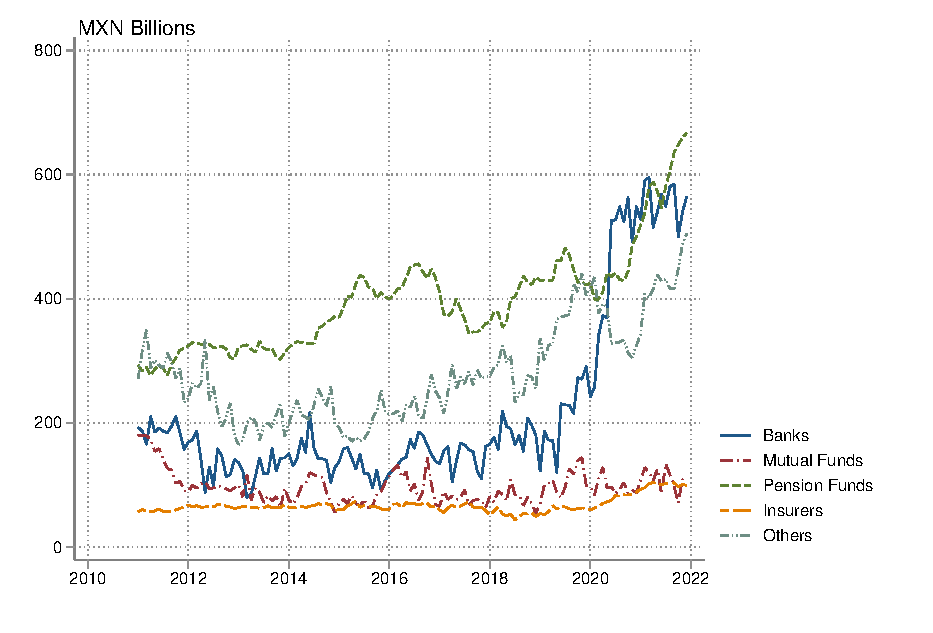
\includegraphics[width=1\textwidth,height=.3\textheight]{../Figures/Flows/bndgroups} \\
				\end{center}
%				\vspace{-0.4cm}
				\fignotes{This figure shows the net holdings of fixed-rate Mexican sovereign bonds (bonos) by type of domestic investor from January 2011 to \lastobsflwbdm.}
			\end{minipage}
		\end{center}
	\end{figure}
\end{document}
% trim = {<left> <lower> <right> <upper>}

The holdings data need to be adjusted for valuation effects. %distinguish between valuation changes and net purchases of bonos before using the data. 
Changes in the nominal value of bonos holdings can reflect a change in the amount of bonos and/or a change in the value of the bonos. 
Therefore, I deflate the nominal value of bonos holdings with a rate equal to the percentage change in the price.
The daily percentage change in the price of the bonos is approximated as minus the duration times the daily change in the yield. 
The duration of the bonos is calculated using the par yields from the Bloomberg Fair Value (BFV) curve for Mexico and the average maturity of the bonos reported by Banxico.\footnote{The change in the log price of the bond, \(\mathrm{d}\log (P)\), is approximately equal to \(- D_{mod} \times \mathrm{d} y\), in which \(D_{mod}\) is the modified duration and \(\mathrm{d} y\) is the change in the yield. Each day, the BFV yield closest to the average maturity is used to calculate \(D_{mod}\) and \(\mathrm{d} y\). Banxico reports every month the average maturity (expressed in days) of the bonos outstanding. For the adjustment, the average maturity is expressed in years and rounded to the nearest integer; the same value is used for all the days in a month.} 
In this way, a change in the deflated value of bonos holdings only reflects a change in the amount of bonos regardless of price movements. 
This information on net purchases is then used to analyze the effects of monetary policy on portfolio flows. 
Although the adjustment is far from perfect, it is reasonable given the available data; for instance, the average maturity data is not broken down by tenor or by type of investor. Fortunately, %most changes in yields are usually parallel
the adjustment does not alter the conclusions as the next section shows. 


\subsection{Contemporaneous Effects} \label{sec:onimpactflows}
Similar to the case of asset prices, the following event-study regression quantifies the on-impact effects of target and path surprises on the flows of bonos: 
\begin{equation} \label{eq:nTwoFacF}
	\eqTwoFacF ,
\end{equation}	%(\ref{eq:nTwoFacF})
\noindent in which \(\depvarflw\) is the daily change in the (deflated) value of bonos holdings (i.e., the flows) by type of investor around monetary policy announcements. 
The rest is similar to equation (\ref{eq:nTwoFacP}). 
Table \ref{tab:fctrsbndid} reports the results.

%\begin{center}
%	[Insert Table \ref{tab:fctrsbndid} here.]
%\end{center}
\documentclass[a4paper,12pt]{article}
\usepackage[labelsep=period,labelfont=bf]{caption}
\usepackage{multirow}
\usepackage{booktabs}
\usepackage{threeparttable}
\usepackage{pdflscape}
\usepackage{tabularx}
\usepackage{afterpage}
%\usepackage[margin=1in]{geometry}
%%% Personalized Macros
% Table of Contents, Tables, Subcaptions, Track Changes, Footnotes

%---------------------------------------------------------------
% Table of Contents
%---------------------------------------------------------------

% Link to ToC from section
\newcommand{\gototoc}{\vspace{-2cm} \null\hfill [\hyperlink{toc}{Go2ToC}] \newline}

% Link back to section from ToC
\newcommand{\maketoc}{
	\hypertarget{toc}{}
	\newpage
	\tableofcontents
	\vspace{2.5\bigskipamount} }

% Box with bullets for tasks to do in a section
\newenvironment{boxeditems}
	{\begin{tabular}{|p{\linewidth}|}
	\hline
	\begin{itemize}
	}
	{
	\end{itemize}
	\\ \hline
	\end{tabular} \\
	}

%---------------------------------------------------------------
% Tables
%---------------------------------------------------------------

% Estout Commands following Jörg Weber
\newcommand{\sym}[1]{\rlap{#1}}

\let\estinput=\input	% define new input command to flatten the document

\newcommand{\estauto}[2]{
	\newcolumntype{C}{>{\centering\arraybackslash}X}
	\vspace{.75ex}{
%		\begin{tabularx}{1.4\textwidth}{l*{#2}C}
		\begin{tabularx}{0.95\linewidth}{l*{#2}C}
			\toprule
			\estinput{#1}
			\\ \bottomrule
			\addlinespace[.75ex]
		\end{tabularx}
	}
}

% Allow line breaks with \\ in specialcells
\newcommand{\specialcell}[2][c]{\begin{tabular}[#1]{@{}c@{}}#2\end{tabular}}

%---------------------------------------------------------------
% Subcaptions
%---------------------------------------------------------------

% Notes after figures following Jörg Weber
\newcommand{\figtext}[1]{
	\vspace{-1ex}
	\captionsetup{justification=justified,font=footnotesize}
	\caption*{#1}
%	\captionsetup{justification=raggedright,singlelinecheck=false,font=footnotesize}
%	\caption*{\hspace{6pt}\hangindent=1.5em #1}
}

\newcommand{\fignote}[1]{\figtext{\emph{Note:~}~#1}}
\newcommand{\fignotes}[1]{\figtext{\emph{Notes:~}~#1}}

% Notes after tables
\newcommand{\tabnote}[1]{
	\begin{tablenotes}[para,flushleft]
		\footnotesize \emph{Notes:~}~#1
	\end{tablenotes}
}

%---------------------------------------------------------------
% Track Changes
%---------------------------------------------------------------

% Highlight changes in revised version with color
\newcommand{\textchange}[1]{\iftoggle{revised}{\textcolor{blue}{#1}}{#1}}

%---------------------------------------------------------------
% Footnotes
%---------------------------------------------------------------

%% Change the look of foonote indicators
%\makeatletter
%\let \@makefntextorig \@makefntext
%\newcommand{\@makefntextcustom}[1]{%
%	\thefootnote.\enskip #1%
%}
%\renewcommand{\@makefntext}[1]{\@makefntextcustom{#1}}
%\makeatother
%
%% Change the look of endnote indicators
%\renewcommand{\makeenmark}{\hbox{$^{\theenmark}$}}
%\makeatletter
%\def\enoteformat{%
%	\rightskip\z@ \leftskip\z@ \parindent=1.8em
%	\leavevmode{\setbox\z@=\lastbox}\llap{\theenmark.\enskip}%
%}
%\makeatother			% Personalized commands
%%% Personalized Macros
% Variable Definitions, Equations

%---------------------------------------------------------------
% Variable Definitions
%---------------------------------------------------------------
\providecommand{\tiie}{TIIE28D}
\providecommand{\lastobs}{December 2021}
\providecommand{\lastobsfx}{November 2021}
\providecommand{\lastobsflwbdm}{December 2021}
\providecommand{\lastobsflwtic}{August 2021}
\providecommand{\idxt}{t}
\providecommand{\idxh}{h}
\providecommand{\idxi}{i}
\providecommand{\idxsfwd}{\idxt+\idxh}
\providecommand{\idxslag}{\idxt-1}
\providecommand{\yld}{y}
\providecommand{\ctrls}{z}
\providecommand{\hld}{H}
\providecommand{\depvar}{\Delta \yld_{\idxt}}
\providecommand{\mps}{\Delta x_{\idxt}}
\providecommand{\depvarclean}{\depvar^{*}}
\providecommand{\mpsclean}{\mps^{*}}
\providecommand{\paramB}{\beta}
\providecommand{\intrcpt}{\paramB_{0}}
\providecommand{\slopetrgt}{\paramB_{1}}
\providecommand{\slopepath}{\paramB_{2}}
\providecommand{\assets}{X}
\providecommand{\factors}{F}
\providecommand{\loadings}{\Lambda}
\providecommand{\rotated}{Z}
\providecommand{\rmatrix}{U}
\providecommand{\rtdone}{\rotated_{1}}
\providecommand{\rtdtwo}{\rotated_{2}}
\providecommand{\rtdonereg}{Target_{\idxt}}
\providecommand{\rtdtworeg}{Path_{\idxt}}
\providecommand{\lagidx}{j}
\providecommand{\lagorder}{p}
\providecommand{\lagparam}{\gamma}   %\alpha
\providecommand{\lagoper}{L}
\providecommand{\depvarflw}{\Delta \hld_{\idxt}}
\providecommand{\flows}{w_{\idxt}}
\providecommand{\flowslag}{w_{\idxt - \lagidx}}
\providecommand{\lagsum}{\sum_{\lagidx = 1}^{\lagorder} \lagparam_{\lagidx} \flowslag}
\providecommand{\lagsumh}{\sum_{\lagidx = 1}^{\lagorder} \lagparam^{\lagidx}_\idxh \flowslag}
\providecommand{\dimobs}{T}
\providecommand{\dimassets}{n}
\providecommand{\dimfactors}{k}
\providecommand{\dimnull}{\dimfactors_{0}}
\providecommand{\dimsassets}{\dimobs \times \dimassets}
\providecommand{\dimsfactors}{\dimobs \times \dimfactors}
\providecommand{\dimsloadings}{\dimfactors \times \dimassets}
\providecommand{\errorreg}{\varepsilon_{\idxt}}
\providecommand{\errorfac}{\zeta}
\providecommand{\errorflows}{\nu_{\idxt}}
\providecommand{\Rsqrt}{R^{2}}

\providecommand{\dpv}{y}
\providecommand{\idv}{x}
\providecommand{\omv}{\omega}
\providecommand{\dpvstar}{\dpv^{*}}
\providecommand{\idvstar}{\idv^{*}}
\providecommand{\jobs}{Jobs}
\providecommand{\errortrue}{\varepsilon}
\providecommand{\errormix}{\tau}
\providecommand{\melhs}{\nu}
\providecommand{\merhs}{u}
\providecommand{\mean}{\mu}
\providecommand{\covar}{\sigma}
\providecommand{\corr}{\rho}
\providecommand{\var}{\covar^{2}}
\providecommand{\meanE}{\mean_{\errortrue}}
\providecommand{\meanU}{\mean_{\merhs}}
\providecommand{\meanV}{\mean_{\melhs}}
\providecommand{\varE}{\var_{\errortrue}}
\providecommand{\varU}{\var_{\merhs}}
\providecommand{\varV}{\var_{\melhs}}
\providecommand{\varX}{\var_{\idv}}
\providecommand{\varXstar}{\var_{\idvstar}}
\providecommand{\covarEX}{\covar_{\errortrue \idvstar}}
\providecommand{\covarUE}{\covar_{\merhs \errortrue}}
\providecommand{\covarVE}{\covar_{\melhs \errortrue}}
\providecommand{\covarUX}{\covar_{\merhs \idvstar}}
\providecommand{\covarUY}{\covar_{\merhs \dpvstar}}
\providecommand{\covarVX}{\covar_{\melhs \idvstar}}
\providecommand{\covarVY}{\covar_{\melhs \dpvstar}}
\providecommand{\covarUV}{\covar_{\merhs \melhs}}
\providecommand{\covarWXe}{\covar_{\omv \idv}}
\providecommand{\covarVXe}{\covar_{\melhs \idv}}
\providecommand{\corrUV}{\corr_{\merhs \melhs}}
\providecommand{\corrUX}{\corr_{\merhs \idvstar}}
\providecommand{\corrUY}{\corr_{\merhs \dpvstar}}
\providecommand{\corrVX}{\corr_{\melhs \idvstar}}
\providecommand{\corrVY}{\corr_{\melhs \dpvstar}}
\providecommand{\paramG}{\gamma}
\providecommand{\estimB}{\hat{\paramB}}
\providecommand{\paramSE}{\varE}
\providecommand{\estimSE}{\hat{\paramSE}}
\providecommand{\paramAVB}{s}
\providecommand{\estimAVB}{\hat{\paramAVB}}
\providecommand{\attnfactor}{\lambda}
\providecommand{\plim}{\mathrm{plim}}

\providecommand{\reg}{\delta}
\providecommand{\regVonX}{\reg_{\melhs \idv}}
\providecommand{\regWonX}{\reg_{\omv \idv}}
\providecommand{\regWonXstar}{\reg_{\omv \idvstar}}

%---------------------------------------------------------------
% Equations
%---------------------------------------------------------------
\newcommand{\eqOneFac}{\depvar = \intrcpt + \slopetrgt \mps + \errorreg}
\newcommand{\eqOneFacOV}{\depvar = \intrcpt + \slopetrgt PRS_{\idxt} + \paramB_{2} \Delta VIX_{\idxt} + \paramB_{3} \Delta USY_{\idxt} + \paramB_{4} WTI_{\idxt} + \paramB_{5} \jobs_{\idxt} + \errorreg}
\newcommand{\eqTwoFacP}{\depvar = \intrcpt + \slopetrgt \rtdonereg + \slopepath \rtdtworeg + \errorreg}
\newcommand{\eqTwoFacF}{\depvarflw = \intrcpt + \slopetrgt \rtdonereg + \slopepath \rtdtworeg + \errorreg}
\newcommand{\eqPCA}{\assets = \factors \loadings + \errorfac}
\newcommand{\eqRotation}{\rotated = \factors \, \rmatrix}
\newcommand{\eqFlows}{\flows = \intrcpt + \slopetrgt \rtdonereg + \slopepath \rtdtworeg + \lagsum + \eta^{'} \ctrls_{\idxslag} + \errorflows}
%\newcommand{\eqLagPoly}{\lagsum = 1 - \lagparam_{1} \lagoper - \lagparam_{2} \lagoper^{2} - \ldots - \lagparam_{\lagorder} \lagoper^{\lagorder}}
\newcommand{\eqAsym}{\yld_{\idxt} = \intrcpt + \paramB_{1} \rtdonereg \mathds{1} \left(\rtdonereg > 0 \right) + \paramB_{2} \rtdonereg \mathds{1} \left(\rtdonereg < 0 \right) \\ + \paramB_{3} \rtdtworeg \mathds{1} \left(\rtdtworeg > 0 \right) + \paramB_{4} \rtdtworeg \mathds{1} \left(\rtdtworeg < 0 \right) + \errorreg}

\newcommand{\eqDGP}{\dpvstar &= \paramB \idvstar + \errortrue}
\newcommand{\eqDGPme}{\dpv = \paramB \idv + \errormix = \paramB \idv + \eqErrormix}
\newcommand{\eqDGPov}{\dpvstar = \paramB \idvstar + \paramG \omv +  \errortrue}
\newcommand{\eqMEdpv}{\dpv &= \dpvstar + \melhs}
\newcommand{\eqMEidv}{\idv &= \idvstar + \merhs}
\newcommand{\eqAtten}{\attnfactor = \frac{\varXstar}{\varXstar + \varU}}
\newcommand{\eqAttenInLine}{\attnfactor = \varXstar / \left(\varXstar + \varU\right) }
\newcommand{\eqErrormix}{\errortrue - \paramB \merhs + \melhs}

\newcommand{\eqPlimBstd}{\plim \left( \estimB \right) = \frac{cov(\idv, \dpvstar)}{var(\idv)} = \frac{cov(\idvstar + \merhs, \paramB \idvstar + \errortrue)}{var(\idvstar + \merhs)} = \paramB \frac{\varXstar}{\varXstar + \varU} = \paramB \attnfactor}
\newcommand{\eqPlimBstdshort}{\plim (\estimB) = \paramB \attnfactor}

%\newcommand{\eqPlimSstd}{\plim \left( \estimAVB \right) = \plim \left( \frac{\estimSE}{\hat{\varX}} \right) = \frac{\varE + (1-\attnfactor)^{2} \paramB^{2} \varXstar + \attnfactor^{2} \paramB^{2} \varU}{\varXstar + \varU} = \attnfactor \paramAVB + \attnfactor(1 - \attnfactor) \paramB^{2}}
\newcommand{\eqPlimSstd}{\plim \left( \estimAVB \right) = \attnfactor \paramAVB + \attnfactor(1 - \attnfactor) \paramB^{2}}

\newcommand{\eqPlimBnew}{\plim \left( \estimB \right) 
	= \frac{cov(\idv, \dpv)}{var(\idv)} 
	= \frac{cov(\idvstar + \merhs, \paramB \idvstar + \paramG \omv + \errortrue)}{var(\idvstar + \merhs)} 
	= \frac{\paramB \varXstar + \paramG \covarWXe}{\varXstar + \varU}  }

\newcommand{\eqPlimBbias}{\plim \left( \estimB \right)
	= \paramB \frac{\varXstar}{\varX} + \paramG \frac{\covarWXe}{\varX}
	= \paramB \attnfactor + \paramG \regWonX}

\providecommand{\errordepvar}{e_{y}}
\providecommand{\errormps}{e_{x}}
\newcommand{\eqMEdepvar}{\depvar &= \depvarclean + \errordepvar}
\newcommand{\eqMEmps}{\mps &= \mpsclean + \errormps}

\newcommand{\eqLPrhs}{\alpha_{\idxh} + \beta^{1}_{\idxh} \; \rtdonereg +  \beta^{2}_{\idxh} \; \rtdtworeg + \eta^{'}_{\idxh} \ctrls_{\idxslag}  + u_{\idxsfwd}}

\newcommand{\eqLPprices}{\yld_{\idxsfwd} - \yld_{\idxslag} = \eqLPrhs} 

\newcommand{\eqLPflows}{\hld_{\idxsfwd} - \hld_{\idxslag} = \eqLPrhs} 
% \gamma_{\idxh} \Delta \yld_{\idxslag} 
%\alpha_{\idxh} + \beta^{1}_{\idxh} \; \rtdonereg +  \beta^{2}_{\idxh} \; \rtdtworeg + \lagsumh + \eta_{\idxh} \ctrls_{\idxslag}  + u_{\idxsfwd}

\newcommand{\eqLP}{\yld_{\idxsfwd} - \yld_{\idxslag} = \alpha_{\idxh} + \gamma_{\idxh} \mps + u_{\idxsfwd}} 			    % Personalized commands
%\pagestyle{empty}

\begin{document}
	\afterpage{
	\begin{normalsize}
		\begin{landscape}
			\begin{table}
				\begin{center}
					\caption{Response of Daily Bonos Flows to Target and Path Surprises} \label{tab:fctrsbndid}
					\begin{threeparttable}
						\estauto{../Tables/f_fctrsbndid.tex}{6}	
						\tabnote{This table shows the coefficient estimates in regressions of different categories of bonos flows on target and path surprises. The flows are obtained as the daily change in the holdings of bonos. All flows are expressed in billions of Mexican pesos. Target and path surprises are obtained from intraday data, as explained in the main text. The sample includes all regular monetary policy announcements from January 2011 to \lastobsflwbdm. All regressions include a constant. Heteroskedasticity-robust standard errors are shown in parentheses. *, **, *** asterisks respectively indicate significance at the 10\%, 5\% and 1\% level.}  
					\end{threeparttable}
				\end{center}
			\end{table}
		\end{landscape}
	\end{normalsize}
	}
\end{document}

%Mutual funds, pensions funds, non-financial investors and foreigners
Most bonos investors increase their holdings in response to a monetary tightening. 
By increasing the yields of bonos (see table \ref{tab:fctrsfxyc}), a monetary tightening incentivizes investors to buy them, which in turn restricts liquidity in the economy. 
This is precisely how most investors respond in table \ref{tab:fctrsbndid}. 
For instance, pension funds buy about MXN 7 billion worth of bonos following a 25-basis-point target tightening surprise, while foreigners buy about MXN 23 billion worth of bonos after a 10-basis-point path tightening surprise; 
% .26*25 = 6.5			2.26*10 = 22.6
each case amounting to a little more than \(1.5\%\) of their average holdings.\footnote{Over the sample period, pension funds and foreigners hold on average around MXN 395 billion and MXN 1,415 billion worth of bonos, respectively.} 
% 7/395 = 1.77%			23/1415 = 1.625%
Unsurprisingly given their small bonos holdings (see figure \ref{fig:bndgroups}), insurers exhibit no reaction. 

Banks respond differently. While other investors increase their holdings of bonos following a monetary tightening, banks sell them. 
Intuitively, they now can achieve a higher yield with shorter-term securities. 
Section \ref{sec:flowsdypersist} discusses this result in more detail. 

Banxico seems to accompany path tightening surprises with sales of bonos. 
The magnitudes for the responses to path surprises in table \ref{tab:fctrsbndid} suggest that there are more buyers than sellers. 
Table \ref{tab:fctrstotid} confirms that the amount of bonos outstanding after a path surprise increases. It is unlikely that the government issues more bonos in response to path tightening surprises, but the central bank could indeed provide the extra bonos to meet the demand. 
\documentclass[a4paper,12pt]{article}
\usepackage[labelsep=period,labelfont=bf]{caption}
\usepackage{multirow}
\usepackage{booktabs}
\usepackage{threeparttable}
\usepackage{pdflscape}
\usepackage{tabularx}
\usepackage[margin=1in]{geometry}
%% Personalized Macros
% Table of Contents, Tables, Subcaptions, Track Changes, Footnotes

%---------------------------------------------------------------
% Table of Contents
%---------------------------------------------------------------

% Link to ToC from section
\newcommand{\gototoc}{\vspace{-2cm} \null\hfill [\hyperlink{toc}{Go2ToC}] \newline}

% Link back to section from ToC
\newcommand{\maketoc}{
	\hypertarget{toc}{}
	\newpage
	\tableofcontents
	\vspace{2.5\bigskipamount} }

% Box with bullets for tasks to do in a section
\newenvironment{boxeditems}
	{\begin{tabular}{|p{\linewidth}|}
	\hline
	\begin{itemize}
	}
	{
	\end{itemize}
	\\ \hline
	\end{tabular} \\
	}

%---------------------------------------------------------------
% Tables
%---------------------------------------------------------------

% Estout Commands following Jörg Weber
\newcommand{\sym}[1]{\rlap{#1}}

\let\estinput=\input	% define new input command to flatten the document

\newcommand{\estauto}[2]{
	\newcolumntype{C}{>{\centering\arraybackslash}X}
	\vspace{.75ex}{
%		\begin{tabularx}{1.4\textwidth}{l*{#2}C}
		\begin{tabularx}{0.95\linewidth}{l*{#2}C}
			\toprule
			\estinput{#1}
			\\ \bottomrule
			\addlinespace[.75ex]
		\end{tabularx}
	}
}

% Allow line breaks with \\ in specialcells
\newcommand{\specialcell}[2][c]{\begin{tabular}[#1]{@{}c@{}}#2\end{tabular}}

%---------------------------------------------------------------
% Subcaptions
%---------------------------------------------------------------

% Notes after figures following Jörg Weber
\newcommand{\figtext}[1]{
	\vspace{-1ex}
	\captionsetup{justification=justified,font=footnotesize}
	\caption*{#1}
%	\captionsetup{justification=raggedright,singlelinecheck=false,font=footnotesize}
%	\caption*{\hspace{6pt}\hangindent=1.5em #1}
}

\newcommand{\fignote}[1]{\figtext{\emph{Note:~}~#1}}
\newcommand{\fignotes}[1]{\figtext{\emph{Notes:~}~#1}}

% Notes after tables
\newcommand{\tabnote}[1]{
	\begin{tablenotes}[para,flushleft]
		\footnotesize \emph{Notes:~}~#1
	\end{tablenotes}
}

%---------------------------------------------------------------
% Track Changes
%---------------------------------------------------------------

% Highlight changes in revised version with color
\newcommand{\textchange}[1]{\iftoggle{revised}{\textcolor{blue}{#1}}{#1}}

%---------------------------------------------------------------
% Footnotes
%---------------------------------------------------------------

%% Change the look of foonote indicators
%\makeatletter
%\let \@makefntextorig \@makefntext
%\newcommand{\@makefntextcustom}[1]{%
%	\thefootnote.\enskip #1%
%}
%\renewcommand{\@makefntext}[1]{\@makefntextcustom{#1}}
%\makeatother
%
%% Change the look of endnote indicators
%\renewcommand{\makeenmark}{\hbox{$^{\theenmark}$}}
%\makeatletter
%\def\enoteformat{%
%	\rightskip\z@ \leftskip\z@ \parindent=1.8em
%	\leavevmode{\setbox\z@=\lastbox}\llap{\theenmark.\enskip}%
%}
%\makeatother			   % Personalized commands
%% Personalized Macros
% Variable Definitions, Equations

%---------------------------------------------------------------
% Variable Definitions
%---------------------------------------------------------------
\providecommand{\tiie}{TIIE28D}
\providecommand{\lastobs}{December 2021}
\providecommand{\lastobsfx}{November 2021}
\providecommand{\lastobsflwbdm}{December 2021}
\providecommand{\lastobsflwtic}{August 2021}
\providecommand{\idxt}{t}
\providecommand{\idxh}{h}
\providecommand{\idxi}{i}
\providecommand{\idxsfwd}{\idxt+\idxh}
\providecommand{\idxslag}{\idxt-1}
\providecommand{\yld}{y}
\providecommand{\ctrls}{z}
\providecommand{\hld}{H}
\providecommand{\depvar}{\Delta \yld_{\idxt}}
\providecommand{\mps}{\Delta x_{\idxt}}
\providecommand{\depvarclean}{\depvar^{*}}
\providecommand{\mpsclean}{\mps^{*}}
\providecommand{\paramB}{\beta}
\providecommand{\intrcpt}{\paramB_{0}}
\providecommand{\slopetrgt}{\paramB_{1}}
\providecommand{\slopepath}{\paramB_{2}}
\providecommand{\assets}{X}
\providecommand{\factors}{F}
\providecommand{\loadings}{\Lambda}
\providecommand{\rotated}{Z}
\providecommand{\rmatrix}{U}
\providecommand{\rtdone}{\rotated_{1}}
\providecommand{\rtdtwo}{\rotated_{2}}
\providecommand{\rtdonereg}{Target_{\idxt}}
\providecommand{\rtdtworeg}{Path_{\idxt}}
\providecommand{\lagidx}{j}
\providecommand{\lagorder}{p}
\providecommand{\lagparam}{\gamma}   %\alpha
\providecommand{\lagoper}{L}
\providecommand{\depvarflw}{\Delta \hld_{\idxt}}
\providecommand{\flows}{w_{\idxt}}
\providecommand{\flowslag}{w_{\idxt - \lagidx}}
\providecommand{\lagsum}{\sum_{\lagidx = 1}^{\lagorder} \lagparam_{\lagidx} \flowslag}
\providecommand{\lagsumh}{\sum_{\lagidx = 1}^{\lagorder} \lagparam^{\lagidx}_\idxh \flowslag}
\providecommand{\dimobs}{T}
\providecommand{\dimassets}{n}
\providecommand{\dimfactors}{k}
\providecommand{\dimnull}{\dimfactors_{0}}
\providecommand{\dimsassets}{\dimobs \times \dimassets}
\providecommand{\dimsfactors}{\dimobs \times \dimfactors}
\providecommand{\dimsloadings}{\dimfactors \times \dimassets}
\providecommand{\errorreg}{\varepsilon_{\idxt}}
\providecommand{\errorfac}{\zeta}
\providecommand{\errorflows}{\nu_{\idxt}}
\providecommand{\Rsqrt}{R^{2}}

\providecommand{\dpv}{y}
\providecommand{\idv}{x}
\providecommand{\omv}{\omega}
\providecommand{\dpvstar}{\dpv^{*}}
\providecommand{\idvstar}{\idv^{*}}
\providecommand{\jobs}{Jobs}
\providecommand{\errortrue}{\varepsilon}
\providecommand{\errormix}{\tau}
\providecommand{\melhs}{\nu}
\providecommand{\merhs}{u}
\providecommand{\mean}{\mu}
\providecommand{\covar}{\sigma}
\providecommand{\corr}{\rho}
\providecommand{\var}{\covar^{2}}
\providecommand{\meanE}{\mean_{\errortrue}}
\providecommand{\meanU}{\mean_{\merhs}}
\providecommand{\meanV}{\mean_{\melhs}}
\providecommand{\varE}{\var_{\errortrue}}
\providecommand{\varU}{\var_{\merhs}}
\providecommand{\varV}{\var_{\melhs}}
\providecommand{\varX}{\var_{\idv}}
\providecommand{\varXstar}{\var_{\idvstar}}
\providecommand{\covarEX}{\covar_{\errortrue \idvstar}}
\providecommand{\covarUE}{\covar_{\merhs \errortrue}}
\providecommand{\covarVE}{\covar_{\melhs \errortrue}}
\providecommand{\covarUX}{\covar_{\merhs \idvstar}}
\providecommand{\covarUY}{\covar_{\merhs \dpvstar}}
\providecommand{\covarVX}{\covar_{\melhs \idvstar}}
\providecommand{\covarVY}{\covar_{\melhs \dpvstar}}
\providecommand{\covarUV}{\covar_{\merhs \melhs}}
\providecommand{\covarWXe}{\covar_{\omv \idv}}
\providecommand{\covarVXe}{\covar_{\melhs \idv}}
\providecommand{\corrUV}{\corr_{\merhs \melhs}}
\providecommand{\corrUX}{\corr_{\merhs \idvstar}}
\providecommand{\corrUY}{\corr_{\merhs \dpvstar}}
\providecommand{\corrVX}{\corr_{\melhs \idvstar}}
\providecommand{\corrVY}{\corr_{\melhs \dpvstar}}
\providecommand{\paramG}{\gamma}
\providecommand{\estimB}{\hat{\paramB}}
\providecommand{\paramSE}{\varE}
\providecommand{\estimSE}{\hat{\paramSE}}
\providecommand{\paramAVB}{s}
\providecommand{\estimAVB}{\hat{\paramAVB}}
\providecommand{\attnfactor}{\lambda}
\providecommand{\plim}{\mathrm{plim}}

\providecommand{\reg}{\delta}
\providecommand{\regVonX}{\reg_{\melhs \idv}}
\providecommand{\regWonX}{\reg_{\omv \idv}}
\providecommand{\regWonXstar}{\reg_{\omv \idvstar}}

%---------------------------------------------------------------
% Equations
%---------------------------------------------------------------
\newcommand{\eqOneFac}{\depvar = \intrcpt + \slopetrgt \mps + \errorreg}
\newcommand{\eqOneFacOV}{\depvar = \intrcpt + \slopetrgt PRS_{\idxt} + \paramB_{2} \Delta VIX_{\idxt} + \paramB_{3} \Delta USY_{\idxt} + \paramB_{4} WTI_{\idxt} + \paramB_{5} \jobs_{\idxt} + \errorreg}
\newcommand{\eqTwoFacP}{\depvar = \intrcpt + \slopetrgt \rtdonereg + \slopepath \rtdtworeg + \errorreg}
\newcommand{\eqTwoFacF}{\depvarflw = \intrcpt + \slopetrgt \rtdonereg + \slopepath \rtdtworeg + \errorreg}
\newcommand{\eqPCA}{\assets = \factors \loadings + \errorfac}
\newcommand{\eqRotation}{\rotated = \factors \, \rmatrix}
\newcommand{\eqFlows}{\flows = \intrcpt + \slopetrgt \rtdonereg + \slopepath \rtdtworeg + \lagsum + \eta^{'} \ctrls_{\idxslag} + \errorflows}
%\newcommand{\eqLagPoly}{\lagsum = 1 - \lagparam_{1} \lagoper - \lagparam_{2} \lagoper^{2} - \ldots - \lagparam_{\lagorder} \lagoper^{\lagorder}}
\newcommand{\eqAsym}{\yld_{\idxt} = \intrcpt + \paramB_{1} \rtdonereg \mathds{1} \left(\rtdonereg > 0 \right) + \paramB_{2} \rtdonereg \mathds{1} \left(\rtdonereg < 0 \right) \\ + \paramB_{3} \rtdtworeg \mathds{1} \left(\rtdtworeg > 0 \right) + \paramB_{4} \rtdtworeg \mathds{1} \left(\rtdtworeg < 0 \right) + \errorreg}

\newcommand{\eqDGP}{\dpvstar &= \paramB \idvstar + \errortrue}
\newcommand{\eqDGPme}{\dpv = \paramB \idv + \errormix = \paramB \idv + \eqErrormix}
\newcommand{\eqDGPov}{\dpvstar = \paramB \idvstar + \paramG \omv +  \errortrue}
\newcommand{\eqMEdpv}{\dpv &= \dpvstar + \melhs}
\newcommand{\eqMEidv}{\idv &= \idvstar + \merhs}
\newcommand{\eqAtten}{\attnfactor = \frac{\varXstar}{\varXstar + \varU}}
\newcommand{\eqAttenInLine}{\attnfactor = \varXstar / \left(\varXstar + \varU\right) }
\newcommand{\eqErrormix}{\errortrue - \paramB \merhs + \melhs}

\newcommand{\eqPlimBstd}{\plim \left( \estimB \right) = \frac{cov(\idv, \dpvstar)}{var(\idv)} = \frac{cov(\idvstar + \merhs, \paramB \idvstar + \errortrue)}{var(\idvstar + \merhs)} = \paramB \frac{\varXstar}{\varXstar + \varU} = \paramB \attnfactor}
\newcommand{\eqPlimBstdshort}{\plim (\estimB) = \paramB \attnfactor}

%\newcommand{\eqPlimSstd}{\plim \left( \estimAVB \right) = \plim \left( \frac{\estimSE}{\hat{\varX}} \right) = \frac{\varE + (1-\attnfactor)^{2} \paramB^{2} \varXstar + \attnfactor^{2} \paramB^{2} \varU}{\varXstar + \varU} = \attnfactor \paramAVB + \attnfactor(1 - \attnfactor) \paramB^{2}}
\newcommand{\eqPlimSstd}{\plim \left( \estimAVB \right) = \attnfactor \paramAVB + \attnfactor(1 - \attnfactor) \paramB^{2}}

\newcommand{\eqPlimBnew}{\plim \left( \estimB \right) 
	= \frac{cov(\idv, \dpv)}{var(\idv)} 
	= \frac{cov(\idvstar + \merhs, \paramB \idvstar + \paramG \omv + \errortrue)}{var(\idvstar + \merhs)} 
	= \frac{\paramB \varXstar + \paramG \covarWXe}{\varXstar + \varU}  }

\newcommand{\eqPlimBbias}{\plim \left( \estimB \right)
	= \paramB \frac{\varXstar}{\varX} + \paramG \frac{\covarWXe}{\varX}
	= \paramB \attnfactor + \paramG \regWonX}

\providecommand{\errordepvar}{e_{y}}
\providecommand{\errormps}{e_{x}}
\newcommand{\eqMEdepvar}{\depvar &= \depvarclean + \errordepvar}
\newcommand{\eqMEmps}{\mps &= \mpsclean + \errormps}

\newcommand{\eqLPrhs}{\alpha_{\idxh} + \beta^{1}_{\idxh} \; \rtdonereg +  \beta^{2}_{\idxh} \; \rtdtworeg + \eta^{'}_{\idxh} \ctrls_{\idxslag}  + u_{\idxsfwd}}

\newcommand{\eqLPprices}{\yld_{\idxsfwd} - \yld_{\idxslag} = \eqLPrhs} 

\newcommand{\eqLPflows}{\hld_{\idxsfwd} - \hld_{\idxslag} = \eqLPrhs} 
% \gamma_{\idxh} \Delta \yld_{\idxslag} 
%\alpha_{\idxh} + \beta^{1}_{\idxh} \; \rtdonereg +  \beta^{2}_{\idxh} \; \rtdtworeg + \lagsumh + \eta_{\idxh} \ctrls_{\idxslag}  + u_{\idxsfwd}

\newcommand{\eqLP}{\yld_{\idxsfwd} - \yld_{\idxslag} = \alpha_{\idxh} + \gamma_{\idxh} \mps + u_{\idxsfwd}} 			    % Personalized commands
%\pagestyle{empty}

\begin{document}
%	\afterpage{
		\begin{normalsize}
%			\begin{landscape}
				\begin{table}
					\begin{center}
						\caption{Response of Daily Total Flows to Target and Path Surprises} \label{tab:fctrstotid}
						\begin{threeparttable}
							\estauto{../Tables/f_fctrstotid.tex}{6}		% 8
							\tabnote{This table shows the coefficient estimates in regressions of daily cetes and bonos flows on target and path surprises. The flows are expressed in billions of Mexican pesos. Target and path surprises are obtained from intraday data, as explained in the main text. The sample includes all regular monetary policy announcements from January 2011 to \lastobsflwbdm. All regressions include a constant. Heteroskedasticity-robust standard errors are shown in parentheses. *, **, *** asterisks respectively indicate significance at the 10\%, 5\% and 1\% level.}
						\end{threeparttable}
					\end{center}
				\end{table}
%			\end{landscape}
		\end{normalsize}
%	}
\end{document}

For robustness, table \ref{tab:fctrsbndidnova} in the appendix reports the results of estimating equation (\ref{eq:nTwoFacF}) using the daily change in the value of bonos holdings with no valuation adjustment. In terms of magnitude, the adjustment makes little difference for domestic investors; for foreigners, although the effect of path surprises decreases, it is still statistically significant. 

In summary, investors rebalance their bonos portfolios in response to monetary policy based on their business model and Banxico accommodates an excess demand for them. 

\subsection{Persistence} \label{sec:flowsdypersist}
As in section \ref{sec:persistenceyc}, I use local projections to analyze the persistence of the effects on the holdings of bonos. 
Specifically, I run the following regressions:
\begin{equation} \label{eq:nLPflows}
	\eqLPflows,
\end{equation}	% \ref{eq:nLPflows}
\noindent in which the dependent variable is the change in the holdings of bonos by type of investor over \(\idxh\) days, \(\idxh = 0, 1, \ldots, 30\). 
The rest is similar to the case with asset prices in equation (\ref{eq:nLPprices}), except that the vector of lagged variables \(\ctrls_{\idxslag}\) now controls for potential drivers of the flows. 
The parameters of interest are again \(\beta^{1}_{\idxh}\) and \(\beta^{2}_{\idxh}\). 

Figures \ref{fig:LPBondsInstit} and \ref{fig:LPBondsOther} display the impulse responses for bonos flows.\footnote{For reference, figures \ref{fig:LPCetesInstit} and \ref{fig:LPCetesOther} in the appendix show the impulse responses for cetes flows.} As with asset prices, the contemporaneous effect (when \(\idxh = 0\)) on bonos flows is indicated with an arrow next to the vertical axis, and all responses are assessed relative to a one basis point tightening surprise. Flows above and below the horizontal axis indicate purchases and sales of bonos, respectively. The flows are expressed in billions of pesos. 

%\begin{center}
%	[Insert Figure \ref{fig:LPBondsInstit} here.]
%
%	[Insert Figure \ref{fig:LPBondsOther} here.]
%\end{center}
\documentclass{article}
\usepackage[margin=1in]{geometry}
\usepackage{graphicx}
\usepackage[outdir=./]{epstopdf}  					% Avoids errors when input figures
\usepackage[labelsep=period,labelfont=bf]{caption}
\usepackage{subcaption}
\usepackage{pdflscape}
\usepackage{afterpage}
%% Personalized Macros
% Table of Contents, Tables, Subcaptions, Track Changes, Footnotes

%---------------------------------------------------------------
% Table of Contents
%---------------------------------------------------------------

% Link to ToC from section
\newcommand{\gototoc}{\vspace{-2cm} \null\hfill [\hyperlink{toc}{Go2ToC}] \newline}

% Link back to section from ToC
\newcommand{\maketoc}{
	\hypertarget{toc}{}
	\newpage
	\tableofcontents
	\vspace{2.5\bigskipamount} }

% Box with bullets for tasks to do in a section
\newenvironment{boxeditems}
	{\begin{tabular}{|p{\linewidth}|}
	\hline
	\begin{itemize}
	}
	{
	\end{itemize}
	\\ \hline
	\end{tabular} \\
	}

%---------------------------------------------------------------
% Tables
%---------------------------------------------------------------

% Estout Commands following Jörg Weber
\newcommand{\sym}[1]{\rlap{#1}}

\let\estinput=\input	% define new input command to flatten the document

\newcommand{\estauto}[2]{
	\newcolumntype{C}{>{\centering\arraybackslash}X}
	\vspace{.75ex}{
%		\begin{tabularx}{1.4\textwidth}{l*{#2}C}
		\begin{tabularx}{0.95\linewidth}{l*{#2}C}
			\toprule
			\estinput{#1}
			\\ \bottomrule
			\addlinespace[.75ex]
		\end{tabularx}
	}
}

% Allow line breaks with \\ in specialcells
\newcommand{\specialcell}[2][c]{\begin{tabular}[#1]{@{}c@{}}#2\end{tabular}}

%---------------------------------------------------------------
% Subcaptions
%---------------------------------------------------------------

% Notes after figures following Jörg Weber
\newcommand{\figtext}[1]{
	\vspace{-1ex}
	\captionsetup{justification=justified,font=footnotesize}
	\caption*{#1}
%	\captionsetup{justification=raggedright,singlelinecheck=false,font=footnotesize}
%	\caption*{\hspace{6pt}\hangindent=1.5em #1}
}

\newcommand{\fignote}[1]{\figtext{\emph{Note:~}~#1}}
\newcommand{\fignotes}[1]{\figtext{\emph{Notes:~}~#1}}

% Notes after tables
\newcommand{\tabnote}[1]{
	\begin{tablenotes}[para,flushleft]
		\footnotesize \emph{Notes:~}~#1
	\end{tablenotes}
}

%---------------------------------------------------------------
% Track Changes
%---------------------------------------------------------------

% Highlight changes in revised version with color
\newcommand{\textchange}[1]{\iftoggle{revised}{\textcolor{blue}{#1}}{#1}}

%---------------------------------------------------------------
% Footnotes
%---------------------------------------------------------------

%% Change the look of foonote indicators
%\makeatletter
%\let \@makefntextorig \@makefntext
%\newcommand{\@makefntextcustom}[1]{%
%	\thefootnote.\enskip #1%
%}
%\renewcommand{\@makefntext}[1]{\@makefntextcustom{#1}}
%\makeatother
%
%% Change the look of endnote indicators
%\renewcommand{\makeenmark}{\hbox{$^{\theenmark}$}}
%\makeatletter
%\def\enoteformat{%
%	\rightskip\z@ \leftskip\z@ \parindent=1.8em
%	\leavevmode{\setbox\z@=\lastbox}\llap{\theenmark.\enskip}%
%}
%\makeatother			   % Personalized commands
%% Personalized Macros
% Variable Definitions, Equations

%---------------------------------------------------------------
% Variable Definitions
%---------------------------------------------------------------
\providecommand{\tiie}{TIIE28D}
\providecommand{\lastobs}{December 2021}
\providecommand{\lastobsfx}{November 2021}
\providecommand{\lastobsflwbdm}{December 2021}
\providecommand{\lastobsflwtic}{August 2021}
\providecommand{\idxt}{t}
\providecommand{\idxh}{h}
\providecommand{\idxi}{i}
\providecommand{\idxsfwd}{\idxt+\idxh}
\providecommand{\idxslag}{\idxt-1}
\providecommand{\yld}{y}
\providecommand{\ctrls}{z}
\providecommand{\hld}{H}
\providecommand{\depvar}{\Delta \yld_{\idxt}}
\providecommand{\mps}{\Delta x_{\idxt}}
\providecommand{\depvarclean}{\depvar^{*}}
\providecommand{\mpsclean}{\mps^{*}}
\providecommand{\paramB}{\beta}
\providecommand{\intrcpt}{\paramB_{0}}
\providecommand{\slopetrgt}{\paramB_{1}}
\providecommand{\slopepath}{\paramB_{2}}
\providecommand{\assets}{X}
\providecommand{\factors}{F}
\providecommand{\loadings}{\Lambda}
\providecommand{\rotated}{Z}
\providecommand{\rmatrix}{U}
\providecommand{\rtdone}{\rotated_{1}}
\providecommand{\rtdtwo}{\rotated_{2}}
\providecommand{\rtdonereg}{Target_{\idxt}}
\providecommand{\rtdtworeg}{Path_{\idxt}}
\providecommand{\lagidx}{j}
\providecommand{\lagorder}{p}
\providecommand{\lagparam}{\gamma}   %\alpha
\providecommand{\lagoper}{L}
\providecommand{\depvarflw}{\Delta \hld_{\idxt}}
\providecommand{\flows}{w_{\idxt}}
\providecommand{\flowslag}{w_{\idxt - \lagidx}}
\providecommand{\lagsum}{\sum_{\lagidx = 1}^{\lagorder} \lagparam_{\lagidx} \flowslag}
\providecommand{\lagsumh}{\sum_{\lagidx = 1}^{\lagorder} \lagparam^{\lagidx}_\idxh \flowslag}
\providecommand{\dimobs}{T}
\providecommand{\dimassets}{n}
\providecommand{\dimfactors}{k}
\providecommand{\dimnull}{\dimfactors_{0}}
\providecommand{\dimsassets}{\dimobs \times \dimassets}
\providecommand{\dimsfactors}{\dimobs \times \dimfactors}
\providecommand{\dimsloadings}{\dimfactors \times \dimassets}
\providecommand{\errorreg}{\varepsilon_{\idxt}}
\providecommand{\errorfac}{\zeta}
\providecommand{\errorflows}{\nu_{\idxt}}
\providecommand{\Rsqrt}{R^{2}}

\providecommand{\dpv}{y}
\providecommand{\idv}{x}
\providecommand{\omv}{\omega}
\providecommand{\dpvstar}{\dpv^{*}}
\providecommand{\idvstar}{\idv^{*}}
\providecommand{\jobs}{Jobs}
\providecommand{\errortrue}{\varepsilon}
\providecommand{\errormix}{\tau}
\providecommand{\melhs}{\nu}
\providecommand{\merhs}{u}
\providecommand{\mean}{\mu}
\providecommand{\covar}{\sigma}
\providecommand{\corr}{\rho}
\providecommand{\var}{\covar^{2}}
\providecommand{\meanE}{\mean_{\errortrue}}
\providecommand{\meanU}{\mean_{\merhs}}
\providecommand{\meanV}{\mean_{\melhs}}
\providecommand{\varE}{\var_{\errortrue}}
\providecommand{\varU}{\var_{\merhs}}
\providecommand{\varV}{\var_{\melhs}}
\providecommand{\varX}{\var_{\idv}}
\providecommand{\varXstar}{\var_{\idvstar}}
\providecommand{\covarEX}{\covar_{\errortrue \idvstar}}
\providecommand{\covarUE}{\covar_{\merhs \errortrue}}
\providecommand{\covarVE}{\covar_{\melhs \errortrue}}
\providecommand{\covarUX}{\covar_{\merhs \idvstar}}
\providecommand{\covarUY}{\covar_{\merhs \dpvstar}}
\providecommand{\covarVX}{\covar_{\melhs \idvstar}}
\providecommand{\covarVY}{\covar_{\melhs \dpvstar}}
\providecommand{\covarUV}{\covar_{\merhs \melhs}}
\providecommand{\covarWXe}{\covar_{\omv \idv}}
\providecommand{\covarVXe}{\covar_{\melhs \idv}}
\providecommand{\corrUV}{\corr_{\merhs \melhs}}
\providecommand{\corrUX}{\corr_{\merhs \idvstar}}
\providecommand{\corrUY}{\corr_{\merhs \dpvstar}}
\providecommand{\corrVX}{\corr_{\melhs \idvstar}}
\providecommand{\corrVY}{\corr_{\melhs \dpvstar}}
\providecommand{\paramG}{\gamma}
\providecommand{\estimB}{\hat{\paramB}}
\providecommand{\paramSE}{\varE}
\providecommand{\estimSE}{\hat{\paramSE}}
\providecommand{\paramAVB}{s}
\providecommand{\estimAVB}{\hat{\paramAVB}}
\providecommand{\attnfactor}{\lambda}
\providecommand{\plim}{\mathrm{plim}}

\providecommand{\reg}{\delta}
\providecommand{\regVonX}{\reg_{\melhs \idv}}
\providecommand{\regWonX}{\reg_{\omv \idv}}
\providecommand{\regWonXstar}{\reg_{\omv \idvstar}}

%---------------------------------------------------------------
% Equations
%---------------------------------------------------------------
\newcommand{\eqOneFac}{\depvar = \intrcpt + \slopetrgt \mps + \errorreg}
\newcommand{\eqOneFacOV}{\depvar = \intrcpt + \slopetrgt PRS_{\idxt} + \paramB_{2} \Delta VIX_{\idxt} + \paramB_{3} \Delta USY_{\idxt} + \paramB_{4} WTI_{\idxt} + \paramB_{5} \jobs_{\idxt} + \errorreg}
\newcommand{\eqTwoFacP}{\depvar = \intrcpt + \slopetrgt \rtdonereg + \slopepath \rtdtworeg + \errorreg}
\newcommand{\eqTwoFacF}{\depvarflw = \intrcpt + \slopetrgt \rtdonereg + \slopepath \rtdtworeg + \errorreg}
\newcommand{\eqPCA}{\assets = \factors \loadings + \errorfac}
\newcommand{\eqRotation}{\rotated = \factors \, \rmatrix}
\newcommand{\eqFlows}{\flows = \intrcpt + \slopetrgt \rtdonereg + \slopepath \rtdtworeg + \lagsum + \eta^{'} \ctrls_{\idxslag} + \errorflows}
%\newcommand{\eqLagPoly}{\lagsum = 1 - \lagparam_{1} \lagoper - \lagparam_{2} \lagoper^{2} - \ldots - \lagparam_{\lagorder} \lagoper^{\lagorder}}
\newcommand{\eqAsym}{\yld_{\idxt} = \intrcpt + \paramB_{1} \rtdonereg \mathds{1} \left(\rtdonereg > 0 \right) + \paramB_{2} \rtdonereg \mathds{1} \left(\rtdonereg < 0 \right) \\ + \paramB_{3} \rtdtworeg \mathds{1} \left(\rtdtworeg > 0 \right) + \paramB_{4} \rtdtworeg \mathds{1} \left(\rtdtworeg < 0 \right) + \errorreg}

\newcommand{\eqDGP}{\dpvstar &= \paramB \idvstar + \errortrue}
\newcommand{\eqDGPme}{\dpv = \paramB \idv + \errormix = \paramB \idv + \eqErrormix}
\newcommand{\eqDGPov}{\dpvstar = \paramB \idvstar + \paramG \omv +  \errortrue}
\newcommand{\eqMEdpv}{\dpv &= \dpvstar + \melhs}
\newcommand{\eqMEidv}{\idv &= \idvstar + \merhs}
\newcommand{\eqAtten}{\attnfactor = \frac{\varXstar}{\varXstar + \varU}}
\newcommand{\eqAttenInLine}{\attnfactor = \varXstar / \left(\varXstar + \varU\right) }
\newcommand{\eqErrormix}{\errortrue - \paramB \merhs + \melhs}

\newcommand{\eqPlimBstd}{\plim \left( \estimB \right) = \frac{cov(\idv, \dpvstar)}{var(\idv)} = \frac{cov(\idvstar + \merhs, \paramB \idvstar + \errortrue)}{var(\idvstar + \merhs)} = \paramB \frac{\varXstar}{\varXstar + \varU} = \paramB \attnfactor}
\newcommand{\eqPlimBstdshort}{\plim (\estimB) = \paramB \attnfactor}

%\newcommand{\eqPlimSstd}{\plim \left( \estimAVB \right) = \plim \left( \frac{\estimSE}{\hat{\varX}} \right) = \frac{\varE + (1-\attnfactor)^{2} \paramB^{2} \varXstar + \attnfactor^{2} \paramB^{2} \varU}{\varXstar + \varU} = \attnfactor \paramAVB + \attnfactor(1 - \attnfactor) \paramB^{2}}
\newcommand{\eqPlimSstd}{\plim \left( \estimAVB \right) = \attnfactor \paramAVB + \attnfactor(1 - \attnfactor) \paramB^{2}}

\newcommand{\eqPlimBnew}{\plim \left( \estimB \right) 
	= \frac{cov(\idv, \dpv)}{var(\idv)} 
	= \frac{cov(\idvstar + \merhs, \paramB \idvstar + \paramG \omv + \errortrue)}{var(\idvstar + \merhs)} 
	= \frac{\paramB \varXstar + \paramG \covarWXe}{\varXstar + \varU}  }

\newcommand{\eqPlimBbias}{\plim \left( \estimB \right)
	= \paramB \frac{\varXstar}{\varX} + \paramG \frac{\covarWXe}{\varX}
	= \paramB \attnfactor + \paramG \regWonX}

\providecommand{\errordepvar}{e_{y}}
\providecommand{\errormps}{e_{x}}
\newcommand{\eqMEdepvar}{\depvar &= \depvarclean + \errordepvar}
\newcommand{\eqMEmps}{\mps &= \mpsclean + \errormps}

\newcommand{\eqLPrhs}{\alpha_{\idxh} + \beta^{1}_{\idxh} \; \rtdonereg +  \beta^{2}_{\idxh} \; \rtdtworeg + \eta^{'}_{\idxh} \ctrls_{\idxslag}  + u_{\idxsfwd}}

\newcommand{\eqLPprices}{\yld_{\idxsfwd} - \yld_{\idxslag} = \eqLPrhs} 

\newcommand{\eqLPflows}{\hld_{\idxsfwd} - \hld_{\idxslag} = \eqLPrhs} 
% \gamma_{\idxh} \Delta \yld_{\idxslag} 
%\alpha_{\idxh} + \beta^{1}_{\idxh} \; \rtdonereg +  \beta^{2}_{\idxh} \; \rtdtworeg + \lagsumh + \eta_{\idxh} \ctrls_{\idxslag}  + u_{\idxsfwd}

\newcommand{\eqLP}{\yld_{\idxsfwd} - \yld_{\idxslag} = \alpha_{\idxh} + \gamma_{\idxh} \mps + u_{\idxsfwd}} 			    % Personalized commands
%\pagestyle{empty}

\begin{document}
	\afterpage{
	\begin{landscape}
	\begin{figure}[tbph]
		\caption{Response of Bonos Flows to Target and Path Surprises} \label{fig:LPBondsInstit}
		\begin{center}
			\begin{minipage}{\linewidth}
				\begin{center}
					\begin{subfigure}[t]{\linewidth}
						\includegraphics[trim={0.3cm 0.23cm 0.3cm 0.23cm},clip,height=0.33\textheight,width=\linewidth]{../Figures/LPs/Target/Bonds/Target11BondsInstit1.eps} \\
%						\includegraphics[trim={0.3cm 0.23cm 0.3cm 0.23cm},clip,height=0.33\textheight,width=\linewidth]{../Target/Bonds/Target11BondsInstit1.eps} \\
						\vspace{-0.35cm}
						\caption{Target  Surprise} \label{subfig:Target11BondsInstit}
						\vspace{0.4cm}
					\end{subfigure}
				
					\vspace{0.1cm}
					
					\begin{subfigure}[t]{\linewidth}
						\includegraphics[trim={0.3cm 0.23cm 0.3cm 0.23cm},clip,height=0.33\textheight,width=\linewidth]{../Figures/LPs/Path/Bonds/Path11BondsInstit1.eps} \\
%						\includegraphics[trim={0.3cm 0.23cm 0.3cm 0.23cm},clip,height=0.33\textheight,width=\linewidth]{../Path/Bonds/Path11BondsInstit1.eps} \\
						\vspace{-0.35cm}
						\caption{Path Surprise} \label{subfig:Path11BondsInstit}
					\end{subfigure}
					\vspace{-0.45cm}
				\end{center}
				\fignotes{This figure plots the coefficient estimates and 95\% confidence intervals for 1 basis point target and path tightening surprises for bonos flows from day \(t - 1\) to day \(t + \idxh\), where \(t\) is a day with a monetary policy announcement and \(\idxh = 0, 1, \ldots, 30\). An arrow in the vertical axis indicates the contemporaneous effect (when \(\idxh = 0\)). The surprises are equal to the target and path surprises (obtained with intraday data) on announcement days and zero otherwise. The sample includes all regular monetary policy announcements from January 2011 to \lastobsflwbdm. The 95\% confidence bands are based on robust standard errors.}
			\end{minipage}
		\end{center}
	\end{figure}
	\end{landscape}
	}
\end{document}
% trim = {<left> <lower> <right> <upper>}
\documentclass{article}
\usepackage[margin=1in]{geometry}
\usepackage{graphicx}
\usepackage[outdir=./]{epstopdf}  					% Avoids errors when input figures
\usepackage[labelsep=period,labelfont=bf]{caption}
\usepackage{subcaption}
\usepackage{pdflscape}
\usepackage{afterpage}
%% Personalized Macros
% Table of Contents, Tables, Subcaptions, Track Changes, Footnotes

%---------------------------------------------------------------
% Table of Contents
%---------------------------------------------------------------

% Link to ToC from section
\newcommand{\gototoc}{\vspace{-2cm} \null\hfill [\hyperlink{toc}{Go2ToC}] \newline}

% Link back to section from ToC
\newcommand{\maketoc}{
	\hypertarget{toc}{}
	\newpage
	\tableofcontents
	\vspace{2.5\bigskipamount} }

% Box with bullets for tasks to do in a section
\newenvironment{boxeditems}
	{\begin{tabular}{|p{\linewidth}|}
	\hline
	\begin{itemize}
	}
	{
	\end{itemize}
	\\ \hline
	\end{tabular} \\
	}

%---------------------------------------------------------------
% Tables
%---------------------------------------------------------------

% Estout Commands following Jörg Weber
\newcommand{\sym}[1]{\rlap{#1}}

\let\estinput=\input	% define new input command to flatten the document

\newcommand{\estauto}[2]{
	\newcolumntype{C}{>{\centering\arraybackslash}X}
	\vspace{.75ex}{
%		\begin{tabularx}{1.4\textwidth}{l*{#2}C}
		\begin{tabularx}{0.95\linewidth}{l*{#2}C}
			\toprule
			\estinput{#1}
			\\ \bottomrule
			\addlinespace[.75ex]
		\end{tabularx}
	}
}

% Allow line breaks with \\ in specialcells
\newcommand{\specialcell}[2][c]{\begin{tabular}[#1]{@{}c@{}}#2\end{tabular}}

%---------------------------------------------------------------
% Subcaptions
%---------------------------------------------------------------

% Notes after figures following Jörg Weber
\newcommand{\figtext}[1]{
	\vspace{-1ex}
	\captionsetup{justification=justified,font=footnotesize}
	\caption*{#1}
%	\captionsetup{justification=raggedright,singlelinecheck=false,font=footnotesize}
%	\caption*{\hspace{6pt}\hangindent=1.5em #1}
}

\newcommand{\fignote}[1]{\figtext{\emph{Note:~}~#1}}
\newcommand{\fignotes}[1]{\figtext{\emph{Notes:~}~#1}}

% Notes after tables
\newcommand{\tabnote}[1]{
	\begin{tablenotes}[para,flushleft]
		\footnotesize \emph{Notes:~}~#1
	\end{tablenotes}
}

%---------------------------------------------------------------
% Track Changes
%---------------------------------------------------------------

% Highlight changes in revised version with color
\newcommand{\textchange}[1]{\iftoggle{revised}{\textcolor{blue}{#1}}{#1}}

%---------------------------------------------------------------
% Footnotes
%---------------------------------------------------------------

%% Change the look of foonote indicators
%\makeatletter
%\let \@makefntextorig \@makefntext
%\newcommand{\@makefntextcustom}[1]{%
%	\thefootnote.\enskip #1%
%}
%\renewcommand{\@makefntext}[1]{\@makefntextcustom{#1}}
%\makeatother
%
%% Change the look of endnote indicators
%\renewcommand{\makeenmark}{\hbox{$^{\theenmark}$}}
%\makeatletter
%\def\enoteformat{%
%	\rightskip\z@ \leftskip\z@ \parindent=1.8em
%	\leavevmode{\setbox\z@=\lastbox}\llap{\theenmark.\enskip}%
%}
%\makeatother			   % Personalized commands
%% Personalized Macros
% Variable Definitions, Equations

%---------------------------------------------------------------
% Variable Definitions
%---------------------------------------------------------------
\providecommand{\tiie}{TIIE28D}
\providecommand{\lastobs}{December 2021}
\providecommand{\lastobsfx}{November 2021}
\providecommand{\lastobsflwbdm}{December 2021}
\providecommand{\lastobsflwtic}{August 2021}
\providecommand{\idxt}{t}
\providecommand{\idxh}{h}
\providecommand{\idxi}{i}
\providecommand{\idxsfwd}{\idxt+\idxh}
\providecommand{\idxslag}{\idxt-1}
\providecommand{\yld}{y}
\providecommand{\ctrls}{z}
\providecommand{\hld}{H}
\providecommand{\depvar}{\Delta \yld_{\idxt}}
\providecommand{\mps}{\Delta x_{\idxt}}
\providecommand{\depvarclean}{\depvar^{*}}
\providecommand{\mpsclean}{\mps^{*}}
\providecommand{\paramB}{\beta}
\providecommand{\intrcpt}{\paramB_{0}}
\providecommand{\slopetrgt}{\paramB_{1}}
\providecommand{\slopepath}{\paramB_{2}}
\providecommand{\assets}{X}
\providecommand{\factors}{F}
\providecommand{\loadings}{\Lambda}
\providecommand{\rotated}{Z}
\providecommand{\rmatrix}{U}
\providecommand{\rtdone}{\rotated_{1}}
\providecommand{\rtdtwo}{\rotated_{2}}
\providecommand{\rtdonereg}{Target_{\idxt}}
\providecommand{\rtdtworeg}{Path_{\idxt}}
\providecommand{\lagidx}{j}
\providecommand{\lagorder}{p}
\providecommand{\lagparam}{\gamma}   %\alpha
\providecommand{\lagoper}{L}
\providecommand{\depvarflw}{\Delta \hld_{\idxt}}
\providecommand{\flows}{w_{\idxt}}
\providecommand{\flowslag}{w_{\idxt - \lagidx}}
\providecommand{\lagsum}{\sum_{\lagidx = 1}^{\lagorder} \lagparam_{\lagidx} \flowslag}
\providecommand{\lagsumh}{\sum_{\lagidx = 1}^{\lagorder} \lagparam^{\lagidx}_\idxh \flowslag}
\providecommand{\dimobs}{T}
\providecommand{\dimassets}{n}
\providecommand{\dimfactors}{k}
\providecommand{\dimnull}{\dimfactors_{0}}
\providecommand{\dimsassets}{\dimobs \times \dimassets}
\providecommand{\dimsfactors}{\dimobs \times \dimfactors}
\providecommand{\dimsloadings}{\dimfactors \times \dimassets}
\providecommand{\errorreg}{\varepsilon_{\idxt}}
\providecommand{\errorfac}{\zeta}
\providecommand{\errorflows}{\nu_{\idxt}}
\providecommand{\Rsqrt}{R^{2}}

\providecommand{\dpv}{y}
\providecommand{\idv}{x}
\providecommand{\omv}{\omega}
\providecommand{\dpvstar}{\dpv^{*}}
\providecommand{\idvstar}{\idv^{*}}
\providecommand{\jobs}{Jobs}
\providecommand{\errortrue}{\varepsilon}
\providecommand{\errormix}{\tau}
\providecommand{\melhs}{\nu}
\providecommand{\merhs}{u}
\providecommand{\mean}{\mu}
\providecommand{\covar}{\sigma}
\providecommand{\corr}{\rho}
\providecommand{\var}{\covar^{2}}
\providecommand{\meanE}{\mean_{\errortrue}}
\providecommand{\meanU}{\mean_{\merhs}}
\providecommand{\meanV}{\mean_{\melhs}}
\providecommand{\varE}{\var_{\errortrue}}
\providecommand{\varU}{\var_{\merhs}}
\providecommand{\varV}{\var_{\melhs}}
\providecommand{\varX}{\var_{\idv}}
\providecommand{\varXstar}{\var_{\idvstar}}
\providecommand{\covarEX}{\covar_{\errortrue \idvstar}}
\providecommand{\covarUE}{\covar_{\merhs \errortrue}}
\providecommand{\covarVE}{\covar_{\melhs \errortrue}}
\providecommand{\covarUX}{\covar_{\merhs \idvstar}}
\providecommand{\covarUY}{\covar_{\merhs \dpvstar}}
\providecommand{\covarVX}{\covar_{\melhs \idvstar}}
\providecommand{\covarVY}{\covar_{\melhs \dpvstar}}
\providecommand{\covarUV}{\covar_{\merhs \melhs}}
\providecommand{\covarWXe}{\covar_{\omv \idv}}
\providecommand{\covarVXe}{\covar_{\melhs \idv}}
\providecommand{\corrUV}{\corr_{\merhs \melhs}}
\providecommand{\corrUX}{\corr_{\merhs \idvstar}}
\providecommand{\corrUY}{\corr_{\merhs \dpvstar}}
\providecommand{\corrVX}{\corr_{\melhs \idvstar}}
\providecommand{\corrVY}{\corr_{\melhs \dpvstar}}
\providecommand{\paramG}{\gamma}
\providecommand{\estimB}{\hat{\paramB}}
\providecommand{\paramSE}{\varE}
\providecommand{\estimSE}{\hat{\paramSE}}
\providecommand{\paramAVB}{s}
\providecommand{\estimAVB}{\hat{\paramAVB}}
\providecommand{\attnfactor}{\lambda}
\providecommand{\plim}{\mathrm{plim}}

\providecommand{\reg}{\delta}
\providecommand{\regVonX}{\reg_{\melhs \idv}}
\providecommand{\regWonX}{\reg_{\omv \idv}}
\providecommand{\regWonXstar}{\reg_{\omv \idvstar}}

%---------------------------------------------------------------
% Equations
%---------------------------------------------------------------
\newcommand{\eqOneFac}{\depvar = \intrcpt + \slopetrgt \mps + \errorreg}
\newcommand{\eqOneFacOV}{\depvar = \intrcpt + \slopetrgt PRS_{\idxt} + \paramB_{2} \Delta VIX_{\idxt} + \paramB_{3} \Delta USY_{\idxt} + \paramB_{4} WTI_{\idxt} + \paramB_{5} \jobs_{\idxt} + \errorreg}
\newcommand{\eqTwoFacP}{\depvar = \intrcpt + \slopetrgt \rtdonereg + \slopepath \rtdtworeg + \errorreg}
\newcommand{\eqTwoFacF}{\depvarflw = \intrcpt + \slopetrgt \rtdonereg + \slopepath \rtdtworeg + \errorreg}
\newcommand{\eqPCA}{\assets = \factors \loadings + \errorfac}
\newcommand{\eqRotation}{\rotated = \factors \, \rmatrix}
\newcommand{\eqFlows}{\flows = \intrcpt + \slopetrgt \rtdonereg + \slopepath \rtdtworeg + \lagsum + \eta^{'} \ctrls_{\idxslag} + \errorflows}
%\newcommand{\eqLagPoly}{\lagsum = 1 - \lagparam_{1} \lagoper - \lagparam_{2} \lagoper^{2} - \ldots - \lagparam_{\lagorder} \lagoper^{\lagorder}}
\newcommand{\eqAsym}{\yld_{\idxt} = \intrcpt + \paramB_{1} \rtdonereg \mathds{1} \left(\rtdonereg > 0 \right) + \paramB_{2} \rtdonereg \mathds{1} \left(\rtdonereg < 0 \right) \\ + \paramB_{3} \rtdtworeg \mathds{1} \left(\rtdtworeg > 0 \right) + \paramB_{4} \rtdtworeg \mathds{1} \left(\rtdtworeg < 0 \right) + \errorreg}

\newcommand{\eqDGP}{\dpvstar &= \paramB \idvstar + \errortrue}
\newcommand{\eqDGPme}{\dpv = \paramB \idv + \errormix = \paramB \idv + \eqErrormix}
\newcommand{\eqDGPov}{\dpvstar = \paramB \idvstar + \paramG \omv +  \errortrue}
\newcommand{\eqMEdpv}{\dpv &= \dpvstar + \melhs}
\newcommand{\eqMEidv}{\idv &= \idvstar + \merhs}
\newcommand{\eqAtten}{\attnfactor = \frac{\varXstar}{\varXstar + \varU}}
\newcommand{\eqAttenInLine}{\attnfactor = \varXstar / \left(\varXstar + \varU\right) }
\newcommand{\eqErrormix}{\errortrue - \paramB \merhs + \melhs}

\newcommand{\eqPlimBstd}{\plim \left( \estimB \right) = \frac{cov(\idv, \dpvstar)}{var(\idv)} = \frac{cov(\idvstar + \merhs, \paramB \idvstar + \errortrue)}{var(\idvstar + \merhs)} = \paramB \frac{\varXstar}{\varXstar + \varU} = \paramB \attnfactor}
\newcommand{\eqPlimBstdshort}{\plim (\estimB) = \paramB \attnfactor}

%\newcommand{\eqPlimSstd}{\plim \left( \estimAVB \right) = \plim \left( \frac{\estimSE}{\hat{\varX}} \right) = \frac{\varE + (1-\attnfactor)^{2} \paramB^{2} \varXstar + \attnfactor^{2} \paramB^{2} \varU}{\varXstar + \varU} = \attnfactor \paramAVB + \attnfactor(1 - \attnfactor) \paramB^{2}}
\newcommand{\eqPlimSstd}{\plim \left( \estimAVB \right) = \attnfactor \paramAVB + \attnfactor(1 - \attnfactor) \paramB^{2}}

\newcommand{\eqPlimBnew}{\plim \left( \estimB \right) 
	= \frac{cov(\idv, \dpv)}{var(\idv)} 
	= \frac{cov(\idvstar + \merhs, \paramB \idvstar + \paramG \omv + \errortrue)}{var(\idvstar + \merhs)} 
	= \frac{\paramB \varXstar + \paramG \covarWXe}{\varXstar + \varU}  }

\newcommand{\eqPlimBbias}{\plim \left( \estimB \right)
	= \paramB \frac{\varXstar}{\varX} + \paramG \frac{\covarWXe}{\varX}
	= \paramB \attnfactor + \paramG \regWonX}

\providecommand{\errordepvar}{e_{y}}
\providecommand{\errormps}{e_{x}}
\newcommand{\eqMEdepvar}{\depvar &= \depvarclean + \errordepvar}
\newcommand{\eqMEmps}{\mps &= \mpsclean + \errormps}

\newcommand{\eqLPrhs}{\alpha_{\idxh} + \beta^{1}_{\idxh} \; \rtdonereg +  \beta^{2}_{\idxh} \; \rtdtworeg + \eta^{'}_{\idxh} \ctrls_{\idxslag}  + u_{\idxsfwd}}

\newcommand{\eqLPprices}{\yld_{\idxsfwd} - \yld_{\idxslag} = \eqLPrhs} 

\newcommand{\eqLPflows}{\hld_{\idxsfwd} - \hld_{\idxslag} = \eqLPrhs} 
% \gamma_{\idxh} \Delta \yld_{\idxslag} 
%\alpha_{\idxh} + \beta^{1}_{\idxh} \; \rtdonereg +  \beta^{2}_{\idxh} \; \rtdtworeg + \lagsumh + \eta_{\idxh} \ctrls_{\idxslag}  + u_{\idxsfwd}

\newcommand{\eqLP}{\yld_{\idxsfwd} - \yld_{\idxslag} = \alpha_{\idxh} + \gamma_{\idxh} \mps + u_{\idxsfwd}} 			    % Personalized commands
%\pagestyle{empty}

\begin{document}
	\afterpage{
	\begin{landscape}
	\begin{figure}[tbph]
		\caption{Response of Bonos Flows to Target and Path Factors (cont.)} \label{fig:LPBondsOther}
		\begin{center}
			\begin{minipage}{\linewidth}
				\begin{center}
					\begin{subfigure}[t]{\linewidth}
%						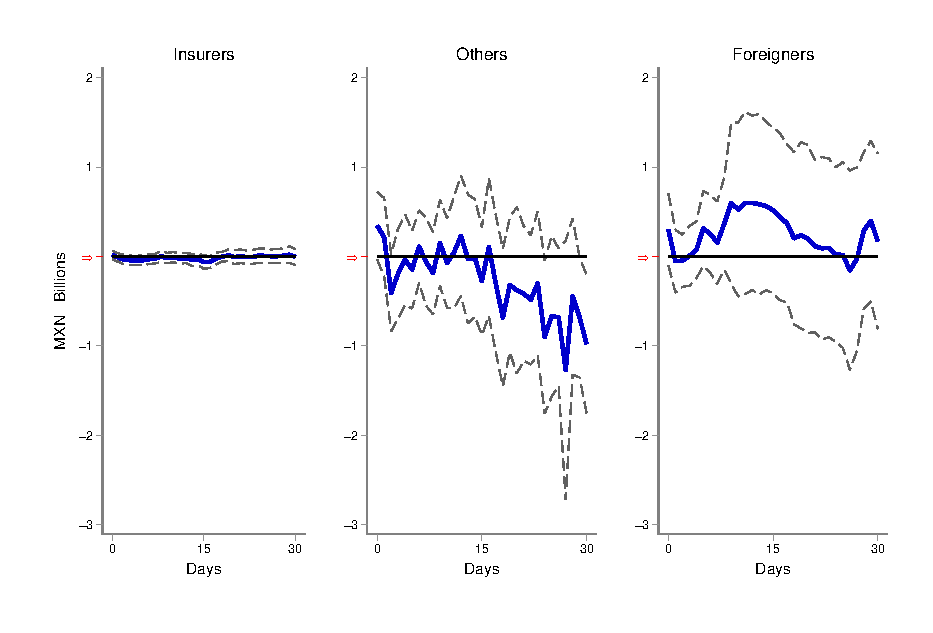
\includegraphics[trim={0.3cm 0.23cm 0.3cm 0.23cm},clip,height=0.33\textheight,width=\linewidth]{../Figures/LPs/Target/Bonds/Target11BondsInstit2.eps} \\
						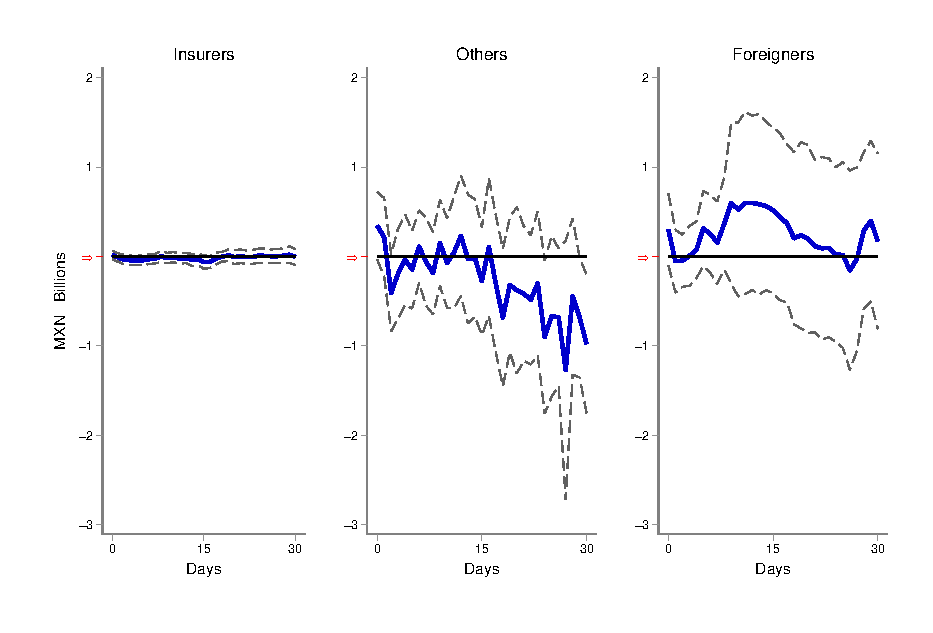
\includegraphics[trim={0.3cm 0.23cm 0.3cm 0.23cm},clip,height=0.33\textheight,width=\linewidth]{../Figures/LPs/Target/Bonds/Target11BondsInstit2.eps} \\
						\vspace{-0.35cm}
						\caption{Target  Surprise} \label{subfig:Target11BondsOther}
						\vspace{0.4cm}
					\end{subfigure}
				
					\vspace{0.1cm}
					
					\begin{subfigure}[t]{\linewidth}
%						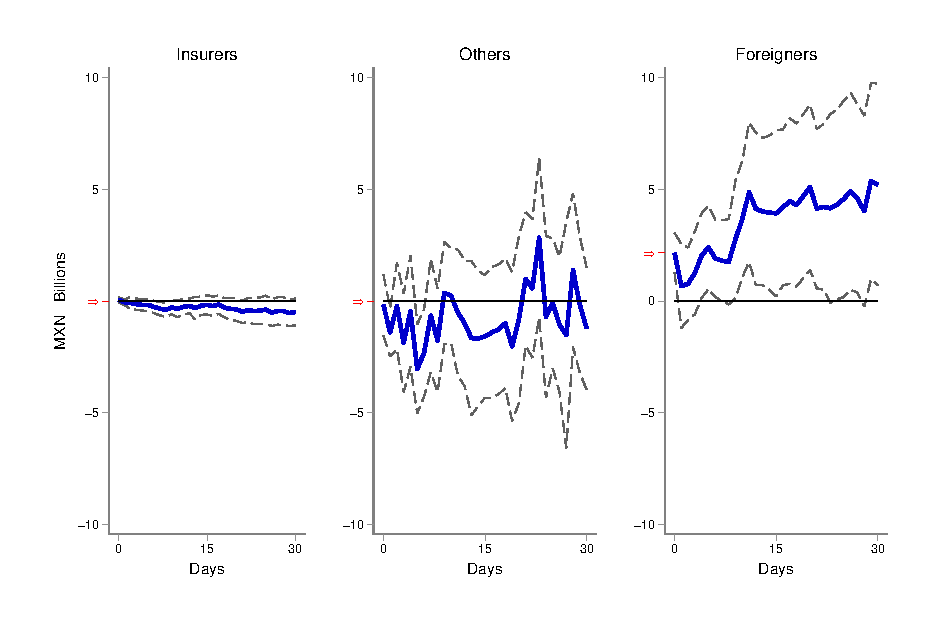
\includegraphics[trim={0.3cm 0.23cm 0.3cm 0.23cm},clip,height=0.33\textheight,width=\linewidth]{../Figures/LPs/Path/Bonds/Path11BondsInstit2.eps} \\
						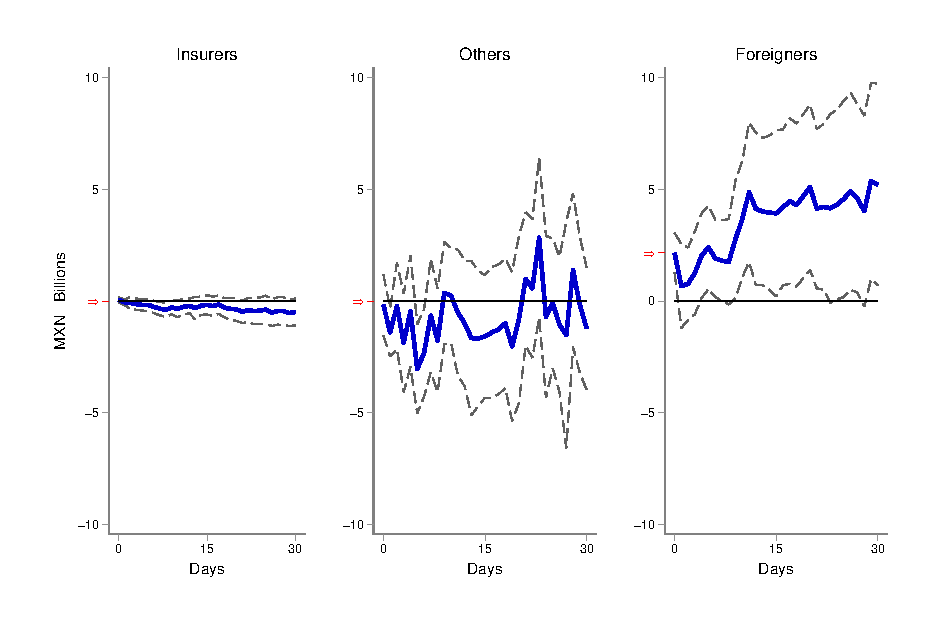
\includegraphics[trim={0.3cm 0.23cm 0.3cm 0.23cm},clip,height=0.33\textheight,width=\linewidth]{../Figures/LPs/Path/Bonds/Path11BondsInstit2.eps} \\
						\vspace{-0.35cm}
						\caption{Path Surprise} \label{subfig:Path11BondsOther}
					\end{subfigure}
					\vspace{-0.45cm}
				\end{center}
				\fignotes{This figure plots the coefficient estimates and 95\% confidence intervals for 1 basis point target and path tightening surprises for bonos flows from day \(t - 1\) to day \(t + \idxh\), where \(t\) is a day with a monetary policy announcement and \(\idxh = 0, 1, \ldots, 30\). An arrow in the vertical axis indicates the contemporaneous effect (when \(\idxh = 0\)). The surprises are equal to the target and path surprises (obtained with intraday data) on announcement days and zero otherwise. The sample includes all regular monetary policy announcements from January 2011 to \lastobsflwbdm. The 95\% confidence bands are based on robust standard errors.}
			\end{minipage}
		\end{center}
	\end{figure}
	\end{landscape}
	}
\end{document}
% trim = {<left> <lower> <right> <upper>}

Investors response is sluggish. 
This delayed adjustment in the bonos holdings of some investors aligns with the post-announcement drift displayed by the yields (see figure \ref{fig:LPYC}) and is consistent with a slow-moving capital explanation in which big players take time to respond to the surprises \parencite{BrooksKatzLustig:2019}. 
See, for instance, the responses by banks to a target surprise and by foreigners to a path surprise. 

Investors do rebalance their bonos portfolios based on their business model.
For instance, after a target tightening surprise, pension funds buy bonos but banks sell them, reflecting their different investment profiles. 
Banks have a shorter investment horizon than pension funds. 
Specifically, the average maturity of the bonos held by banks is less than 5 years, while for pension funds it is more than 10 years \parencite{Banxico:2014}. 

In particular, Mexican banks exhibit a reach-for-yield behavior. 
The response of banks to target surprises (top left panel of figure \ref{fig:LPBondsInstit}) implies that they buy bonos a few days after a target easing surprise. Intuitively, banks offset the negative effects of a target easing surprise on their current income by rebalancing their portfolio toward long-term bonds, which lowers their yields. 
Mexican banks thus respond like the yield-oriented investors described by \textcite{HansonStein:2015}, for which a monetary easing induces them to take on more interest rate risk and to push down the term premia of bond yields. 
They are therefore key for Banxico to influence the term premium. 
This result supports one of the explanations discussed in section \ref{sec:onimpactyc} of why the yield curve in Mexico responds stronger to monetary policy than the U.S. yield curve, yet it does not discard the other one. 

Finally, foreign investors are key in the transmission of path surprises. 
They reallocate their portfolios toward bonos in the month following a tightening of the monetary stance going forward. 
Their role helps to explain the strong effect of path surprises on bond yields reported in section \ref{sec:onimpactyc}. 
The response of foreign investors is thus relevant for central banks in emerging markets. 
An important implication of this result is that portfolio flows to emerging markets respond not only to the monetary policy of advanced economies \parencite{Chenetal:2014,Curcuruetal:2015,Fischer:2020}, but also to that of the host country. 

In summary, domestic and foreign investors are key in the transmission of target and path surprises.
%Chari: asset prices in emerging markets are more sensitive than capital flows to U.S. monetary policy.

}{}	% Closes \iftoggle{fulldraft}


\section{Concluding Remarks}\label{sec:conclusions}
\iftoggle{fulldraft}{					% Turn it on/off in packages.tex
	\iftoggle{toclinks}{\gototoc}{} % Turn it on/off in packages.tex, command in macros.tex
	\iftoggle{cboxes}{	   				 % Turn it on/off in packages.tex
		\begin{boxeditems}
			\item Insert: characteristics shared with AEs and unique to EMs: multidimensionality of MP is not limited to AEs vs more influence on the yield curve. 
			Insert: It is important to highlight that the multiple dimensions are not independent but complementary tools of monetary policy.
		\end{boxeditems}}{}

This paper uses a new high-frequency dataset to identify monetary policy surprises in an emerging economy. The evidence shows that the central bank conducts monetary policy by adjusting its current policy rate and by managing expectations about its future path via statements, both of which influence asset prices and portfolio flows. The multidimensionality of monetary policy is therefore not exclusive to central banks in advanced economies and does not require the zero lower bound to be binding. 

Having the ability to manage market expectations about the future path of the policy rate via statements improves the implementation of monetary policy in emerging markets. Their central banks can better influence medium- and long-term interest rates, which are relevant for the spending decisions of households and businesses. They also have more room than previously thought to deal with periods of high inflation as well as with the spillover effects of monetary policies implemented in advanced economies. 

Given the importance of statements documented here, central banks in emerging markets can follow best practices in monetary policy communications, including brief, clear and concise language without compromising the main message. References to non-monetary policy issues (e.g. structural reforms) should be minimal, if any.\footnote{On this regard, Banxico committed to issue clear and concise statements in February 2020. The guidelines are publicly available at  \url{https://www.banxico.org.mx/publicaciones-y-prensa/miscelaneos/\%7B4C09D772-2CDF-8BD6-3F04-65DE03CA6212\%7D.pdf}.}

The results in this paper can be extended in several directions. 
For instance, decomposing the Mexican sovereign yields can provide additional evidence on the transmission of the two types of monetary policy surprises. In addition, the  host country perspective for portfolio flows seems relevant for emerging markets in connection with macroprudential policies. In particular, given how foreign investors rebalance their portfolios in response to local monetary policy surprises, policymakers could be interested in the interaction of target and path surprises with different macroprudential policies, including capital controls. Finally, more research is needed to assess the extent to which the results reported here apply to other emerging markets.

}{}	% Closes \iftoggle{fulldraft}


%\section*{Acknowledgements}
%I am particularly grateful to Jonathan Wright for insightful discussions and feedback. I also thank Derin Aksit, Laurence Ball, Enrique Batiz, Christopher Carroll, Lalit Contractor, Jorge Luis García Ramírez, Karlye Dilts Stedman, Gregory Duffee, Eric Fischer, Raúl Ibarra Ramírez, Olivier Jeanne, Fabrizio López Gallo Dey, Claudia Ramírez Bulos, Alessandro Rebucci, and seminar participants at the 2020 Southern Finance Association meeting and Banco de México for their helpful comments and suggestions. The views in this paper are the sole responsibility of the author and should not be interpreted as reflecting the views of Banco de México or any other person associated with it. All remaining errors are mine.


\uspunctuation
\begin{singlespace}
	\printbibliography
\end{singlespace}

%Bennani, Hamza, 2019. "Does People's Bank of China communication matter? Evidence from stock market reaction," Emerging Markets Review, Elsevier, vol. 40(C), pages 1-1.
%Shiwei Su, Ahmad Hassan Ahmad, Justine Wood. 2019. How effective is central bank communication in emerging economies? An empirical analysis of the chinese money markets responses to the people’s bank of China’s policy communications. Review of Quantitative Finance and Accounting 52.
%Helder Ferreira de Mendonça, Joseph David Barroso Vasconcelos de Deus. 2019. Central bank forecasts and private expectations: An empirical assessment from three emerging economies. Economic Modelling.


% Figures and Tables
%\newpage
%\documentclass{article}
\usepackage{graphicx}
\usepackage[margin=1in]{geometry}
\usepackage[outdir=./]{epstopdf}  					% Avoids errors when input figures
\usepackage[labelsep=period,labelfont=bf]{caption}
%\usepackage{subcaption}

\begin{document}
	\begin{figure}[t]
		\caption{Monetary Policy Surprises in Mexico: Intraday vs. Daily Data} \label{fig:factorslines}
		\begin{center}								% center the minipage on the line
			\begin{minipage}{0.9\linewidth}
				\vspace{-0.4cm}
				\begin{center}							% center the figure inside the minipage
					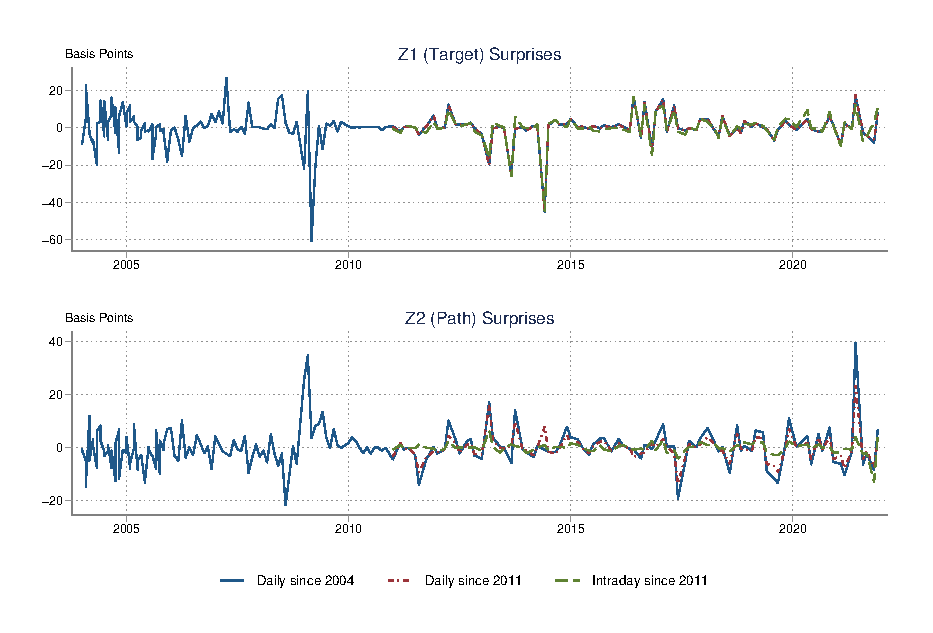
\includegraphics[width=1\textwidth,height=.4\textheight]{../Figures/factorslines.eps} \\
				\end{center}
				\vspace{-0.4cm}
				\fignotes{This figure compares the evolution of the \( \rtdone \) (target) and \( \rtdtwo \) (path) surprises obtained with daily data since 2004 (solid line) and 2011 (dash-dotted line), and with intraday data since 2011 (dashed line). The sample includes all regular monetary policy announcements up to \lastobs{}.}
			\end{minipage}
		\end{center}
	\end{figure}
\end{document}
% trim = {<left> <lower> <right> <upper>}
	% \ref{fig:factorslines}
%\documentclass{article}
\usepackage{graphicx}
\usepackage[margin=1in]{geometry}
\usepackage[outdir=./]{epstopdf}  					% Avoids errors when input figures
\usepackage[labelsep=period,labelfont=bf]{caption}
%\usepackage{afterpage}
%\usepackage{subcaption}

\begin{document}
%	\afterpage{
	\begin{figure}[t]
		\caption{Monetary Policy Dimensions} \label{fig:factorspoints}
		\begin{center}								% center the minipage on the line
			\begin{minipage}{0.9\linewidth}
				\begin{center}							% center the figure inside the minipage
%					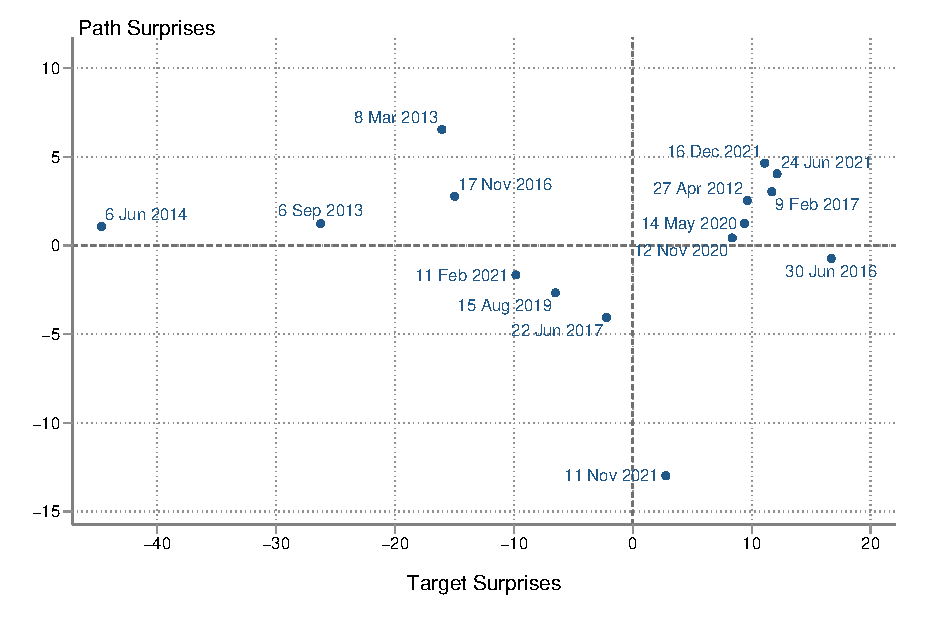
\includegraphics[width=1\textwidth,height=.4\textheight]{../Figures/factorspointstg.eps} \\
%					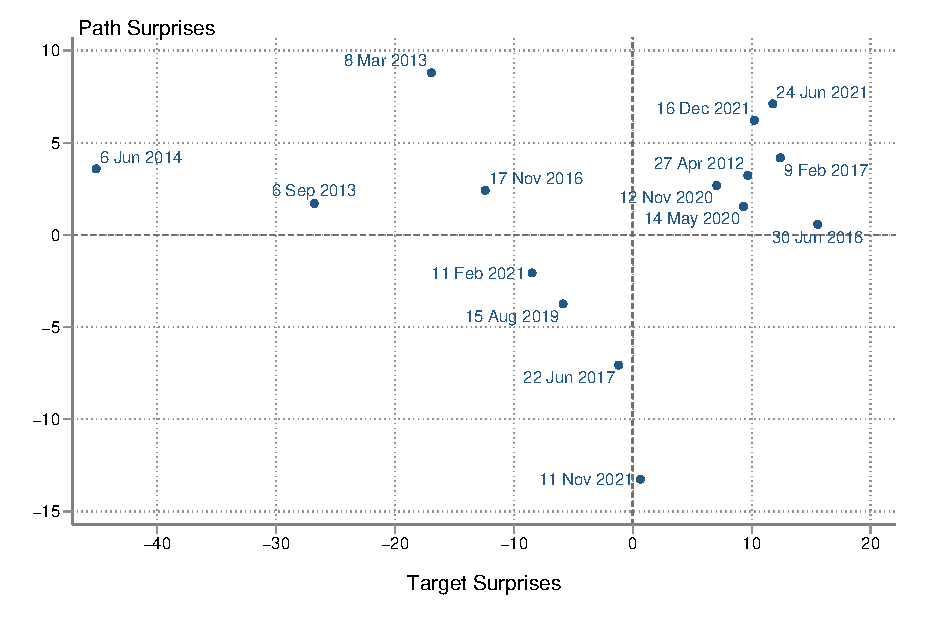
\includegraphics[width=1\textwidth,height=.4\textheight]{../Figures/factorspointswd.eps} \\
%					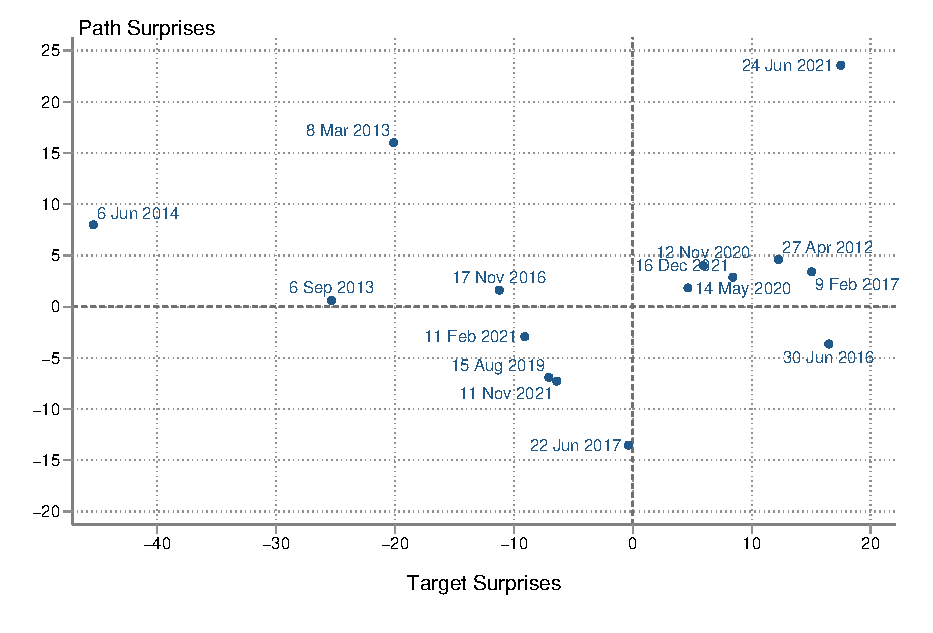
\includegraphics[width=1\textwidth,height=.4\textheight]{../Figures/factorspointsdy.eps} \\
					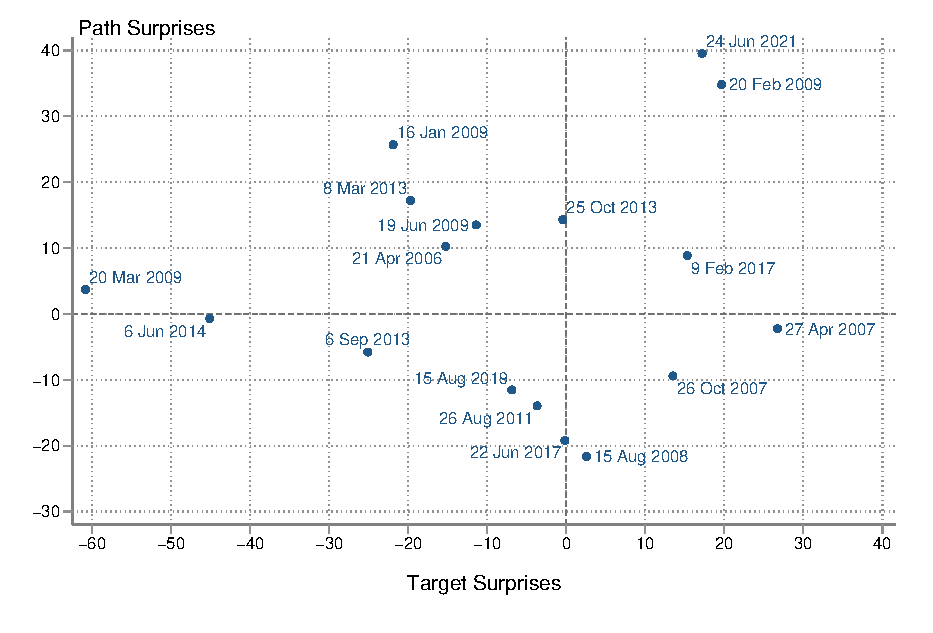
\includegraphics[width=1\textwidth,height=.4\textheight]{../Figures/factorspoints04.eps} \\
				\end{center}
				\vspace{-0.4cm}
				\fignotes{This figure plots the largest estimated target and path surprises (expressed in basis points) obtained from daily data, as explained in the main text. The sample includes all regular monetary policy announcements from January 2004 to \lastobs.} 
			\end{minipage}
		\end{center}
	\end{figure}
%	}
\end{document}
% trim = {<left> <lower> <right> <upper>}
	% \ref{fig:factorspoints}

%\begin{landscape}
%	\documentclass{article}
\usepackage[margin=1in]{geometry}
\usepackage{graphicx}
\usepackage[outdir=./]{epstopdf}  					% Avoids errors when input figures
\usepackage[labelsep=period,labelfont=bf]{caption}
\usepackage{subcaption}
\usepackage{pdflscape}
\usepackage{afterpage}
%% Personalized Macros
% Table of Contents, Tables, Subcaptions, Track Changes, Footnotes

%---------------------------------------------------------------
% Table of Contents
%---------------------------------------------------------------

% Link to ToC from section
\newcommand{\gototoc}{\vspace{-2cm} \null\hfill [\hyperlink{toc}{Go2ToC}] \newline}

% Link back to section from ToC
\newcommand{\maketoc}{
	\hypertarget{toc}{}
	\newpage
	\tableofcontents
	\vspace{2.5\bigskipamount} }

% Box with bullets for tasks to do in a section
\newenvironment{boxeditems}
	{\begin{tabular}{|p{\linewidth}|}
	\hline
	\begin{itemize}
	}
	{
	\end{itemize}
	\\ \hline
	\end{tabular} \\
	}

%---------------------------------------------------------------
% Tables
%---------------------------------------------------------------

% Estout Commands following Jörg Weber
\newcommand{\sym}[1]{\rlap{#1}}

\let\estinput=\input	% define new input command to flatten the document

\newcommand{\estauto}[2]{
	\newcolumntype{C}{>{\centering\arraybackslash}X}
	\vspace{.75ex}{
%		\begin{tabularx}{1.4\textwidth}{l*{#2}C}
		\begin{tabularx}{0.95\linewidth}{l*{#2}C}
			\toprule
			\estinput{#1}
			\\ \bottomrule
			\addlinespace[.75ex]
		\end{tabularx}
	}
}

% Allow line breaks with \\ in specialcells
\newcommand{\specialcell}[2][c]{\begin{tabular}[#1]{@{}c@{}}#2\end{tabular}}

%---------------------------------------------------------------
% Subcaptions
%---------------------------------------------------------------

% Notes after figures following Jörg Weber
\newcommand{\figtext}[1]{
	\vspace{-1ex}
	\captionsetup{justification=justified,font=footnotesize}
	\caption*{#1}
%	\captionsetup{justification=raggedright,singlelinecheck=false,font=footnotesize}
%	\caption*{\hspace{6pt}\hangindent=1.5em #1}
}

\newcommand{\fignote}[1]{\figtext{\emph{Note:~}~#1}}
\newcommand{\fignotes}[1]{\figtext{\emph{Notes:~}~#1}}

% Notes after tables
\newcommand{\tabnote}[1]{
	\begin{tablenotes}[para,flushleft]
		\footnotesize \emph{Notes:~}~#1
	\end{tablenotes}
}

%---------------------------------------------------------------
% Track Changes
%---------------------------------------------------------------

% Highlight changes in revised version with color
\newcommand{\textchange}[1]{\iftoggle{revised}{\textcolor{blue}{#1}}{#1}}

%---------------------------------------------------------------
% Footnotes
%---------------------------------------------------------------

%% Change the look of foonote indicators
%\makeatletter
%\let \@makefntextorig \@makefntext
%\newcommand{\@makefntextcustom}[1]{%
%	\thefootnote.\enskip #1%
%}
%\renewcommand{\@makefntext}[1]{\@makefntextcustom{#1}}
%\makeatother
%
%% Change the look of endnote indicators
%\renewcommand{\makeenmark}{\hbox{$^{\theenmark}$}}
%\makeatletter
%\def\enoteformat{%
%	\rightskip\z@ \leftskip\z@ \parindent=1.8em
%	\leavevmode{\setbox\z@=\lastbox}\llap{\theenmark.\enskip}%
%}
%\makeatother			   % Personalized commands
%% Personalized Macros
% Variable Definitions, Equations

%---------------------------------------------------------------
% Variable Definitions
%---------------------------------------------------------------
\providecommand{\tiie}{TIIE28D}
\providecommand{\lastobs}{December 2021}
\providecommand{\lastobsfx}{November 2021}
\providecommand{\lastobsflwbdm}{December 2021}
\providecommand{\lastobsflwtic}{August 2021}
\providecommand{\idxt}{t}
\providecommand{\idxh}{h}
\providecommand{\idxi}{i}
\providecommand{\idxsfwd}{\idxt+\idxh}
\providecommand{\idxslag}{\idxt-1}
\providecommand{\yld}{y}
\providecommand{\ctrls}{z}
\providecommand{\hld}{H}
\providecommand{\depvar}{\Delta \yld_{\idxt}}
\providecommand{\mps}{\Delta x_{\idxt}}
\providecommand{\depvarclean}{\depvar^{*}}
\providecommand{\mpsclean}{\mps^{*}}
\providecommand{\paramB}{\beta}
\providecommand{\intrcpt}{\paramB_{0}}
\providecommand{\slopetrgt}{\paramB_{1}}
\providecommand{\slopepath}{\paramB_{2}}
\providecommand{\assets}{X}
\providecommand{\factors}{F}
\providecommand{\loadings}{\Lambda}
\providecommand{\rotated}{Z}
\providecommand{\rmatrix}{U}
\providecommand{\rtdone}{\rotated_{1}}
\providecommand{\rtdtwo}{\rotated_{2}}
\providecommand{\rtdonereg}{Target_{\idxt}}
\providecommand{\rtdtworeg}{Path_{\idxt}}
\providecommand{\lagidx}{j}
\providecommand{\lagorder}{p}
\providecommand{\lagparam}{\gamma}   %\alpha
\providecommand{\lagoper}{L}
\providecommand{\depvarflw}{\Delta \hld_{\idxt}}
\providecommand{\flows}{w_{\idxt}}
\providecommand{\flowslag}{w_{\idxt - \lagidx}}
\providecommand{\lagsum}{\sum_{\lagidx = 1}^{\lagorder} \lagparam_{\lagidx} \flowslag}
\providecommand{\lagsumh}{\sum_{\lagidx = 1}^{\lagorder} \lagparam^{\lagidx}_\idxh \flowslag}
\providecommand{\dimobs}{T}
\providecommand{\dimassets}{n}
\providecommand{\dimfactors}{k}
\providecommand{\dimnull}{\dimfactors_{0}}
\providecommand{\dimsassets}{\dimobs \times \dimassets}
\providecommand{\dimsfactors}{\dimobs \times \dimfactors}
\providecommand{\dimsloadings}{\dimfactors \times \dimassets}
\providecommand{\errorreg}{\varepsilon_{\idxt}}
\providecommand{\errorfac}{\zeta}
\providecommand{\errorflows}{\nu_{\idxt}}
\providecommand{\Rsqrt}{R^{2}}

\providecommand{\dpv}{y}
\providecommand{\idv}{x}
\providecommand{\omv}{\omega}
\providecommand{\dpvstar}{\dpv^{*}}
\providecommand{\idvstar}{\idv^{*}}
\providecommand{\jobs}{Jobs}
\providecommand{\errortrue}{\varepsilon}
\providecommand{\errormix}{\tau}
\providecommand{\melhs}{\nu}
\providecommand{\merhs}{u}
\providecommand{\mean}{\mu}
\providecommand{\covar}{\sigma}
\providecommand{\corr}{\rho}
\providecommand{\var}{\covar^{2}}
\providecommand{\meanE}{\mean_{\errortrue}}
\providecommand{\meanU}{\mean_{\merhs}}
\providecommand{\meanV}{\mean_{\melhs}}
\providecommand{\varE}{\var_{\errortrue}}
\providecommand{\varU}{\var_{\merhs}}
\providecommand{\varV}{\var_{\melhs}}
\providecommand{\varX}{\var_{\idv}}
\providecommand{\varXstar}{\var_{\idvstar}}
\providecommand{\covarEX}{\covar_{\errortrue \idvstar}}
\providecommand{\covarUE}{\covar_{\merhs \errortrue}}
\providecommand{\covarVE}{\covar_{\melhs \errortrue}}
\providecommand{\covarUX}{\covar_{\merhs \idvstar}}
\providecommand{\covarUY}{\covar_{\merhs \dpvstar}}
\providecommand{\covarVX}{\covar_{\melhs \idvstar}}
\providecommand{\covarVY}{\covar_{\melhs \dpvstar}}
\providecommand{\covarUV}{\covar_{\merhs \melhs}}
\providecommand{\covarWXe}{\covar_{\omv \idv}}
\providecommand{\covarVXe}{\covar_{\melhs \idv}}
\providecommand{\corrUV}{\corr_{\merhs \melhs}}
\providecommand{\corrUX}{\corr_{\merhs \idvstar}}
\providecommand{\corrUY}{\corr_{\merhs \dpvstar}}
\providecommand{\corrVX}{\corr_{\melhs \idvstar}}
\providecommand{\corrVY}{\corr_{\melhs \dpvstar}}
\providecommand{\paramG}{\gamma}
\providecommand{\estimB}{\hat{\paramB}}
\providecommand{\paramSE}{\varE}
\providecommand{\estimSE}{\hat{\paramSE}}
\providecommand{\paramAVB}{s}
\providecommand{\estimAVB}{\hat{\paramAVB}}
\providecommand{\attnfactor}{\lambda}
\providecommand{\plim}{\mathrm{plim}}

\providecommand{\reg}{\delta}
\providecommand{\regVonX}{\reg_{\melhs \idv}}
\providecommand{\regWonX}{\reg_{\omv \idv}}
\providecommand{\regWonXstar}{\reg_{\omv \idvstar}}

%---------------------------------------------------------------
% Equations
%---------------------------------------------------------------
\newcommand{\eqOneFac}{\depvar = \intrcpt + \slopetrgt \mps + \errorreg}
\newcommand{\eqOneFacOV}{\depvar = \intrcpt + \slopetrgt PRS_{\idxt} + \paramB_{2} \Delta VIX_{\idxt} + \paramB_{3} \Delta USY_{\idxt} + \paramB_{4} WTI_{\idxt} + \paramB_{5} \jobs_{\idxt} + \errorreg}
\newcommand{\eqTwoFacP}{\depvar = \intrcpt + \slopetrgt \rtdonereg + \slopepath \rtdtworeg + \errorreg}
\newcommand{\eqTwoFacF}{\depvarflw = \intrcpt + \slopetrgt \rtdonereg + \slopepath \rtdtworeg + \errorreg}
\newcommand{\eqPCA}{\assets = \factors \loadings + \errorfac}
\newcommand{\eqRotation}{\rotated = \factors \, \rmatrix}
\newcommand{\eqFlows}{\flows = \intrcpt + \slopetrgt \rtdonereg + \slopepath \rtdtworeg + \lagsum + \eta^{'} \ctrls_{\idxslag} + \errorflows}
%\newcommand{\eqLagPoly}{\lagsum = 1 - \lagparam_{1} \lagoper - \lagparam_{2} \lagoper^{2} - \ldots - \lagparam_{\lagorder} \lagoper^{\lagorder}}
\newcommand{\eqAsym}{\yld_{\idxt} = \intrcpt + \paramB_{1} \rtdonereg \mathds{1} \left(\rtdonereg > 0 \right) + \paramB_{2} \rtdonereg \mathds{1} \left(\rtdonereg < 0 \right) \\ + \paramB_{3} \rtdtworeg \mathds{1} \left(\rtdtworeg > 0 \right) + \paramB_{4} \rtdtworeg \mathds{1} \left(\rtdtworeg < 0 \right) + \errorreg}

\newcommand{\eqDGP}{\dpvstar &= \paramB \idvstar + \errortrue}
\newcommand{\eqDGPme}{\dpv = \paramB \idv + \errormix = \paramB \idv + \eqErrormix}
\newcommand{\eqDGPov}{\dpvstar = \paramB \idvstar + \paramG \omv +  \errortrue}
\newcommand{\eqMEdpv}{\dpv &= \dpvstar + \melhs}
\newcommand{\eqMEidv}{\idv &= \idvstar + \merhs}
\newcommand{\eqAtten}{\attnfactor = \frac{\varXstar}{\varXstar + \varU}}
\newcommand{\eqAttenInLine}{\attnfactor = \varXstar / \left(\varXstar + \varU\right) }
\newcommand{\eqErrormix}{\errortrue - \paramB \merhs + \melhs}

\newcommand{\eqPlimBstd}{\plim \left( \estimB \right) = \frac{cov(\idv, \dpvstar)}{var(\idv)} = \frac{cov(\idvstar + \merhs, \paramB \idvstar + \errortrue)}{var(\idvstar + \merhs)} = \paramB \frac{\varXstar}{\varXstar + \varU} = \paramB \attnfactor}
\newcommand{\eqPlimBstdshort}{\plim (\estimB) = \paramB \attnfactor}

%\newcommand{\eqPlimSstd}{\plim \left( \estimAVB \right) = \plim \left( \frac{\estimSE}{\hat{\varX}} \right) = \frac{\varE + (1-\attnfactor)^{2} \paramB^{2} \varXstar + \attnfactor^{2} \paramB^{2} \varU}{\varXstar + \varU} = \attnfactor \paramAVB + \attnfactor(1 - \attnfactor) \paramB^{2}}
\newcommand{\eqPlimSstd}{\plim \left( \estimAVB \right) = \attnfactor \paramAVB + \attnfactor(1 - \attnfactor) \paramB^{2}}

\newcommand{\eqPlimBnew}{\plim \left( \estimB \right) 
	= \frac{cov(\idv, \dpv)}{var(\idv)} 
	= \frac{cov(\idvstar + \merhs, \paramB \idvstar + \paramG \omv + \errortrue)}{var(\idvstar + \merhs)} 
	= \frac{\paramB \varXstar + \paramG \covarWXe}{\varXstar + \varU}  }

\newcommand{\eqPlimBbias}{\plim \left( \estimB \right)
	= \paramB \frac{\varXstar}{\varX} + \paramG \frac{\covarWXe}{\varX}
	= \paramB \attnfactor + \paramG \regWonX}

\providecommand{\errordepvar}{e_{y}}
\providecommand{\errormps}{e_{x}}
\newcommand{\eqMEdepvar}{\depvar &= \depvarclean + \errordepvar}
\newcommand{\eqMEmps}{\mps &= \mpsclean + \errormps}

\newcommand{\eqLPrhs}{\alpha_{\idxh} + \beta^{1}_{\idxh} \; \rtdonereg +  \beta^{2}_{\idxh} \; \rtdtworeg + \eta^{'}_{\idxh} \ctrls_{\idxslag}  + u_{\idxsfwd}}

\newcommand{\eqLPprices}{\yld_{\idxsfwd} - \yld_{\idxslag} = \eqLPrhs} 

\newcommand{\eqLPflows}{\hld_{\idxsfwd} - \hld_{\idxslag} = \eqLPrhs} 
% \gamma_{\idxh} \Delta \yld_{\idxslag} 
%\alpha_{\idxh} + \beta^{1}_{\idxh} \; \rtdonereg +  \beta^{2}_{\idxh} \; \rtdtworeg + \lagsumh + \eta_{\idxh} \ctrls_{\idxslag}  + u_{\idxsfwd}

\newcommand{\eqLP}{\yld_{\idxsfwd} - \yld_{\idxslag} = \alpha_{\idxh} + \gamma_{\idxh} \mps + u_{\idxsfwd}} 			    % Personalized commands
%\pagestyle{empty}

\begin{document}
	\afterpage{
	\begin{landscape}
	\begin{figure}[tbph]
		\caption{Response of the Yield Curve to Target and Path Surprises} \label{fig:LPYC}
		\begin{center}
			\begin{minipage}{\linewidth}
				\begin{center}
					\begin{subfigure}[t]{\linewidth}
						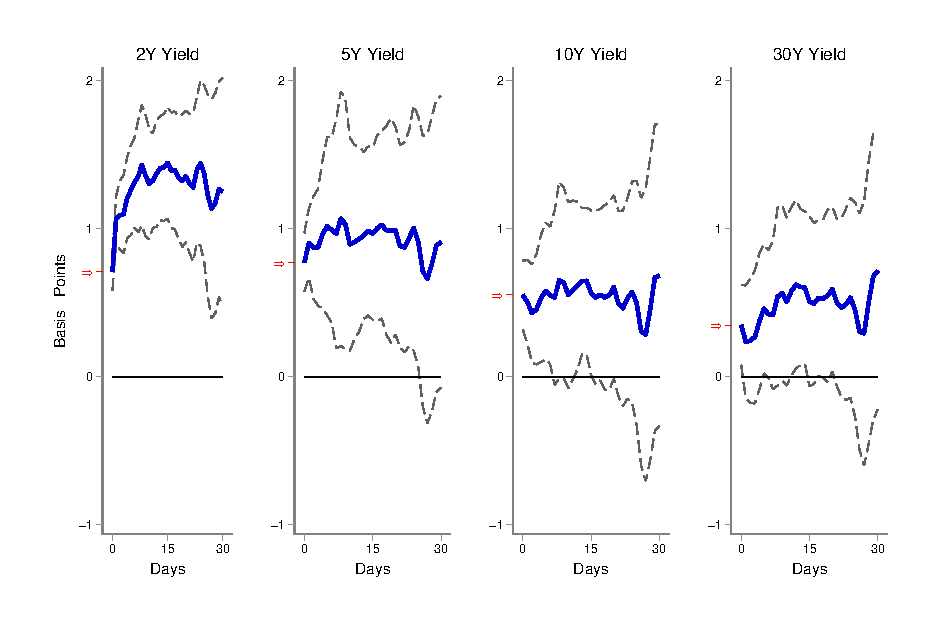
\includegraphics[trim={0.3cm 0.23cm 0.3cm 0.23cm},clip,height=0.33\textheight,width=\linewidth]{../Figures/LPs/Target/Target11YC.eps} \\
%						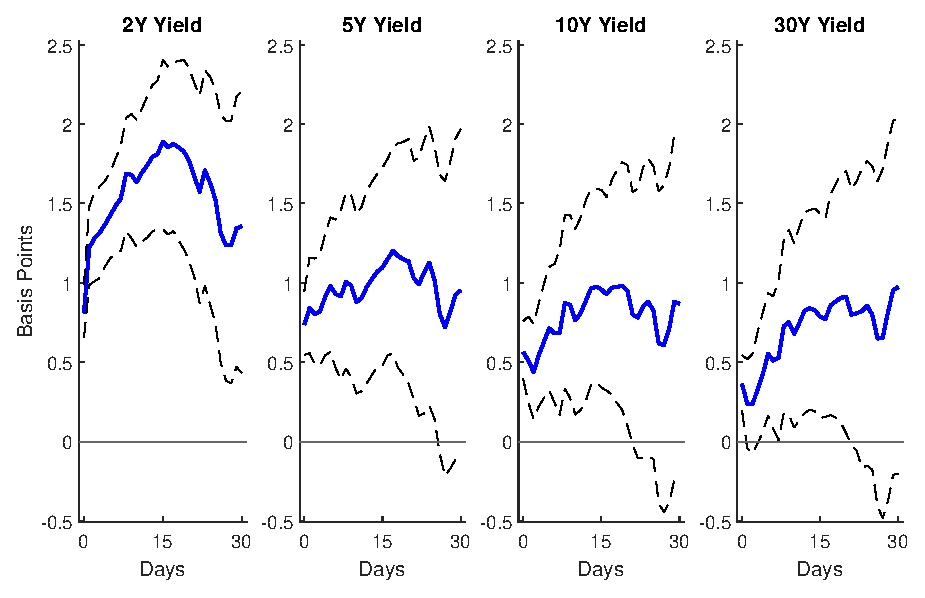
\includegraphics[trim={0.3cm 0.23cm 0.3cm 0.23cm},clip,height=0.33\textheight,width=\linewidth]{../Target/Target11YC} \\
						\vspace{-0.35cm}
						\caption{Target Surprises} \label{subfig:Target11YC}
						\vspace{0.4cm}
					\end{subfigure}
				
					\vspace{0.1cm}
					
					\begin{subfigure}[t]{\linewidth}
						\includegraphics[trim={0.3cm 0.23cm 0.3cm 0.23cm},clip,height=0.33\textheight,width=\linewidth]{../Figures/LPs/Path/Path11YC.eps} \\
%						\includegraphics[trim={0.3cm 0.23cm 0.3cm 0.23cm},clip,height=0.33\textheight,width=\linewidth]{../Path/Path11YC} \\
						\vspace{-0.35cm}
						\caption{Path Surprises} \label{subfig:Path11YC}
					\end{subfigure}
					\vspace{-0.45cm}
				\end{center}
				\fignotes{This figure plots the coefficient estimates and 95\% confidence intervals for 1 basis point target and path tightening surprises for yield changes from close of day \(t - 1\) to day \(t + \idxh\), where \(t\) is a day with a monetary policy announcement and \(\idxh = 0, 1, \ldots, 30\). An arrow in the vertical axis indicates the contemporaneous effect (when \(\idxh = 0\)). The surprises are equal to the target and path surprises (obtained with intraday data) on announcement days and zero otherwise. The sample includes all regular monetary policy announcements from January 2011 to \lastobs. The 95\% confidence bands are based on robust standard errors.}
			\end{minipage}
		\end{center}
	\end{figure}
	\end{landscape}
	}
\end{document}
% trim = {<left> <lower> <right> <upper>}
%\end{landscape}
%\pagebreak[4]

%\documentclass{article}
\usepackage{graphicx}
\usepackage[margin=1in]{geometry}
\usepackage[outdir=./]{epstopdf}  					% Avoids errors when input figures
\usepackage[labelsep=period,labelfont=bf]{caption}
%\usepackage{subcaption}
%% Personalized Macros
% Table of Contents, Tables, Subcaptions, Track Changes, Footnotes

%---------------------------------------------------------------
% Table of Contents
%---------------------------------------------------------------

% Link to ToC from section
\newcommand{\gototoc}{\vspace{-2cm} \null\hfill [\hyperlink{toc}{Go2ToC}] \newline}

% Link back to section from ToC
\newcommand{\maketoc}{
	\hypertarget{toc}{}
	\newpage
	\tableofcontents
	\vspace{2.5\bigskipamount} }

% Box with bullets for tasks to do in a section
\newenvironment{boxeditems}
	{\begin{tabular}{|p{\linewidth}|}
	\hline
	\begin{itemize}
	}
	{
	\end{itemize}
	\\ \hline
	\end{tabular} \\
	}

%---------------------------------------------------------------
% Tables
%---------------------------------------------------------------

% Estout Commands following Jörg Weber
\newcommand{\sym}[1]{\rlap{#1}}

\let\estinput=\input	% define new input command to flatten the document

\newcommand{\estauto}[2]{
	\newcolumntype{C}{>{\centering\arraybackslash}X}
	\vspace{.75ex}{
%		\begin{tabularx}{1.4\textwidth}{l*{#2}C}
		\begin{tabularx}{0.95\linewidth}{l*{#2}C}
			\toprule
			\estinput{#1}
			\\ \bottomrule
			\addlinespace[.75ex]
		\end{tabularx}
	}
}

% Allow line breaks with \\ in specialcells
\newcommand{\specialcell}[2][c]{\begin{tabular}[#1]{@{}c@{}}#2\end{tabular}}

%---------------------------------------------------------------
% Subcaptions
%---------------------------------------------------------------

% Notes after figures following Jörg Weber
\newcommand{\figtext}[1]{
	\vspace{-1ex}
	\captionsetup{justification=justified,font=footnotesize}
	\caption*{#1}
%	\captionsetup{justification=raggedright,singlelinecheck=false,font=footnotesize}
%	\caption*{\hspace{6pt}\hangindent=1.5em #1}
}

\newcommand{\fignote}[1]{\figtext{\emph{Note:~}~#1}}
\newcommand{\fignotes}[1]{\figtext{\emph{Notes:~}~#1}}

% Notes after tables
\newcommand{\tabnote}[1]{
	\begin{tablenotes}[para,flushleft]
		\footnotesize \emph{Notes:~}~#1
	\end{tablenotes}
}

%---------------------------------------------------------------
% Track Changes
%---------------------------------------------------------------

% Highlight changes in revised version with color
\newcommand{\textchange}[1]{\iftoggle{revised}{\textcolor{blue}{#1}}{#1}}

%---------------------------------------------------------------
% Footnotes
%---------------------------------------------------------------

%% Change the look of foonote indicators
%\makeatletter
%\let \@makefntextorig \@makefntext
%\newcommand{\@makefntextcustom}[1]{%
%	\thefootnote.\enskip #1%
%}
%\renewcommand{\@makefntext}[1]{\@makefntextcustom{#1}}
%\makeatother
%
%% Change the look of endnote indicators
%\renewcommand{\makeenmark}{\hbox{$^{\theenmark}$}}
%\makeatletter
%\def\enoteformat{%
%	\rightskip\z@ \leftskip\z@ \parindent=1.8em
%	\leavevmode{\setbox\z@=\lastbox}\llap{\theenmark.\enskip}%
%}
%\makeatother			% Personalized commands
%% Personalized Macros
% Variable Definitions, Equations

%---------------------------------------------------------------
% Variable Definitions
%---------------------------------------------------------------
\providecommand{\tiie}{TIIE28D}
\providecommand{\lastobs}{December 2021}
\providecommand{\lastobsfx}{November 2021}
\providecommand{\lastobsflwbdm}{December 2021}
\providecommand{\lastobsflwtic}{August 2021}
\providecommand{\idxt}{t}
\providecommand{\idxh}{h}
\providecommand{\idxi}{i}
\providecommand{\idxsfwd}{\idxt+\idxh}
\providecommand{\idxslag}{\idxt-1}
\providecommand{\yld}{y}
\providecommand{\ctrls}{z}
\providecommand{\hld}{H}
\providecommand{\depvar}{\Delta \yld_{\idxt}}
\providecommand{\mps}{\Delta x_{\idxt}}
\providecommand{\depvarclean}{\depvar^{*}}
\providecommand{\mpsclean}{\mps^{*}}
\providecommand{\paramB}{\beta}
\providecommand{\intrcpt}{\paramB_{0}}
\providecommand{\slopetrgt}{\paramB_{1}}
\providecommand{\slopepath}{\paramB_{2}}
\providecommand{\assets}{X}
\providecommand{\factors}{F}
\providecommand{\loadings}{\Lambda}
\providecommand{\rotated}{Z}
\providecommand{\rmatrix}{U}
\providecommand{\rtdone}{\rotated_{1}}
\providecommand{\rtdtwo}{\rotated_{2}}
\providecommand{\rtdonereg}{Target_{\idxt}}
\providecommand{\rtdtworeg}{Path_{\idxt}}
\providecommand{\lagidx}{j}
\providecommand{\lagorder}{p}
\providecommand{\lagparam}{\gamma}   %\alpha
\providecommand{\lagoper}{L}
\providecommand{\depvarflw}{\Delta \hld_{\idxt}}
\providecommand{\flows}{w_{\idxt}}
\providecommand{\flowslag}{w_{\idxt - \lagidx}}
\providecommand{\lagsum}{\sum_{\lagidx = 1}^{\lagorder} \lagparam_{\lagidx} \flowslag}
\providecommand{\lagsumh}{\sum_{\lagidx = 1}^{\lagorder} \lagparam^{\lagidx}_\idxh \flowslag}
\providecommand{\dimobs}{T}
\providecommand{\dimassets}{n}
\providecommand{\dimfactors}{k}
\providecommand{\dimnull}{\dimfactors_{0}}
\providecommand{\dimsassets}{\dimobs \times \dimassets}
\providecommand{\dimsfactors}{\dimobs \times \dimfactors}
\providecommand{\dimsloadings}{\dimfactors \times \dimassets}
\providecommand{\errorreg}{\varepsilon_{\idxt}}
\providecommand{\errorfac}{\zeta}
\providecommand{\errorflows}{\nu_{\idxt}}
\providecommand{\Rsqrt}{R^{2}}

\providecommand{\dpv}{y}
\providecommand{\idv}{x}
\providecommand{\omv}{\omega}
\providecommand{\dpvstar}{\dpv^{*}}
\providecommand{\idvstar}{\idv^{*}}
\providecommand{\jobs}{Jobs}
\providecommand{\errortrue}{\varepsilon}
\providecommand{\errormix}{\tau}
\providecommand{\melhs}{\nu}
\providecommand{\merhs}{u}
\providecommand{\mean}{\mu}
\providecommand{\covar}{\sigma}
\providecommand{\corr}{\rho}
\providecommand{\var}{\covar^{2}}
\providecommand{\meanE}{\mean_{\errortrue}}
\providecommand{\meanU}{\mean_{\merhs}}
\providecommand{\meanV}{\mean_{\melhs}}
\providecommand{\varE}{\var_{\errortrue}}
\providecommand{\varU}{\var_{\merhs}}
\providecommand{\varV}{\var_{\melhs}}
\providecommand{\varX}{\var_{\idv}}
\providecommand{\varXstar}{\var_{\idvstar}}
\providecommand{\covarEX}{\covar_{\errortrue \idvstar}}
\providecommand{\covarUE}{\covar_{\merhs \errortrue}}
\providecommand{\covarVE}{\covar_{\melhs \errortrue}}
\providecommand{\covarUX}{\covar_{\merhs \idvstar}}
\providecommand{\covarUY}{\covar_{\merhs \dpvstar}}
\providecommand{\covarVX}{\covar_{\melhs \idvstar}}
\providecommand{\covarVY}{\covar_{\melhs \dpvstar}}
\providecommand{\covarUV}{\covar_{\merhs \melhs}}
\providecommand{\covarWXe}{\covar_{\omv \idv}}
\providecommand{\covarVXe}{\covar_{\melhs \idv}}
\providecommand{\corrUV}{\corr_{\merhs \melhs}}
\providecommand{\corrUX}{\corr_{\merhs \idvstar}}
\providecommand{\corrUY}{\corr_{\merhs \dpvstar}}
\providecommand{\corrVX}{\corr_{\melhs \idvstar}}
\providecommand{\corrVY}{\corr_{\melhs \dpvstar}}
\providecommand{\paramG}{\gamma}
\providecommand{\estimB}{\hat{\paramB}}
\providecommand{\paramSE}{\varE}
\providecommand{\estimSE}{\hat{\paramSE}}
\providecommand{\paramAVB}{s}
\providecommand{\estimAVB}{\hat{\paramAVB}}
\providecommand{\attnfactor}{\lambda}
\providecommand{\plim}{\mathrm{plim}}

\providecommand{\reg}{\delta}
\providecommand{\regVonX}{\reg_{\melhs \idv}}
\providecommand{\regWonX}{\reg_{\omv \idv}}
\providecommand{\regWonXstar}{\reg_{\omv \idvstar}}

%---------------------------------------------------------------
% Equations
%---------------------------------------------------------------
\newcommand{\eqOneFac}{\depvar = \intrcpt + \slopetrgt \mps + \errorreg}
\newcommand{\eqOneFacOV}{\depvar = \intrcpt + \slopetrgt PRS_{\idxt} + \paramB_{2} \Delta VIX_{\idxt} + \paramB_{3} \Delta USY_{\idxt} + \paramB_{4} WTI_{\idxt} + \paramB_{5} \jobs_{\idxt} + \errorreg}
\newcommand{\eqTwoFacP}{\depvar = \intrcpt + \slopetrgt \rtdonereg + \slopepath \rtdtworeg + \errorreg}
\newcommand{\eqTwoFacF}{\depvarflw = \intrcpt + \slopetrgt \rtdonereg + \slopepath \rtdtworeg + \errorreg}
\newcommand{\eqPCA}{\assets = \factors \loadings + \errorfac}
\newcommand{\eqRotation}{\rotated = \factors \, \rmatrix}
\newcommand{\eqFlows}{\flows = \intrcpt + \slopetrgt \rtdonereg + \slopepath \rtdtworeg + \lagsum + \eta^{'} \ctrls_{\idxslag} + \errorflows}
%\newcommand{\eqLagPoly}{\lagsum = 1 - \lagparam_{1} \lagoper - \lagparam_{2} \lagoper^{2} - \ldots - \lagparam_{\lagorder} \lagoper^{\lagorder}}
\newcommand{\eqAsym}{\yld_{\idxt} = \intrcpt + \paramB_{1} \rtdonereg \mathds{1} \left(\rtdonereg > 0 \right) + \paramB_{2} \rtdonereg \mathds{1} \left(\rtdonereg < 0 \right) \\ + \paramB_{3} \rtdtworeg \mathds{1} \left(\rtdtworeg > 0 \right) + \paramB_{4} \rtdtworeg \mathds{1} \left(\rtdtworeg < 0 \right) + \errorreg}

\newcommand{\eqDGP}{\dpvstar &= \paramB \idvstar + \errortrue}
\newcommand{\eqDGPme}{\dpv = \paramB \idv + \errormix = \paramB \idv + \eqErrormix}
\newcommand{\eqDGPov}{\dpvstar = \paramB \idvstar + \paramG \omv +  \errortrue}
\newcommand{\eqMEdpv}{\dpv &= \dpvstar + \melhs}
\newcommand{\eqMEidv}{\idv &= \idvstar + \merhs}
\newcommand{\eqAtten}{\attnfactor = \frac{\varXstar}{\varXstar + \varU}}
\newcommand{\eqAttenInLine}{\attnfactor = \varXstar / \left(\varXstar + \varU\right) }
\newcommand{\eqErrormix}{\errortrue - \paramB \merhs + \melhs}

\newcommand{\eqPlimBstd}{\plim \left( \estimB \right) = \frac{cov(\idv, \dpvstar)}{var(\idv)} = \frac{cov(\idvstar + \merhs, \paramB \idvstar + \errortrue)}{var(\idvstar + \merhs)} = \paramB \frac{\varXstar}{\varXstar + \varU} = \paramB \attnfactor}
\newcommand{\eqPlimBstdshort}{\plim (\estimB) = \paramB \attnfactor}

%\newcommand{\eqPlimSstd}{\plim \left( \estimAVB \right) = \plim \left( \frac{\estimSE}{\hat{\varX}} \right) = \frac{\varE + (1-\attnfactor)^{2} \paramB^{2} \varXstar + \attnfactor^{2} \paramB^{2} \varU}{\varXstar + \varU} = \attnfactor \paramAVB + \attnfactor(1 - \attnfactor) \paramB^{2}}
\newcommand{\eqPlimSstd}{\plim \left( \estimAVB \right) = \attnfactor \paramAVB + \attnfactor(1 - \attnfactor) \paramB^{2}}

\newcommand{\eqPlimBnew}{\plim \left( \estimB \right) 
	= \frac{cov(\idv, \dpv)}{var(\idv)} 
	= \frac{cov(\idvstar + \merhs, \paramB \idvstar + \paramG \omv + \errortrue)}{var(\idvstar + \merhs)} 
	= \frac{\paramB \varXstar + \paramG \covarWXe}{\varXstar + \varU}  }

\newcommand{\eqPlimBbias}{\plim \left( \estimB \right)
	= \paramB \frac{\varXstar}{\varX} + \paramG \frac{\covarWXe}{\varX}
	= \paramB \attnfactor + \paramG \regWonX}

\providecommand{\errordepvar}{e_{y}}
\providecommand{\errormps}{e_{x}}
\newcommand{\eqMEdepvar}{\depvar &= \depvarclean + \errordepvar}
\newcommand{\eqMEmps}{\mps &= \mpsclean + \errormps}

\newcommand{\eqLPrhs}{\alpha_{\idxh} + \beta^{1}_{\idxh} \; \rtdonereg +  \beta^{2}_{\idxh} \; \rtdtworeg + \eta^{'}_{\idxh} \ctrls_{\idxslag}  + u_{\idxsfwd}}

\newcommand{\eqLPprices}{\yld_{\idxsfwd} - \yld_{\idxslag} = \eqLPrhs} 

\newcommand{\eqLPflows}{\hld_{\idxsfwd} - \hld_{\idxslag} = \eqLPrhs} 
% \gamma_{\idxh} \Delta \yld_{\idxslag} 
%\alpha_{\idxh} + \beta^{1}_{\idxh} \; \rtdonereg +  \beta^{2}_{\idxh} \; \rtdtworeg + \lagsumh + \eta_{\idxh} \ctrls_{\idxslag}  + u_{\idxsfwd}

\newcommand{\eqLP}{\yld_{\idxsfwd} - \yld_{\idxslag} = \alpha_{\idxh} + \gamma_{\idxh} \mps + u_{\idxsfwd}} 			    % Personalized commands

\begin{document}
	\begin{figure}[!htb]
		\caption{Holdings of Cetes and Bonos by Nationality} \label{fig:frgnvsdmstc}
		\begin{center}								% center the minipage on the line
			\begin{minipage}{0.9\linewidth}
%				\vspace{-0.4cm}
				\begin{center}							% center the figure inside the minipage
					\includegraphics[width=1\textwidth,height=.3\textheight]{../Figures/Flows/frgnvsdmstc} \\
%					\includegraphics[width=1\textwidth,height=.3\textheight]{frgnvsdmstc} \\
				\end{center}
%				\vspace{-0.4cm}
				\fignotes{This figure shows the net holdings of Mexican Treasury bills (cetes) and fixed-rate sovereign bonds (bonos) by investor nationality from January 2011 to \lastobsflwbdm.}
			\end{minipage}
		\end{center}
	\end{figure}
\end{document}
% trim = {<left> <lower> <right> <upper>}
%\documentclass{article}
\usepackage{graphicx}
\usepackage[margin=1in]{geometry}
\usepackage[outdir=./]{epstopdf}  					% Avoids errors when input figures
\usepackage[labelsep=period,labelfont=bf]{caption}
%\usepackage{subcaption}
%% Personalized Macros
% Table of Contents, Tables, Subcaptions, Track Changes, Footnotes

%---------------------------------------------------------------
% Table of Contents
%---------------------------------------------------------------

% Link to ToC from section
\newcommand{\gototoc}{\vspace{-2cm} \null\hfill [\hyperlink{toc}{Go2ToC}] \newline}

% Link back to section from ToC
\newcommand{\maketoc}{
	\hypertarget{toc}{}
	\newpage
	\tableofcontents
	\vspace{2.5\bigskipamount} }

% Box with bullets for tasks to do in a section
\newenvironment{boxeditems}
	{\begin{tabular}{|p{\linewidth}|}
	\hline
	\begin{itemize}
	}
	{
	\end{itemize}
	\\ \hline
	\end{tabular} \\
	}

%---------------------------------------------------------------
% Tables
%---------------------------------------------------------------

% Estout Commands following Jörg Weber
\newcommand{\sym}[1]{\rlap{#1}}

\let\estinput=\input	% define new input command to flatten the document

\newcommand{\estauto}[2]{
	\newcolumntype{C}{>{\centering\arraybackslash}X}
	\vspace{.75ex}{
%		\begin{tabularx}{1.4\textwidth}{l*{#2}C}
		\begin{tabularx}{0.95\linewidth}{l*{#2}C}
			\toprule
			\estinput{#1}
			\\ \bottomrule
			\addlinespace[.75ex]
		\end{tabularx}
	}
}

% Allow line breaks with \\ in specialcells
\newcommand{\specialcell}[2][c]{\begin{tabular}[#1]{@{}c@{}}#2\end{tabular}}

%---------------------------------------------------------------
% Subcaptions
%---------------------------------------------------------------

% Notes after figures following Jörg Weber
\newcommand{\figtext}[1]{
	\vspace{-1ex}
	\captionsetup{justification=justified,font=footnotesize}
	\caption*{#1}
%	\captionsetup{justification=raggedright,singlelinecheck=false,font=footnotesize}
%	\caption*{\hspace{6pt}\hangindent=1.5em #1}
}

\newcommand{\fignote}[1]{\figtext{\emph{Note:~}~#1}}
\newcommand{\fignotes}[1]{\figtext{\emph{Notes:~}~#1}}

% Notes after tables
\newcommand{\tabnote}[1]{
	\begin{tablenotes}[para,flushleft]
		\footnotesize \emph{Notes:~}~#1
	\end{tablenotes}
}

%---------------------------------------------------------------
% Track Changes
%---------------------------------------------------------------

% Highlight changes in revised version with color
\newcommand{\textchange}[1]{\iftoggle{revised}{\textcolor{blue}{#1}}{#1}}

%---------------------------------------------------------------
% Footnotes
%---------------------------------------------------------------

%% Change the look of foonote indicators
%\makeatletter
%\let \@makefntextorig \@makefntext
%\newcommand{\@makefntextcustom}[1]{%
%	\thefootnote.\enskip #1%
%}
%\renewcommand{\@makefntext}[1]{\@makefntextcustom{#1}}
%\makeatother
%
%% Change the look of endnote indicators
%\renewcommand{\makeenmark}{\hbox{$^{\theenmark}$}}
%\makeatletter
%\def\enoteformat{%
%	\rightskip\z@ \leftskip\z@ \parindent=1.8em
%	\leavevmode{\setbox\z@=\lastbox}\llap{\theenmark.\enskip}%
%}
%\makeatother			% Personalized commands
%% Personalized Macros
% Variable Definitions, Equations

%---------------------------------------------------------------
% Variable Definitions
%---------------------------------------------------------------
\providecommand{\tiie}{TIIE28D}
\providecommand{\lastobs}{December 2021}
\providecommand{\lastobsfx}{November 2021}
\providecommand{\lastobsflwbdm}{December 2021}
\providecommand{\lastobsflwtic}{August 2021}
\providecommand{\idxt}{t}
\providecommand{\idxh}{h}
\providecommand{\idxi}{i}
\providecommand{\idxsfwd}{\idxt+\idxh}
\providecommand{\idxslag}{\idxt-1}
\providecommand{\yld}{y}
\providecommand{\ctrls}{z}
\providecommand{\hld}{H}
\providecommand{\depvar}{\Delta \yld_{\idxt}}
\providecommand{\mps}{\Delta x_{\idxt}}
\providecommand{\depvarclean}{\depvar^{*}}
\providecommand{\mpsclean}{\mps^{*}}
\providecommand{\paramB}{\beta}
\providecommand{\intrcpt}{\paramB_{0}}
\providecommand{\slopetrgt}{\paramB_{1}}
\providecommand{\slopepath}{\paramB_{2}}
\providecommand{\assets}{X}
\providecommand{\factors}{F}
\providecommand{\loadings}{\Lambda}
\providecommand{\rotated}{Z}
\providecommand{\rmatrix}{U}
\providecommand{\rtdone}{\rotated_{1}}
\providecommand{\rtdtwo}{\rotated_{2}}
\providecommand{\rtdonereg}{Target_{\idxt}}
\providecommand{\rtdtworeg}{Path_{\idxt}}
\providecommand{\lagidx}{j}
\providecommand{\lagorder}{p}
\providecommand{\lagparam}{\gamma}   %\alpha
\providecommand{\lagoper}{L}
\providecommand{\depvarflw}{\Delta \hld_{\idxt}}
\providecommand{\flows}{w_{\idxt}}
\providecommand{\flowslag}{w_{\idxt - \lagidx}}
\providecommand{\lagsum}{\sum_{\lagidx = 1}^{\lagorder} \lagparam_{\lagidx} \flowslag}
\providecommand{\lagsumh}{\sum_{\lagidx = 1}^{\lagorder} \lagparam^{\lagidx}_\idxh \flowslag}
\providecommand{\dimobs}{T}
\providecommand{\dimassets}{n}
\providecommand{\dimfactors}{k}
\providecommand{\dimnull}{\dimfactors_{0}}
\providecommand{\dimsassets}{\dimobs \times \dimassets}
\providecommand{\dimsfactors}{\dimobs \times \dimfactors}
\providecommand{\dimsloadings}{\dimfactors \times \dimassets}
\providecommand{\errorreg}{\varepsilon_{\idxt}}
\providecommand{\errorfac}{\zeta}
\providecommand{\errorflows}{\nu_{\idxt}}
\providecommand{\Rsqrt}{R^{2}}

\providecommand{\dpv}{y}
\providecommand{\idv}{x}
\providecommand{\omv}{\omega}
\providecommand{\dpvstar}{\dpv^{*}}
\providecommand{\idvstar}{\idv^{*}}
\providecommand{\jobs}{Jobs}
\providecommand{\errortrue}{\varepsilon}
\providecommand{\errormix}{\tau}
\providecommand{\melhs}{\nu}
\providecommand{\merhs}{u}
\providecommand{\mean}{\mu}
\providecommand{\covar}{\sigma}
\providecommand{\corr}{\rho}
\providecommand{\var}{\covar^{2}}
\providecommand{\meanE}{\mean_{\errortrue}}
\providecommand{\meanU}{\mean_{\merhs}}
\providecommand{\meanV}{\mean_{\melhs}}
\providecommand{\varE}{\var_{\errortrue}}
\providecommand{\varU}{\var_{\merhs}}
\providecommand{\varV}{\var_{\melhs}}
\providecommand{\varX}{\var_{\idv}}
\providecommand{\varXstar}{\var_{\idvstar}}
\providecommand{\covarEX}{\covar_{\errortrue \idvstar}}
\providecommand{\covarUE}{\covar_{\merhs \errortrue}}
\providecommand{\covarVE}{\covar_{\melhs \errortrue}}
\providecommand{\covarUX}{\covar_{\merhs \idvstar}}
\providecommand{\covarUY}{\covar_{\merhs \dpvstar}}
\providecommand{\covarVX}{\covar_{\melhs \idvstar}}
\providecommand{\covarVY}{\covar_{\melhs \dpvstar}}
\providecommand{\covarUV}{\covar_{\merhs \melhs}}
\providecommand{\covarWXe}{\covar_{\omv \idv}}
\providecommand{\covarVXe}{\covar_{\melhs \idv}}
\providecommand{\corrUV}{\corr_{\merhs \melhs}}
\providecommand{\corrUX}{\corr_{\merhs \idvstar}}
\providecommand{\corrUY}{\corr_{\merhs \dpvstar}}
\providecommand{\corrVX}{\corr_{\melhs \idvstar}}
\providecommand{\corrVY}{\corr_{\melhs \dpvstar}}
\providecommand{\paramG}{\gamma}
\providecommand{\estimB}{\hat{\paramB}}
\providecommand{\paramSE}{\varE}
\providecommand{\estimSE}{\hat{\paramSE}}
\providecommand{\paramAVB}{s}
\providecommand{\estimAVB}{\hat{\paramAVB}}
\providecommand{\attnfactor}{\lambda}
\providecommand{\plim}{\mathrm{plim}}

\providecommand{\reg}{\delta}
\providecommand{\regVonX}{\reg_{\melhs \idv}}
\providecommand{\regWonX}{\reg_{\omv \idv}}
\providecommand{\regWonXstar}{\reg_{\omv \idvstar}}

%---------------------------------------------------------------
% Equations
%---------------------------------------------------------------
\newcommand{\eqOneFac}{\depvar = \intrcpt + \slopetrgt \mps + \errorreg}
\newcommand{\eqOneFacOV}{\depvar = \intrcpt + \slopetrgt PRS_{\idxt} + \paramB_{2} \Delta VIX_{\idxt} + \paramB_{3} \Delta USY_{\idxt} + \paramB_{4} WTI_{\idxt} + \paramB_{5} \jobs_{\idxt} + \errorreg}
\newcommand{\eqTwoFacP}{\depvar = \intrcpt + \slopetrgt \rtdonereg + \slopepath \rtdtworeg + \errorreg}
\newcommand{\eqTwoFacF}{\depvarflw = \intrcpt + \slopetrgt \rtdonereg + \slopepath \rtdtworeg + \errorreg}
\newcommand{\eqPCA}{\assets = \factors \loadings + \errorfac}
\newcommand{\eqRotation}{\rotated = \factors \, \rmatrix}
\newcommand{\eqFlows}{\flows = \intrcpt + \slopetrgt \rtdonereg + \slopepath \rtdtworeg + \lagsum + \eta^{'} \ctrls_{\idxslag} + \errorflows}
%\newcommand{\eqLagPoly}{\lagsum = 1 - \lagparam_{1} \lagoper - \lagparam_{2} \lagoper^{2} - \ldots - \lagparam_{\lagorder} \lagoper^{\lagorder}}
\newcommand{\eqAsym}{\yld_{\idxt} = \intrcpt + \paramB_{1} \rtdonereg \mathds{1} \left(\rtdonereg > 0 \right) + \paramB_{2} \rtdonereg \mathds{1} \left(\rtdonereg < 0 \right) \\ + \paramB_{3} \rtdtworeg \mathds{1} \left(\rtdtworeg > 0 \right) + \paramB_{4} \rtdtworeg \mathds{1} \left(\rtdtworeg < 0 \right) + \errorreg}

\newcommand{\eqDGP}{\dpvstar &= \paramB \idvstar + \errortrue}
\newcommand{\eqDGPme}{\dpv = \paramB \idv + \errormix = \paramB \idv + \eqErrormix}
\newcommand{\eqDGPov}{\dpvstar = \paramB \idvstar + \paramG \omv +  \errortrue}
\newcommand{\eqMEdpv}{\dpv &= \dpvstar + \melhs}
\newcommand{\eqMEidv}{\idv &= \idvstar + \merhs}
\newcommand{\eqAtten}{\attnfactor = \frac{\varXstar}{\varXstar + \varU}}
\newcommand{\eqAttenInLine}{\attnfactor = \varXstar / \left(\varXstar + \varU\right) }
\newcommand{\eqErrormix}{\errortrue - \paramB \merhs + \melhs}

\newcommand{\eqPlimBstd}{\plim \left( \estimB \right) = \frac{cov(\idv, \dpvstar)}{var(\idv)} = \frac{cov(\idvstar + \merhs, \paramB \idvstar + \errortrue)}{var(\idvstar + \merhs)} = \paramB \frac{\varXstar}{\varXstar + \varU} = \paramB \attnfactor}
\newcommand{\eqPlimBstdshort}{\plim (\estimB) = \paramB \attnfactor}

%\newcommand{\eqPlimSstd}{\plim \left( \estimAVB \right) = \plim \left( \frac{\estimSE}{\hat{\varX}} \right) = \frac{\varE + (1-\attnfactor)^{2} \paramB^{2} \varXstar + \attnfactor^{2} \paramB^{2} \varU}{\varXstar + \varU} = \attnfactor \paramAVB + \attnfactor(1 - \attnfactor) \paramB^{2}}
\newcommand{\eqPlimSstd}{\plim \left( \estimAVB \right) = \attnfactor \paramAVB + \attnfactor(1 - \attnfactor) \paramB^{2}}

\newcommand{\eqPlimBnew}{\plim \left( \estimB \right) 
	= \frac{cov(\idv, \dpv)}{var(\idv)} 
	= \frac{cov(\idvstar + \merhs, \paramB \idvstar + \paramG \omv + \errortrue)}{var(\idvstar + \merhs)} 
	= \frac{\paramB \varXstar + \paramG \covarWXe}{\varXstar + \varU}  }

\newcommand{\eqPlimBbias}{\plim \left( \estimB \right)
	= \paramB \frac{\varXstar}{\varX} + \paramG \frac{\covarWXe}{\varX}
	= \paramB \attnfactor + \paramG \regWonX}

\providecommand{\errordepvar}{e_{y}}
\providecommand{\errormps}{e_{x}}
\newcommand{\eqMEdepvar}{\depvar &= \depvarclean + \errordepvar}
\newcommand{\eqMEmps}{\mps &= \mpsclean + \errormps}

\newcommand{\eqLPrhs}{\alpha_{\idxh} + \beta^{1}_{\idxh} \; \rtdonereg +  \beta^{2}_{\idxh} \; \rtdtworeg + \eta^{'}_{\idxh} \ctrls_{\idxslag}  + u_{\idxsfwd}}

\newcommand{\eqLPprices}{\yld_{\idxsfwd} - \yld_{\idxslag} = \eqLPrhs} 

\newcommand{\eqLPflows}{\hld_{\idxsfwd} - \hld_{\idxslag} = \eqLPrhs} 
% \gamma_{\idxh} \Delta \yld_{\idxslag} 
%\alpha_{\idxh} + \beta^{1}_{\idxh} \; \rtdonereg +  \beta^{2}_{\idxh} \; \rtdtworeg + \lagsumh + \eta_{\idxh} \ctrls_{\idxslag}  + u_{\idxsfwd}

\newcommand{\eqLP}{\yld_{\idxsfwd} - \yld_{\idxslag} = \alpha_{\idxh} + \gamma_{\idxh} \mps + u_{\idxsfwd}} 			    % Personalized commands

\begin{document}
	\begin{figure}[!htb]
		\caption{Holdings of Bonos by Type of Investor} \label{fig:bndgroups}
		\begin{center}								% center the minipage on the line
			\begin{minipage}{0.9\linewidth}
%				\vspace{-0.4cm}
				\begin{center}							% center the figure inside the minipage
					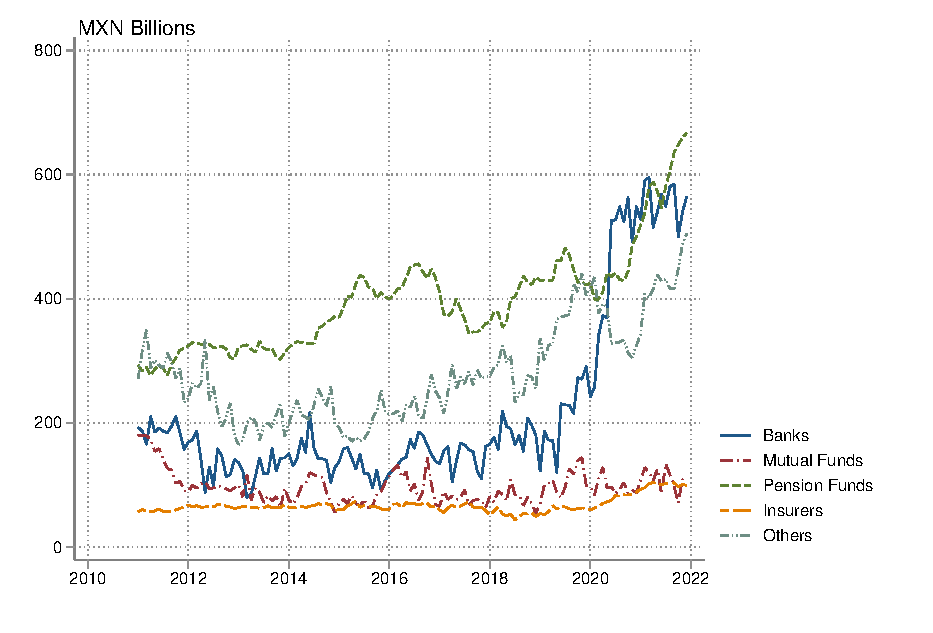
\includegraphics[width=1\textwidth,height=.3\textheight]{../Figures/Flows/bndgroups} \\
				\end{center}
%				\vspace{-0.4cm}
				\fignotes{This figure shows the net holdings of fixed-rate Mexican sovereign bonds (bonos) by type of domestic investor from January 2011 to \lastobsflwbdm.}
			\end{minipage}
		\end{center}
	\end{figure}
\end{document}
% trim = {<left> <lower> <right> <upper>}
%\pagebreak[4]

%\begin{landscape}
%	\documentclass{article}
\usepackage[margin=1in]{geometry}
\usepackage{graphicx}
\usepackage[outdir=./]{epstopdf}  					% Avoids errors when input figures
\usepackage[labelsep=period,labelfont=bf]{caption}
\usepackage{subcaption}
\usepackage{pdflscape}
\usepackage{afterpage}
%% Personalized Macros
% Table of Contents, Tables, Subcaptions, Track Changes, Footnotes

%---------------------------------------------------------------
% Table of Contents
%---------------------------------------------------------------

% Link to ToC from section
\newcommand{\gototoc}{\vspace{-2cm} \null\hfill [\hyperlink{toc}{Go2ToC}] \newline}

% Link back to section from ToC
\newcommand{\maketoc}{
	\hypertarget{toc}{}
	\newpage
	\tableofcontents
	\vspace{2.5\bigskipamount} }

% Box with bullets for tasks to do in a section
\newenvironment{boxeditems}
	{\begin{tabular}{|p{\linewidth}|}
	\hline
	\begin{itemize}
	}
	{
	\end{itemize}
	\\ \hline
	\end{tabular} \\
	}

%---------------------------------------------------------------
% Tables
%---------------------------------------------------------------

% Estout Commands following Jörg Weber
\newcommand{\sym}[1]{\rlap{#1}}

\let\estinput=\input	% define new input command to flatten the document

\newcommand{\estauto}[2]{
	\newcolumntype{C}{>{\centering\arraybackslash}X}
	\vspace{.75ex}{
%		\begin{tabularx}{1.4\textwidth}{l*{#2}C}
		\begin{tabularx}{0.95\linewidth}{l*{#2}C}
			\toprule
			\estinput{#1}
			\\ \bottomrule
			\addlinespace[.75ex]
		\end{tabularx}
	}
}

% Allow line breaks with \\ in specialcells
\newcommand{\specialcell}[2][c]{\begin{tabular}[#1]{@{}c@{}}#2\end{tabular}}

%---------------------------------------------------------------
% Subcaptions
%---------------------------------------------------------------

% Notes after figures following Jörg Weber
\newcommand{\figtext}[1]{
	\vspace{-1ex}
	\captionsetup{justification=justified,font=footnotesize}
	\caption*{#1}
%	\captionsetup{justification=raggedright,singlelinecheck=false,font=footnotesize}
%	\caption*{\hspace{6pt}\hangindent=1.5em #1}
}

\newcommand{\fignote}[1]{\figtext{\emph{Note:~}~#1}}
\newcommand{\fignotes}[1]{\figtext{\emph{Notes:~}~#1}}

% Notes after tables
\newcommand{\tabnote}[1]{
	\begin{tablenotes}[para,flushleft]
		\footnotesize \emph{Notes:~}~#1
	\end{tablenotes}
}

%---------------------------------------------------------------
% Track Changes
%---------------------------------------------------------------

% Highlight changes in revised version with color
\newcommand{\textchange}[1]{\iftoggle{revised}{\textcolor{blue}{#1}}{#1}}

%---------------------------------------------------------------
% Footnotes
%---------------------------------------------------------------

%% Change the look of foonote indicators
%\makeatletter
%\let \@makefntextorig \@makefntext
%\newcommand{\@makefntextcustom}[1]{%
%	\thefootnote.\enskip #1%
%}
%\renewcommand{\@makefntext}[1]{\@makefntextcustom{#1}}
%\makeatother
%
%% Change the look of endnote indicators
%\renewcommand{\makeenmark}{\hbox{$^{\theenmark}$}}
%\makeatletter
%\def\enoteformat{%
%	\rightskip\z@ \leftskip\z@ \parindent=1.8em
%	\leavevmode{\setbox\z@=\lastbox}\llap{\theenmark.\enskip}%
%}
%\makeatother			   % Personalized commands
%% Personalized Macros
% Variable Definitions, Equations

%---------------------------------------------------------------
% Variable Definitions
%---------------------------------------------------------------
\providecommand{\tiie}{TIIE28D}
\providecommand{\lastobs}{December 2021}
\providecommand{\lastobsfx}{November 2021}
\providecommand{\lastobsflwbdm}{December 2021}
\providecommand{\lastobsflwtic}{August 2021}
\providecommand{\idxt}{t}
\providecommand{\idxh}{h}
\providecommand{\idxi}{i}
\providecommand{\idxsfwd}{\idxt+\idxh}
\providecommand{\idxslag}{\idxt-1}
\providecommand{\yld}{y}
\providecommand{\ctrls}{z}
\providecommand{\hld}{H}
\providecommand{\depvar}{\Delta \yld_{\idxt}}
\providecommand{\mps}{\Delta x_{\idxt}}
\providecommand{\depvarclean}{\depvar^{*}}
\providecommand{\mpsclean}{\mps^{*}}
\providecommand{\paramB}{\beta}
\providecommand{\intrcpt}{\paramB_{0}}
\providecommand{\slopetrgt}{\paramB_{1}}
\providecommand{\slopepath}{\paramB_{2}}
\providecommand{\assets}{X}
\providecommand{\factors}{F}
\providecommand{\loadings}{\Lambda}
\providecommand{\rotated}{Z}
\providecommand{\rmatrix}{U}
\providecommand{\rtdone}{\rotated_{1}}
\providecommand{\rtdtwo}{\rotated_{2}}
\providecommand{\rtdonereg}{Target_{\idxt}}
\providecommand{\rtdtworeg}{Path_{\idxt}}
\providecommand{\lagidx}{j}
\providecommand{\lagorder}{p}
\providecommand{\lagparam}{\gamma}   %\alpha
\providecommand{\lagoper}{L}
\providecommand{\depvarflw}{\Delta \hld_{\idxt}}
\providecommand{\flows}{w_{\idxt}}
\providecommand{\flowslag}{w_{\idxt - \lagidx}}
\providecommand{\lagsum}{\sum_{\lagidx = 1}^{\lagorder} \lagparam_{\lagidx} \flowslag}
\providecommand{\lagsumh}{\sum_{\lagidx = 1}^{\lagorder} \lagparam^{\lagidx}_\idxh \flowslag}
\providecommand{\dimobs}{T}
\providecommand{\dimassets}{n}
\providecommand{\dimfactors}{k}
\providecommand{\dimnull}{\dimfactors_{0}}
\providecommand{\dimsassets}{\dimobs \times \dimassets}
\providecommand{\dimsfactors}{\dimobs \times \dimfactors}
\providecommand{\dimsloadings}{\dimfactors \times \dimassets}
\providecommand{\errorreg}{\varepsilon_{\idxt}}
\providecommand{\errorfac}{\zeta}
\providecommand{\errorflows}{\nu_{\idxt}}
\providecommand{\Rsqrt}{R^{2}}

\providecommand{\dpv}{y}
\providecommand{\idv}{x}
\providecommand{\omv}{\omega}
\providecommand{\dpvstar}{\dpv^{*}}
\providecommand{\idvstar}{\idv^{*}}
\providecommand{\jobs}{Jobs}
\providecommand{\errortrue}{\varepsilon}
\providecommand{\errormix}{\tau}
\providecommand{\melhs}{\nu}
\providecommand{\merhs}{u}
\providecommand{\mean}{\mu}
\providecommand{\covar}{\sigma}
\providecommand{\corr}{\rho}
\providecommand{\var}{\covar^{2}}
\providecommand{\meanE}{\mean_{\errortrue}}
\providecommand{\meanU}{\mean_{\merhs}}
\providecommand{\meanV}{\mean_{\melhs}}
\providecommand{\varE}{\var_{\errortrue}}
\providecommand{\varU}{\var_{\merhs}}
\providecommand{\varV}{\var_{\melhs}}
\providecommand{\varX}{\var_{\idv}}
\providecommand{\varXstar}{\var_{\idvstar}}
\providecommand{\covarEX}{\covar_{\errortrue \idvstar}}
\providecommand{\covarUE}{\covar_{\merhs \errortrue}}
\providecommand{\covarVE}{\covar_{\melhs \errortrue}}
\providecommand{\covarUX}{\covar_{\merhs \idvstar}}
\providecommand{\covarUY}{\covar_{\merhs \dpvstar}}
\providecommand{\covarVX}{\covar_{\melhs \idvstar}}
\providecommand{\covarVY}{\covar_{\melhs \dpvstar}}
\providecommand{\covarUV}{\covar_{\merhs \melhs}}
\providecommand{\covarWXe}{\covar_{\omv \idv}}
\providecommand{\covarVXe}{\covar_{\melhs \idv}}
\providecommand{\corrUV}{\corr_{\merhs \melhs}}
\providecommand{\corrUX}{\corr_{\merhs \idvstar}}
\providecommand{\corrUY}{\corr_{\merhs \dpvstar}}
\providecommand{\corrVX}{\corr_{\melhs \idvstar}}
\providecommand{\corrVY}{\corr_{\melhs \dpvstar}}
\providecommand{\paramG}{\gamma}
\providecommand{\estimB}{\hat{\paramB}}
\providecommand{\paramSE}{\varE}
\providecommand{\estimSE}{\hat{\paramSE}}
\providecommand{\paramAVB}{s}
\providecommand{\estimAVB}{\hat{\paramAVB}}
\providecommand{\attnfactor}{\lambda}
\providecommand{\plim}{\mathrm{plim}}

\providecommand{\reg}{\delta}
\providecommand{\regVonX}{\reg_{\melhs \idv}}
\providecommand{\regWonX}{\reg_{\omv \idv}}
\providecommand{\regWonXstar}{\reg_{\omv \idvstar}}

%---------------------------------------------------------------
% Equations
%---------------------------------------------------------------
\newcommand{\eqOneFac}{\depvar = \intrcpt + \slopetrgt \mps + \errorreg}
\newcommand{\eqOneFacOV}{\depvar = \intrcpt + \slopetrgt PRS_{\idxt} + \paramB_{2} \Delta VIX_{\idxt} + \paramB_{3} \Delta USY_{\idxt} + \paramB_{4} WTI_{\idxt} + \paramB_{5} \jobs_{\idxt} + \errorreg}
\newcommand{\eqTwoFacP}{\depvar = \intrcpt + \slopetrgt \rtdonereg + \slopepath \rtdtworeg + \errorreg}
\newcommand{\eqTwoFacF}{\depvarflw = \intrcpt + \slopetrgt \rtdonereg + \slopepath \rtdtworeg + \errorreg}
\newcommand{\eqPCA}{\assets = \factors \loadings + \errorfac}
\newcommand{\eqRotation}{\rotated = \factors \, \rmatrix}
\newcommand{\eqFlows}{\flows = \intrcpt + \slopetrgt \rtdonereg + \slopepath \rtdtworeg + \lagsum + \eta^{'} \ctrls_{\idxslag} + \errorflows}
%\newcommand{\eqLagPoly}{\lagsum = 1 - \lagparam_{1} \lagoper - \lagparam_{2} \lagoper^{2} - \ldots - \lagparam_{\lagorder} \lagoper^{\lagorder}}
\newcommand{\eqAsym}{\yld_{\idxt} = \intrcpt + \paramB_{1} \rtdonereg \mathds{1} \left(\rtdonereg > 0 \right) + \paramB_{2} \rtdonereg \mathds{1} \left(\rtdonereg < 0 \right) \\ + \paramB_{3} \rtdtworeg \mathds{1} \left(\rtdtworeg > 0 \right) + \paramB_{4} \rtdtworeg \mathds{1} \left(\rtdtworeg < 0 \right) + \errorreg}

\newcommand{\eqDGP}{\dpvstar &= \paramB \idvstar + \errortrue}
\newcommand{\eqDGPme}{\dpv = \paramB \idv + \errormix = \paramB \idv + \eqErrormix}
\newcommand{\eqDGPov}{\dpvstar = \paramB \idvstar + \paramG \omv +  \errortrue}
\newcommand{\eqMEdpv}{\dpv &= \dpvstar + \melhs}
\newcommand{\eqMEidv}{\idv &= \idvstar + \merhs}
\newcommand{\eqAtten}{\attnfactor = \frac{\varXstar}{\varXstar + \varU}}
\newcommand{\eqAttenInLine}{\attnfactor = \varXstar / \left(\varXstar + \varU\right) }
\newcommand{\eqErrormix}{\errortrue - \paramB \merhs + \melhs}

\newcommand{\eqPlimBstd}{\plim \left( \estimB \right) = \frac{cov(\idv, \dpvstar)}{var(\idv)} = \frac{cov(\idvstar + \merhs, \paramB \idvstar + \errortrue)}{var(\idvstar + \merhs)} = \paramB \frac{\varXstar}{\varXstar + \varU} = \paramB \attnfactor}
\newcommand{\eqPlimBstdshort}{\plim (\estimB) = \paramB \attnfactor}

%\newcommand{\eqPlimSstd}{\plim \left( \estimAVB \right) = \plim \left( \frac{\estimSE}{\hat{\varX}} \right) = \frac{\varE + (1-\attnfactor)^{2} \paramB^{2} \varXstar + \attnfactor^{2} \paramB^{2} \varU}{\varXstar + \varU} = \attnfactor \paramAVB + \attnfactor(1 - \attnfactor) \paramB^{2}}
\newcommand{\eqPlimSstd}{\plim \left( \estimAVB \right) = \attnfactor \paramAVB + \attnfactor(1 - \attnfactor) \paramB^{2}}

\newcommand{\eqPlimBnew}{\plim \left( \estimB \right) 
	= \frac{cov(\idv, \dpv)}{var(\idv)} 
	= \frac{cov(\idvstar + \merhs, \paramB \idvstar + \paramG \omv + \errortrue)}{var(\idvstar + \merhs)} 
	= \frac{\paramB \varXstar + \paramG \covarWXe}{\varXstar + \varU}  }

\newcommand{\eqPlimBbias}{\plim \left( \estimB \right)
	= \paramB \frac{\varXstar}{\varX} + \paramG \frac{\covarWXe}{\varX}
	= \paramB \attnfactor + \paramG \regWonX}

\providecommand{\errordepvar}{e_{y}}
\providecommand{\errormps}{e_{x}}
\newcommand{\eqMEdepvar}{\depvar &= \depvarclean + \errordepvar}
\newcommand{\eqMEmps}{\mps &= \mpsclean + \errormps}

\newcommand{\eqLPrhs}{\alpha_{\idxh} + \beta^{1}_{\idxh} \; \rtdonereg +  \beta^{2}_{\idxh} \; \rtdtworeg + \eta^{'}_{\idxh} \ctrls_{\idxslag}  + u_{\idxsfwd}}

\newcommand{\eqLPprices}{\yld_{\idxsfwd} - \yld_{\idxslag} = \eqLPrhs} 

\newcommand{\eqLPflows}{\hld_{\idxsfwd} - \hld_{\idxslag} = \eqLPrhs} 
% \gamma_{\idxh} \Delta \yld_{\idxslag} 
%\alpha_{\idxh} + \beta^{1}_{\idxh} \; \rtdonereg +  \beta^{2}_{\idxh} \; \rtdtworeg + \lagsumh + \eta_{\idxh} \ctrls_{\idxslag}  + u_{\idxsfwd}

\newcommand{\eqLP}{\yld_{\idxsfwd} - \yld_{\idxslag} = \alpha_{\idxh} + \gamma_{\idxh} \mps + u_{\idxsfwd}} 			    % Personalized commands
%\pagestyle{empty}

\begin{document}
	\afterpage{
	\begin{landscape}
	\begin{figure}[tbph]
		\caption{Response of Bonos Flows to Target and Path Surprises} \label{fig:LPBondsInstit}
		\begin{center}
			\begin{minipage}{\linewidth}
				\begin{center}
					\begin{subfigure}[t]{\linewidth}
						\includegraphics[trim={0.3cm 0.23cm 0.3cm 0.23cm},clip,height=0.33\textheight,width=\linewidth]{../Figures/LPs/Target/Bonds/Target11BondsInstit1.eps} \\
%						\includegraphics[trim={0.3cm 0.23cm 0.3cm 0.23cm},clip,height=0.33\textheight,width=\linewidth]{../Target/Bonds/Target11BondsInstit1.eps} \\
						\vspace{-0.35cm}
						\caption{Target  Surprise} \label{subfig:Target11BondsInstit}
						\vspace{0.4cm}
					\end{subfigure}
				
					\vspace{0.1cm}
					
					\begin{subfigure}[t]{\linewidth}
						\includegraphics[trim={0.3cm 0.23cm 0.3cm 0.23cm},clip,height=0.33\textheight,width=\linewidth]{../Figures/LPs/Path/Bonds/Path11BondsInstit1.eps} \\
%						\includegraphics[trim={0.3cm 0.23cm 0.3cm 0.23cm},clip,height=0.33\textheight,width=\linewidth]{../Path/Bonds/Path11BondsInstit1.eps} \\
						\vspace{-0.35cm}
						\caption{Path Surprise} \label{subfig:Path11BondsInstit}
					\end{subfigure}
					\vspace{-0.45cm}
				\end{center}
				\fignotes{This figure plots the coefficient estimates and 95\% confidence intervals for 1 basis point target and path tightening surprises for bonos flows from day \(t - 1\) to day \(t + \idxh\), where \(t\) is a day with a monetary policy announcement and \(\idxh = 0, 1, \ldots, 30\). An arrow in the vertical axis indicates the contemporaneous effect (when \(\idxh = 0\)). The surprises are equal to the target and path surprises (obtained with intraday data) on announcement days and zero otherwise. The sample includes all regular monetary policy announcements from January 2011 to \lastobsflwbdm. The 95\% confidence bands are based on robust standard errors.}
			\end{minipage}
		\end{center}
	\end{figure}
	\end{landscape}
	}
\end{document}
% trim = {<left> <lower> <right> <upper>}
%	\documentclass{article}
\usepackage[margin=1in]{geometry}
\usepackage{graphicx}
\usepackage[outdir=./]{epstopdf}  					% Avoids errors when input figures
\usepackage[labelsep=period,labelfont=bf]{caption}
\usepackage{subcaption}
\usepackage{pdflscape}
\usepackage{afterpage}
%% Personalized Macros
% Table of Contents, Tables, Subcaptions, Track Changes, Footnotes

%---------------------------------------------------------------
% Table of Contents
%---------------------------------------------------------------

% Link to ToC from section
\newcommand{\gototoc}{\vspace{-2cm} \null\hfill [\hyperlink{toc}{Go2ToC}] \newline}

% Link back to section from ToC
\newcommand{\maketoc}{
	\hypertarget{toc}{}
	\newpage
	\tableofcontents
	\vspace{2.5\bigskipamount} }

% Box with bullets for tasks to do in a section
\newenvironment{boxeditems}
	{\begin{tabular}{|p{\linewidth}|}
	\hline
	\begin{itemize}
	}
	{
	\end{itemize}
	\\ \hline
	\end{tabular} \\
	}

%---------------------------------------------------------------
% Tables
%---------------------------------------------------------------

% Estout Commands following Jörg Weber
\newcommand{\sym}[1]{\rlap{#1}}

\let\estinput=\input	% define new input command to flatten the document

\newcommand{\estauto}[2]{
	\newcolumntype{C}{>{\centering\arraybackslash}X}
	\vspace{.75ex}{
%		\begin{tabularx}{1.4\textwidth}{l*{#2}C}
		\begin{tabularx}{0.95\linewidth}{l*{#2}C}
			\toprule
			\estinput{#1}
			\\ \bottomrule
			\addlinespace[.75ex]
		\end{tabularx}
	}
}

% Allow line breaks with \\ in specialcells
\newcommand{\specialcell}[2][c]{\begin{tabular}[#1]{@{}c@{}}#2\end{tabular}}

%---------------------------------------------------------------
% Subcaptions
%---------------------------------------------------------------

% Notes after figures following Jörg Weber
\newcommand{\figtext}[1]{
	\vspace{-1ex}
	\captionsetup{justification=justified,font=footnotesize}
	\caption*{#1}
%	\captionsetup{justification=raggedright,singlelinecheck=false,font=footnotesize}
%	\caption*{\hspace{6pt}\hangindent=1.5em #1}
}

\newcommand{\fignote}[1]{\figtext{\emph{Note:~}~#1}}
\newcommand{\fignotes}[1]{\figtext{\emph{Notes:~}~#1}}

% Notes after tables
\newcommand{\tabnote}[1]{
	\begin{tablenotes}[para,flushleft]
		\footnotesize \emph{Notes:~}~#1
	\end{tablenotes}
}

%---------------------------------------------------------------
% Track Changes
%---------------------------------------------------------------

% Highlight changes in revised version with color
\newcommand{\textchange}[1]{\iftoggle{revised}{\textcolor{blue}{#1}}{#1}}

%---------------------------------------------------------------
% Footnotes
%---------------------------------------------------------------

%% Change the look of foonote indicators
%\makeatletter
%\let \@makefntextorig \@makefntext
%\newcommand{\@makefntextcustom}[1]{%
%	\thefootnote.\enskip #1%
%}
%\renewcommand{\@makefntext}[1]{\@makefntextcustom{#1}}
%\makeatother
%
%% Change the look of endnote indicators
%\renewcommand{\makeenmark}{\hbox{$^{\theenmark}$}}
%\makeatletter
%\def\enoteformat{%
%	\rightskip\z@ \leftskip\z@ \parindent=1.8em
%	\leavevmode{\setbox\z@=\lastbox}\llap{\theenmark.\enskip}%
%}
%\makeatother			   % Personalized commands
%% Personalized Macros
% Variable Definitions, Equations

%---------------------------------------------------------------
% Variable Definitions
%---------------------------------------------------------------
\providecommand{\tiie}{TIIE28D}
\providecommand{\lastobs}{December 2021}
\providecommand{\lastobsfx}{November 2021}
\providecommand{\lastobsflwbdm}{December 2021}
\providecommand{\lastobsflwtic}{August 2021}
\providecommand{\idxt}{t}
\providecommand{\idxh}{h}
\providecommand{\idxi}{i}
\providecommand{\idxsfwd}{\idxt+\idxh}
\providecommand{\idxslag}{\idxt-1}
\providecommand{\yld}{y}
\providecommand{\ctrls}{z}
\providecommand{\hld}{H}
\providecommand{\depvar}{\Delta \yld_{\idxt}}
\providecommand{\mps}{\Delta x_{\idxt}}
\providecommand{\depvarclean}{\depvar^{*}}
\providecommand{\mpsclean}{\mps^{*}}
\providecommand{\paramB}{\beta}
\providecommand{\intrcpt}{\paramB_{0}}
\providecommand{\slopetrgt}{\paramB_{1}}
\providecommand{\slopepath}{\paramB_{2}}
\providecommand{\assets}{X}
\providecommand{\factors}{F}
\providecommand{\loadings}{\Lambda}
\providecommand{\rotated}{Z}
\providecommand{\rmatrix}{U}
\providecommand{\rtdone}{\rotated_{1}}
\providecommand{\rtdtwo}{\rotated_{2}}
\providecommand{\rtdonereg}{Target_{\idxt}}
\providecommand{\rtdtworeg}{Path_{\idxt}}
\providecommand{\lagidx}{j}
\providecommand{\lagorder}{p}
\providecommand{\lagparam}{\gamma}   %\alpha
\providecommand{\lagoper}{L}
\providecommand{\depvarflw}{\Delta \hld_{\idxt}}
\providecommand{\flows}{w_{\idxt}}
\providecommand{\flowslag}{w_{\idxt - \lagidx}}
\providecommand{\lagsum}{\sum_{\lagidx = 1}^{\lagorder} \lagparam_{\lagidx} \flowslag}
\providecommand{\lagsumh}{\sum_{\lagidx = 1}^{\lagorder} \lagparam^{\lagidx}_\idxh \flowslag}
\providecommand{\dimobs}{T}
\providecommand{\dimassets}{n}
\providecommand{\dimfactors}{k}
\providecommand{\dimnull}{\dimfactors_{0}}
\providecommand{\dimsassets}{\dimobs \times \dimassets}
\providecommand{\dimsfactors}{\dimobs \times \dimfactors}
\providecommand{\dimsloadings}{\dimfactors \times \dimassets}
\providecommand{\errorreg}{\varepsilon_{\idxt}}
\providecommand{\errorfac}{\zeta}
\providecommand{\errorflows}{\nu_{\idxt}}
\providecommand{\Rsqrt}{R^{2}}

\providecommand{\dpv}{y}
\providecommand{\idv}{x}
\providecommand{\omv}{\omega}
\providecommand{\dpvstar}{\dpv^{*}}
\providecommand{\idvstar}{\idv^{*}}
\providecommand{\jobs}{Jobs}
\providecommand{\errortrue}{\varepsilon}
\providecommand{\errormix}{\tau}
\providecommand{\melhs}{\nu}
\providecommand{\merhs}{u}
\providecommand{\mean}{\mu}
\providecommand{\covar}{\sigma}
\providecommand{\corr}{\rho}
\providecommand{\var}{\covar^{2}}
\providecommand{\meanE}{\mean_{\errortrue}}
\providecommand{\meanU}{\mean_{\merhs}}
\providecommand{\meanV}{\mean_{\melhs}}
\providecommand{\varE}{\var_{\errortrue}}
\providecommand{\varU}{\var_{\merhs}}
\providecommand{\varV}{\var_{\melhs}}
\providecommand{\varX}{\var_{\idv}}
\providecommand{\varXstar}{\var_{\idvstar}}
\providecommand{\covarEX}{\covar_{\errortrue \idvstar}}
\providecommand{\covarUE}{\covar_{\merhs \errortrue}}
\providecommand{\covarVE}{\covar_{\melhs \errortrue}}
\providecommand{\covarUX}{\covar_{\merhs \idvstar}}
\providecommand{\covarUY}{\covar_{\merhs \dpvstar}}
\providecommand{\covarVX}{\covar_{\melhs \idvstar}}
\providecommand{\covarVY}{\covar_{\melhs \dpvstar}}
\providecommand{\covarUV}{\covar_{\merhs \melhs}}
\providecommand{\covarWXe}{\covar_{\omv \idv}}
\providecommand{\covarVXe}{\covar_{\melhs \idv}}
\providecommand{\corrUV}{\corr_{\merhs \melhs}}
\providecommand{\corrUX}{\corr_{\merhs \idvstar}}
\providecommand{\corrUY}{\corr_{\merhs \dpvstar}}
\providecommand{\corrVX}{\corr_{\melhs \idvstar}}
\providecommand{\corrVY}{\corr_{\melhs \dpvstar}}
\providecommand{\paramG}{\gamma}
\providecommand{\estimB}{\hat{\paramB}}
\providecommand{\paramSE}{\varE}
\providecommand{\estimSE}{\hat{\paramSE}}
\providecommand{\paramAVB}{s}
\providecommand{\estimAVB}{\hat{\paramAVB}}
\providecommand{\attnfactor}{\lambda}
\providecommand{\plim}{\mathrm{plim}}

\providecommand{\reg}{\delta}
\providecommand{\regVonX}{\reg_{\melhs \idv}}
\providecommand{\regWonX}{\reg_{\omv \idv}}
\providecommand{\regWonXstar}{\reg_{\omv \idvstar}}

%---------------------------------------------------------------
% Equations
%---------------------------------------------------------------
\newcommand{\eqOneFac}{\depvar = \intrcpt + \slopetrgt \mps + \errorreg}
\newcommand{\eqOneFacOV}{\depvar = \intrcpt + \slopetrgt PRS_{\idxt} + \paramB_{2} \Delta VIX_{\idxt} + \paramB_{3} \Delta USY_{\idxt} + \paramB_{4} WTI_{\idxt} + \paramB_{5} \jobs_{\idxt} + \errorreg}
\newcommand{\eqTwoFacP}{\depvar = \intrcpt + \slopetrgt \rtdonereg + \slopepath \rtdtworeg + \errorreg}
\newcommand{\eqTwoFacF}{\depvarflw = \intrcpt + \slopetrgt \rtdonereg + \slopepath \rtdtworeg + \errorreg}
\newcommand{\eqPCA}{\assets = \factors \loadings + \errorfac}
\newcommand{\eqRotation}{\rotated = \factors \, \rmatrix}
\newcommand{\eqFlows}{\flows = \intrcpt + \slopetrgt \rtdonereg + \slopepath \rtdtworeg + \lagsum + \eta^{'} \ctrls_{\idxslag} + \errorflows}
%\newcommand{\eqLagPoly}{\lagsum = 1 - \lagparam_{1} \lagoper - \lagparam_{2} \lagoper^{2} - \ldots - \lagparam_{\lagorder} \lagoper^{\lagorder}}
\newcommand{\eqAsym}{\yld_{\idxt} = \intrcpt + \paramB_{1} \rtdonereg \mathds{1} \left(\rtdonereg > 0 \right) + \paramB_{2} \rtdonereg \mathds{1} \left(\rtdonereg < 0 \right) \\ + \paramB_{3} \rtdtworeg \mathds{1} \left(\rtdtworeg > 0 \right) + \paramB_{4} \rtdtworeg \mathds{1} \left(\rtdtworeg < 0 \right) + \errorreg}

\newcommand{\eqDGP}{\dpvstar &= \paramB \idvstar + \errortrue}
\newcommand{\eqDGPme}{\dpv = \paramB \idv + \errormix = \paramB \idv + \eqErrormix}
\newcommand{\eqDGPov}{\dpvstar = \paramB \idvstar + \paramG \omv +  \errortrue}
\newcommand{\eqMEdpv}{\dpv &= \dpvstar + \melhs}
\newcommand{\eqMEidv}{\idv &= \idvstar + \merhs}
\newcommand{\eqAtten}{\attnfactor = \frac{\varXstar}{\varXstar + \varU}}
\newcommand{\eqAttenInLine}{\attnfactor = \varXstar / \left(\varXstar + \varU\right) }
\newcommand{\eqErrormix}{\errortrue - \paramB \merhs + \melhs}

\newcommand{\eqPlimBstd}{\plim \left( \estimB \right) = \frac{cov(\idv, \dpvstar)}{var(\idv)} = \frac{cov(\idvstar + \merhs, \paramB \idvstar + \errortrue)}{var(\idvstar + \merhs)} = \paramB \frac{\varXstar}{\varXstar + \varU} = \paramB \attnfactor}
\newcommand{\eqPlimBstdshort}{\plim (\estimB) = \paramB \attnfactor}

%\newcommand{\eqPlimSstd}{\plim \left( \estimAVB \right) = \plim \left( \frac{\estimSE}{\hat{\varX}} \right) = \frac{\varE + (1-\attnfactor)^{2} \paramB^{2} \varXstar + \attnfactor^{2} \paramB^{2} \varU}{\varXstar + \varU} = \attnfactor \paramAVB + \attnfactor(1 - \attnfactor) \paramB^{2}}
\newcommand{\eqPlimSstd}{\plim \left( \estimAVB \right) = \attnfactor \paramAVB + \attnfactor(1 - \attnfactor) \paramB^{2}}

\newcommand{\eqPlimBnew}{\plim \left( \estimB \right) 
	= \frac{cov(\idv, \dpv)}{var(\idv)} 
	= \frac{cov(\idvstar + \merhs, \paramB \idvstar + \paramG \omv + \errortrue)}{var(\idvstar + \merhs)} 
	= \frac{\paramB \varXstar + \paramG \covarWXe}{\varXstar + \varU}  }

\newcommand{\eqPlimBbias}{\plim \left( \estimB \right)
	= \paramB \frac{\varXstar}{\varX} + \paramG \frac{\covarWXe}{\varX}
	= \paramB \attnfactor + \paramG \regWonX}

\providecommand{\errordepvar}{e_{y}}
\providecommand{\errormps}{e_{x}}
\newcommand{\eqMEdepvar}{\depvar &= \depvarclean + \errordepvar}
\newcommand{\eqMEmps}{\mps &= \mpsclean + \errormps}

\newcommand{\eqLPrhs}{\alpha_{\idxh} + \beta^{1}_{\idxh} \; \rtdonereg +  \beta^{2}_{\idxh} \; \rtdtworeg + \eta^{'}_{\idxh} \ctrls_{\idxslag}  + u_{\idxsfwd}}

\newcommand{\eqLPprices}{\yld_{\idxsfwd} - \yld_{\idxslag} = \eqLPrhs} 

\newcommand{\eqLPflows}{\hld_{\idxsfwd} - \hld_{\idxslag} = \eqLPrhs} 
% \gamma_{\idxh} \Delta \yld_{\idxslag} 
%\alpha_{\idxh} + \beta^{1}_{\idxh} \; \rtdonereg +  \beta^{2}_{\idxh} \; \rtdtworeg + \lagsumh + \eta_{\idxh} \ctrls_{\idxslag}  + u_{\idxsfwd}

\newcommand{\eqLP}{\yld_{\idxsfwd} - \yld_{\idxslag} = \alpha_{\idxh} + \gamma_{\idxh} \mps + u_{\idxsfwd}} 			    % Personalized commands
%\pagestyle{empty}

\begin{document}
	\afterpage{
	\begin{landscape}
	\begin{figure}[tbph]
		\caption{Response of Bonos Flows to Target and Path Factors (cont.)} \label{fig:LPBondsOther}
		\begin{center}
			\begin{minipage}{\linewidth}
				\begin{center}
					\begin{subfigure}[t]{\linewidth}
%						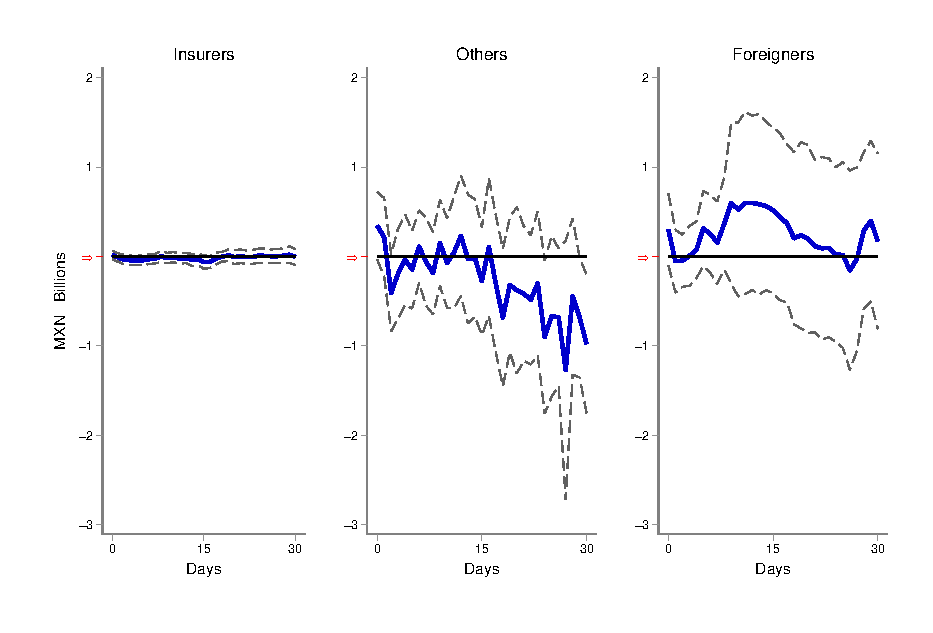
\includegraphics[trim={0.3cm 0.23cm 0.3cm 0.23cm},clip,height=0.33\textheight,width=\linewidth]{../Figures/LPs/Target/Bonds/Target11BondsInstit2.eps} \\
						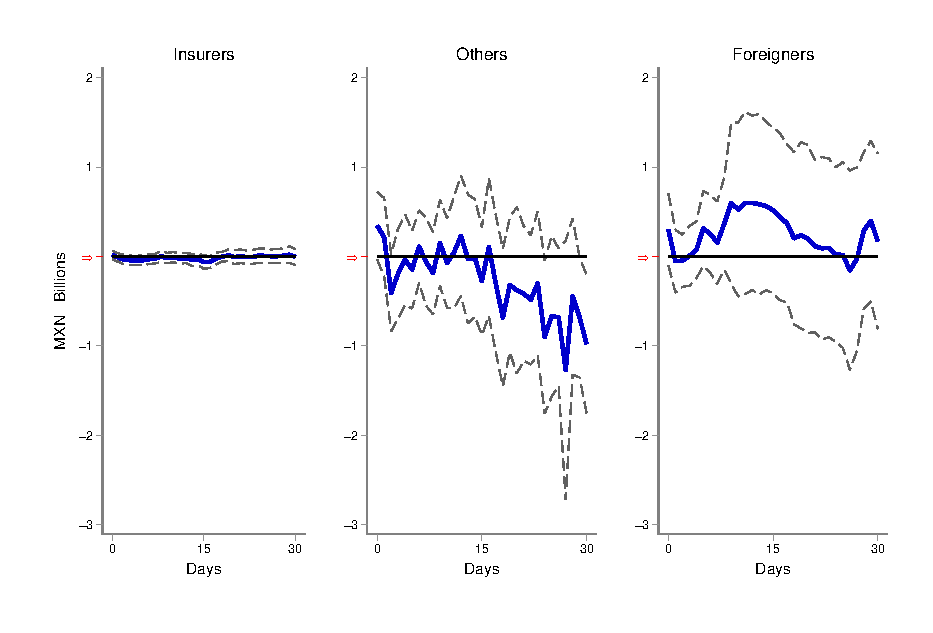
\includegraphics[trim={0.3cm 0.23cm 0.3cm 0.23cm},clip,height=0.33\textheight,width=\linewidth]{../Figures/LPs/Target/Bonds/Target11BondsInstit2.eps} \\
						\vspace{-0.35cm}
						\caption{Target  Surprise} \label{subfig:Target11BondsOther}
						\vspace{0.4cm}
					\end{subfigure}
				
					\vspace{0.1cm}
					
					\begin{subfigure}[t]{\linewidth}
%						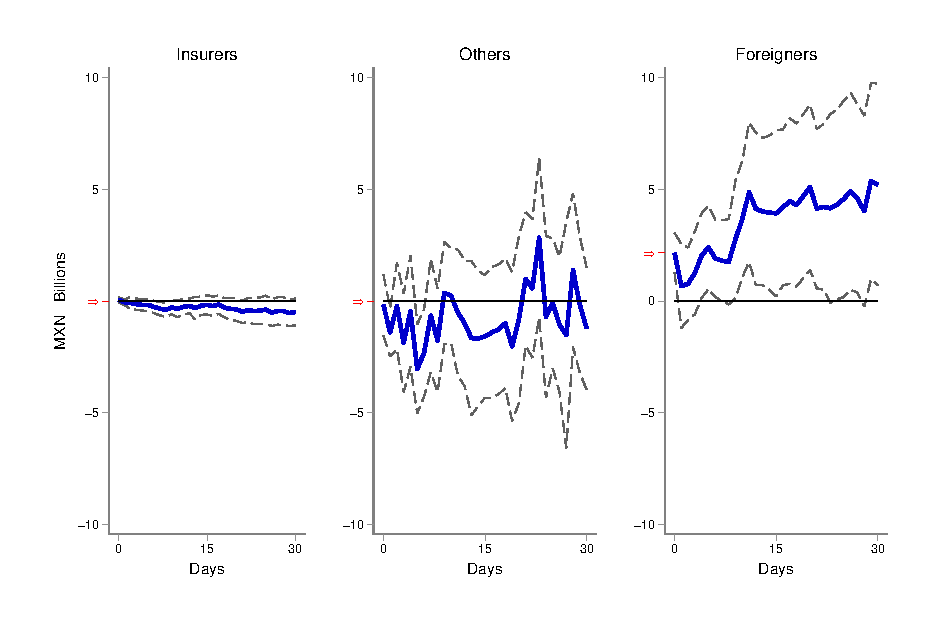
\includegraphics[trim={0.3cm 0.23cm 0.3cm 0.23cm},clip,height=0.33\textheight,width=\linewidth]{../Figures/LPs/Path/Bonds/Path11BondsInstit2.eps} \\
						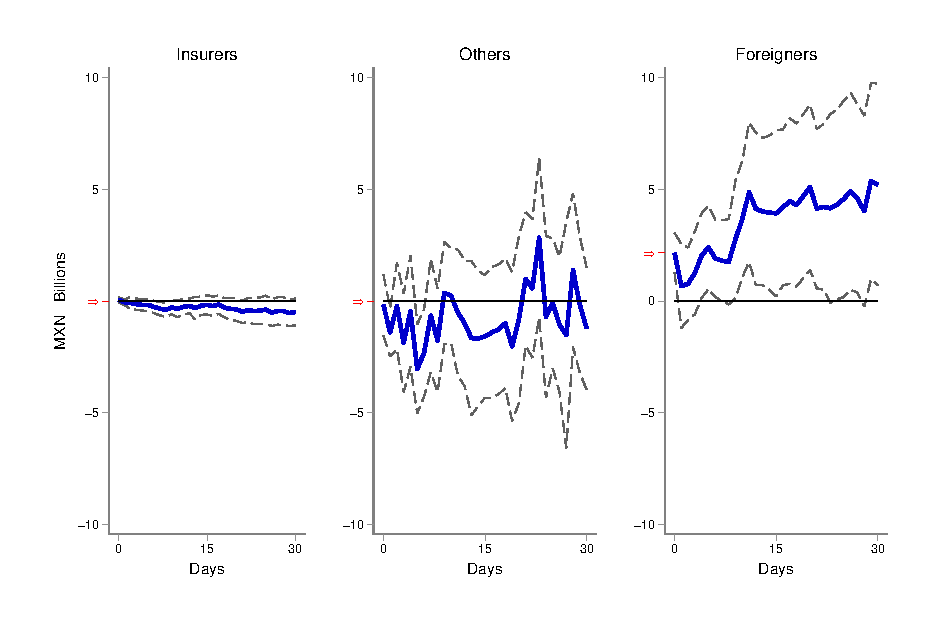
\includegraphics[trim={0.3cm 0.23cm 0.3cm 0.23cm},clip,height=0.33\textheight,width=\linewidth]{../Figures/LPs/Path/Bonds/Path11BondsInstit2.eps} \\
						\vspace{-0.35cm}
						\caption{Path Surprise} \label{subfig:Path11BondsOther}
					\end{subfigure}
					\vspace{-0.45cm}
				\end{center}
				\fignotes{This figure plots the coefficient estimates and 95\% confidence intervals for 1 basis point target and path tightening surprises for bonos flows from day \(t - 1\) to day \(t + \idxh\), where \(t\) is a day with a monetary policy announcement and \(\idxh = 0, 1, \ldots, 30\). An arrow in the vertical axis indicates the contemporaneous effect (when \(\idxh = 0\)). The surprises are equal to the target and path surprises (obtained with intraday data) on announcement days and zero otherwise. The sample includes all regular monetary policy announcements from January 2011 to \lastobsflwbdm. The 95\% confidence bands are based on robust standard errors.}
			\end{minipage}
		\end{center}
	\end{figure}
	\end{landscape}
	}
\end{document}
% trim = {<left> <lower> <right> <upper>}
%\end{landscape}
%\pagebreak[4]


%\documentclass[a4paper,10pt]{article}
\usepackage[labelsep=period,labelfont=bf]{caption}
\usepackage{multirow}
\usepackage{booktabs}
\usepackage{threeparttable}
\usepackage{longtable}
\usepackage{pdflscape}
\usepackage{afterpage}
\begin{document}
\afterpage{
\begin{normalsize}
\begin{landscape}
\begin{table}
\centering
\begin{threeparttable}
\caption{Tests of the Number of Factors in Monetary Policy Announcements}
\label{tab:ranktests}
\begin{tabular}{lcccccc}
\toprule
 & Frequency & \(H_{0}: k = k_{0}\) & Wald Statistic & Degrees of Freedom & \(p\)-value & Observations \\
\midrule
  &  & 0 & 29.56 & 10 & 0.001 & 56 \\
 & Intraday & 1 & 10.07 & 5 & 0.073 & 56 \\
Exchange Rate &  & 2 &  1.14 & 1 & 0.285 & 56 \\
\cmidrule(lr){2-7}
\& Yield Curve &  & 0 & 40.20 & 10 & 0.000 & 135 \\
 & Daily & 1 & 18.93 & 5 & 0.002 & 135 \\
 &  & 2 &  0.00 & 1 & 0.978 & 135 \\
\cmidrule(lr){1-7}
\multirow{4}[5]{*}{Swaps} & \multirow{2}{*}{Intraday} & 0 & 28.30 & 6 & 0.000 & 87 \\
 &  & 1 &  7.21 & 2 & 0.027 & 87 \\
\cmidrule(lr){2-7}
 & \multirow{2}{*}{Daily} & 0 & 33.06 & 6 & 0.000 & 190 \\
 &  & 1 &  9.35 & 2 & 0.009 & 190 \\
\bottomrule
\end{tabular}
\begin{tablenotes}[para,flushleft]
\footnotesize \textit{Notes:} This table reports the results from the Cragg--Donald test. \(H_{0}\) is the null hypothesis of \(k = k_{0}\) factors against the alternative of \(k > k_{0}\) factors, where \(k_{0} = 0, 1, 2\). The sample includes all regular monetary policy announcements up to \lastobs, the starting date varies based on data availability: for the exchange rate and the yield curve with intraday data, it is December 2014 (due to the 5-year yield) and with daily data is October 2006 (due to the 30-year yield); for swaps with intraday data, it is January 2011 and with daily data is January 2004. The yield curve includes 2- 5- 10- and 30-year bonds. Swaps have maturities of 3, 6, 9 and 12 months.
\end{tablenotes}
\end{threeparttable}
\end{table}
\end{landscape}
\end{normalsize}
}
\end{document}
		% \ref{tab:ranktests}
%\documentclass[a4paper,10pt]{article}
\usepackage[labelsep=period,labelfont=bf]{caption}
\usepackage{multirow}
\usepackage{booktabs}
\usepackage{longtable}
\usepackage{pdflscape}
\usepackage{afterpage}

\begin{document}
\afterpage{
\begin{normalsize}
\begin{landscape}
\begin{table}
\centering
\caption{Summary of Statements in Selected Dates}
\label{tab:statements}
\begin{tabular}{p{2.3cm} c p{17.5cm}}
\toprule
 Date & Path & Description \\
\midrule
21-Apr-2006 & \(+\) & Statement announces an easing of monetary conditions but notes that `for the foreseeable future there is no space available for further easing.' \\
26-Oct-2007 & \(-\) & Statement indicates that the risk that the sharp decline in the U.S. real estate market weakens the U.S. economy (affecting economic activity in Mexico) has increased. \\
15-Aug-2008 & \(-\) & Statement highlights that global inflationary pressures continue to rise but an improvement is foreseen in the medium term due to the prospects for lower global growth. Downside risks to the local economy have increased. \\
16-Jan-2009 & \(+\) & Statement notes `a higher than expected upward trend in inflation in the last quarter' and that `instability in financial markets continues to be a risk factor for the inflationary trend.' \\
20-Feb-2009 & \(+\) & Statement indicates that `the strong financial turmoil represents a risk to the expected inflation path, even considering the greater contraction in demand and the reduction in commodities prices.' \\
19-Jun-2009 & \(+\) & Statement indicates that `the Board considers that its easing cycle is close to an end.' \\
26-Aug-2011 & \(-\) & Statement notes that the current monetary policy stance is considered adequate but if it turns in an unnecessary tightening, the Board will reflect on the need to adjust it. \\
08-Mar-2013 & \(+\) & Statement makes clear that the 50 basis point reduction in the policy rate `does not represent the beginning of an easing cycle.' \\
25-Oct-2013 & \(+\) & Statement highlights that `no further cuts in the policy rate are appropriate in the foreseeable future.' \\
09-Feb-2017 & \(+\) & Statement highlights the effects of the tightenings in 2016 and `the ones required in 2017' to counteract inflationary pressures. \\
22-Jun-2017 & \(-\) & Statement drops reference to do `the necessary tightenings ahead' from the previous statement. \\
24-Jun-2021 & \(+\) & Statement highlights additional shocks to those expected in headline and core inflation, and notes that their expected paths in the following quarters are higher than previously estimated. \\
\bottomrule
\end{tabular}
\end{table}
\end{landscape}
\end{normalsize}
}
\end{document}
		% \ref{tab:statements}
%\documentclass[a4paper,12pt]{article}
\usepackage[labelsep=period,labelfont=bf]{caption}
\usepackage{multirow}
\usepackage{booktabs}
\usepackage{threeparttable}
\usepackage{pdflscape}
\usepackage{tabularx}
\usepackage{afterpage}
\usepackage[margin=1in]{geometry}
%% Personalized Macros
% Table of Contents, Tables, Subcaptions, Track Changes, Footnotes

%---------------------------------------------------------------
% Table of Contents
%---------------------------------------------------------------

% Link to ToC from section
\newcommand{\gototoc}{\vspace{-2cm} \null\hfill [\hyperlink{toc}{Go2ToC}] \newline}

% Link back to section from ToC
\newcommand{\maketoc}{
	\hypertarget{toc}{}
	\newpage
	\tableofcontents
	\vspace{2.5\bigskipamount} }

% Box with bullets for tasks to do in a section
\newenvironment{boxeditems}
	{\begin{tabular}{|p{\linewidth}|}
	\hline
	\begin{itemize}
	}
	{
	\end{itemize}
	\\ \hline
	\end{tabular} \\
	}

%---------------------------------------------------------------
% Tables
%---------------------------------------------------------------

% Estout Commands following Jörg Weber
\newcommand{\sym}[1]{\rlap{#1}}

\let\estinput=\input	% define new input command to flatten the document

\newcommand{\estauto}[2]{
	\newcolumntype{C}{>{\centering\arraybackslash}X}
	\vspace{.75ex}{
%		\begin{tabularx}{1.4\textwidth}{l*{#2}C}
		\begin{tabularx}{0.95\linewidth}{l*{#2}C}
			\toprule
			\estinput{#1}
			\\ \bottomrule
			\addlinespace[.75ex]
		\end{tabularx}
	}
}

% Allow line breaks with \\ in specialcells
\newcommand{\specialcell}[2][c]{\begin{tabular}[#1]{@{}c@{}}#2\end{tabular}}

%---------------------------------------------------------------
% Subcaptions
%---------------------------------------------------------------

% Notes after figures following Jörg Weber
\newcommand{\figtext}[1]{
	\vspace{-1ex}
	\captionsetup{justification=justified,font=footnotesize}
	\caption*{#1}
%	\captionsetup{justification=raggedright,singlelinecheck=false,font=footnotesize}
%	\caption*{\hspace{6pt}\hangindent=1.5em #1}
}

\newcommand{\fignote}[1]{\figtext{\emph{Note:~}~#1}}
\newcommand{\fignotes}[1]{\figtext{\emph{Notes:~}~#1}}

% Notes after tables
\newcommand{\tabnote}[1]{
	\begin{tablenotes}[para,flushleft]
		\footnotesize \emph{Notes:~}~#1
	\end{tablenotes}
}

%---------------------------------------------------------------
% Track Changes
%---------------------------------------------------------------

% Highlight changes in revised version with color
\newcommand{\textchange}[1]{\iftoggle{revised}{\textcolor{blue}{#1}}{#1}}

%---------------------------------------------------------------
% Footnotes
%---------------------------------------------------------------

%% Change the look of foonote indicators
%\makeatletter
%\let \@makefntextorig \@makefntext
%\newcommand{\@makefntextcustom}[1]{%
%	\thefootnote.\enskip #1%
%}
%\renewcommand{\@makefntext}[1]{\@makefntextcustom{#1}}
%\makeatother
%
%% Change the look of endnote indicators
%\renewcommand{\makeenmark}{\hbox{$^{\theenmark}$}}
%\makeatletter
%\def\enoteformat{%
%	\rightskip\z@ \leftskip\z@ \parindent=1.8em
%	\leavevmode{\setbox\z@=\lastbox}\llap{\theenmark.\enskip}%
%}
%\makeatother			   % Personalized commands
%% Personalized Macros
% Variable Definitions, Equations

%---------------------------------------------------------------
% Variable Definitions
%---------------------------------------------------------------
\providecommand{\tiie}{TIIE28D}
\providecommand{\lastobs}{December 2021}
\providecommand{\lastobsfx}{November 2021}
\providecommand{\lastobsflwbdm}{December 2021}
\providecommand{\lastobsflwtic}{August 2021}
\providecommand{\idxt}{t}
\providecommand{\idxh}{h}
\providecommand{\idxi}{i}
\providecommand{\idxsfwd}{\idxt+\idxh}
\providecommand{\idxslag}{\idxt-1}
\providecommand{\yld}{y}
\providecommand{\ctrls}{z}
\providecommand{\hld}{H}
\providecommand{\depvar}{\Delta \yld_{\idxt}}
\providecommand{\mps}{\Delta x_{\idxt}}
\providecommand{\depvarclean}{\depvar^{*}}
\providecommand{\mpsclean}{\mps^{*}}
\providecommand{\paramB}{\beta}
\providecommand{\intrcpt}{\paramB_{0}}
\providecommand{\slopetrgt}{\paramB_{1}}
\providecommand{\slopepath}{\paramB_{2}}
\providecommand{\assets}{X}
\providecommand{\factors}{F}
\providecommand{\loadings}{\Lambda}
\providecommand{\rotated}{Z}
\providecommand{\rmatrix}{U}
\providecommand{\rtdone}{\rotated_{1}}
\providecommand{\rtdtwo}{\rotated_{2}}
\providecommand{\rtdonereg}{Target_{\idxt}}
\providecommand{\rtdtworeg}{Path_{\idxt}}
\providecommand{\lagidx}{j}
\providecommand{\lagorder}{p}
\providecommand{\lagparam}{\gamma}   %\alpha
\providecommand{\lagoper}{L}
\providecommand{\depvarflw}{\Delta \hld_{\idxt}}
\providecommand{\flows}{w_{\idxt}}
\providecommand{\flowslag}{w_{\idxt - \lagidx}}
\providecommand{\lagsum}{\sum_{\lagidx = 1}^{\lagorder} \lagparam_{\lagidx} \flowslag}
\providecommand{\lagsumh}{\sum_{\lagidx = 1}^{\lagorder} \lagparam^{\lagidx}_\idxh \flowslag}
\providecommand{\dimobs}{T}
\providecommand{\dimassets}{n}
\providecommand{\dimfactors}{k}
\providecommand{\dimnull}{\dimfactors_{0}}
\providecommand{\dimsassets}{\dimobs \times \dimassets}
\providecommand{\dimsfactors}{\dimobs \times \dimfactors}
\providecommand{\dimsloadings}{\dimfactors \times \dimassets}
\providecommand{\errorreg}{\varepsilon_{\idxt}}
\providecommand{\errorfac}{\zeta}
\providecommand{\errorflows}{\nu_{\idxt}}
\providecommand{\Rsqrt}{R^{2}}

\providecommand{\dpv}{y}
\providecommand{\idv}{x}
\providecommand{\omv}{\omega}
\providecommand{\dpvstar}{\dpv^{*}}
\providecommand{\idvstar}{\idv^{*}}
\providecommand{\jobs}{Jobs}
\providecommand{\errortrue}{\varepsilon}
\providecommand{\errormix}{\tau}
\providecommand{\melhs}{\nu}
\providecommand{\merhs}{u}
\providecommand{\mean}{\mu}
\providecommand{\covar}{\sigma}
\providecommand{\corr}{\rho}
\providecommand{\var}{\covar^{2}}
\providecommand{\meanE}{\mean_{\errortrue}}
\providecommand{\meanU}{\mean_{\merhs}}
\providecommand{\meanV}{\mean_{\melhs}}
\providecommand{\varE}{\var_{\errortrue}}
\providecommand{\varU}{\var_{\merhs}}
\providecommand{\varV}{\var_{\melhs}}
\providecommand{\varX}{\var_{\idv}}
\providecommand{\varXstar}{\var_{\idvstar}}
\providecommand{\covarEX}{\covar_{\errortrue \idvstar}}
\providecommand{\covarUE}{\covar_{\merhs \errortrue}}
\providecommand{\covarVE}{\covar_{\melhs \errortrue}}
\providecommand{\covarUX}{\covar_{\merhs \idvstar}}
\providecommand{\covarUY}{\covar_{\merhs \dpvstar}}
\providecommand{\covarVX}{\covar_{\melhs \idvstar}}
\providecommand{\covarVY}{\covar_{\melhs \dpvstar}}
\providecommand{\covarUV}{\covar_{\merhs \melhs}}
\providecommand{\covarWXe}{\covar_{\omv \idv}}
\providecommand{\covarVXe}{\covar_{\melhs \idv}}
\providecommand{\corrUV}{\corr_{\merhs \melhs}}
\providecommand{\corrUX}{\corr_{\merhs \idvstar}}
\providecommand{\corrUY}{\corr_{\merhs \dpvstar}}
\providecommand{\corrVX}{\corr_{\melhs \idvstar}}
\providecommand{\corrVY}{\corr_{\melhs \dpvstar}}
\providecommand{\paramG}{\gamma}
\providecommand{\estimB}{\hat{\paramB}}
\providecommand{\paramSE}{\varE}
\providecommand{\estimSE}{\hat{\paramSE}}
\providecommand{\paramAVB}{s}
\providecommand{\estimAVB}{\hat{\paramAVB}}
\providecommand{\attnfactor}{\lambda}
\providecommand{\plim}{\mathrm{plim}}

\providecommand{\reg}{\delta}
\providecommand{\regVonX}{\reg_{\melhs \idv}}
\providecommand{\regWonX}{\reg_{\omv \idv}}
\providecommand{\regWonXstar}{\reg_{\omv \idvstar}}

%---------------------------------------------------------------
% Equations
%---------------------------------------------------------------
\newcommand{\eqOneFac}{\depvar = \intrcpt + \slopetrgt \mps + \errorreg}
\newcommand{\eqOneFacOV}{\depvar = \intrcpt + \slopetrgt PRS_{\idxt} + \paramB_{2} \Delta VIX_{\idxt} + \paramB_{3} \Delta USY_{\idxt} + \paramB_{4} WTI_{\idxt} + \paramB_{5} \jobs_{\idxt} + \errorreg}
\newcommand{\eqTwoFacP}{\depvar = \intrcpt + \slopetrgt \rtdonereg + \slopepath \rtdtworeg + \errorreg}
\newcommand{\eqTwoFacF}{\depvarflw = \intrcpt + \slopetrgt \rtdonereg + \slopepath \rtdtworeg + \errorreg}
\newcommand{\eqPCA}{\assets = \factors \loadings + \errorfac}
\newcommand{\eqRotation}{\rotated = \factors \, \rmatrix}
\newcommand{\eqFlows}{\flows = \intrcpt + \slopetrgt \rtdonereg + \slopepath \rtdtworeg + \lagsum + \eta^{'} \ctrls_{\idxslag} + \errorflows}
%\newcommand{\eqLagPoly}{\lagsum = 1 - \lagparam_{1} \lagoper - \lagparam_{2} \lagoper^{2} - \ldots - \lagparam_{\lagorder} \lagoper^{\lagorder}}
\newcommand{\eqAsym}{\yld_{\idxt} = \intrcpt + \paramB_{1} \rtdonereg \mathds{1} \left(\rtdonereg > 0 \right) + \paramB_{2} \rtdonereg \mathds{1} \left(\rtdonereg < 0 \right) \\ + \paramB_{3} \rtdtworeg \mathds{1} \left(\rtdtworeg > 0 \right) + \paramB_{4} \rtdtworeg \mathds{1} \left(\rtdtworeg < 0 \right) + \errorreg}

\newcommand{\eqDGP}{\dpvstar &= \paramB \idvstar + \errortrue}
\newcommand{\eqDGPme}{\dpv = \paramB \idv + \errormix = \paramB \idv + \eqErrormix}
\newcommand{\eqDGPov}{\dpvstar = \paramB \idvstar + \paramG \omv +  \errortrue}
\newcommand{\eqMEdpv}{\dpv &= \dpvstar + \melhs}
\newcommand{\eqMEidv}{\idv &= \idvstar + \merhs}
\newcommand{\eqAtten}{\attnfactor = \frac{\varXstar}{\varXstar + \varU}}
\newcommand{\eqAttenInLine}{\attnfactor = \varXstar / \left(\varXstar + \varU\right) }
\newcommand{\eqErrormix}{\errortrue - \paramB \merhs + \melhs}

\newcommand{\eqPlimBstd}{\plim \left( \estimB \right) = \frac{cov(\idv, \dpvstar)}{var(\idv)} = \frac{cov(\idvstar + \merhs, \paramB \idvstar + \errortrue)}{var(\idvstar + \merhs)} = \paramB \frac{\varXstar}{\varXstar + \varU} = \paramB \attnfactor}
\newcommand{\eqPlimBstdshort}{\plim (\estimB) = \paramB \attnfactor}

%\newcommand{\eqPlimSstd}{\plim \left( \estimAVB \right) = \plim \left( \frac{\estimSE}{\hat{\varX}} \right) = \frac{\varE + (1-\attnfactor)^{2} \paramB^{2} \varXstar + \attnfactor^{2} \paramB^{2} \varU}{\varXstar + \varU} = \attnfactor \paramAVB + \attnfactor(1 - \attnfactor) \paramB^{2}}
\newcommand{\eqPlimSstd}{\plim \left( \estimAVB \right) = \attnfactor \paramAVB + \attnfactor(1 - \attnfactor) \paramB^{2}}

\newcommand{\eqPlimBnew}{\plim \left( \estimB \right) 
	= \frac{cov(\idv, \dpv)}{var(\idv)} 
	= \frac{cov(\idvstar + \merhs, \paramB \idvstar + \paramG \omv + \errortrue)}{var(\idvstar + \merhs)} 
	= \frac{\paramB \varXstar + \paramG \covarWXe}{\varXstar + \varU}  }

\newcommand{\eqPlimBbias}{\plim \left( \estimB \right)
	= \paramB \frac{\varXstar}{\varX} + \paramG \frac{\covarWXe}{\varX}
	= \paramB \attnfactor + \paramG \regWonX}

\providecommand{\errordepvar}{e_{y}}
\providecommand{\errormps}{e_{x}}
\newcommand{\eqMEdepvar}{\depvar &= \depvarclean + \errordepvar}
\newcommand{\eqMEmps}{\mps &= \mpsclean + \errormps}

\newcommand{\eqLPrhs}{\alpha_{\idxh} + \beta^{1}_{\idxh} \; \rtdonereg +  \beta^{2}_{\idxh} \; \rtdtworeg + \eta^{'}_{\idxh} \ctrls_{\idxslag}  + u_{\idxsfwd}}

\newcommand{\eqLPprices}{\yld_{\idxsfwd} - \yld_{\idxslag} = \eqLPrhs} 

\newcommand{\eqLPflows}{\hld_{\idxsfwd} - \hld_{\idxslag} = \eqLPrhs} 
% \gamma_{\idxh} \Delta \yld_{\idxslag} 
%\alpha_{\idxh} + \beta^{1}_{\idxh} \; \rtdonereg +  \beta^{2}_{\idxh} \; \rtdtworeg + \lagsumh + \eta_{\idxh} \ctrls_{\idxslag}  + u_{\idxsfwd}

\newcommand{\eqLP}{\yld_{\idxsfwd} - \yld_{\idxslag} = \alpha_{\idxh} + \gamma_{\idxh} \mps + u_{\idxsfwd}} 			    % Personalized commands
%\pagestyle{empty}

\begin{document}
	\afterpage{
	\begin{normalsize}
		\begin{landscape}
			\begin{table}
				\begin{center}
					\caption{Response of Asset Prices to Target and Path Surprises} \label{tab:fctrsfxyc} %: Intraday Data
					\begin{threeparttable}
						\estauto{../Tables/f_fctrsfxyc.tex}{10}
						\tabnote{The first column for each dependent variable shows the coefficient estimates in regressions of intraday yield changes or exchange rate (FX) returns on target surprises; the second column adds path surprises as a regressor. Target and path surprises are obtained from intraday data, as explained in the main text. Intraday changes are calculated starting 10 minutes before to 20 minutes after a monetary policy announcement. The sample includes all regular monetary policy announcements starting on January 2011 for the exchange rate, on January 2013 for 2- 10- and 30-year yields, and on December 2014 for 5-year yields; the sample ends on \lastobs{} in all cases. Figures are expressed in basis points. Heteroskedasticity-robust standard errors are shown in parentheses. *, **, *** asterisks respectively indicate significance at the 10\%, 5\% and 1\% level.}
					\end{threeparttable}
				\end{center}
			\end{table}
		\end{landscape}
	\end{normalsize}
	}
\end{document}	
%\documentclass[a4paper,12pt]{article}
\usepackage[labelsep=period,labelfont=bf]{caption}
\usepackage{multirow}
\usepackage{booktabs}
\usepackage{threeparttable}
\usepackage{pdflscape}
\usepackage{tabularx}
\usepackage{afterpage}
%\usepackage[margin=1in]{geometry}
%%% Personalized Macros
% Table of Contents, Tables, Subcaptions, Track Changes, Footnotes

%---------------------------------------------------------------
% Table of Contents
%---------------------------------------------------------------

% Link to ToC from section
\newcommand{\gototoc}{\vspace{-2cm} \null\hfill [\hyperlink{toc}{Go2ToC}] \newline}

% Link back to section from ToC
\newcommand{\maketoc}{
	\hypertarget{toc}{}
	\newpage
	\tableofcontents
	\vspace{2.5\bigskipamount} }

% Box with bullets for tasks to do in a section
\newenvironment{boxeditems}
	{\begin{tabular}{|p{\linewidth}|}
	\hline
	\begin{itemize}
	}
	{
	\end{itemize}
	\\ \hline
	\end{tabular} \\
	}

%---------------------------------------------------------------
% Tables
%---------------------------------------------------------------

% Estout Commands following Jörg Weber
\newcommand{\sym}[1]{\rlap{#1}}

\let\estinput=\input	% define new input command to flatten the document

\newcommand{\estauto}[2]{
	\newcolumntype{C}{>{\centering\arraybackslash}X}
	\vspace{.75ex}{
%		\begin{tabularx}{1.4\textwidth}{l*{#2}C}
		\begin{tabularx}{0.95\linewidth}{l*{#2}C}
			\toprule
			\estinput{#1}
			\\ \bottomrule
			\addlinespace[.75ex]
		\end{tabularx}
	}
}

% Allow line breaks with \\ in specialcells
\newcommand{\specialcell}[2][c]{\begin{tabular}[#1]{@{}c@{}}#2\end{tabular}}

%---------------------------------------------------------------
% Subcaptions
%---------------------------------------------------------------

% Notes after figures following Jörg Weber
\newcommand{\figtext}[1]{
	\vspace{-1ex}
	\captionsetup{justification=justified,font=footnotesize}
	\caption*{#1}
%	\captionsetup{justification=raggedright,singlelinecheck=false,font=footnotesize}
%	\caption*{\hspace{6pt}\hangindent=1.5em #1}
}

\newcommand{\fignote}[1]{\figtext{\emph{Note:~}~#1}}
\newcommand{\fignotes}[1]{\figtext{\emph{Notes:~}~#1}}

% Notes after tables
\newcommand{\tabnote}[1]{
	\begin{tablenotes}[para,flushleft]
		\footnotesize \emph{Notes:~}~#1
	\end{tablenotes}
}

%---------------------------------------------------------------
% Track Changes
%---------------------------------------------------------------

% Highlight changes in revised version with color
\newcommand{\textchange}[1]{\iftoggle{revised}{\textcolor{blue}{#1}}{#1}}

%---------------------------------------------------------------
% Footnotes
%---------------------------------------------------------------

%% Change the look of foonote indicators
%\makeatletter
%\let \@makefntextorig \@makefntext
%\newcommand{\@makefntextcustom}[1]{%
%	\thefootnote.\enskip #1%
%}
%\renewcommand{\@makefntext}[1]{\@makefntextcustom{#1}}
%\makeatother
%
%% Change the look of endnote indicators
%\renewcommand{\makeenmark}{\hbox{$^{\theenmark}$}}
%\makeatletter
%\def\enoteformat{%
%	\rightskip\z@ \leftskip\z@ \parindent=1.8em
%	\leavevmode{\setbox\z@=\lastbox}\llap{\theenmark.\enskip}%
%}
%\makeatother			% Personalized commands
%%% Personalized Macros
% Variable Definitions, Equations

%---------------------------------------------------------------
% Variable Definitions
%---------------------------------------------------------------
\providecommand{\tiie}{TIIE28D}
\providecommand{\lastobs}{December 2021}
\providecommand{\lastobsfx}{November 2021}
\providecommand{\lastobsflwbdm}{December 2021}
\providecommand{\lastobsflwtic}{August 2021}
\providecommand{\idxt}{t}
\providecommand{\idxh}{h}
\providecommand{\idxi}{i}
\providecommand{\idxsfwd}{\idxt+\idxh}
\providecommand{\idxslag}{\idxt-1}
\providecommand{\yld}{y}
\providecommand{\ctrls}{z}
\providecommand{\hld}{H}
\providecommand{\depvar}{\Delta \yld_{\idxt}}
\providecommand{\mps}{\Delta x_{\idxt}}
\providecommand{\depvarclean}{\depvar^{*}}
\providecommand{\mpsclean}{\mps^{*}}
\providecommand{\paramB}{\beta}
\providecommand{\intrcpt}{\paramB_{0}}
\providecommand{\slopetrgt}{\paramB_{1}}
\providecommand{\slopepath}{\paramB_{2}}
\providecommand{\assets}{X}
\providecommand{\factors}{F}
\providecommand{\loadings}{\Lambda}
\providecommand{\rotated}{Z}
\providecommand{\rmatrix}{U}
\providecommand{\rtdone}{\rotated_{1}}
\providecommand{\rtdtwo}{\rotated_{2}}
\providecommand{\rtdonereg}{Target_{\idxt}}
\providecommand{\rtdtworeg}{Path_{\idxt}}
\providecommand{\lagidx}{j}
\providecommand{\lagorder}{p}
\providecommand{\lagparam}{\gamma}   %\alpha
\providecommand{\lagoper}{L}
\providecommand{\depvarflw}{\Delta \hld_{\idxt}}
\providecommand{\flows}{w_{\idxt}}
\providecommand{\flowslag}{w_{\idxt - \lagidx}}
\providecommand{\lagsum}{\sum_{\lagidx = 1}^{\lagorder} \lagparam_{\lagidx} \flowslag}
\providecommand{\lagsumh}{\sum_{\lagidx = 1}^{\lagorder} \lagparam^{\lagidx}_\idxh \flowslag}
\providecommand{\dimobs}{T}
\providecommand{\dimassets}{n}
\providecommand{\dimfactors}{k}
\providecommand{\dimnull}{\dimfactors_{0}}
\providecommand{\dimsassets}{\dimobs \times \dimassets}
\providecommand{\dimsfactors}{\dimobs \times \dimfactors}
\providecommand{\dimsloadings}{\dimfactors \times \dimassets}
\providecommand{\errorreg}{\varepsilon_{\idxt}}
\providecommand{\errorfac}{\zeta}
\providecommand{\errorflows}{\nu_{\idxt}}
\providecommand{\Rsqrt}{R^{2}}

\providecommand{\dpv}{y}
\providecommand{\idv}{x}
\providecommand{\omv}{\omega}
\providecommand{\dpvstar}{\dpv^{*}}
\providecommand{\idvstar}{\idv^{*}}
\providecommand{\jobs}{Jobs}
\providecommand{\errortrue}{\varepsilon}
\providecommand{\errormix}{\tau}
\providecommand{\melhs}{\nu}
\providecommand{\merhs}{u}
\providecommand{\mean}{\mu}
\providecommand{\covar}{\sigma}
\providecommand{\corr}{\rho}
\providecommand{\var}{\covar^{2}}
\providecommand{\meanE}{\mean_{\errortrue}}
\providecommand{\meanU}{\mean_{\merhs}}
\providecommand{\meanV}{\mean_{\melhs}}
\providecommand{\varE}{\var_{\errortrue}}
\providecommand{\varU}{\var_{\merhs}}
\providecommand{\varV}{\var_{\melhs}}
\providecommand{\varX}{\var_{\idv}}
\providecommand{\varXstar}{\var_{\idvstar}}
\providecommand{\covarEX}{\covar_{\errortrue \idvstar}}
\providecommand{\covarUE}{\covar_{\merhs \errortrue}}
\providecommand{\covarVE}{\covar_{\melhs \errortrue}}
\providecommand{\covarUX}{\covar_{\merhs \idvstar}}
\providecommand{\covarUY}{\covar_{\merhs \dpvstar}}
\providecommand{\covarVX}{\covar_{\melhs \idvstar}}
\providecommand{\covarVY}{\covar_{\melhs \dpvstar}}
\providecommand{\covarUV}{\covar_{\merhs \melhs}}
\providecommand{\covarWXe}{\covar_{\omv \idv}}
\providecommand{\covarVXe}{\covar_{\melhs \idv}}
\providecommand{\corrUV}{\corr_{\merhs \melhs}}
\providecommand{\corrUX}{\corr_{\merhs \idvstar}}
\providecommand{\corrUY}{\corr_{\merhs \dpvstar}}
\providecommand{\corrVX}{\corr_{\melhs \idvstar}}
\providecommand{\corrVY}{\corr_{\melhs \dpvstar}}
\providecommand{\paramG}{\gamma}
\providecommand{\estimB}{\hat{\paramB}}
\providecommand{\paramSE}{\varE}
\providecommand{\estimSE}{\hat{\paramSE}}
\providecommand{\paramAVB}{s}
\providecommand{\estimAVB}{\hat{\paramAVB}}
\providecommand{\attnfactor}{\lambda}
\providecommand{\plim}{\mathrm{plim}}

\providecommand{\reg}{\delta}
\providecommand{\regVonX}{\reg_{\melhs \idv}}
\providecommand{\regWonX}{\reg_{\omv \idv}}
\providecommand{\regWonXstar}{\reg_{\omv \idvstar}}

%---------------------------------------------------------------
% Equations
%---------------------------------------------------------------
\newcommand{\eqOneFac}{\depvar = \intrcpt + \slopetrgt \mps + \errorreg}
\newcommand{\eqOneFacOV}{\depvar = \intrcpt + \slopetrgt PRS_{\idxt} + \paramB_{2} \Delta VIX_{\idxt} + \paramB_{3} \Delta USY_{\idxt} + \paramB_{4} WTI_{\idxt} + \paramB_{5} \jobs_{\idxt} + \errorreg}
\newcommand{\eqTwoFacP}{\depvar = \intrcpt + \slopetrgt \rtdonereg + \slopepath \rtdtworeg + \errorreg}
\newcommand{\eqTwoFacF}{\depvarflw = \intrcpt + \slopetrgt \rtdonereg + \slopepath \rtdtworeg + \errorreg}
\newcommand{\eqPCA}{\assets = \factors \loadings + \errorfac}
\newcommand{\eqRotation}{\rotated = \factors \, \rmatrix}
\newcommand{\eqFlows}{\flows = \intrcpt + \slopetrgt \rtdonereg + \slopepath \rtdtworeg + \lagsum + \eta^{'} \ctrls_{\idxslag} + \errorflows}
%\newcommand{\eqLagPoly}{\lagsum = 1 - \lagparam_{1} \lagoper - \lagparam_{2} \lagoper^{2} - \ldots - \lagparam_{\lagorder} \lagoper^{\lagorder}}
\newcommand{\eqAsym}{\yld_{\idxt} = \intrcpt + \paramB_{1} \rtdonereg \mathds{1} \left(\rtdonereg > 0 \right) + \paramB_{2} \rtdonereg \mathds{1} \left(\rtdonereg < 0 \right) \\ + \paramB_{3} \rtdtworeg \mathds{1} \left(\rtdtworeg > 0 \right) + \paramB_{4} \rtdtworeg \mathds{1} \left(\rtdtworeg < 0 \right) + \errorreg}

\newcommand{\eqDGP}{\dpvstar &= \paramB \idvstar + \errortrue}
\newcommand{\eqDGPme}{\dpv = \paramB \idv + \errormix = \paramB \idv + \eqErrormix}
\newcommand{\eqDGPov}{\dpvstar = \paramB \idvstar + \paramG \omv +  \errortrue}
\newcommand{\eqMEdpv}{\dpv &= \dpvstar + \melhs}
\newcommand{\eqMEidv}{\idv &= \idvstar + \merhs}
\newcommand{\eqAtten}{\attnfactor = \frac{\varXstar}{\varXstar + \varU}}
\newcommand{\eqAttenInLine}{\attnfactor = \varXstar / \left(\varXstar + \varU\right) }
\newcommand{\eqErrormix}{\errortrue - \paramB \merhs + \melhs}

\newcommand{\eqPlimBstd}{\plim \left( \estimB \right) = \frac{cov(\idv, \dpvstar)}{var(\idv)} = \frac{cov(\idvstar + \merhs, \paramB \idvstar + \errortrue)}{var(\idvstar + \merhs)} = \paramB \frac{\varXstar}{\varXstar + \varU} = \paramB \attnfactor}
\newcommand{\eqPlimBstdshort}{\plim (\estimB) = \paramB \attnfactor}

%\newcommand{\eqPlimSstd}{\plim \left( \estimAVB \right) = \plim \left( \frac{\estimSE}{\hat{\varX}} \right) = \frac{\varE + (1-\attnfactor)^{2} \paramB^{2} \varXstar + \attnfactor^{2} \paramB^{2} \varU}{\varXstar + \varU} = \attnfactor \paramAVB + \attnfactor(1 - \attnfactor) \paramB^{2}}
\newcommand{\eqPlimSstd}{\plim \left( \estimAVB \right) = \attnfactor \paramAVB + \attnfactor(1 - \attnfactor) \paramB^{2}}

\newcommand{\eqPlimBnew}{\plim \left( \estimB \right) 
	= \frac{cov(\idv, \dpv)}{var(\idv)} 
	= \frac{cov(\idvstar + \merhs, \paramB \idvstar + \paramG \omv + \errortrue)}{var(\idvstar + \merhs)} 
	= \frac{\paramB \varXstar + \paramG \covarWXe}{\varXstar + \varU}  }

\newcommand{\eqPlimBbias}{\plim \left( \estimB \right)
	= \paramB \frac{\varXstar}{\varX} + \paramG \frac{\covarWXe}{\varX}
	= \paramB \attnfactor + \paramG \regWonX}

\providecommand{\errordepvar}{e_{y}}
\providecommand{\errormps}{e_{x}}
\newcommand{\eqMEdepvar}{\depvar &= \depvarclean + \errordepvar}
\newcommand{\eqMEmps}{\mps &= \mpsclean + \errormps}

\newcommand{\eqLPrhs}{\alpha_{\idxh} + \beta^{1}_{\idxh} \; \rtdonereg +  \beta^{2}_{\idxh} \; \rtdtworeg + \eta^{'}_{\idxh} \ctrls_{\idxslag}  + u_{\idxsfwd}}

\newcommand{\eqLPprices}{\yld_{\idxsfwd} - \yld_{\idxslag} = \eqLPrhs} 

\newcommand{\eqLPflows}{\hld_{\idxsfwd} - \hld_{\idxslag} = \eqLPrhs} 
% \gamma_{\idxh} \Delta \yld_{\idxslag} 
%\alpha_{\idxh} + \beta^{1}_{\idxh} \; \rtdonereg +  \beta^{2}_{\idxh} \; \rtdtworeg + \lagsumh + \eta_{\idxh} \ctrls_{\idxslag}  + u_{\idxsfwd}

\newcommand{\eqLP}{\yld_{\idxsfwd} - \yld_{\idxslag} = \alpha_{\idxh} + \gamma_{\idxh} \mps + u_{\idxsfwd}} 			    % Personalized commands
%\pagestyle{empty}

\begin{document}
	\afterpage{
	\begin{normalsize}
		\begin{landscape}
			\begin{table}
				\begin{center}
					\caption{Response of Daily Bonos Flows to Target and Path Surprises} \label{tab:fctrsbndid}
					\begin{threeparttable}
						\estauto{../Tables/f_fctrsbndid.tex}{6}	
						\tabnote{This table shows the coefficient estimates in regressions of different categories of bonos flows on target and path surprises. The flows are obtained as the daily change in the holdings of bonos. All flows are expressed in billions of Mexican pesos. Target and path surprises are obtained from intraday data, as explained in the main text. The sample includes all regular monetary policy announcements from January 2011 to \lastobsflwbdm. All regressions include a constant. Heteroskedasticity-robust standard errors are shown in parentheses. *, **, *** asterisks respectively indicate significance at the 10\%, 5\% and 1\% level.}  
					\end{threeparttable}
				\end{center}
			\end{table}
		\end{landscape}
	\end{normalsize}
	}
\end{document}
